% nladoc.tex V2.0, 13 May 2010

\RequirePackage{fix-cm}
\documentclass[smallcondensed,final]{svjour3}     % onecolumn (ditto)

\usepackage{moreverb}

\usepackage[colorlinks,bookmarksopen,bookmarksnumbered,citecolor=red,urlcolor=red]{hyperref}
\usepackage{tikz}
\usetikzlibrary{shapes,arrows,trees,snakes} %,decorations.pathreplacing,fit}
% \usepackage{tkz-euclide}
\usepackage{pgfplots}
\usepackage{caption,subcaption}
% \usetkzobj{all} 
\usepackage{amsmath,amsfonts,amssymb}
\usepackage{cite}

\definecolor{utorange}{RGB}{203,96,21}
\definecolor{utblack}{RGB}{99,102,106}
\definecolor{utbrown}{RGB}{110,98,89}
\definecolor{utsecbrown}{RGB}{217,200,158}
\definecolor{utsecgreen}{RGB}{208,222,187}
\definecolor{utsecblue}{RGB}{127,169,174}


\newcommand{\todo}[1]{\textcolor{red}{\bf #1}}
\newcommand{\gsnote}[1]{\textcolor{blue}{GS: #1}}
\newcommand{\bs}[1]{\ensuremath{\boldsymbol #1}}


\newcommand\BibTeX{{\rmfamily B\kern-.05em \textsc{i\kern-.025em b}\kern-.08em
T\kern-.1667em\lower.7ex\hbox{E}\kern-.125emX}}

%\def\volumeyear{2013}

\begin{document}

\titlerunning{Comparison of high-order geometric multigrid methods}

\title{Comparison of Geometric Multigrid Algorithms for High-order Finite Element Discretizations}

\author{Hari Sundar, Georg Stadler, Omar Ghattas and George Biros}

\institute{Institute for Computational Engineering \& Sciences, The
  University of Texas at Austin, Austin, TX}

%\corraddr{\texttt{hari@ices.utexas.edu}}
\maketitle

\begin{abstract}
We are interested in asymptotically
optimal---$\mathcal{O}(N)$---complexity solvers for approximating the
solution of elliptic partial differential equations (PDEs), where $N$
is the number of unknowns.  Multigrid is such a solver. In practice
however, multigrid performs best for low-order uniform discretizations
with smooth coefficients.
%
Our goal is to compare different geometric multigrid approaches for
solving systems arising from high order discretizations of
variable-coefficient elliptic partial differential equations on
arbitrary geometries. High order discretizations offer several
advantages over low-order discretizations. Besides the faster
convergence per unknown for sufficiently smooth problems, high order
discretizations can often make better use of modern hardware due to
their locality, resulting in improved efficiency of the calculations.
%  According to standard isoparametric polynomial
%approximation theory, by using a finite element basis of at least
%degree $p$, we can achieve very fast $\mathcal{O}(N^{-(p+1)})$
%convergence for sufficiently smooth problems while improving the
%locality and thus the CPU efficiency of the calculations.
\end{abstract}

\keywords{geometric multigrid, high-order finite elements, spectral method, $p$-multigrid}



\section{Introduction}

This paper presents a systematic comparison of geometric multigrid
algorithms for the solution of systems arising from high-order (we
target polynomial orders up to 16) discretizations of elliptic partial
differential equations. Our particular interest is to compare the
efficiency of different high-order multigrid methods for problems with
varying coefficients and complex geometry.
% High-order discretization
High-order spatial discretizations can have significant advantages
over low-order methods, especially when the solution is smooth and
high accuracy is desired. However, the sparsity of finite element (or
finite difference) operators decreases as the polynomial approximation
order increases, which makes the application of high-order operators
to vectors computationally significantly more expensive. This is also
true if matrix-free methods are used, i.e., system matrices are never
assembled, but their application on vectors is implemented through
elemental loops.  Besides the loss of sparsity, another challenge in
high-order discretizations is due to the fact that the discretization
matrices loose structural properties such as the M-matrix property,
which often allows to prove convergence of iterative solvers.

While we use moderate size model problems for the comparisons in this
paper, we also discuss our findings with regard to parallel
implementations on high performance computing platforms.  In
particular, we discuss matrix-free methods, i.e., methods that do not
require assembled finite element matrices. This is critical for
high-order methods since the number of nonzero entries in finite
element matrices increases rapidly as the polynomial order
increases. For instance, for a three-dimensional hexahedral mesh
finite element discretizations with polynomial degree $p$, dense
element matrices are of size $(p+1)^3\times (p+1)^3$. For $p=8$, for
instance, this amounts to more than half a million entries
contributing to the globally assembled finite element matrix.  For
tensorized nodal basis functions on hexahedral meshes, the application
of elemental matrices to vectors can be implemented efficiently by
exploiting the tensor structure of the basis functions, as is common
for spectral elements, e.g.,~\cite{DevilleFischerMund02}. We use
quadrilateral and hexahedral finite elements in our comparisons. While
this work is partly driven by our interest in scalable parallel
simulations on nonconforming meshes derived from adaptive octrees
(e.g.,\cite{SundarBirosBursteddeEtAl12} \todo{add 1-2 more of our refs
  where high-order gmg would be handy}), for the comparisons presented
in this paper we restrict ourselves to conforming meshes, for
simplicity.


Moreover, we consider parallelization aspects relevant for
implementations on shared or distributed memory architectures. For
instance, the implementation of Gauss-Seidel smoothers can be
challenging in parallel; we thus include a Chebyshev-accelerated
Jacobi smoother in our comparisons. This polynomial smoother is as
easy to implement in parallel as Jacobi smoothing, but yields a
performance competible with Gauss-Seidel smoothing.

% The naive assembly and application
%of these elemental matrices requires $\mathcal O(p^9)$ operatrions,
%but exploiting the tensor structure of the basis functions allows to
%reduce this to $\mathcal O(p^7)$ operations




\noindent
\gsnote{literature review.}
\begin{itemize}

\item Large-scale simulations, target:
\cite{SundarBirosBursteddeEtAl12}

\item Direct application of AMG to high-order systems:
\cite{HeysManteuffelMcCormickEtAl05}

\item Low-order preconditioning of high-order systems:
\cite{Brown10,Kim07,DevilleMund90,HeysManteuffelMcCormickEtAl05,Olson07}.

\item p-multigrid
\cite{HelenbrookMavriplisAtkins03}

\item Foundations of spectral element multigrid
\cite{RonquistPatera87,MadayMunoz88}

\item Also have to look into:
\cite{CanutoGervasioQuarteroni10,DevilleMund90}

\end{itemize}

\noindent
%\gsnote{Unify notion of mesh/grid etc}\\
% \gsnote{Unify use of high-order vs.\ higher order}\\
\gsnote{We use hexas, motivated from spectral methods. Main
  advantage is tensorized basis functions (and, potential octree adaptivity)}\\
\gsnote{high-order discretizations map better to current architectures}




Although there are examples of using Algebraic Multigrid directly on
operators resulting from high-order discretizations, limited work
has been done on using geometric multigrid with high-order
discretizations. To the best of our knowledge, no prior work on using
geometric multigrid for solving systems arising from high-order
discretizations on arbitrary geometries using highly adapted meshes.



%In this work, we develop
%geometric multigrid methods to support higher-order discretizations
%($1\le p\le 8$) and compare  against preconditioning using the
%co-located linear operator.

% We evaluate using variable-coefficient
%Poisson problems on $2D$ and $3D$ domains. We demonstrate that by
%using appropriate inter-grid transfer operators and smoothers,
%mesh-independent convergence is possible ($1\le p\le8$) for the {\em
%direct} approach. For the direct approach, best results are obtained
%using the symmetric successive over-relaxation (SSOR) smoother. We
%conclude with thoughts on the parallelization of the proposed
%approach.\\[2ex]


%\section{Meshing, High-order FEM}


%Our method is designed for meshes that are built from an unstructured
%hexahedral macro mesh, in which each macro element is adaptively
%refined as an octree. This forest-of-octrees approach enables us to
%generate meshes for complex geometries with arbitrary levels of local
%refinement. We use geometric multigrid (GMG) for each of the octrees
%and algebraic multigrid (AMG) as the coarse grid solver. We designed
%our GMG sweeps to entirely avoid collectives, thus minimizing
%communication cost. Recently \cite{SundarBirosBursteddeEtAl12}, we
%presented weak and strong scaling results for the 3D
%variable-coefficient Poisson problem using linear discretization that
%demonstrate high parallel scalability. Here we explore various
%approaches for extending our geometric multigrid solver to support
%higher-order discretizations.


\section{Approaches for high-order geometric multigrid}
\label{sec:approaches}
% talk about the 4 main approaches and prior work.

In this section, we summarize different approaches to geometric
multigrid for high-order finite element discretizations; for an
illustrative overview see Figure~\ref{fig:approaches}. These methods
can either be directly used as solvers, or as preconditioners within a
Krylov method.

\begin{figure}
		% illustration for p-multigrid
		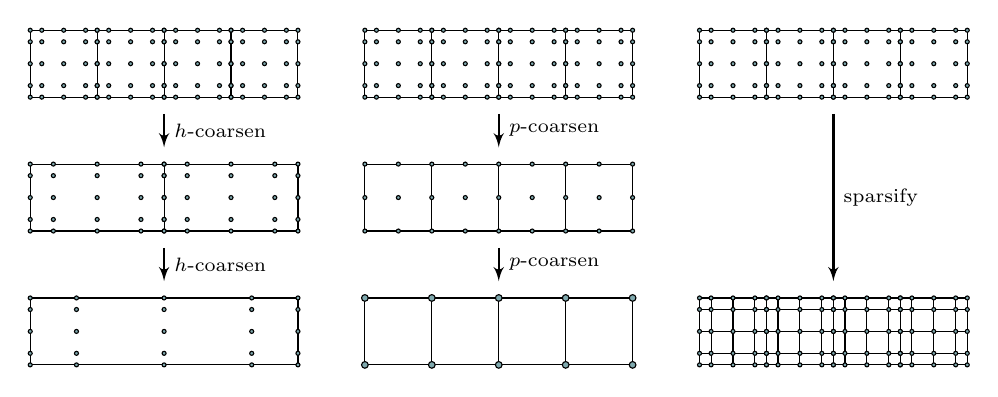
\begin{tikzpicture}[scale=0.85]
		% homg
		\draw (-5,4) grid +(4,1);
		\foreach \e in {-5,...,-2}
		\foreach \x in {0,0.1727,0.5,0.8273, 1.0} {
			\draw[fill=utsecblue] (\e+\x, 4) circle (0.03);
			\draw[fill=utsecblue] (\e+\x, 4.1727) circle (0.03);
			\draw[fill=utsecblue] (\e+\x, 4.5) circle (0.03);
			\draw[fill=utsecblue] (\e+\x, 4.8273) circle (0.03);
			\draw[fill=utsecblue] (\e+\x, 5) circle (0.03);
		}
		%\node at (5,4.5) {\small $p=4$};
		\draw[-latex',thick] (-3, 3.75) -- node[right] {{\scriptsize $h$-coarsen}} (-3, 3.25);
		\draw (-5,2) rectangle +(4,1);
		\draw (-3,2) -- (-3,3);
		\foreach \e in {-5,-3}
		\foreach \x in {0,0.1727,0.5,0.8273, 1.0} {
			\draw[fill=utsecblue] (\e+2*\x, 2) circle (0.03);
			\draw[fill=utsecblue] (\e+2*\x, 2.1727) circle (0.03);
			\draw[fill=utsecblue] (\e+2*\x, 2.5) circle (0.03);
			\draw[fill=utsecblue] (\e+2*\x, 2.8273) circle (0.03);
			\draw[fill=utsecblue] (\e+2*\x, 3) circle (0.03);
		}
		%\node at (5,2.5) {\small $p=2$};
	
		\draw[-latex',thick] (-3, 1.75) -- node[right] {{\scriptsize $h$-coarsen}} (-3, 1.25);
	
		\draw (-5,0) rectangle +(4,1);
		\foreach \x in {0,0.1727,0.5,0.8273, 1.0} {
			\draw[fill=utsecblue] (-5+4*\x, 0) circle (0.03);
			\draw[fill=utsecblue] (-5+4*\x, 0.1727) circle (0.03);
			\draw[fill=utsecblue] (-5+4*\x, 0.5) circle (0.03);
			\draw[fill=utsecblue] (-5+4*\x, 0.8273) circle (0.03);
			\draw[fill=utsecblue] (-5+4*\x, 1) circle (0.03);
		}
		
	%% p-multigrid
		\draw (0,4) grid +(4,1);
		\foreach \e in {0,...,3}
		\foreach \x in {0,0.1727,0.5,0.8273, 1.0} {
			\draw[fill=utsecblue] (\e+\x, 4) circle (0.03);
			\draw[fill=utsecblue] (\e+\x, 4.1727) circle (0.03);
			\draw[fill=utsecblue] (\e+\x, 4.5) circle (0.03);
			\draw[fill=utsecblue] (\e+\x, 4.8273) circle (0.03);
			\draw[fill=utsecblue] (\e+\x, 5) circle (0.03);
		}
		%\node at (5,4.5) {\small $p=4$};
	
		\draw[-latex',thick] (2, 3.75) -- node[right] {{\scriptsize $p$-coarsen}} (2, 3.25);
	
		\draw (0,2) grid +(4,1);
		\foreach \x in {0,0.5,...,4} {
			\draw[fill=utsecblue] (\x, 2) circle (0.03);
			\draw[fill=utsecblue] (\x, 2.5) circle (0.03);
			\draw[fill=utsecblue] (\x, 3) circle (0.03);
		}
		%\node at (5,2.5) {\small $p=2$};
	
		\draw[-latex',thick] (2, 1.75) -- node[right] {{\scriptsize $p$-coarsen}} (2, 1.25);
	
		\draw (0,0) grid +(4,1);
		\foreach \x in {0,1,2,3,4} {
			\draw[fill=utsecblue] (\x, 0) circle (0.05);
			\draw[fill=utsecblue] (\x, 1) circle (0.05);
		}
		%\node at (5,0.5) {\small $p=1$};
		
		%% collocated
			\draw (5,4) grid +(4,1);
			\foreach \e in {5,...,8}
			\foreach \x in {0,0.1727,0.5,0.8273, 1.0} {
				\draw[fill=utsecblue] (\e+\x, 4) circle (0.03);
				\draw[fill=utsecblue] (\e+\x, 4.1727) circle (0.03);
				\draw[fill=utsecblue] (\e+\x, 4.5) circle (0.03);
				\draw[fill=utsecblue] (\e+\x, 4.8273) circle (0.03);
				\draw[fill=utsecblue] (\e+\x, 5) circle (0.03);
			}
			%\node at (2, 1.8) {\tiny $p=4$};
	
			\draw[-latex',thick] (7, 3.75) -- node[right] {{\scriptsize sparsify}} (7, 1.25);
	
			\draw[step=0.5] (4.99,0) grid +(4.01,1);
			\draw (5,0.1727) -- (9,0.1727);
			\draw (5,0.8273) -- (9,0.8273);
			\foreach \e in {5,...,8} {
				\draw (\e+0.1727,0) -- (\e+0.1727,1);
				\draw (\e+0.8273,0) -- (\e+0.8273,1);
				\foreach \x in {0,0.1727,0.5,0.8273, 1.0} {
					\draw[fill=utsecblue] (\e+\x, 0) circle (0.03);
					\draw[fill=utsecblue] (\e+\x, 0.1727) circle (0.03);
					\draw[fill=utsecblue] (\e+\x, 0.5) circle (0.03);
					\draw[fill=utsecblue] (\e+\x, 0.8273) circle (0.03);
					\draw[fill=utsecblue] (\e+\x, 1) circle (0.03);
				}
			}
			% \node at (2, -0.2) {\tiny $p=1$ collocated with $p=4$};
		\end{tikzpicture}
		\caption{\label{fig:approaches} Different approaches
                  for high-order multigrid: high-order $h$-multigrid
                  (left), $p$-multigrid (middle) and low-order
                  preconditioned multigrid.}
\end{figure}

\subsection{$h$-multigrid}\label{subsec:h}
A direct approach to high-order multigrid is to use high-order
restriction and prolongation operators, and use the high-order
discretization of the operator for the residual computation on each
multigrid level.  A potential difficulty in this approach is that it
requires smoothers for matrices arising from high-order
discretization, which usually have less favorable properties compared
to their low order counterparts; For instance, high-order
discretizations of scalar elliptic operators are usually not
M-matrices, which is a useful property to prove the convergence of
smoothers such as Jacobi of Gauss-Seidel.  Due to the decreased
sparsity of high-order discretized systems, the efficient computation
of the residual can be a challenge. As a remedy, one can use
matrix-free methods which do not require to assemble system matrices
but rely on element-local computations. The performance of these
element-local computations can often be speed up using tensorized
finite element basis functions as common in spectral element methods;
see e.g.~\cite{DevilleFischerMund02}.


\subsection{$p$-multigrid}\label{subsec:p}
In the $p$-multigrid approach to high-order multigrid, one (initially)
does not coarsen the mesh geometrically, but coarsens the system by
reducing the polynomial order. Starting from an order-$p$ polynomial
basis (for simplicity, we assume here that $p$ is a power of 2), the
coarser grids correspond to polynomials of order $p/2, p/4,\ldots,1$,
followed by geometric coarsening of the $p=1$ grid (i.e., the usual
low order geometric multigrid). Decreasing the polynomial order is an
element-local operation and is particularly simple for discretizations
with nonconforming meshes. \gsnote{Is that actually true?}. As for
high-order $h$-multigrid, devising smoothers is a challenge for
$p$-multigrid.  Moreover, one often finds dependence of the
convergence factor on the order of the polynomial basis. \gsnote{We
  need a citation here.}

\subsection{Defect correction using lower-order operator}\label{subsec:low}
In a defect correction approach (see
\cite{TrottenbergOosterleeSchuller01}), the high-order defect is
iteratively corrected using a low order operator obtained by
overlaying the high-order nodes with a low order (typically linear)
finite element mesh.  This construction of a low-order preconditioner
based on the nodes of the high-order discretization is used. for
instance
in~\cite{Brown10,Kim07,DevilleMund90,HeysManteuffelMcCormickEtAl05}.
The resulting method is nearly independent of $p$, but this low-order
preconditioning is not work optimal and the convergence factors can be
lower than when multigrid is applied directly to the high-order
operator. \gsnote{Reference or remove statement.} Defect correction
only requires computation of the residual for the high-order
discretized operator, while smoothing is based on the low order
discretized operator, which is sparse and thus faster to apply.

Due to the non evenly spaced node spacing inherited from the
high-order discretization, the solution of the low order system is not
straightforward. One possible approach to solve the low order system
is to rely on algebraic multigrid,
e.g.,~\cite{Brown10,HeysManteuffelMcCormickEtAl05}; this approach is
particularly attractive for high-order discretizations on unstructured
meshes, where the construction of a grid hierarchy from geometric
coarsening can be very difficult. For structured grids such as the
ones used for the test problems in Section~\ref{sec:numerics}, a
geometric multigrid method can be devised that either copes with the
non evenly spaced points (which can be challenging) or replaces them
by evenly spaced points---we experiment with the latter option in
Section~\ref{sec:numerics}.

Note that, for nonconforming meshes, constructing the low order
operator can be a technical task at edges and faces of different size;
while the basis functions for the high-order operators can be made
continuous through the use of algebraic constraints at nonconforming
faces, the corresponding low order discretization has discontinuities
at nonconforming faces.



% multigrid cycles are faster compared to high
%order $h$-multigrid or $p$-multigrid discussed in
%Section~\ref{subsec:h} and Section~\ref{subsec:p}, respectively.

%Standard multigrid is then used for the low order operator, which has
%more favorable sparsity properties and thus allows for standard
%smoothers.
%  Thus, the speedup for a full multigrid cycle when using the
%low order operator is limited.


%The advantages of doing
%this are mainly in the simplicity of the approach and the availability
%of parallel multigrid solvers capable of solving such lower-order
%operators.
% The sparsity of the lower-order operators also permits the
%use of AMG for solving the lower-order operators, possibly obtained
%via discretizations on unstructured meshes.


% **********************************************************
\section{Smoothers}
Here, we summarize the smoothers used in our numerical experiments, for
which we restrict ourselves to the point smoothers summarized in
Section~\ref{subsec:ptsmoothers}. For completeness of the
presentation, we comment on Schwarz-type smoothers in
Section~\ref{subsec:schwarz}.


\subsection{Point smoothers}\label{subsec:ptsmoothers}
In our numerical tests, we compare the Jacobi and the
symmetric successive over relaxation (SSOR) smoothers
(see~\cite{TrottenbergOosterleeSchuller01}), as well as a
Chebyshev-accelerated Jacobi smoother~\cite{....}. All of these
smoothers require the diagonal of the system matrix; if matrices are
not assembled (i.e., in a matrix-free approach), these diagonal
entries must be precomputed in a setup step.  Note that the
parallelization of Gauss-Seidel smoothers (such as SSOR) requires
coloring of unknowns at parallel boundaries, and, compared to Jacobi
smoothing, more complex communication in a distributed memory
implementation. In parallel, the Chebyshev-accelerated Jacobi method
is an attractive alternative to SSOR; it can significantly improve
over Jacobi smoothing, while being as simple to
implement~\cite{AdamsBrezinaHuEtAl03}. However, the acceleration of
Jacobi smoothing with Chebyshev polynomials requires estimation of the
maximum eigenvalues of the system matrix, which has to be done in a
setup step using, for instance, a power method.
\begin{figure}
	\centering
	\begin{subfigure}[b]{0.49\textwidth}
		% This file was created by matlab2tikz v0.3.3.
% Copyright (c) 2008--2013, Nico Schlmer <nico.schloemer@gmail.com>
% All rights reserved.
% 
% The latest updates can be retrieved from
%   http://www.mathworks.com/matlabcentral/fileexchange/22022-matlab2tikz
% where you can also make suggestions and rate matlab2tikz.
% 
% 
% 

% defining custom colors
\definecolor{mycolor1}{rgb}{1,0,1}

\begin{tikzpicture}[scale=0.2]

\begin{axis}[%
width=10.8672222222222in,
height=10.2056111111111in,
scale only axis,
xmin=0,
xmax=1100,
xmajorgrids,
xmajorticks=false,
ymode=log,
ymin=1e-08,
ymax=4,
% yminorticks=false,
ymajorgrids,
% yminorgrids,
% title={$\text{N = 33}^\text{2}\text{ , p = 1}$}
]
\addplot [
color=black,
solid,thick,
forget plot
]
table[row sep=crcr]{
1 1.00000000000001\\
2 0.999999999999995\\
3 0.999999999999993\\
4 1\\
5 1.00000000000001\\
6 1\\
7 1\\
8 1\\
9 1\\
10 1\\
11 0.999999999999993\\
12 0.999999999999996\\
13 0.999999999999989\\
14 0.999999999999997\\
15 0.999999999999997\\
16 1\\
17 1.00000000000001\\
18 1\\
19 1\\
20 1\\
21 1\\
22 0.999999999999994\\
23 1\\
24 1\\
25 0.999999999999998\\
26 1.00000000000001\\
27 1\\
28 1\\
29 1.00000000000001\\
30 1\\
31 0.999999999999997\\
32 1.00000000000001\\
33 0.999999999999999\\
34 1\\
35 1\\
36 0.999999999999998\\
37 0.999999999999999\\
38 1.00000000000001\\
39 1.00000000000001\\
40 0.999999999999998\\
41 1\\
42 0.999999999999996\\
43 0.999999999999987\\
44 1\\
45 1\\
46 1.00000000000001\\
47 0.999999999999997\\
48 1\\
49 1\\
50 0.999999999999999\\
51 0.999999999999993\\
52 0.999999999999997\\
53 1\\
54 1\\
55 0.999999999999994\\
56 0.999999999999999\\
57 1\\
58 1\\
59 1\\
60 0.999999999999999\\
61 1.00000000000001\\
62 1\\
63 0.999999999999999\\
64 0.999999999999997\\
65 1\\
66 0.99999999999999\\
67 1\\
68 0.999999999999994\\
69 1\\
70 0.999999999999993\\
71 0.999999999999995\\
72 1.00000000000001\\
73 0.999999999999997\\
74 1\\
75 1\\
76 1.00000000000001\\
77 1\\
78 1\\
79 1\\
80 0.999999999999996\\
81 1\\
82 1\\
83 1\\
84 1\\
85 0.999999999999998\\
86 0.999999999999996\\
87 1\\
88 0.999999999999999\\
89 0.999999999999997\\
90 1.00000000000001\\
91 1\\
92 0.999999999999995\\
93 1.00000000000001\\
94 1\\
95 0.999999999999991\\
96 1\\
97 1\\
98 1\\
99 0.999999999999991\\
100 1\\
101 1.00000000000001\\
102 1\\
103 0.99999999999999\\
104 0.999999999999999\\
105 1\\
106 0.999999999999999\\
107 1.00000000000001\\
108 1\\
109 0.99999999999999\\
110 0.99999999999999\\
111 1.00000000000001\\
112 0.999999999999999\\
113 1.00000000000001\\
114 0.999999999999994\\
115 0.999999999999996\\
116 0.999999999999992\\
117 1\\
118 1.00000000000001\\
119 0.999999999999998\\
120 0.999999999999995\\
121 1\\
122 1\\
123 1\\
124 0.999999999999998\\
125 1.00000000000001\\
126 0.999999999999999\\
127 0.999999999999992\\
128 0.999999999999999\\
129 1\\
130 0.999999999999999\\
131 1.00000000000001\\
132 0.999999999999985\\
133 0.999999999999994\\
134 1.00000000000001\\
135 0.999999999999996\\
136 1.00000000000001\\
137 1\\
138 0.999999999999994\\
139 1\\
140 0.999999999999984\\
141 1\\
142 0.999999999999998\\
143 0.999999999999999\\
144 1.00000000000001\\
145 1.00000000000001\\
146 1\\
147 0.999999999999995\\
148 0.999999999999995\\
149 1.00000000000001\\
150 0.999999999999996\\
151 1\\
152 0.999999999999999\\
153 1.00000000000001\\
154 1\\
155 0.999999999999991\\
156 0.999999999999996\\
157 1\\
158 1.00000000000001\\
159 0.999999999999995\\
160 1\\
161 0.999999999999992\\
162 0.999999999999993\\
163 1\\
164 0.999999999999999\\
165 0.999999999999995\\
166 0.999999999999998\\
167 0.999999999999994\\
168 0.999999999999997\\
169 0.999999999999999\\
170 0.999999999999992\\
171 0.999999999999996\\
172 1\\
173 1.00000000000001\\
174 1.00000000000001\\
175 1\\
176 1\\
177 1.00000000000001\\
178 0.999999999999997\\
179 1\\
180 1.00000000000002\\
181 1.00000000000001\\
182 1\\
183 1.00000000000001\\
184 0.999999999999995\\
185 0.999999999999993\\
186 0.999999999999998\\
187 0.999999999999993\\
188 1\\
189 1\\
190 1.00000000000001\\
191 0.999999999999994\\
192 1\\
193 1\\
194 1\\
195 0.999999999999998\\
196 1\\
197 0.999999999999999\\
198 1\\
199 1\\
200 1\\
201 0.999999999999995\\
202 1\\
203 1.00000000000001\\
204 1\\
205 1\\
206 0.999999999999991\\
207 1\\
208 0.999999999999996\\
209 0.999999999999998\\
210 0.999999999999998\\
211 0.999999999999998\\
212 1.00000000000001\\
213 1\\
214 0.999999999999997\\
215 0.999999999999988\\
216 1\\
217 1\\
218 1.00000000000001\\
219 1.00000000000001\\
220 0.999999999999991\\
221 0.999999999999996\\
222 0.99999999999999\\
223 0.999999999999997\\
224 0.999999999999997\\
225 0.999999999999999\\
226 0.999999999999998\\
227 0.999999999999986\\
228 1\\
229 0.999999999999997\\
230 0.999999999999997\\
231 0.999999999999983\\
232 0.999999999999995\\
233 1.00000000000001\\
234 0.999999999999997\\
235 0.999999999999996\\
236 0.999999999999999\\
237 0.999999999999988\\
238 1\\
239 0.999999999999998\\
240 0.99999999999999\\
241 1\\
242 0.999999999999986\\
243 0.999999999999996\\
244 1\\
245 0.999999999999993\\
246 1\\
247 1.00000000000001\\
248 1\\
249 0.999999999999994\\
250 1\\
251 1\\
252 0.999999999999995\\
253 0.999999999999995\\
254 1.00000000000001\\
255 0.999999999999997\\
256 0.999999999999997\\
257 1\\
258 1\\
259 0.999999999999996\\
260 0.999999999999995\\
261 1.00000000000001\\
262 1.00000000000001\\
263 0.999999999999994\\
264 1.00000000000001\\
265 1\\
266 1.00000000000001\\
267 0.999999999999995\\
268 0.999999999999999\\
269 1\\
270 1.00000000000001\\
271 1\\
272 0.999999999999998\\
273 0.999999999999999\\
274 1\\
275 1.00000000000001\\
276 0.999999999999999\\
277 0.999999999999998\\
278 1.00000000000001\\
279 1.00000000000001\\
280 0.999999999999996\\
281 0.99999999999999\\
282 1\\
283 1\\
284 0.999999999999998\\
285 1.00000000000001\\
286 0.999999999999993\\
287 1.00000000000001\\
288 1\\
289 0.999999999999992\\
290 0.999999999999995\\
291 1.00000000000001\\
292 0.999999999999999\\
293 0.999999999999996\\
294 0.999999999999989\\
295 1.00000000000001\\
296 0.999999999999988\\
297 0.999999999999996\\
298 0.999999999999997\\
299 0.999999999999998\\
300 1\\
301 1.00000000000001\\
302 1\\
303 0.999999999999999\\
304 1\\
305 0.999999999999992\\
306 0.999999999999996\\
307 1\\
308 0.999999999999996\\
309 1\\
310 1\\
311 0.99999999999999\\
312 1\\
313 1\\
314 1\\
315 1.00000000000001\\
316 0.999999999999993\\
317 0.999999999999991\\
318 1.00000000000001\\
319 0.999999999999983\\
320 1.00000000000002\\
321 0.999999999999994\\
322 0.999999999999992\\
323 0.99999999999999\\
324 1.00000000000001\\
325 1\\
326 1\\
327 1.00000000000001\\
328 0.999999999999997\\
329 0.999999999999982\\
330 1\\
331 0.999999999999995\\
332 0.999999999999993\\
333 0.999999999999997\\
334 0.999999999999999\\
335 0.999999999999997\\
336 1.00000000000001\\
337 0.999999999999986\\
338 1\\
339 1.00000000000001\\
340 0.999999999999987\\
341 0.999999999999993\\
342 0.999999999999997\\
343 0.999999999999999\\
344 1.00000000000001\\
345 1\\
346 0.999999999999999\\
347 0.999999999999997\\
348 1\\
349 1.00000000000001\\
350 0.999999999999995\\
351 1\\
352 0.999999999999994\\
353 0.999999999999989\\
354 0.999999999999996\\
355 0.999999999999996\\
356 1.00000000000001\\
357 0.999999999999999\\
358 0.999999999999999\\
359 1.00000000000001\\
360 1\\
361 0.999999999999997\\
362 0.999999999999992\\
363 0.999999999999994\\
364 1.00000000000001\\
365 1.00000000000001\\
366 1.00000000000001\\
367 0.999999999999996\\
368 1\\
369 1.00000000000001\\
370 1\\
371 0.999999999999992\\
372 1\\
373 1\\
374 1.00000000000001\\
375 1\\
376 0.999999999999993\\
377 0.999999999999996\\
378 1\\
379 0.999999999999991\\
380 0.999999999999995\\
381 0.999999999999992\\
382 1\\
383 1\\
384 0.999999999999985\\
385 0.999999999999999\\
386 1.00000000000001\\
387 1.00000000000001\\
388 1.00000000000001\\
389 0.999999999999992\\
390 1\\
391 1\\
392 0.999999999999997\\
393 0.999999999999988\\
394 0.999999999999984\\
395 1.00000000000001\\
396 1\\
397 1.00000000000001\\
398 0.999999999999997\\
399 0.999999999999994\\
400 1\\
401 1\\
402 0.999999999999993\\
403 1\\
404 0.999999999999997\\
405 1\\
406 1.00000000000001\\
407 0.999999999999994\\
408 1.00000000000001\\
409 0.999999999999992\\
410 1\\
411 0.999999999999999\\
412 1\\
413 0.999999999999989\\
414 0.999999999999996\\
415 0.999999999999997\\
416 1.00000000000001\\
417 0.999999999999996\\
418 1.00000000000001\\
419 1\\
420 1\\
421 1\\
422 0.999999999999985\\
423 1.00000000000001\\
424 0.999999999999996\\
425 0.999999999999995\\
426 0.99999999999999\\
427 0.999999999999999\\
428 0.999999999999989\\
429 1\\
430 0.999999999999996\\
431 0.999999999999988\\
432 0.999999999999991\\
433 0.999999999999986\\
434 1\\
435 1.00000000000001\\
436 0.999999999999998\\
437 0.999999999999997\\
438 1\\
439 0.999999999999996\\
440 0.999999999999994\\
441 0.999999999999997\\
442 0.999999999999989\\
443 0.999999999999988\\
444 1\\
445 1\\
446 0.99999999999999\\
447 1\\
448 1\\
449 1\\
450 0.999999999999998\\
451 0.999999999999991\\
452 0.999999999999991\\
453 1.00000000000001\\
454 0.999999999999989\\
455 0.999999999999988\\
456 1.00000000000001\\
457 1.00000000000001\\
458 1\\
459 0.999999999999994\\
460 1.00000000000001\\
461 1\\
462 1\\
463 1\\
464 0.999999999999998\\
465 1\\
466 0.999999999999978\\
467 1\\
468 0.999999999999998\\
469 1\\
470 1\\
471 0.999999999999998\\
472 0.999999999999993\\
473 1\\
474 0.999999999999999\\
475 1.00000000000001\\
476 0.999999999999981\\
477 0.999999999999999\\
478 0.999999999999999\\
479 1\\
480 0.999999999999992\\
481 1\\
482 1\\
483 0.999999999999993\\
484 1\\
485 1.00000000000001\\
486 0.999999999999999\\
487 0.999999999999994\\
488 0.999999999999996\\
489 1\\
490 0.999999999999996\\
491 1\\
492 1\\
493 0.999999999999992\\
494 0.999999999999993\\
495 1.00000000000001\\
496 0.999999999999996\\
497 0.999999999999994\\
498 1\\
499 0.999999999999989\\
500 1\\
501 1\\
502 0.99999999999999\\
503 1\\
504 1\\
505 1.00000000000001\\
506 1\\
507 1.00000000000001\\
508 0.999999999999995\\
509 1.00000000000001\\
510 0.999999999999996\\
511 1\\
512 0.999999999999994\\
513 0.999999999999992\\
514 1\\
515 1\\
516 1\\
517 0.999999999999995\\
518 0.999999999999983\\
519 0.99999999999999\\
520 0.999999999999993\\
521 1.00000000000001\\
522 0.999999999999999\\
523 1.00000000000001\\
524 1.00000000000001\\
525 0.999999999999999\\
526 1\\
527 1\\
528 0.999999999999999\\
529 1\\
530 0.999999999999996\\
531 0.999999999999996\\
532 0.999999999999994\\
533 1.00000000000001\\
534 0.999999999999995\\
535 1\\
536 1\\
537 1.00000000000001\\
538 0.999999999999987\\
539 0.999999999999995\\
540 0.999999999999994\\
541 1\\
542 0.999999999999991\\
543 0.999999999999995\\
544 0.999999999999995\\
545 0.999999999999988\\
546 1\\
547 0.999999999999989\\
548 0.99999999999999\\
549 0.999999999999995\\
550 0.999999999999993\\
551 0.999999999999993\\
552 0.99999999999999\\
553 1\\
554 1\\
555 0.999999999999986\\
556 1\\
557 1.00000000000001\\
558 0.999999999999994\\
559 1.00000000000001\\
560 0.999999999999986\\
561 1\\
562 1.00000000000001\\
563 1\\
564 0.999999999999994\\
565 0.999999999999998\\
566 0.999999999999987\\
567 1\\
568 0.999999999999999\\
569 1.00000000000001\\
570 0.999999999999986\\
571 1\\
572 0.999999999999995\\
573 1\\
574 1.00000000000001\\
575 1.00000000000001\\
576 0.999999999999987\\
577 0.999999999999999\\
578 0.999999999999996\\
579 1\\
580 0.999999999999996\\
581 1\\
582 1\\
583 0.999999999999983\\
584 0.999999999999992\\
585 1.00000000000001\\
586 1\\
587 0.999999999999999\\
588 1.00000000000001\\
589 1.00000000000001\\
590 0.999999999999997\\
591 0.999999999999996\\
592 1\\
593 0.999999999999998\\
594 0.999999999999991\\
595 0.999999999999996\\
596 1\\
597 1.00000000000001\\
598 1.00000000000001\\
599 0.999999999999998\\
600 0.999999999999995\\
601 1.00000000000001\\
602 0.999999999999998\\
603 0.999999999999998\\
604 0.999999999999999\\
605 0.999999999999997\\
606 1.00000000000001\\
607 0.999999999999992\\
608 1.00000000000001\\
609 1\\
610 0.99999999999999\\
611 1.00000000000001\\
612 1\\
613 0.999999999999999\\
614 0.999999999999994\\
615 1.00000000000001\\
616 0.999999999999999\\
617 0.999999999999998\\
618 1\\
619 0.999999999999995\\
620 1.00000000000001\\
621 0.999999999999996\\
622 1\\
623 1.00000000000001\\
624 1\\
625 1\\
626 1.00000000000001\\
627 0.99999999999999\\
628 0.999999999999986\\
629 0.999999999999991\\
630 0.999999999999997\\
631 1.00000000000001\\
632 1\\
633 1.00000000000002\\
634 0.999999999999998\\
635 0.999999999999996\\
636 1\\
637 0.999999999999984\\
638 1.00000000000001\\
639 0.999999999999998\\
640 1\\
641 1.00000000000003\\
642 1.00000000000001\\
643 1\\
644 0.999999999999995\\
645 0.999999999999976\\
646 1\\
647 0.999999999999994\\
648 1.00000000000001\\
649 1.00000000000001\\
650 0.999999999999992\\
651 1\\
652 1\\
653 0.999999999999997\\
654 0.999999999999992\\
655 0.999999999999998\\
656 1.00000000000001\\
657 0.999999999999992\\
658 0.999999999999984\\
659 1.00000000000002\\
660 1\\
661 1\\
662 0.99999999999999\\
663 1\\
664 0.999999999999996\\
665 1\\
666 1.00000000000001\\
667 0.999999999999997\\
668 1.00000000000001\\
669 1\\
670 1\\
671 0.999999999999994\\
672 0.999999999999989\\
673 0.999999999999995\\
674 0.999999999999993\\
675 0.999999999999998\\
676 0.999999999999998\\
677 1.00000000000001\\
678 0.999999999999994\\
679 1.00000000000001\\
680 1\\
681 0.999999999999983\\
682 1\\
683 1.00000000000001\\
684 0.999999999999988\\
685 1\\
686 1\\
687 0.999999999999988\\
688 0.999999999999991\\
689 0.999999999999995\\
690 1.00000000000001\\
691 1.00000000000001\\
692 1.00000000000001\\
693 1.00000000000001\\
694 0.999999999999999\\
695 1\\
696 1\\
697 1\\
698 1.00000000000001\\
699 1.00000000000001\\
700 0.999999999999998\\
701 1\\
702 0.999999999999987\\
703 1\\
704 0.999999999999982\\
705 1\\
706 1\\
707 0.999999999999986\\
708 1.00000000000001\\
709 0.999999999999995\\
710 0.999999999999998\\
711 1\\
712 0.999999999999991\\
713 1\\
714 0.999999999999991\\
715 0.999999999999993\\
716 1.00000000000001\\
717 1\\
718 0.999999999999987\\
719 0.999999999999992\\
720 1.00000000000001\\
721 0.999999999999993\\
722 1.00000000000001\\
723 1\\
724 0.999999999999996\\
725 1\\
726 1\\
727 1.00000000000001\\
728 1.00000000000001\\
729 1.00000000000001\\
730 0.999999999999996\\
731 1.00000000000002\\
732 0.999999999999992\\
733 1\\
734 0.999999999999986\\
735 0.999999999999991\\
736 1.00000000000001\\
737 1.00000000000001\\
738 1.00000000000001\\
739 0.999999999999993\\
740 1\\
741 1.00000000000002\\
742 0.999999999999989\\
743 0.999999999999998\\
744 1\\
745 1\\
746 1.00000000000002\\
747 0.999999999999997\\
748 1\\
749 1\\
750 0.999999999999999\\
751 0.999999999999994\\
752 1\\
753 0.999999999999995\\
754 0.999999999999996\\
755 1.00000000000001\\
756 0.999999999999992\\
757 1.00000000000001\\
758 1.00000000000001\\
759 1.00000000000001\\
760 0.999999999999999\\
761 1.00000000000002\\
762 0.999999999999996\\
763 1\\
764 0.99999999999999\\
765 1.00000000000001\\
766 0.999999999999978\\
767 0.999999999999993\\
768 0.999999999999997\\
769 0.999999999999993\\
770 1\\
771 0.999999999999993\\
772 0.99999999999999\\
773 1.00000000000002\\
774 1.00000000000002\\
775 1\\
776 0.999999999999989\\
777 1.00000000000001\\
778 1\\
779 0.999999999999981\\
780 1\\
781 0.999999999999985\\
782 1.00000000000001\\
783 1\\
784 0.999999999999986\\
785 0.999999999999988\\
786 0.999999999999988\\
787 1.00000000000001\\
788 1.00000000000002\\
789 1\\
790 1\\
791 1.00000000000001\\
792 0.999999999999995\\
793 1.00000000000002\\
794 1.00000000000001\\
795 0.999999999999996\\
796 0.999999999999979\\
797 0.999999999999994\\
798 0.999999999999999\\
799 1.00000000000001\\
800 0.999999999999997\\
801 0.99999999999998\\
802 1.00000000000001\\
803 0.999999999999997\\
804 0.999999999999985\\
805 0.99999999999999\\
806 1\\
807 1.00000000000001\\
808 1.00000000000001\\
809 1\\
810 0.99999999999998\\
811 0.999999999999987\\
812 1.00000000000001\\
813 0.999999999999995\\
814 1.00000000000001\\
815 0.999999999999995\\
816 0.99999999999998\\
817 0.999999999999997\\
818 1.00000000000001\\
819 0.999999999999996\\
820 0.99999999999999\\
821 0.999999999999992\\
822 0.999999999999989\\
823 0.999999999999997\\
824 0.999999999999994\\
825 0.999999999999979\\
826 1.00000000000001\\
827 0.999999999999999\\
828 1.00000000000001\\
829 1.00000000000001\\
830 0.999999999999999\\
831 0.999999999999998\\
832 0.999999999999998\\
833 1.00000000000001\\
834 1\\
835 1.00000000000001\\
836 1\\
837 0.999999999999996\\
838 0.999999999999997\\
839 0.999999999999995\\
840 1.00000000000001\\
841 0.999999999999995\\
842 1\\
843 1.00000000000001\\
844 0.999999999999992\\
845 1\\
846 1\\
847 0.999999999999981\\
848 0.999999999999989\\
849 1.00000000000002\\
850 1.00000000000001\\
851 1\\
852 0.999999999999995\\
853 1\\
854 0.999999999999991\\
855 0.999999999999991\\
856 0.999999999999992\\
857 1.00000000000001\\
858 1.00000000000002\\
859 0.999999999999994\\
860 1.00000000000001\\
861 0.999999999999992\\
862 0.999999999999996\\
863 1\\
864 0.999999999999998\\
865 0.999999999999999\\
866 0.999999999999999\\
867 0.999999999999993\\
868 1\\
869 1\\
870 1.00000000000001\\
871 0.999999999999995\\
872 0.999999999999986\\
873 1\\
874 1.00000000000001\\
875 0.999999999999992\\
876 1.00000000000001\\
877 0.999999999999997\\
878 1\\
879 1.00000000000001\\
880 1\\
881 1.00000000000001\\
882 1\\
883 1.00000000000001\\
884 0.999999999999992\\
885 0.999999999999998\\
886 1.00000000000002\\
887 1.00000000000001\\
888 0.999999999999992\\
889 0.99999999999999\\
890 0.999999999999995\\
891 1.00000000000002\\
892 0.999999999999993\\
893 0.999999999999998\\
894 1.00000000000001\\
895 0.99999999999999\\
896 0.999999999999995\\
897 1.00000000000002\\
898 0.999999999999999\\
899 0.999999999999996\\
900 1.00000000000001\\
901 1\\
902 0.999999999999999\\
903 0.999999999999996\\
904 1.00000000000001\\
905 1.00000000000001\\
906 0.999999999999998\\
907 1.00000000000001\\
908 0.999999999999996\\
909 1\\
910 0.999999999999998\\
911 0.999999999999992\\
912 1\\
913 0.99999999999999\\
914 0.999999999999981\\
915 1\\
916 1.00000000000001\\
917 1\\
918 1\\
919 1.00000000000001\\
920 0.999999999999998\\
921 0.999999999999996\\
922 0.999999999999996\\
923 0.99999999999999\\
924 0.999999999999998\\
925 1\\
926 1.00000000000002\\
927 1.00000000000001\\
928 0.999999999999985\\
929 1.00000000000001\\
930 0.999999999999981\\
931 0.999999999999975\\
932 1.00000000000001\\
933 0.999999999999993\\
934 0.99999999999999\\
935 0.999999999999993\\
936 0.999999999999982\\
937 0.999999999999997\\
938 1\\
939 0.99999999999999\\
940 0.999999999999973\\
941 1.00000000000001\\
942 0.999999999999994\\
943 0.999999999999988\\
944 0.999999999999993\\
945 1.00000000000001\\
946 1.00000000000001\\
947 1\\
948 1.00000000000001\\
949 0.999999999999998\\
950 1\\
951 0.999999999999993\\
952 1.00000000000001\\
953 1.00000000000001\\
954 0.999999999999987\\
955 0.999999999999999\\
956 1.00000000000001\\
957 1.00000000000001\\
958 1.00000000000001\\
959 0.999999999999988\\
960 1\\
961 0.999999999999991\\
962 0.999999999999991\\
963 1.00000000000001\\
964 1\\
965 0.999999999999992\\
966 0.999999999999994\\
967 1\\
968 1.00000000000002\\
969 0.999999999999991\\
970 1\\
971 0.99999999999999\\
972 0.999999999999989\\
973 0.999999999999988\\
974 0.999999999999978\\
975 0.999999999999996\\
976 0.999999999999993\\
977 0.999999999999999\\
978 1\\
979 0.99999999999999\\
980 1.00000000000001\\
981 0.999999999999992\\
982 1\\
983 1.00000000000001\\
984 0.999999999999991\\
985 1.00000000000001\\
986 1.00000000000001\\
987 1\\
988 0.999999999999985\\
989 1.00000000000001\\
990 1\\
991 0.999999999999992\\
992 0.999999999999998\\
993 1.00000000000001\\
994 0.999999999999993\\
995 0.999999999999988\\
996 0.999999999999996\\
997 0.999999999999982\\
998 0.999999999999994\\
999 1.00000000000001\\
1000 0.999999999999992\\
1001 0.999999999999989\\
1002 0.999999999999997\\
1003 1\\
1004 0.999999999999994\\
1005 1\\
1006 1\\
1007 0.999999999999998\\
1008 1\\
1009 1\\
1010 1\\
1011 1\\
1012 1.00000000000001\\
1013 1.00000000000001\\
1014 1\\
1015 1\\
1016 1.00000000000002\\
1017 1\\
1018 1.00000000000001\\
1019 1\\
1020 1\\
1021 0.999999999999999\\
1022 0.999999999999998\\
1023 1\\
1024 1\\
1025 1\\
1026 0.999999999999996\\
1027 0.999999999999998\\
1028 1.00000000000001\\
1029 1\\
1030 1\\
1031 0.999999999999997\\
1032 1\\
1033 1\\
1034 1\\
1035 1\\
1036 1.00000000000001\\
1037 0.999999999999987\\
1038 1.00000000000001\\
1039 0.999999999999994\\
1040 1.00000000000001\\
1041 1.00000000000002\\
1042 1\\
1043 1.00000000000001\\
1044 1.00000000000001\\
1045 0.999999999999985\\
1046 1\\
1047 0.999999999999997\\
1048 0.999999999999996\\
1049 0.999999999999998\\
1050 0.999999999999996\\
1051 0.999999999999999\\
1052 0.999999999999992\\
1053 1.00000000000001\\
1054 1.00000000000001\\
1055 0.999999999999999\\
1056 1.00000000000001\\
1057 0.999999999999993\\
1058 1\\
1059 0.999999999999995\\
1060 0.999999999999999\\
1061 0.999999999999989\\
1062 0.999999999999992\\
1063 1.00000000000002\\
1064 1.00000000000001\\
1065 0.999999999999988\\
1066 0.999999999999998\\
1067 1\\
1068 0.999999999999982\\
1069 1.00000000000002\\
1070 1\\
1071 1\\
1072 0.999999999999986\\
1073 0.999999999999993\\
1074 0.999999999999986\\
1075 0.999999999999999\\
1076 1.00000000000001\\
1077 1\\
1078 0.999999999999995\\
1079 1.00000000000001\\
1080 0.999999999999994\\
1081 0.999999999999988\\
1082 1\\
1083 1\\
1084 1.00000000000001\\
1085 1\\
1086 1\\
1087 1.00000000000001\\
1088 1\\
1089 1.00000000000001\\
};
\addplot [
color=blue!40,
opacity=0.5,
solid,thick,
forget plot
]
table[row sep=crcr]{
1 0.980713521202408\\
2 1.06967247781685\\
3 1.01074460777748\\
4 0.814558984908198\\
5 0.854085403861034\\
6 0.988327876449661\\
7 1.26210254083276\\
8 0.82648824045788\\
9 0.72638292820056\\
10 0.845216572596158\\
11 1.12810521673016\\
12 0.862430226969949\\
13 0.922621450678224\\
14 0.546142667861782\\
15 1.04624881081685\\
16 1.44264566335871\\
17 0.890813823018154\\
18 0.825195421810088\\
19 0.972689994034164\\
20 0.840073271031526\\
21 0.54746876881327\\
22 0.885164107054228\\
23 0.856453648178297\\
24 0.572511931539663\\
25 0.72269228083296\\
26 0.661882484688336\\
27 0.841436220135634\\
28 0.690739447606068\\
29 1.11217532509538\\
30 0.761360313297711\\
31 1.47574204665726\\
32 0.772019139623085\\
33 0.716914448153119\\
34 0.608636992575809\\
35 0.847301259593692\\
36 0.998936821561583\\
37 0.814408539911699\\
38 0.761148211991405\\
39 0.768266875304758\\
40 0.671287573790122\\
41 0.772365924224308\\
42 0.671366711406911\\
43 0.623126127796091\\
44 0.731976495581535\\
45 0.64666033818859\\
46 0.541452211793102\\
47 0.795622208231103\\
48 0.750571108146117\\
49 0.148284228951537\\
50 0.707688722222302\\
51 0.57972503033556\\
52 0.641378112511217\\
53 1.11630605614296\\
54 0.763769384695137\\
55 0.690178961855084\\
56 0.551564779839249\\
57 0.812454314904717\\
58 0.951063712718902\\
59 0.573885030980975\\
60 0.471442460511363\\
61 0.617230474227117\\
62 0.651976932780021\\
63 0.470094455781772\\
64 0.591401428089076\\
65 0.59469155859514\\
66 0.730241260941873\\
67 0.411478646733708\\
68 0.477354226221245\\
69 0.553581249384703\\
70 0.702853208878481\\
71 0.300948090703062\\
72 0.588376538892773\\
73 0.697257364486752\\
74 0.0922984566256063\\
75 0.671703210294353\\
76 0.562797073001564\\
77 0.771761534634918\\
78 0.639610492038428\\
79 0.427328431448559\\
80 0.673463399884632\\
81 0.399531185776909\\
82 0.637522030668187\\
83 0.521022957796184\\
84 0.568549903544838\\
85 0.64674595632234\\
86 0.528361387421026\\
87 0.469553594644218\\
88 0.416289000877996\\
89 0.675110042066188\\
90 0.363140202052729\\
91 0.519959651938607\\
92 0.318020780692982\\
93 0.41342887437702\\
94 0.439251197750145\\
95 0.455437622805426\\
96 0.0908623097895471\\
97 0.502396308113828\\
98 0.341599393752732\\
99 0.0769927252969812\\
100 0.510891587425536\\
101 0.365504952256892\\
102 0.602811423993932\\
103 0.1673665046359\\
104 0.360593351758639\\
105 0.219188011609347\\
106 0.6601374441488\\
107 0.372779581898078\\
108 0.512151474760079\\
109 0.508446481447564\\
110 0.0519998558438209\\
111 0.204616599771736\\
112 0.504490813022762\\
113 0.482942475102297\\
114 0.281854006330257\\
115 0.291358398169106\\
116 0.279901253518019\\
117 0.440519192006014\\
118 0.350385431193792\\
119 0.343643099701131\\
120 0.391038149657218\\
121 0.188254131176562\\
122 0.00196695318600193\\
123 0.39203023639749\\
124 0.371281246412939\\
125 0.348706880722673\\
126 0.470856707723136\\
127 0.198408930322762\\
128 0.4595870551067\\
129 0.397509358798262\\
130 0.329555606779175\\
131 0.35788874971746\\
132 0.3538401487761\\
133 0.311178249809784\\
134 0.321937706624937\\
135 0.172731420137884\\
136 0.332394318247545\\
137 0.352890439368259\\
138 0.46277344147902\\
139 0.262984400709633\\
140 0.43507075913976\\
141 0.0111373080159735\\
142 0.246816726768119\\
143 0.0736765126957322\\
144 0.323394492720427\\
145 0.237011155747702\\
146 0.434050187514141\\
147 0.329701374501989\\
148 0.328046809999189\\
149 0.317659312532322\\
150 0.455449842660393\\
151 0.236303001125153\\
152 0.232806893459371\\
153 0.00399783704814171\\
154 0.217765684454585\\
155 0.405419046979958\\
156 0.0251635095459299\\
157 0.277470937210116\\
158 0.145337038775503\\
159 0.105538227690758\\
160 0.280619371098369\\
161 0.180477366708081\\
162 0.0687637204014991\\
163 0.0969310795963671\\
164 0.270109772910862\\
165 0.165600120538721\\
166 0.0895384763678585\\
167 0.208368390607873\\
168 0.177569251805018\\
169 0.0671149404159016\\
170 0.173192523759356\\
171 0.199663116375423\\
172 0.224156838592498\\
173 0.21734509122937\\
174 0.0201677556158348\\
175 0.0092428487990347\\
176 0.0463043748907189\\
177 0.259331973405253\\
178 0.259527794727677\\
179 0.0381642787705219\\
180 0.274260628794998\\
181 0.260860437352439\\
182 0.00384318809303111\\
183 0.0216092230579274\\
184 0.40231530667383\\
185 0.152750688561971\\
186 0.0192888570870319\\
187 0.162760928823926\\
188 0.355865149154159\\
189 0.22252263519828\\
190 0.297904776517574\\
191 0.174609412416523\\
192 0.019328242831593\\
193 0.0339866917652388\\
194 0.0825898545603543\\
195 0.0516703922963829\\
196 0.274014214665984\\
197 0.0928770597832612\\
198 0.153918599888433\\
199 0.242049869820912\\
200 0.00801347910402316\\
201 0.00769676119195746\\
202 0.0520560830898029\\
203 0.0106682411956687\\
204 0.225133713835386\\
205 0.175467707085816\\
206 0.0166772223251004\\
207 0.0172973039827599\\
208 0.0292770775231516\\
209 0.0067267662980722\\
210 0.183892185094572\\
211 0.254828744122145\\
212 0.0184195944059819\\
213 0.00997253767408091\\
214 0.00154702761982392\\
215 0.00101548510553472\\
216 0.234179905074172\\
217 0.238764932836151\\
218 0.149555811792431\\
219 0.154884881629768\\
220 0.296003696847048\\
221 0.225259157421487\\
222 0.0229689438399354\\
223 0.0231594252054631\\
224 0.0151738769079671\\
225 0.0233190735145157\\
226 0.235795050886204\\
227 0.194874206197674\\
228 0.0101498387002659\\
229 0.023536618327152\\
230 0.00495836138526978\\
231 0.0224640073640412\\
232 0.226128028764657\\
233 0.0593249716534143\\
234 0.0130339378032367\\
235 0.00648745446009535\\
236 0.0311903736297675\\
237 0.0226530252318699\\
238 0.0186082523574986\\
239 0.00346792436526769\\
240 0.0232859976330062\\
241 0.0134943065525719\\
242 0.0325278178721924\\
243 0.00248878257311741\\
244 0.040834772317432\\
245 0.0433149594469982\\
246 0.0171290128958822\\
247 0.0433213676317482\\
248 0.0111936021048235\\
249 0.0083952647264442\\
250 0.0167737495453489\\
251 0.0401933235913924\\
252 0.039955654351107\\
253 0.00122494305850401\\
254 0.144520804818326\\
255 0.246506841510834\\
256 0.0508018598598277\\
257 0.000843965877393521\\
258 0.00977399158593983\\
259 0.0183240869122139\\
260 0.158204435227773\\
261 0.210559163473732\\
262 0.177161734618751\\
263 0.258346646622893\\
264 0.220070346755611\\
265 0.21665879099949\\
266 0.209179169908752\\
267 0.233398655020488\\
268 0.07941223402341\\
269 0.158518545066485\\
270 0.183675936954032\\
271 0.0177163193891742\\
272 0.0074067402469529\\
273 0.0115953534524187\\
274 0.0101435128517381\\
275 0.134900259309298\\
276 0.266476219197554\\
277 0.161486215422244\\
278 0.202931507328654\\
279 0.178457370124687\\
280 0.160921405484674\\
281 0.174042297235551\\
282 0.158653316546286\\
283 0.15085899550269\\
284 0.188346270882365\\
285 0.223488386424748\\
286 0.207509052563509\\
287 0.201862058658635\\
288 0.170346493385545\\
289 0.110167402301898\\
290 0.17649572695268\\
291 0.125960862293076\\
292 0.19111695837464\\
293 0.156101941810457\\
294 0.0738410101373802\\
295 0.130634223348325\\
296 0.132462231261654\\
297 0.158497814277784\\
298 0.0819244799300714\\
299 0.168890423990843\\
300 0.109876071208251\\
301 0.094195659151436\\
302 0.140656939278093\\
303 0.139373913439701\\
304 0.116439406665101\\
305 0.13175096378433\\
306 0.100444505585838\\
307 0.088460119638153\\
308 0.127799083856866\\
309 0.0250117715913952\\
310 0.13976577410189\\
311 0.101304421740705\\
312 0.174450797314439\\
313 0.127796343528687\\
314 0.0744718552627782\\
315 0.11632845831627\\
316 0.139074258642418\\
317 0.112656377191495\\
318 0.104256194670122\\
319 0.136616651600182\\
320 0.126546787139138\\
321 0.115533826544185\\
322 0.120123854457726\\
323 0.0556610734033064\\
324 0.0915814131307106\\
325 0.0955644842122085\\
326 0.106486710138519\\
327 0.0846824094082781\\
328 0.118991543395617\\
329 0.12346261129225\\
330 0.116411854694579\\
331 0.103243351791105\\
332 0.12314375098584\\
333 0.124085310088345\\
334 0.0916462939356984\\
335 0.0765065484165055\\
336 0.151080792846622\\
337 0.0991859337153024\\
338 0.102591988659667\\
339 0.0864177794110073\\
340 0.0917022707213483\\
341 0.128374667201128\\
342 0.0619473239587925\\
343 0.0672418731906014\\
344 0.0769105620926866\\
345 0.143015078949767\\
346 0.0765778377671205\\
347 0.124011216786805\\
348 0.079407973637624\\
349 0.0984299595700759\\
350 0.0944163841692814\\
351 0.112422789532173\\
352 0.152896797090535\\
353 0.0499507086525799\\
354 0.130505678742737\\
355 0.0995050744047809\\
356 0.0223603906264696\\
357 0.0784911625530194\\
358 0.059352252075795\\
359 0.0974746608026764\\
360 0.0806198617448291\\
361 0.0870729468884851\\
362 0.0888033059995446\\
363 0.092500259608471\\
364 0.0769337039106817\\
365 0.00158743568389815\\
366 0.0950201889142456\\
367 0.0816812949145158\\
368 0.071139287858424\\
369 0.0794041209073443\\
370 0.104044549579569\\
371 0.0847636396935111\\
372 0.0753919452734904\\
373 0.0660505046043243\\
374 0.094246585521697\\
375 0.0737966783228023\\
376 0.101822164058237\\
377 0.0612673157798156\\
378 0.0644101488761672\\
379 0.0634918891206148\\
380 0.0715769416387624\\
381 0.0736654474924924\\
382 0.0510654783979124\\
383 0.00584710690203759\\
384 0.0445830734500534\\
385 0.0913852941514288\\
386 0.0866628544079683\\
387 0.0803381687965949\\
388 0.0468259840973116\\
389 0.0195389275446665\\
390 0.0520443150617335\\
391 0.0352577734474247\\
392 0.0870633573148119\\
393 0.045382888729888\\
394 0.063362214297201\\
395 0.0552661525275757\\
396 0.0506903728325457\\
397 0.0588354140036133\\
398 0.0386798288408501\\
399 0.0602626969238426\\
400 0.0585605557289739\\
401 0.0776909125824841\\
402 0.0283474837781123\\
403 0.0369277911115534\\
404 0.051407122261451\\
405 0.0394000478972642\\
406 0.0638481197399244\\
407 0.0646940560060596\\
408 0.02431481146572\\
409 0.0213146894654246\\
410 0.0746932454966\\
411 0.032508804505658\\
412 0.0549939106613247\\
413 0.0331154092803214\\
414 0.0151311983761729\\
415 0.037506729690699\\
416 0.0270180067291044\\
417 0.0462744166287487\\
418 0.0108568755545872\\
419 0.0656462397616757\\
420 0.0633610448006567\\
421 0.0217886197838227\\
422 0.0337985274348291\\
423 0.0352621618298451\\
424 0.0505740893336223\\
425 0.0688981293902781\\
426 0.0527245610483492\\
427 0.0478289534065952\\
428 0.0626468769797527\\
429 0.0210549585573108\\
430 0.0136093480391806\\
431 0.0157725388765794\\
432 0.0405232402776944\\
433 0.0456638004309308\\
434 0.0398541144425627\\
435 0.0464683304699496\\
436 0.0300916920344097\\
437 0.0253672879927662\\
438 0.0408763502055442\\
439 0.00831976288745645\\
440 0.0609449277489171\\
441 0.0456106365766483\\
442 0.00536613318602218\\
443 0.0354914820798484\\
444 0.0465265970824232\\
445 0.035884309792899\\
446 0.0450735481379521\\
447 0.0384502008467662\\
448 0.0372871313330987\\
449 0.0608245500651726\\
450 0.033906202155995\\
451 0.0355222411857943\\
452 0.033514822480736\\
453 0.0312875884617916\\
454 0.0434436762261335\\
455 0.0362582482037205\\
456 0.0365641592207644\\
457 0.0508890088646999\\
458 0.0188030527674812\\
459 0.026914683036266\\
460 0.028616213506516\\
461 0.0319413779174243\\
462 0.0375392124907762\\
463 0.0413135368668666\\
464 0.0449336106766293\\
465 0.029561032196821\\
466 0.0295859035557999\\
467 0.0283455932418717\\
468 0.00921809112891521\\
469 0.0435204218108978\\
470 0.0283703634466898\\
471 0.0315048990993907\\
472 0.0348817771637053\\
473 0.0416421589611142\\
474 0.0301470233319545\\
475 0.0278121502858197\\
476 0.0240172113031274\\
477 0.026010929978903\\
478 0.0457424002517355\\
479 0.0103384192211838\\
480 0.033794357775486\\
481 0.0333260676655197\\
482 0.0248862497823613\\
483 0.0332692117159543\\
484 0.0164961666683753\\
485 0.033869762498048\\
486 0.0409287938292631\\
487 0.027852993085294\\
488 0.0351433439742735\\
489 0.0356111614428289\\
490 0.0341074964130423\\
491 0.0502043315559449\\
492 0.0231938200118992\\
493 0.0311574905551585\\
494 0.0316510890377753\\
495 0.0223409576620358\\
496 0.0283759679410526\\
497 0.0249381883005871\\
498 0.0298914807548699\\
499 0.0397990237545898\\
500 0.0256732549558426\\
501 0.0307146941508254\\
502 0.0411548318062019\\
503 0.0402040822090498\\
504 0.0304401791694291\\
505 0.0147041186348487\\
506 0.0102532561410874\\
507 0.0300717097316742\\
508 0.0200263288583333\\
509 0.0207051033376608\\
510 0.0292007684634812\\
511 0.0349438144632264\\
512 0.0298603951081098\\
513 0.0300364536840018\\
514 0.0305114871165115\\
515 0.0212840986925255\\
516 0.0324244233970054\\
517 0.0270564009575065\\
518 0.0256264177009662\\
519 0.0246733571475062\\
520 0.0280876837406335\\
521 0.00208848262028863\\
522 0.00923525282365336\\
523 0.0153254092397073\\
524 0.0283195081539057\\
525 0.0184006223549131\\
526 0.0277504629147542\\
527 0.0139173652677342\\
528 0.00785880693496269\\
529 0.00616059111325785\\
530 0.0160746038703783\\
531 0.0209678960523646\\
532 0.0194142105587354\\
533 0.0164978861700585\\
534 0.0196936327680251\\
535 0.0183853513257037\\
536 0.0300877906023287\\
537 0.00452496815398298\\
538 0.017723836522905\\
539 0.0539807961145384\\
540 0.0138861546281253\\
541 0.0213890461145595\\
542 0.022453528383647\\
543 0.0132412318383568\\
544 0.0193151182605008\\
545 0.0269663565352413\\
546 0.0188200137793102\\
547 0.0192688754776267\\
548 0.0106837869704235\\
549 0.0152424672191411\\
550 0.0382625919743051\\
551 0.0376796208543911\\
552 0.0206582200600001\\
553 0.0267440461705942\\
554 0.0030059819021396\\
555 0.0412435330473751\\
556 0.00949318066356697\\
557 0.0110222128120541\\
558 0.0186934686849509\\
559 0.0223014275236875\\
560 0.0201636292882794\\
561 0.00186287310275933\\
562 0.0218047962517303\\
563 0.0145379653387333\\
564 0.0299131597430832\\
565 0.0145881730232195\\
566 0.0141208017376854\\
567 0.0282960587396474\\
568 0.0218414413481082\\
569 0.0139520370265911\\
570 0.0249516879225153\\
571 0.0184350259097413\\
572 0.0295336293346388\\
573 0.0259859475219414\\
574 0.0172421890920809\\
575 0.020502178094077\\
576 0.0152763758835385\\
577 0.0244472839940487\\
578 0.0216829504025009\\
579 0.0179597477171887\\
580 0.0144537705682795\\
581 0.0250335120523683\\
582 0.0160637960718576\\
583 0.0141901451663655\\
584 0.0170656514353558\\
585 0.0138052313370847\\
586 0.0202671093993741\\
587 0.0174851833665985\\
588 0.0147439155062439\\
589 0.0157823349856263\\
590 0.0237681111289421\\
591 0.0301073330265654\\
592 0.0207036690536518\\
593 0.0162187823648364\\
594 0.0224616480521646\\
595 0.0204542930170871\\
596 0.0171090150355658\\
597 0.0182116870131518\\
598 0.0209504920774092\\
599 0.0155683426540303\\
600 0.0208010595585346\\
601 0.0182198761668431\\
602 0.0229825301017784\\
603 0.0188569324117025\\
604 0.0169525845588877\\
605 0.0176819846806195\\
606 0.0152756592961838\\
607 0.0196326656329452\\
608 0.0145868037433111\\
609 0.0148065475454767\\
610 0.0192500223000916\\
611 0.0140097588525436\\
612 0.0203351050685111\\
613 0.0154580086346346\\
614 0.0234209835455712\\
615 0.0219192015171168\\
616 0.020849129290491\\
617 0.0120224066956799\\
618 0.0190226336492824\\
619 0.0182286517685984\\
620 0.018692039630179\\
621 0.0141441336968433\\
622 0.0173444617182158\\
623 0.0150122995148647\\
624 0.0182443225140595\\
625 0.0140206795431327\\
626 0.017336464287166\\
627 0.0142068601690096\\
628 0.0292135202664038\\
629 0.0110885239409146\\
630 0.021519103869345\\
631 0.0138311523798153\\
632 0.0261469205047438\\
633 0.0256646114126322\\
634 0.00491394900521098\\
635 0.0227522150061605\\
636 0.00983196579041625\\
637 0.00798834368902011\\
638 0.00966711958116988\\
639 0.0145870962949954\\
640 0.0179553981190756\\
641 0.00106046048810056\\
642 0.0128210739540702\\
643 0.0148542283491954\\
644 0.0308915349664282\\
645 0.0187916262580534\\
646 0.0271971680759693\\
647 0.0103945586427463\\
648 0.0149332062141151\\
649 0.0228586544931017\\
650 0.0152191122066554\\
651 0.0173863884011782\\
652 0.0196739081895364\\
653 0.0167948450437152\\
654 0.0157456102613983\\
655 0.0163171903827203\\
656 0.0154245132516809\\
657 0.0115792687161857\\
658 0.0212958832527408\\
659 0.0161874830894329\\
660 0.00992868962249758\\
661 0.021928035816843\\
662 0.0348047043077133\\
663 0.0193384132700021\\
664 0.0104254097014523\\
665 0.0209784962500416\\
666 0.024543570790613\\
667 0.019733651306405\\
668 0.01353567729619\\
669 0.0280080052729888\\
670 0.0134606066128566\\
671 0.0145933500618752\\
672 0.0173760836138405\\
673 0.0155373992832342\\
674 0.0151861198164104\\
675 0.0155166975967285\\
676 0.0148970894196058\\
677 0.0163244622659472\\
678 0.0136768633269315\\
679 0.0168023742345472\\
680 0.0128995116957868\\
681 0.0167824798922903\\
682 0.0147637425569818\\
683 0.0122776066229752\\
684 0.0177969570735798\\
685 0.0113269656349801\\
686 0.0193450890648351\\
687 0.0117502262092844\\
688 0.0145617222375234\\
689 0.0137463473338802\\
690 0.0174838650324509\\
691 0.00794786034788382\\
692 0.0198022177275582\\
693 0.020349296646183\\
694 0.0188811523732969\\
695 0.0191699386663743\\
696 0.0188050834229953\\
697 0.0147016858869718\\
698 0.0162447570972374\\
699 0.011844084943152\\
700 0.0153092147164748\\
701 0.0188843377995641\\
702 0.0123174709911091\\
703 0.0116057462868819\\
704 0.00985594080339777\\
705 0.00468509625268591\\
706 0.0152194489696635\\
707 0.0120863284615401\\
708 0.0169462893751181\\
709 0.0146947388208783\\
710 0.014440764172701\\
711 0.0130468005700745\\
712 0.00980265674489347\\
713 0.0179344673609245\\
714 0.0114588975489636\\
715 0.014410514844452\\
716 0.00492200716884149\\
717 0.00676391006151668\\
718 0.00996301377765844\\
719 0.0179083854328522\\
720 0.0188598365655904\\
721 0.0168513968650967\\
722 0.0164826351388236\\
723 0.0144008028769547\\
724 0.0154600585701908\\
725 0.0170107882837306\\
726 0.0142645232412749\\
727 0.0149287652222164\\
728 0.0104774804344648\\
729 0.0136175337611614\\
730 0.0101601196394256\\
731 0.0084385093146\\
732 0.0271396888734623\\
733 0.0224611841433579\\
734 0.00887692900299167\\
735 0.00937185716287334\\
736 0.0105618313572504\\
737 0.0121121155767517\\
738 0.0319123399823252\\
739 0.0211465636010306\\
740 0.0254056076602744\\
741 0.00890175583522747\\
742 0.0119809254085391\\
743 0.0140205441814493\\
744 0.0194441580222416\\
745 0.00843167963291834\\
746 0.0136060015788042\\
747 0.00905706043639435\\
748 0.00805144126744899\\
749 0.0145360505497334\\
750 0.0115526514943306\\
751 0.0137282761154555\\
752 0.0172033218330539\\
753 0.0105617095893879\\
754 0.00894817003405086\\
755 0.013777929619212\\
756 0.0329767314780635\\
757 0.00499729221879866\\
758 0.0151401586956699\\
759 0.00724357634946139\\
760 0.0310896725312987\\
761 0.0163687687405233\\
762 0.00784763024260748\\
763 0.0154699000559382\\
764 0.00425717674312192\\
765 0.00988086104291588\\
766 0.0241362743826825\\
767 0.0174900083041784\\
768 0.00637945833835671\\
769 0.0116918397635624\\
770 0.00609875040943764\\
771 0.0163164885369564\\
772 0.0150750155355931\\
773 0.00606319188209904\\
774 0.000362823111865813\\
775 0.00246357544854863\\
776 0.0139654885510542\\
777 0.0144137334186921\\
778 0.0159554291057128\\
779 0.00705443379850879\\
780 0.00434578211429007\\
781 0.00466861879254294\\
782 0.026846516499254\\
783 0.00029085856834241\\
784 0.00105153785897218\\
785 0.000323383411475075\\
786 0.00717674587608807\\
787 0.00654886545731956\\
788 0.00411310475135616\\
789 0.00687961468544173\\
790 0.00768920881168658\\
791 0.00494291522885128\\
792 0.0107700874204098\\
793 0.00996104575079955\\
794 0.0242426066815807\\
795 0.0143280138830002\\
796 0.0163325245712167\\
797 0.00481252130402833\\
798 0.0107017892522508\\
799 0.00841065963104234\\
800 0.000623695976956079\\
801 0.00202068351131606\\
802 0.0122159080153905\\
803 0.0102182030228124\\
804 0.0127991071184107\\
805 0.0185105416920596\\
806 0.0123222651114782\\
807 0.00580517423856023\\
808 0.00722715489977331\\
809 0.0102883804508963\\
810 0.0041921780494597\\
811 0.00757066373972493\\
812 0.00781706929239948\\
813 0.0143033541843812\\
814 0.00493541017855327\\
815 0.00959673083417983\\
816 0.00490354403846582\\
817 0.0126349171224899\\
818 0.00547493009610547\\
819 0.00173752942442826\\
820 0.018321029089142\\
821 0.00572195368246916\\
822 0.00766035810402235\\
823 0.011176365320946\\
824 0.00930655970411109\\
825 0.0110929589790727\\
826 0.00498681271376152\\
827 0.0144468820862473\\
828 0.00633149318271026\\
829 0.0141726965522886\\
830 0.0195117467952047\\
831 0.000752881993557962\\
832 0.0116492723582665\\
833 0.00467291023879898\\
834 0.00412829732199907\\
835 0.00120884650399194\\
836 0.00415338289113141\\
837 0.00875700375997544\\
838 0.0107689673343401\\
839 0.0108209775883231\\
840 0.00735870780983771\\
841 0.00931727044707249\\
842 0.00668528460092424\\
843 0.00264596914496839\\
844 0.00286829989260223\\
845 0.00267420319318045\\
846 0.00487427968857522\\
847 0.0033524927760339\\
848 0.0215676222779837\\
849 0.00137558910060118\\
850 0.00191278838670036\\
851 0.0013150898668494\\
852 0.0224801009185606\\
853 0.00831279410613161\\
854 0.00312249166039741\\
855 0.0116781063615385\\
856 0.00799249413890477\\
857 0.0115725099716944\\
858 0.00878180916825485\\
859 0.0117867501771952\\
860 0.00751761117886424\\
861 0.0130896942015743\\
862 0.00128229300820952\\
863 0.00956819714857768\\
864 0.00992475233459282\\
865 0.00146220218731751\\
866 0.0049908340755976\\
867 0.00041721940401139\\
868 0.000117756670362623\\
869 0.00825612114938066\\
870 0.00669473979523214\\
871 0.00534059041750898\\
872 0.00625643163778386\\
873 0.0159278809108087\\
874 0.00337063338115149\\
875 0.00604287798885294\\
876 0.00479510022835475\\
877 0.00576160563135685\\
878 0.00650437572195947\\
879 0.00836413422853823\\
880 0.0187379041204572\\
881 0.00978566729857563\\
882 0.00704895771874611\\
883 0.00112124046185785\\
884 0.00580411665898316\\
885 0.00181571836273116\\
886 0.00358278501591165\\
887 0.0139305977730073\\
888 0.00667812043958511\\
889 0.0106671432318191\\
890 0.0176497155019572\\
891 0.00938245815464116\\
892 0.0086822439897575\\
893 0.00710774055536934\\
894 0.013042055777899\\
895 0.0116516559250949\\
896 0.00560652194694564\\
897 0.00451517262377879\\
898 0.011072271612829\\
899 0.00221441602486854\\
900 0.01123539203386\\
901 0.00420257333997671\\
902 0.000179299572009434\\
903 0.000271940850175012\\
904 4.50539322201307e-05\\
905 0.0103801812206797\\
906 4.82797938154214e-05\\
907 0.0106240317217935\\
908 0.00803167580362124\\
909 0.00601415268684091\\
910 0.00276213903993525\\
911 0.00395681661596296\\
912 0.00515286891002061\\
913 0.000996767047808648\\
914 0.0105541140184343\\
915 0.000302085863884901\\
916 0.010947123419551\\
917 0.00348196660740577\\
918 0.00126401758483267\\
919 0.0064262358046759\\
920 0.00112178472529145\\
921 0.00372863939480646\\
922 0.00334596569856852\\
923 0.00340303636041213\\
924 0.00222363698464342\\
925 0.00497279188611364\\
926 0.00292925182331936\\
927 0.00328053331900481\\
928 0.00094898708810592\\
929 0.00321983504057148\\
930 0.00404360978334835\\
931 0.00207213179352726\\
932 0.00121153475586114\\
933 0.00363545640766097\\
934 0.0055452670832148\\
935 0.00175890985515356\\
936 0.00430423872729237\\
937 0.00910375246208841\\
938 2.7724817211916e-05\\
939 0.010457112201651\\
940 0.00282487461084045\\
941 0.00247820555500854\\
942 0.0032171238057046\\
943 0.00849647329461169\\
944 0.00352377316359401\\
945 0.000438463711713258\\
946 0.000781486439234056\\
947 2.16739945257255e-05\\
948 0.00174309968448357\\
949 0.00141706973323377\\
950 0.000264851753626019\\
951 0.00361277283231489\\
952 0.014352402340983\\
953 0.00256983951914531\\
954 0.000729857857869495\\
955 0.00424504425304499\\
956 0.00226289690304135\\
957 0.00402904088094035\\
958 0.0091752989821188\\
959 0.00114096150138088\\
960 0.00124783300141045\\
961 0.0084840237600106\\
962 0.0036946982726977\\
963 0.00962962514445014\\
964 0.00308950548547293\\
965 0.00349192928756968\\
966 0.000706540485001494\\
967 0.00528907482019023\\
968 0.00419985440845161\\
969 0.00193015606094932\\
970 0.000589047483271913\\
971 0.00990639759679838\\
972 0.00615430733836343\\
973 0.00305578337966239\\
974 0.00204709929551609\\
975 0.00290661146344213\\
976 0.00057834901945052\\
977 0.00835655211570924\\
978 0.00598970168498752\\
979 0.00402233086176227\\
980 0.00635591599901295\\
981 0.00512541021455618\\
982 0.00333331799450827\\
983 0.00568849376158087\\
984 0.00333709203300533\\
985 0.00173671702569358\\
986 0.000682214798511882\\
987 0.00661922434641818\\
988 0.00245142450180106\\
989 0.00182224167180104\\
990 0.00372404374068963\\
991 0.00235363709369168\\
992 0.00254111243507191\\
993 0.00142309193156357\\
994 0.0015110481177255\\
995 0.00212934391538252\\
996 0.00331173046915385\\
997 8.40581442945743e-05\\
998 0.00858759994456012\\
999 0.00452787831005557\\
1000 0.0017835419380241\\
1001 0.00337728822461568\\
1002 0.000939091337973975\\
1003 0.00329459356628496\\
1004 0.00114987729747127\\
1005 0.00093995695565717\\
1006 0.00166482360400704\\
1007 0.00108705497858157\\
1008 0.00938095476236461\\
1009 0.000583230103389608\\
1010 0.00183237176608333\\
1011 0.00351382747663365\\
1012 0.000766778971856192\\
1013 0.000185380036872369\\
1014 0.000750622461300669\\
1015 0.00124679655017075\\
1016 0.00510528656701274\\
1017 0.000249049881280231\\
1018 0.00170697568847854\\
1019 0.0033636275414181\\
1020 0.00237325939733472\\
1021 0.00927787800670436\\
1022 0.00197494825898442\\
1023 0.00105772131161292\\
1024 0.00220836170135416\\
1025 0.00204611701705977\\
1026 0.0011323700975287\\
1027 0.00568819980318602\\
1028 0.00661670047485656\\
1029 0.00208341580153661\\
1030 0.00184071106103294\\
1031 0.0020577404659632\\
1032 0.00154231222486412\\
1033 0.00489200442379349\\
1034 0.00283701043802776\\
1035 0.00134274878506262\\
1036 0.00178311846305881\\
1037 0.00144116293502805\\
1038 0.0023930450481633\\
1039 0.0011782167990188\\
1040 9.00600484051838e-05\\
1041 0.000480781885062672\\
1042 0.000619948645758287\\
1043 0.000273942341617217\\
1044 0.00145709305883406\\
1045 0.000311472824940116\\
1046 0.00114895762533693\\
1047 0.00120960670546452\\
1048 0.00528921127591853\\
1049 0.00277711190353622\\
1050 0.00151539249606296\\
1051 0.00153751683917333\\
1052 0.00140637192815639\\
1053 0.00166165154882624\\
1054 0.000311920400581936\\
1055 0.00156054603352888\\
1056 0.00153883333221256\\
1057 0.000105320915657894\\
1058 0.00218992811493494\\
1059 0.00224130373783233\\
1060 0.0051604117524208\\
1061 0.00236691846152968\\
1062 7.33299488194193e-05\\
1063 0.000632083098239975\\
1064 0.00130317821824322\\
1065 0.000160021527713012\\
1066 0.00102320463322018\\
1067 0.0036444976379156\\
1068 0.000987781107543652\\
1069 0.00180284832758628\\
1070 0.000768198947910364\\
1071 0.000951599286375221\\
1072 0.000873627216871714\\
1073 0.000856200740056181\\
1074 0.00100820938968792\\
1075 0.00295807052191241\\
1076 0.000831173008520633\\
1077 0.00294689806355968\\
1078 0.00166249375286502\\
1079 0.00083985486915428\\
1080 0.000383177502757765\\
1081 0.00112788379286533\\
1082 0.000629902320039267\\
1083 0.000218367981183968\\
1084 1.61511894841192e-05\\
1085 0.00030066756403663\\
1086 0.000553103044739811\\
1087 0.000412170030776788\\
1088 0.000468094563931188\\
1089 0.000685185892640425\\
};
\addplot [
color=green!40,
opacity=0.6,
solid,thick,
forget plot
]
table[row sep=crcr]{
1 1.02784020762786\\
2 0.886661998152028\\
3 0.993870527119638\\
4 0.627360122096629\\
5 0.566797490444811\\
6 0.970859241962278\\
7 1.19338508792369\\
8 0.846218460170181\\
9 0.359059919701649\\
10 0.706537114373732\\
11 0.876547879873852\\
12 0.582471968685933\\
13 0.759550072207941\\
14 0.323909110700743\\
15 0.736371843240996\\
16 1.05493780079857\\
17 0.750139385625067\\
18 0.482251727262349\\
19 0.251187899887125\\
20 0.632852739823621\\
21 0.461517859023232\\
22 0.738800995210729\\
23 0.596360852320011\\
24 0.5488793231455\\
25 0.452413260360175\\
26 0.316201804975342\\
27 0.435924562039938\\
28 0.427955333995916\\
29 0.785188562577855\\
30 0.557482731962982\\
31 0.911846065055175\\
32 0.427302626411371\\
33 0.435728581864702\\
34 0.386634894920271\\
35 0.266342288974305\\
36 0.52070364019839\\
37 0.475660910873484\\
38 0.395442617080556\\
39 0.386570761211513\\
40 0.483983351613684\\
41 0.389559334051136\\
42 0.295136767007853\\
43 0.314099678400886\\
44 0.385368624938703\\
45 0.311784454681113\\
46 0.193572579165087\\
47 0.253782825968272\\
48 0.256391049211004\\
49 0.0438076175420977\\
50 0.286618844820509\\
51 0.205547781531416\\
52 0.263818240515264\\
53 0.402307474002961\\
54 0.307642446770216\\
55 0.289078533283944\\
56 0.0976647848318967\\
57 0.264903235615028\\
58 0.36452385331435\\
59 0.199302684512953\\
60 0.143299217532246\\
61 0.260467949641465\\
62 0.151733271112331\\
63 0.144161812185647\\
64 0.267122099377853\\
65 0.258070984314517\\
66 0.243080589822275\\
67 0.117332499351458\\
68 0.225289086707494\\
69 0.139303552318877\\
70 0.252746725249262\\
71 0.0773238972756785\\
72 0.244743557911385\\
73 0.187512876962907\\
74 0.0606878639572871\\
75 0.195936678492755\\
76 0.0604818556605501\\
77 0.237122919166003\\
78 0.210378809975502\\
79 0.164300300647455\\
80 0.208641179056834\\
81 0.159558665656315\\
82 0.113137252400663\\
83 0.146287838555885\\
84 0.150683935154178\\
85 0.146319795546271\\
86 0.160425729320061\\
87 0.139602272162578\\
88 0.0884705777015637\\
89 0.174707792809306\\
90 0.0782672068364556\\
91 0.12188618144349\\
92 0.136193354919781\\
93 0.0630804678998063\\
94 0.0743389489543168\\
95 0.112000088550324\\
96 0.0267140134297491\\
97 0.16025267029458\\
98 0.12945795309639\\
99 0.0716087224871521\\
100 0.0949374358427619\\
101 0.0654131284622256\\
102 0.107330365193875\\
103 0.0513094646570444\\
104 0.117560192168722\\
105 0.112401367102452\\
106 0.154367348780166\\
107 0.0459251860521401\\
108 0.137231820615761\\
109 0.0794763890438497\\
110 0.0352369921559474\\
111 0.0963548446175205\\
112 0.120544584224546\\
113 0.0882435430838629\\
114 0.0308249841417095\\
115 0.028784478700927\\
116 0.0204237701567408\\
117 0.118157369007008\\
118 0.0938615395696658\\
119 0.0568829391947275\\
120 0.0999043426892055\\
121 0.0322535313932701\\
122 0.00017432658357891\\
123 0.0471230362615034\\
124 0.0412142854185645\\
125 0.111597792586628\\
126 0.0632355019444449\\
127 0.091484303068881\\
128 0.0559246680973001\\
129 0.0254203694536697\\
130 0.0274691476917863\\
131 0.0244918215332961\\
132 0.0232060420788059\\
133 0.0486174434117436\\
134 0.0768154937913593\\
135 0.0152399393987234\\
136 0.0370483420911945\\
137 0.0485939977500612\\
138 0.0871450212248354\\
139 0.000612807125096858\\
140 0.0637775357770956\\
141 0.0187235242125998\\
142 0.0461978162921046\\
143 0.00116367350819541\\
144 0.0269489066652322\\
145 0.0593956574481402\\
146 0.106552345003939\\
147 0.004216136953807\\
148 0.097676894177645\\
149 0.0980522028111261\\
150 0.0381556229748422\\
151 0.0111781897644604\\
152 0.0714011998110211\\
153 0.0163893432769497\\
154 0.065135076077118\\
155 0.0948741264811671\\
156 0.0135086695440401\\
157 0.0206670179572888\\
158 0.00255886213724857\\
159 0.0146428536069067\\
160 0.0847492692063734\\
161 0.0328477581540055\\
162 0.0245132808220733\\
163 0.00862844540491503\\
164 0.0499068217007688\\
165 0.00527188999948692\\
166 0.0125259989451928\\
167 0.0557580190672549\\
168 0.0175928390693298\\
169 0.0122292753546497\\
170 0.0101661908629388\\
171 0.0480908225394536\\
172 0.0782680445802693\\
173 0.0570155462030101\\
174 0.0141555683893402\\
175 0.0037368057670228\\
176 1.92364672755088e-05\\
177 0.00539553697529538\\
178 0.0365952795914612\\
179 0.0201546525891033\\
180 0.0655958106188354\\
181 0.052851555113029\\
182 0.0145754169393211\\
183 0.00482689807029416\\
184 0.0559158015726718\\
185 0.0164231106840927\\
186 0.00434551932540755\\
187 0.017267769658944\\
188 0.0853590540688703\\
189 0.0583642345271117\\
190 0.00959748478242932\\
191 0.00183649391991097\\
192 0.00600329276582491\\
193 0.00918417386032533\\
194 0.00186091455357729\\
195 0.0100958141904908\\
196 0.051803993129434\\
197 0.0292180549773075\\
198 0.0486031878498294\\
199 0.0353209649517441\\
200 0.00525129143361928\\
201 0.00182586489940111\\
202 0.00389540749868023\\
203 0.0108460304743803\\
204 0.00948372479828027\\
205 0.0297043665955068\\
206 0.00368135080211663\\
207 0.00468480057355746\\
208 0.00672384681865766\\
209 0.00596916160515157\\
210 0.00132797027760871\\
211 0.0410458470018644\\
212 0.000810660208821333\\
213 0.00398712159687506\\
214 0.00363062847353297\\
215 0.00433130848821905\\
216 0.0374849955183158\\
217 0.0341762100959622\\
218 0.0240215091971834\\
219 0.0197546395554123\\
220 0.056563181229985\\
221 0.000639930246525025\\
222 0.000949583700730186\\
223 0.00242394753783569\\
224 0.00122921783753821\\
225 0.00100818480031394\\
226 0.0788094199008669\\
227 0.0444234479697666\\
228 0.00665623244845789\\
229 0.00039357476541935\\
230 0.000450888334764695\\
231 0.00392192459349762\\
232 0.0135221487485731\\
233 0.00914444492852493\\
234 0.000462614933049305\\
235 0.00166458990600041\\
236 0.000207128505503557\\
237 0.000447710020883577\\
238 0.00557265823359701\\
239 0.000578621323375193\\
240 9.84821328388341e-05\\
241 0.00414989118615955\\
242 0.000888740974314309\\
243 0.00079528657614969\\
244 0.000719685131628935\\
245 0.0013693676436928\\
246 0.000502154089517648\\
247 0.000127490490292759\\
248 0.00106156376067863\\
249 0.00261170984085124\\
250 0.000282365245186156\\
251 0.00237580787218133\\
252 0.0014833774956598\\
253 0.0014699442306684\\
254 0.032773665106507\\
255 0.00717702611295105\\
256 0.00162934831304197\\
257 0.00102268401559497\\
258 0.00191134633831092\\
259 0.000332910033981448\\
260 0.0164845519392249\\
261 0.00600241602385978\\
262 0.0191540484397497\\
263 0.00509692544065842\\
264 0.00158881620225586\\
265 0.00533037414623658\\
266 0.0209913228601019\\
267 0.00545326326151974\\
268 0.0103979460051851\\
269 0.0245162235087299\\
270 0.0212799972951726\\
271 0.00517876264344388\\
272 0.0123197218439667\\
273 0.00706689690432435\\
274 0.0101410374804859\\
275 0.00498692814773914\\
276 0.0212395417667668\\
277 0.0569460371160943\\
278 0.064301459022718\\
279 0.00935460816861622\\
280 0.00484323521081836\\
281 0.0331706384076869\\
282 0.00492158216024893\\
283 0.0303563468192388\\
284 0.0229412088810916\\
285 0.0161238245892759\\
286 0.0112426356201385\\
287 0.0211400198372363\\
288 0.0052772400605107\\
289 0.00360956360220608\\
290 0.0114127542834556\\
291 0.0365697800029592\\
292 0.0397633448065143\\
293 0.0153357267166277\\
294 0.00583639790374191\\
295 0.0305989858603453\\
296 0.0166365429674746\\
297 0.00155767002287735\\
298 0.00562860441115865\\
299 0.0280383135014475\\
300 0.0165756410332562\\
301 0.0108854888763272\\
302 0.0180905643777206\\
303 0.0165075110799125\\
304 0.0174675768142789\\
305 0.0384047623190598\\
306 0.0150845754819468\\
307 0.00831404968922219\\
308 0.0087023160957775\\
309 0.000911161567400255\\
310 0.0414267244850349\\
311 0.0137706095969885\\
312 0.0329087670431645\\
313 0.0190947682010701\\
314 0.000350028823386012\\
315 0.00550632787128924\\
316 0.0148465767267066\\
317 0.0129506155669625\\
318 0.0284575268903546\\
319 0.00272191978906973\\
320 0.0227621766552672\\
321 0.0205936715961601\\
322 0.0298563014889894\\
323 0.0145127332829794\\
324 0.0129429782382339\\
325 0.0166179163360071\\
326 0.00245218248386438\\
327 0.0221441671315046\\
328 0.019623378700399\\
329 0.021231223099686\\
330 0.0187738597896195\\
331 0.00975363967560726\\
332 0.0012163940562109\\
333 0.0015563104271678\\
334 0.0109486977150658\\
335 0.0100693062088761\\
336 0.0213330706408155\\
337 0.0117403910192051\\
338 0.00671646756995658\\
339 0.00563574319962503\\
340 0.00938428335810236\\
341 0.015421184708806\\
342 0.00697034402322279\\
343 0.0166560024518195\\
344 0.0465681526856581\\
345 0.0472333886675734\\
346 0.0155652229019483\\
347 0.0270062639571815\\
348 0.00744447793452575\\
349 0.000500641685976454\\
350 0.00415103711436801\\
351 0.0170847621672768\\
352 0.00987184214464991\\
353 0.00618375574607657\\
354 0.0196560815999899\\
355 0.000714581537432954\\
356 0.00485405475641014\\
357 0.0129960099132089\\
358 0.00828406725905168\\
359 0.0149342350942678\\
360 0.0349265301013215\\
361 0.0375492488765111\\
362 0.00534138793445823\\
363 0.0161248593780263\\
364 0.0165552227836653\\
365 0.0170618397796656\\
366 0.00267217974773941\\
367 0.0364727412648615\\
368 0.0102254742334159\\
369 0.00178371527808658\\
370 0.0143495532830203\\
371 0.000254813295476241\\
372 0.0286630380390829\\
373 0.0258700334905415\\
374 0.0159501090898369\\
375 0.00455577752118048\\
376 0.00521211551371714\\
377 0.00198120581114495\\
378 0.0233282039859333\\
379 0.0333068538493141\\
380 0.0311092673883831\\
381 0.0203512371686431\\
382 0.0127088425307044\\
383 0.00851653134695727\\
384 0.000665286038023678\\
385 0.0107561422554316\\
386 0.0146005990168876\\
387 0.00331254001767575\\
388 0.00248980704045393\\
389 0.00814538145318977\\
390 0.00715917067634178\\
391 0.00658508936590776\\
392 0.015015075249405\\
393 0.00304004146054663\\
394 0.00282935752416637\\
395 0.00976479963336827\\
396 0.00319869609222024\\
397 0.00564498030238262\\
398 0.0026325028537419\\
399 0.000792618564429289\\
400 0.00508198331805612\\
401 0.0201784529742894\\
402 0.0165759588027069\\
403 0.000379049373135801\\
404 0.00520019730117708\\
405 0.00763853784909649\\
406 0.00722887489875494\\
407 0.00577958423121269\\
408 0.00434545077394518\\
409 0.00461271132825075\\
410 0.0106628549205187\\
411 0.00210770902371947\\
412 0.0165924577794354\\
413 0.0033226049941834\\
414 0.00328097914998511\\
415 0.00140605336647877\\
416 0.00669322506629304\\
417 0.00418364416495536\\
418 0.00455842014455346\\
419 0.00945955821879624\\
420 0.00867355189728787\\
421 0.00272559707256606\\
422 0.022737269582284\\
423 0.0176493170473437\\
424 0.000927012105669125\\
425 0.0147989455138877\\
426 0.000507676278458766\\
427 0.000210426998898567\\
428 0.00905365168371057\\
429 0.00436928907222923\\
430 0.00210543911309396\\
431 0.00661047182634697\\
432 0.00328685177557701\\
433 0.00163355862031597\\
434 0.0250609849003289\\
435 0.0273617091986312\\
436 0.0237194354580222\\
437 0.0113966405952832\\
438 0.0142716021852384\\
439 0.015507903996453\\
440 0.00882587012136444\\
441 0.000411716813991569\\
442 0.00240834095424955\\
443 2.98658771261673e-05\\
444 0.00838879266227405\\
445 0.0218570471872554\\
446 0.0199401700797569\\
447 4.04687624099842e-05\\
448 7.92275022690192e-06\\
449 0.00485491863026991\\
450 0.00870192901304125\\
451 0.00121005116574699\\
452 2.21464261603854e-05\\
453 0.00270854425121668\\
454 0.00488312998055999\\
455 1.74424644884263e-05\\
456 0.000399307282261341\\
457 0.00612573266663046\\
458 0.00131675231913214\\
459 0.00560662182755838\\
460 0.0100547317198647\\
461 0.000124445349163976\\
462 8.54204958730675e-06\\
463 0.0169882509539056\\
464 0.0221865514652677\\
465 0.000123622145434335\\
466 0.000133847051733582\\
467 0.000157078837178637\\
468 0.0108041897295984\\
469 0.0123510402263955\\
470 8.33182466798421e-05\\
471 3.07291673794785e-05\\
472 0.00354577507545529\\
473 0.0004664027770617\\
474 6.3130829211222e-05\\
475 0.000343748020744661\\
476 0.00269916172691864\\
477 0.000327097331398296\\
478 0.00649072263380725\\
479 0.00469552278875333\\
480 4.08081361005785e-06\\
481 9.69215048081257e-05\\
482 1.56414870257984e-05\\
483 9.24620602328896e-05\\
484 0.010703141516654\\
485 1.22762642921284e-05\\
486 0.0004502949787877\\
487 0.000165333998371264\\
488 8.63907559549709e-05\\
489 0.00205889363028727\\
490 0.00173755195989462\\
491 0.00227040547606457\\
492 0.00268681414675722\\
493 0.000245694384834239\\
494 9.23169537950519e-05\\
495 0.000178289004859278\\
496 0.000180878166819928\\
497 0.000146637482811428\\
498 8.49219174638982e-05\\
499 0.00619909822368987\\
500 7.96439649617953e-05\\
501 9.73021994153944e-05\\
502 0.00412703563502613\\
503 0.00762459156164825\\
504 0.000187451068050459\\
505 0.000169093164642607\\
506 0.000107631614102575\\
507 0.000241694324681518\\
508 0.000228253110545307\\
509 0.000131496902959216\\
510 1.27060396883719e-05\\
511 0.00343533606938911\\
512 0.00390654221845296\\
513 6.56199330663354e-05\\
514 0.000292665664806124\\
515 0.0243760843377753\\
516 0.0239075969832454\\
517 0.00441082086067324\\
518 0.00125391321592674\\
519 0.000272275242764117\\
520 0.00050324841642644\\
521 0.00843811310453048\\
522 0.00935336929976846\\
523 0.0057833816816083\\
524 0.000241752033854139\\
525 0.000127487822441874\\
526 0.00162825248091225\\
527 0.0155886418639141\\
528 0.0128804668405407\\
529 0.0187551836960584\\
530 0.00737196214267866\\
531 0.000607906419404602\\
532 0.00422054743294737\\
533 0.000839734257617987\\
534 0.0010856893597544\\
535 0.000432417923892037\\
536 0.000115203562865832\\
537 0.00158436226528768\\
538 0.00164536962705572\\
539 0.0107185010678342\\
540 0.00758792729592212\\
541 0.00316569175425244\\
542 0.000930710303899969\\
543 0.00978859117096416\\
544 0.000492278939591282\\
545 0.000251955037091675\\
546 0.000101825903513493\\
547 0.000293080605412721\\
548 0.00856436825373704\\
549 0.00755176734386136\\
550 0.00519073679730838\\
551 0.0063154190952616\\
552 0.000303370142899967\\
553 0.000680073121171174\\
554 0.000360869857417567\\
555 0.00607641633607675\\
556 0.000567107384229881\\
557 0.00470016932648699\\
558 0.000576925379326739\\
559 0.00081558536878748\\
560 0.000476340685416552\\
561 0.00013592831773383\\
562 0.00146298585394855\\
563 8.71472946060992e-05\\
564 0.00429187253593252\\
565 0.00183162354463667\\
566 0.00227888647783411\\
567 0.00359077769704255\\
568 0.000598173273400027\\
569 0.000208739530272754\\
570 0.000786504456243468\\
571 0.00056113189303297\\
572 0.00516752895657462\\
573 0.00284650863615832\\
574 4.85426503114839e-05\\
575 2.35407179345337e-05\\
576 0.000237102950982726\\
577 9.34057255156662e-05\\
578 0.000659589039349113\\
579 0.00285435691305558\\
580 2.4266861761546e-05\\
581 2.54187252438087e-05\\
582 0.000857605068567899\\
583 0.00273816736080177\\
584 0.000851961933518469\\
585 0.000359409488941351\\
586 0.000284428241988361\\
587 0.000285739606549915\\
588 0.00033834993227895\\
589 0.000833397931375685\\
590 0.00287719913074066\\
591 0.000241317664521382\\
592 0.000512856826703406\\
593 0.000108872706740398\\
594 0.000845678684219822\\
595 0.0034395567669228\\
596 0.00320325080944175\\
597 0.00233305499284487\\
598 0.000386294718439834\\
599 0.000595718750410052\\
600 0.000324204922897676\\
601 0.00109720842644032\\
602 0.000313917102010704\\
603 0.000906851794575583\\
604 0.000257115443718701\\
605 6.2018967569221e-05\\
606 0.000482554945714218\\
607 0.0017444054275118\\
608 0.00126134948378698\\
609 0.000777913861747512\\
610 9.90954221624096e-05\\
611 3.59212568778605e-05\\
612 0.000121464110600423\\
613 0.000228532932783992\\
614 0.000419590169547263\\
615 3.63396177142303e-05\\
616 0.000159822265564616\\
617 0.000114489307168633\\
618 0.00102410900370118\\
619 0.00021003103374527\\
620 0.000308466600881588\\
621 8.04897894460949e-05\\
622 0.000198920538346884\\
623 5.93832996912541e-05\\
624 1.49788695968517e-05\\
625 0.000812876626824711\\
626 0.0026730416700547\\
627 0.00160164202234422\\
628 0.00510284853548736\\
629 0.000881897026563456\\
630 0.00520527023297331\\
631 0.00272582242004749\\
632 0.00471073783575383\\
633 0.00394271472984794\\
634 0.00483695350705809\\
635 0.00231462495992491\\
636 0.0116901155764776\\
637 0.00463598056560108\\
638 0.000374594322199259\\
639 0.000117348114984796\\
640 0.000595864457472143\\
641 0.00191551157975211\\
642 0.000227506793030793\\
643 0.000832903417019998\\
644 0.010656751660834\\
645 0.00753195214732173\\
646 0.00692131152191935\\
647 0.00279072498101213\\
648 0.0125415417533839\\
649 0.0133251413986096\\
650 0.00201322119346746\\
651 0.000710775520913821\\
652 0.00913970860397161\\
653 0.00273382390043097\\
654 0.0124575841509111\\
655 0.00674681226554006\\
656 0.00105156447596291\\
657 0.000816307987429563\\
658 0.00570160891159912\\
659 0.0123075474467288\\
660 0.0134496488425315\\
661 0.00107392503880028\\
662 0.00637326910909048\\
663 0.00965928373877356\\
664 0.0107402883879813\\
665 0.0017592330427574\\
666 0.00733892548140268\\
667 0.00240692127558985\\
668 0.00792176697605482\\
669 0.0104664948769638\\
670 0.000142490580792874\\
671 0.000257621359661009\\
672 0.000724201827472243\\
673 0.00472114897852495\\
674 0.000457779051745684\\
675 0.000590064924218425\\
676 0.000262233836403843\\
677 0.000948504779297296\\
678 3.38975380290152e-06\\
679 0.00290294933817595\\
680 0.00136185497834382\\
681 0.000360614908650213\\
682 0.000171137949382652\\
683 0.00113997786800043\\
684 0.000532465610737984\\
685 0.0010073634874893\\
686 0.000503182429596873\\
687 0.000256880260836793\\
688 0.00120873737625796\\
689 0.000140313737514323\\
690 0.000409859027018525\\
691 0.000644285881862618\\
692 0.00011666494192647\\
693 0.000122299498675531\\
694 0.00114126419852017\\
695 1.08523364751867e-05\\
696 5.82922892439081e-05\\
697 0.00123343611130781\\
698 0.000635698425592912\\
699 0.000541970392776739\\
700 0.000377022286329501\\
701 0.000783010500553533\\
702 0.00178629679496246\\
703 0.00289254143503374\\
704 0.00320787249045795\\
705 0.00256133136013399\\
706 0.000104937579914335\\
707 0.000446155967880269\\
708 0.000424308862995409\\
709 0.0018749625226697\\
710 0.000194383277269186\\
711 0.000326450746535246\\
712 0.000228532429538866\\
713 0.000425036682930945\\
714 0.000299697743433802\\
715 0.000325109823647154\\
716 0.00333105475549532\\
717 0.00621323583063141\\
718 7.91466563945312e-05\\
719 5.69352216115912e-05\\
720 0.000168409151254961\\
721 4.74493336609445e-05\\
722 0.00252236530341579\\
723 0.000630740176555511\\
724 0.000289920438475754\\
725 0.00449927882070753\\
726 1.3945829370747e-05\\
727 8.75146413994408e-05\\
728 0.00103973972544947\\
729 0.00246636615198813\\
730 0.000635947457230834\\
731 0.00011869986412728\\
732 0.00191110919409595\\
733 0.00148215257301892\\
734 0.00054763150160772\\
735 0.000366619050056579\\
736 0.0011369258917286\\
737 0.00107595971727447\\
738 0.00395681617026876\\
739 0.00301557494867634\\
740 0.00383169539030954\\
741 0.000410991342010825\\
742 0.000741627768142648\\
743 0.0027347299155882\\
744 0.00458778384730898\\
745 0.00505477613336389\\
746 0.000439380911925455\\
747 0.00106266092421032\\
748 0.00455969665396205\\
749 0.000492588505203437\\
750 0.000129121141243455\\
751 0.0010959515554944\\
752 0.0044169517421493\\
753 9.47323575296657e-05\\
754 0.00206850993169021\\
755 0.00381836522026564\\
756 0.0028219241215203\\
757 0.0010515482843358\\
758 3.03485773724036e-05\\
759 0.00110192944539178\\
760 0.00843651992524035\\
761 0.00990786532687553\\
762 0.000719632000180676\\
763 0.000458825718780798\\
764 0.000735809898788936\\
765 0.000763345819268982\\
766 0.00982694699597884\\
767 0.00051043542261081\\
768 0.00170603520315959\\
769 0.00028665625884438\\
770 0.000166387472679469\\
771 0.000120275054368874\\
772 0.00245457804228243\\
773 0.000865060279090889\\
774 0.00378455975628507\\
775 0.00923410586611944\\
776 0.000158854511703509\\
777 0.000412700529536078\\
778 0.0063481937266033\\
779 0.0022157760050883\\
780 0.000251162460415816\\
781 0.000727171547096028\\
782 0.00994523792752596\\
783 0.0138632366995992\\
784 0.00267891263637514\\
785 0.00876771210833489\\
786 0.00577732870592136\\
787 0.000403792211604186\\
788 0.0103900619834599\\
789 0.00807215364940879\\
790 0.000213013825543795\\
791 0.000833180556571306\\
792 0.00018356934123427\\
793 0.000555707700987645\\
794 0.00709185395357971\\
795 0.00566964982898066\\
796 0.000370966508899694\\
797 0.000602376700820808\\
798 0.000528767254679598\\
799 0.00189803938675673\\
800 0.00260718661235391\\
801 0.00104850761735626\\
802 0.0002004683937426\\
803 6.71003826531744e-05\\
804 0.00130549422204787\\
805 0.00944804329151226\\
806 0.000918361148359919\\
807 0.00321167374219352\\
808 0.000543015656977633\\
809 0.00103726430251684\\
810 0.000824012202831417\\
811 0.000282131153094861\\
812 0.00122757159307307\\
813 0.0022595246967597\\
814 0.000873257373081626\\
815 0.00283467780958037\\
816 0.00124709317791649\\
817 0.00196075988455479\\
818 0.000393630510796585\\
819 0.00168707702498417\\
820 0.00602210426434939\\
821 0.00585235082739787\\
822 0.00113450028468148\\
823 0.00136664757558447\\
824 5.8573676415867e-05\\
825 0.000289735978004049\\
826 0.00334547277219233\\
827 0.00950625986711772\\
828 0.00126694104497313\\
829 0.00148396490440477\\
830 0.000709587893720266\\
831 0.00167086296459054\\
832 0.00729924453583924\\
833 0.00376393289628001\\
834 0.000844370756426759\\
835 0.000470991751784774\\
836 0.000782955175924279\\
837 0.00238332067154753\\
838 0.00062078337844762\\
839 0.00061351363372493\\
840 0.000529366164855778\\
841 0.000354539291138708\\
842 0.00494665845362782\\
843 0.00170424715378888\\
844 0.000807743860535871\\
845 0.000662238224554218\\
846 0.0114762550827153\\
847 0.0118392046544833\\
848 0.00568148837036647\\
849 0.00194234279027816\\
850 0.00119168555850697\\
851 0.000924282602711289\\
852 0.00574388768797367\\
853 0.00716503234098065\\
854 0.00135925379669759\\
855 0.00714790505514309\\
856 0.00807123730429909\\
857 0.00807892309758297\\
858 0.00174627064860695\\
859 0.00560934955666209\\
860 0.0135649090519914\\
861 0.0151774590830966\\
862 0.00359865577626813\\
863 0.00294559379594909\\
864 0.00131950243276242\\
865 0.000591605901863523\\
866 0.000668554646369272\\
867 0.000418262289687797\\
868 0.00115908625520335\\
869 0.00107041195384229\\
870 0.000573829466278535\\
871 0.000545567244515127\\
872 0.00340719714713194\\
873 0.00540400762615809\\
874 0.00469676981091852\\
875 0.000273514572087573\\
876 0.000106204340750163\\
877 0.000163505840235102\\
878 0.000237824523738533\\
879 0.000490035279056382\\
880 0.00169906684286161\\
881 0.00404447523350522\\
882 0.00356629269607522\\
883 0.00387473395324765\\
884 0.000510168348185538\\
885 0.00071426502239169\\
886 0.00296046949041009\\
887 0.00425829856278554\\
888 0.0011334501103083\\
889 0.00155199560305588\\
890 0.00523355023519923\\
891 0.00841303664996682\\
892 0.00102447632972245\\
893 0.000757637468151939\\
894 0.00614702836950239\\
895 0.00196849777413492\\
896 0.00026179949426145\\
897 0.00131032904197257\\
898 0.00158025397885534\\
899 0.00130994395880835\\
900 0.00146863053222693\\
901 0.000290271359270674\\
902 0.000531948025741219\\
903 0.000933646877207948\\
904 0.0137324320764348\\
905 0.013352978571458\\
906 0.000616770621138636\\
907 0.00319943795122327\\
908 0.0103637773128773\\
909 0.00740390020572015\\
910 0.00243162897452745\\
911 0.00366162458270811\\
912 0.000166324255752436\\
913 0.00116882248916855\\
914 0.0020249443205533\\
915 0.00555968077073896\\
916 0.00424772737507473\\
917 0.000358281981194565\\
918 0.00750710755516693\\
919 0.00363682850786394\\
920 0.00451667776102549\\
921 0.0133480778168977\\
922 0.00132018552512238\\
923 0.00143783486679851\\
924 0.00121492096648191\\
925 0.00133432139143259\\
926 0.00143115992688042\\
927 0.00280934495459874\\
928 0.000550813379317776\\
929 7.37764358564545e-05\\
930 0.000652909246245231\\
931 0.00133344183684397\\
932 0.00355184367313461\\
933 0.00307389887294979\\
934 0.00676946287586265\\
935 0.00382255796830788\\
936 0.00119678929547436\\
937 0.0025045820234601\\
938 0.00401020882632441\\
939 0.00174175855401818\\
940 0.00488751058388814\\
941 0.00616090533283297\\
942 0.000461779579846056\\
943 0.00112140822640263\\
944 0.000522468452979409\\
945 0.00162035339835371\\
946 0.00166370232560066\\
947 0.00650851408186409\\
948 0.00829444659795451\\
949 0.00665085604612694\\
950 0.000851979949966428\\
951 0.000410746078347669\\
952 0.00806373329171276\\
953 0.00481523085707619\\
954 0.00100449870435134\\
955 0.000417506724347201\\
956 0.00110996411073889\\
957 7.20754485662289e-05\\
958 0.000673781872042282\\
959 0.000554853279202915\\
960 0.00152834181182416\\
961 0.0037158200741274\\
962 0.00291952960378795\\
963 0.00172095612677871\\
964 0.00165492548559181\\
965 0.00422364805485477\\
966 0.0040538180832795\\
967 0.00528723649289594\\
968 0.000668475713646942\\
969 0.000985558042207225\\
970 0.00153822500807221\\
971 0.00225291030901543\\
972 0.00449409522791724\\
973 0.00411160294247471\\
974 0.00156096247265579\\
975 0.000955466964585277\\
976 0.00258294226212986\\
977 0.00265955155909051\\
978 0.00114787132429133\\
979 0.00296873792773294\\
980 0.000262718196690475\\
981 0.00416691244877041\\
982 0.000800832838556569\\
983 0.00362509065942749\\
984 0.00197951572757659\\
985 0.00330436897852828\\
986 5.02395764359967e-06\\
987 0.00155085840233637\\
988 0.000563313578276312\\
989 0.000387784214282282\\
990 0.00749478827561676\\
991 0.00546362979326154\\
992 0.00109069478775312\\
993 0.00255040578969864\\
994 0.00117636633782247\\
995 0.00160698872948919\\
996 0.00120704087073448\\
997 0.00250573011294332\\
998 0.000378542925115019\\
999 0.00500599203390369\\
1000 0.0029225029815632\\
1001 0.00178726184339492\\
1002 0.00548893370972356\\
1003 0.00801221716263262\\
1004 0.000969677665728984\\
1005 0.00114065841841552\\
1006 0.00128030910175253\\
1007 3.86464276386387e-05\\
1008 0.00034351424057851\\
1009 0.00295198880148583\\
1010 1.50832920324494e-05\\
1011 0.00269488046425193\\
1012 0.00136743237184353\\
1013 0.000768236092298598\\
1014 0.00528260669884079\\
1015 0.00717157218380108\\
1016 0.000409026362925814\\
1017 0.00224953611073466\\
1018 0.00100034069467758\\
1019 0.000470954346257633\\
1020 0.00104212776599777\\
1021 0.00144171267266327\\
1022 0.0035107820979658\\
1023 0.0034740137805351\\
1024 0.00133124248472244\\
1025 0.00102923952543032\\
1026 0.000651670918854674\\
1027 0.00189540321617376\\
1028 0.00487560748369161\\
1029 0.00138885615997012\\
1030 0.00177057524175835\\
1031 0.00017269632291506\\
1032 0.00441848512724388\\
1033 0.00733366111351069\\
1034 0.00226038117513992\\
1035 0.000439100506240044\\
1036 0.000212105347868473\\
1037 0.000903566726844776\\
1038 0.00287093751964475\\
1039 0.00608072052625703\\
1040 0.00146748462801014\\
1041 0.00116468375578216\\
1042 0.000718153001713158\\
1043 0.000698715216374643\\
1044 0.0016780558783998\\
1045 0.000166370240130344\\
1046 0.00198236578533425\\
1047 0.00206872575636785\\
1048 0.000494923796857942\\
1049 0.00223576286569129\\
1050 0.00120419234873054\\
1051 0.00135636737615643\\
1052 0.0010779732751468\\
1053 0.00182730774765655\\
1054 0.00218776734840001\\
1055 0.00469943714999553\\
1056 0.00186445601567829\\
1057 0.00257330274539443\\
1058 0.000317223311617201\\
1059 0.00146468496440982\\
1060 0.000320883832571109\\
1061 0.00159867217003295\\
1062 0.00232250530062272\\
1063 0.00156588865452722\\
1064 0.00430035083425538\\
1065 0.00424793654086762\\
1066 0.000245583161919216\\
1067 0.0026328617150513\\
1068 0.00377615952222622\\
1069 0.00210245785661204\\
1070 0.00269559139336452\\
1071 0.00286728557662046\\
1072 0.000206103108357422\\
1073 0.00168068288651808\\
1074 0.00174040785268225\\
1075 0.0049931595387018\\
1076 0.000884199592790501\\
1077 0.00231821364473412\\
1078 0.000948412293746384\\
1079 0.0018072179540466\\
1080 0.000447620034219707\\
1081 0.00175145696816646\\
1082 0.00401806255085824\\
1083 0.000632852374892807\\
1084 0.00122225112327939\\
1085 0.00192281042470384\\
1086 0.00154928902405484\\
1087 0.00222383601447772\\
1088 0.00262010806124101\\
1089 0.000360134579689769\\
};
\addplot [
color=mycolor1,
solid, very thick,
forget plot
]
table[row sep=crcr]{
1 0.999023750869417\\
2 0.989757681580007\\
3 0.989757681580005\\
4 0.981151553942274\\
5 0.962463854903313\\
6 0.962294386402663\\
7 0.954855917882344\\
8 0.954855917882335\\
9 0.92901347110004\\
10 0.918469812482066\\
11 0.918469812482063\\
12 0.913085414866682\\
13 0.912254437390043\\
14 0.887377263469085\\
15 0.887377263469088\\
16 0.861272717035187\\
17 0.860108392705774\\
18 0.85698956282505\\
19 0.856989562825055\\
20 0.847470974559301\\
21 0.831977973971632\\
22 0.83086834945396\\
23 0.794518885114389\\
24 0.794518885114391\\
25 0.792590539482998\\
26 0.792280026424523\\
27 0.792280026424511\\
28 0.789548583726744\\
29 0.763040659591256\\
30 0.763040659591259\\
31 0.743910120467266\\
32 0.729717356853511\\
33 0.728047367214108\\
34 0.721690177180617\\
35 0.718845754995071\\
36 0.718845754995073\\
37 0.716834850888431\\
38 0.684784277298023\\
39 0.683811699935631\\
40 0.682767126738341\\
41 0.682767126738348\\
42 0.654835289602308\\
43 0.654835289602305\\
44 0.648725224326994\\
45 0.643920747646371\\
46 0.643920747646367\\
47 0.639858938469416\\
48 0.626201941248683\\
49 0.614737522892384\\
50 0.612162728436892\\
51 0.59852609215851\\
52 0.598526092158504\\
53 0.576518286078159\\
54 0.574459298160133\\
55 0.572824956626888\\
56 0.571786473590383\\
57 0.571786473590384\\
58 0.564272395452098\\
59 0.561879019763475\\
60 0.561879019763472\\
61 0.537718461078079\\
62 0.537718461078071\\
63 0.511777541724144\\
64 0.509665731543126\\
65 0.509039988537174\\
66 0.505145379690201\\
67 0.501665647636414\\
68 0.501665647636413\\
69 0.492328456580875\\
70 0.492299288421244\\
71 0.492085422040012\\
72 0.488783532550508\\
73 0.488783532550507\\
74 0.462329196967293\\
75 0.458281904399489\\
76 0.445889064153458\\
77 0.444947723340391\\
78 0.444947723340388\\
79 0.436075853617552\\
80 0.436075853617551\\
81 0.425315796803341\\
82 0.420792718262901\\
83 0.420792718262896\\
84 0.420463860336711\\
85 0.420463860336703\\
86 0.407007008774135\\
87 0.404356964338048\\
88 0.395475300097581\\
89 0.384455189852657\\
90 0.383179203806559\\
91 0.38317920380655\\
92 0.379435598400054\\
93 0.377200589988689\\
94 0.377200589988694\\
95 0.376962414028491\\
96 0.365129011610212\\
97 0.349195835091887\\
98 0.348424106803974\\
99 0.344767514486796\\
100 0.335779932134729\\
101 0.33544123132708\\
102 0.33425647347179\\
103 0.334256473471783\\
104 0.326842062614666\\
105 0.326842062614665\\
106 0.322905987941062\\
107 0.322905987941067\\
108 0.312246345436301\\
109 0.3122463454363\\
110 0.312078258155074\\
111 0.304160350786741\\
112 0.303933417991989\\
113 0.302493224171307\\
114 0.285559440480113\\
115 0.285559440480112\\
116 0.281896796063078\\
117 0.278115179850582\\
118 0.278115179850586\\
119 0.272877480795031\\
120 0.272502021886643\\
121 0.266210495966393\\
122 0.263864114654034\\
123 0.257800576866965\\
124 0.257800576866962\\
125 0.2498064803652\\
126 0.248594982897697\\
127 0.248491642369315\\
128 0.248411139361533\\
129 0.246494973226192\\
130 0.246494973226189\\
131 0.233512829481481\\
132 0.233512829481478\\
133 0.231690159704484\\
134 0.231690159704484\\
135 0.229716946497184\\
136 0.227206306420186\\
137 0.218424771029153\\
138 0.218424771029152\\
139 0.214339252563493\\
140 0.213806181020705\\
141 0.21143534632775\\
142 0.211435346327754\\
143 0.200335556021203\\
144 0.194510156020862\\
145 0.191776521548447\\
146 0.191776521548452\\
147 0.191020208727738\\
148 0.188613435763792\\
149 0.18858468416203\\
150 0.184706405881473\\
151 0.184102359279398\\
152 0.183453656457545\\
153 0.183453656457545\\
154 0.18158870774145\\
155 0.181588707741444\\
156 0.174509163600533\\
157 0.170877549916137\\
158 0.17084885725645\\
159 0.167440384993026\\
160 0.166809408114073\\
161 0.166120387247843\\
162 0.159701145466157\\
163 0.159701145466162\\
164 0.156420289841245\\
165 0.156420289841245\\
166 0.152510355629471\\
167 0.151298233258154\\
168 0.151298233258153\\
169 0.145273458758423\\
170 0.141055561231806\\
171 0.141055561231807\\
172 0.139690883452046\\
173 0.139546627214114\\
174 0.139119953463466\\
175 0.139119953463463\\
176 0.134502261668244\\
177 0.129743738093611\\
178 0.129743738093613\\
179 0.127302474768461\\
180 0.124940557501609\\
181 0.124920835052217\\
182 0.123283076296072\\
183 0.123283076296073\\
184 0.120928513008966\\
185 0.120928513008971\\
186 0.12014824234561\\
187 0.118791305310102\\
188 0.117241656529111\\
189 0.117241656529112\\
190 0.114705716418765\\
191 0.114675287381465\\
192 0.112873166392321\\
193 0.110036121225699\\
194 0.1100361212257\\
195 0.107709480363505\\
196 0.107123444117053\\
197 0.10688276840277\\
198 0.101477036822322\\
199 0.101475947506607\\
200 0.101402115348761\\
201 0.099515293580592\\
202 0.0995152935805934\\
203 0.0977723415171896\\
204 0.0950821129788088\\
205 0.095082112978808\\
206 0.0923821001638405\\
207 0.0911759584247961\\
208 0.0911759584247954\\
209 0.0900715529292453\\
210 0.089526104521284\\
211 0.089526104521285\\
212 0.0853790197157299\\
213 0.0846416937646463\\
214 0.0846416937646442\\
215 0.0839722934653876\\
216 0.0819011247979207\\
217 0.0819006607348023\\
218 0.0818421072840694\\
219 0.0818421072840705\\
220 0.0817635929427279\\
221 0.081756750613314\\
222 0.0800240833844914\\
223 0.0796113619776965\\
224 0.0796113619776995\\
225 0.0792335381128553\\
226 0.0786951760910007\\
227 0.0786951760909966\\
228 0.0760042215284256\\
229 0.0758015554868699\\
230 0.0758015554868722\\
231 0.0756141871755396\\
232 0.0735551038606895\\
233 0.0735544876797564\\
234 0.0730529942486652\\
235 0.0729732674205719\\
236 0.0729732674205714\\
237 0.072898232436813\\
238 0.0709435442772132\\
239 0.0709265959476701\\
240 0.070926595947671\\
241 0.070910353020272\\
242 0.0694996202028776\\
243 0.0694920284073786\\
244 0.0694920284073799\\
245 0.06948426205656\\
246 0.0685404126756765\\
247 0.0685287082503462\\
248 0.0685287082503524\\
249 0.0685169652072066\\
250 0.067931584940616\\
251 0.0679241866695275\\
252 0.0679241866695228\\
253 0.0679168593570255\\
254 0.0677638621928154\\
255 0.0677638621928151\\
256 0.0675977355478144\\
257 0.0675955606224995\\
258 0.0675955606225052\\
259 0.0675934604091418\\
260 0.066761387876339\\
261 0.0667613878763388\\
262 0.0661990876608857\\
263 0.062925172285354\\
264 0.0629220186690439\\
265 0.0586733999595025\\
266 0.0586719780910106\\
267 0.0537071666871891\\
268 0.0537047687351414\\
269 0.049695439784151\\
270 0.0496954397841513\\
271 0.0460701316734988\\
272 0.0460701316734987\\
273 0.0460701316734949\\
274 0.0460701316734971\\
275 0.0453782036809065\\
276 0.0453782036809042\\
277 0.0451211119869556\\
278 0.0451211119869555\\
279 0.0431260636241202\\
280 0.0431259675257446\\
281 0.0402598739771759\\
282 0.0402577541949493\\
283 0.0401598859018709\\
284 0.0401598859018717\\
285 0.0399233457731843\\
286 0.0399233457731813\\
287 0.0356871660064486\\
288 0.0356857289245064\\
289 0.030790100368237\\
290 0.0307901003682365\\
291 0.0306388980100478\\
292 0.0306388980100483\\
293 0.0297798542427614\\
294 0.0276425092412762\\
295 0.0276303165066644\\
296 0.0250423524313591\\
297 0.025035821866498\\
298 0.0217000569972492\\
299 0.0216854197704649\\
300 0.0191633641095969\\
301 0.0191633641095973\\
302 0.0188195572597286\\
303 0.018819312167451\\
304 0.0176951971406214\\
305 0.0176951971406221\\
306 0.0165612374940433\\
307 0.0165612374940447\\
308 0.0158927366231433\\
309 0.0158903872210656\\
310 0.0135086230857966\\
311 0.0135086230857983\\
312 0.0133275729747882\\
313 0.0133275729747888\\
314 0.0132978849333448\\
315 0.0132820886070619\\
316 0.0106796543263875\\
317 0.0106726784273592\\
318 0.00768466965641684\\
319 0.00768466965641453\\
320 0.00754598390383749\\
321 0.00754598390383753\\
322 0.00725711288480114\\
323 0.00601041972451462\\
324 0.00598365511793312\\
325 0.00429016230078893\\
326 0.00427627155742361\\
327 0.00259727457760854\\
328 0.0025728491323907\\
329 0.00189050327718722\\
330 0.00189050327718832\\
331 0.00135124145965002\\
332 0.00135006904933839\\
333 0.00105398934809675\\
334 0.0010539893480956\\
335 0.000487465409918678\\
336 0.000487465409920273\\
337 7.00110201111034e-05\\
338 7.00110201130788e-05\\
339 0.000644697859726366\\
340 0.000649085071231089\\
341 0.00180688798121679\\
342 0.00180688798121745\\
343 0.0019721630706106\\
344 0.00198412701641078\\
345 0.00198412701641418\\
346 0.00199143298003309\\
347 0.00343873632336568\\
348 0.00344735436115017\\
349 0.00467830506870098\\
350 0.00467830506870147\\
351 0.00472586900373468\\
352 0.00493723427279811\\
353 0.00493723427279859\\
354 0.00532673325995905\\
355 0.00535070073772187\\
356 0.00637005210815735\\
357 0.00638232072493407\\
358 0.00690408023795911\\
359 0.00692298365074135\\
360 0.00716022471420557\\
361 0.00716041870889764\\
362 0.00734717840248591\\
363 0.00734717840248692\\
364 0.00764155219329326\\
365 0.00764307297662626\\
366 0.00767332670958134\\
367 0.00767332670958209\\
368 0.00791171645823409\\
369 0.00791171645823664\\
370 0.00802225231988684\\
371 0.00802225231988744\\
372 0.00845415360606596\\
373 0.00845755433002625\\
374 0.00859328932807785\\
375 0.00859328932807897\\
376 0.00874530576712884\\
377 0.00875649436869836\\
378 0.00890705273848786\\
379 0.00890705273848972\\
380 0.00933346430404267\\
381 0.00933783580531215\\
382 0.00948610576609823\\
383 0.00954119855050414\\
384 0.00954119855050554\\
385 0.00965264244780628\\
386 0.00966192430488628\\
387 0.00970108510420528\\
388 0.00970108510420315\\
389 0.00996170852003727\\
390 0.00996474225895649\\
391 0.00999153677166031\\
392 0.00999563315037691\\
393 0.01006799675114\\
394 0.0100679967511394\\
395 0.010077522542401\\
396 0.0100775749483318\\
397 0.0100819817858659\\
398 0.0100819817858672\\
399 0.0100860093460536\\
400 0.0100860093460526\\
401 0.0100878085533892\\
402 0.0100878085533892\\
403 0.0100906207513233\\
404 0.0100905798567712\\
405 0.0100759675179018\\
406 0.0100759675179002\\
407 0.0100749882384828\\
408 0.0100749882384836\\
409 0.0100400808201222\\
410 0.0100374673419295\\
411 0.0100293580602569\\
412 0.0100284189049492\\
413 0.00993768402351565\\
414 0.00993768402351477\\
415 0.00988133005280019\\
416 0.00979857310138797\\
417 0.0097985731013893\\
418 0.0097890193759375\\
419 0.00978741926877276\\
420 0.00978056272890829\\
421 0.00976986563600163\\
422 0.00956355337462774\\
423 0.00956355337462706\\
424 0.00935764392472656\\
425 0.00934540931761872\\
426 0.00925843320145457\\
427 0.0092496144474651\\
428 0.00910516195058515\\
429 0.00910516195058778\\
430 0.00884856616968641\\
431 0.00884856616968805\\
432 0.00869379327389105\\
433 0.00869379327388823\\
434 0.00865455688950621\\
435 0.00865443705424493\\
436 0.00860806192371903\\
437 0.00860806192372167\\
438 0.00853015228326576\\
439 0.00852904907650248\\
440 0.00841720325369946\\
441 0.00841720325370096\\
442 0.00834705725869252\\
443 0.00834685076207209\\
444 0.00833154279344947\\
445 0.00827049352370168\\
446 0.00826733865094535\\
447 0.00816671795135449\\
448 0.00816671795135478\\
449 0.00809195202428392\\
450 0.00808166103542562\\
451 0.0080816610354259\\
452 0.00798543772176069\\
453 0.00785620870938154\\
454 0.00785430192155433\\
455 0.00785293589431868\\
456 0.0078529242713038\\
457 0.00784552336921741\\
458 0.00781774095677882\\
459 0.0077226152240017\\
460 0.00772261522400268\\
461 0.00767114843002324\\
462 0.00767114843002001\\
463 0.00757878770340774\\
464 0.00757878770340802\\
465 0.00738768115655622\\
466 0.0073876811565553\\
467 0.00735817293394547\\
468 0.00726382380001847\\
469 0.00725135415520421\\
470 0.00720802793321473\\
471 0.00720786818773397\\
472 0.00701122580561493\\
473 0.00698643308461579\\
474 0.00690094970287713\\
475 0.00690094970287486\\
476 0.00688729986370331\\
477 0.00688729986370463\\
478 0.0067883887828569\\
479 0.0067883887828573\\
480 0.00675094081822568\\
481 0.00675087263190424\\
482 0.00657786028495646\\
483 0.00657786028495516\\
484 0.00647200310215795\\
485 0.00645657145197397\\
486 0.00645357341522102\\
487 0.00628479859015796\\
488 0.00628409673725867\\
489 0.00617501405254496\\
490 0.00617501405254479\\
491 0.00598525370855473\\
492 0.0059852537085544\\
493 0.00592431566121032\\
494 0.00592431566121265\\
495 0.00586420265876035\\
496 0.00586420265876095\\
497 0.00576493220552194\\
498 0.00576453513311181\\
499 0.00559114046313653\\
500 0.00549592663913601\\
501 0.00549592663913584\\
502 0.00546943034077219\\
503 0.00544126198384475\\
504 0.00531003447707268\\
505 0.00527519646239062\\
506 0.00524494051313011\\
507 0.00511529476265951\\
508 0.00511329245145198\\
509 0.00489596312411675\\
510 0.00489581326734448\\
511 0.0048769472307071\\
512 0.00487694723070598\\
513 0.0047579874060546\\
514 0.00475798740605271\\
515 0.0046824649685715\\
516 0.00468246496857115\\
517 0.00465193038930762\\
518 0.00465116154194218\\
519 0.00461670538572104\\
520 0.00461670538572169\\
521 0.00459973541015016\\
522 0.00459973541014934\\
523 0.00452846887962243\\
524 0.00452767849064295\\
525 0.00452647328221045\\
526 0.00452543218501301\\
527 0.00443268972605157\\
528 0.00443268972604982\\
529 0.00431945232859375\\
530 0.00431276312756128\\
531 0.00427022032772001\\
532 0.00427022032771858\\
533 0.0042638634530711\\
534 0.00423223182685342\\
535 0.00420166603667559\\
536 0.00420166603667618\\
537 0.00417575829940159\\
538 0.0041757582994032\\
539 0.00402030506758563\\
540 0.00401059508942213\\
541 0.00399786698551602\\
542 0.00382793492078947\\
543 0.00382793492078906\\
544 0.00378220314902698\\
545 0.00377848373579369\\
546 0.00366389553028329\\
547 0.00366389553028551\\
548 0.00362551983255703\\
549 0.00360868272364528\\
550 0.00357859780978292\\
551 0.00357859780978178\\
552 0.00355706181511998\\
553 0.0035561570897617\\
554 0.00338179155854726\\
555 0.00338179155855003\\
556 0.00337527836067966\\
557 0.00337527836067986\\
558 0.00326261250481572\\
559 0.00326261250481538\\
560 0.00322634972376528\\
561 0.00313026229839083\\
562 0.00312857253810307\\
563 0.00312835580654035\\
564 0.00309931474350154\\
565 0.00289053787159901\\
566 0.00285685319242614\\
567 0.00283177156763473\\
568 0.0028317715676355\\
569 0.00280286729173839\\
570 0.00280286729174101\\
571 0.00264945846494112\\
572 0.00253326798400486\\
573 0.00250461876261872\\
574 0.00241253581945117\\
575 0.00240419965280936\\
576 0.00224046169845199\\
577 0.00224022992680112\\
578 0.00218871511868861\\
579 0.00218871511868701\\
580 0.00217261354229831\\
581 0.0021726135422997\\
582 0.00213782554332904\\
583 0.00213782554333045\\
584 0.00206009782740957\\
585 0.00205810643705705\\
586 0.00194392906387769\\
587 0.00194392906387611\\
588 0.00189989544733951\\
589 0.00189989544734095\\
590 0.00184102364332129\\
591 0.00180723620063036\\
592 0.00169864395266223\\
593 0.00169366683214536\\
594 0.00145500201653365\\
595 0.00145500201653465\\
596 0.00143893315472443\\
597 0.00143893315472383\\
598 0.0014106471223746\\
599 0.00140055483547646\\
600 0.00115642010078461\\
601 0.00114677139515303\\
602 0.00107221225183969\\
603 0.0010379693470428\\
604 0.000813421157025797\\
605 0.000813421157026737\\
606 0.00065548014600968\\
607 0.000655480146010301\\
608 0.000652559157050647\\
609 0.000652559157050182\\
610 0.000632043598542076\\
611 0.00063100064094318\\
612 0.000594484607624783\\
613 0.000594484607623819\\
614 0.000544048943849419\\
615 0.000540042059417267\\
616 0.000473019400387131\\
617 0.000473019400386382\\
618 0.000432925279643476\\
619 0.000390285547297309\\
620 0.000382206386039675\\
621 0.00028164232460583\\
622 0.00028164232460668\\
623 0.000246205203194731\\
624 0.000161960329147004\\
625 0.000144342174042626\\
626 0.000117053245481131\\
627 0.000117053245480149\\
628 0.000116990419331387\\
629 0.000115778163570428\\
630 0.000114237602895868\\
631 9.67802410628184e-05\\
632 9.66074072167276e-05\\
633 9.66074072147587e-05\\
634 7.46051000794759e-05\\
635 7.46051000778958e-05\\
636 7.2405888158873e-05\\
637 6.53793201998171e-05\\
638 5.33764797748173e-05\\
639 3.1747164560697e-05\\
640 3.17471645600621e-05\\
641 2.33231912450168e-05\\
642 1.18977191526613e-05\\
643 1.18977191521652e-05\\
644 3.11458362832299e-06\\
645 2.15620862785591e-05\\
646 2.21259685445896e-05\\
647 2.21259685437483e-05\\
648 5.9500938658294e-05\\
649 5.95009386590317e-05\\
650 6.73419407247744e-05\\
651 8.41117249791648e-05\\
652 9.11686597838833e-05\\
653 0.000132955247299497\\
654 0.000136419081619895\\
655 0.000136419081620039\\
656 0.000160174870352303\\
657 0.000170325867606007\\
658 0.000170325867606496\\
659 0.000174338532281786\\
660 0.000185160492953168\\
661 0.000212769333145789\\
662 0.000212769333146696\\
663 0.000238247842014634\\
664 0.000238322330401646\\
665 0.00026025948004566\\
666 0.000260259480044011\\
667 0.000267033462012185\\
668 0.000272794332942627\\
669 0.000274944014664456\\
670 0.00035312919559885\\
671 0.000353129195597309\\
672 0.000441846956733619\\
673 0.000471955661203394\\
674 0.000548286501866557\\
675 0.000556899645978243\\
676 0.000556899645980317\\
677 0.000573534069585102\\
678 0.000650581858693156\\
679 0.000670355844376448\\
680 0.000752125825890106\\
681 0.000752125825890279\\
682 0.000796226924932348\\
683 0.000796226924932621\\
684 0.000837302439797322\\
685 0.0008478536657614\\
686 0.000916218970147292\\
687 0.000916218970148902\\
688 0.000949522098477235\\
689 0.000949522098476444\\
690 0.00097719931814802\\
691 0.000981069076537791\\
692 0.0010244226081923\\
693 0.00102442260819077\\
694 0.00103125769513964\\
695 0.00105196475233574\\
696 0.0010523962281006\\
697 0.00105814047065706\\
698 0.00129981644742239\\
699 0.00131631623432939\\
700 0.0013163162343294\\
701 0.00131856866049297\\
702 0.00145610700354828\\
703 0.00148389767651295\\
704 0.00158432418591393\\
705 0.00161468797607976\\
706 0.00164521747827157\\
707 0.00164521747827099\\
708 0.00189283370503611\\
709 0.00189283370503567\\
710 0.00194211693541835\\
711 0.00195352153420022\\
712 0.00201299299109531\\
713 0.00201299299109563\\
714 0.00209717313156333\\
715 0.00209717313156355\\
716 0.0021826665632177\\
717 0.00221088531815835\\
718 0.00221327000341398\\
719 0.00221327000341529\\
720 0.00243160498546847\\
721 0.00243745766080694\\
722 0.00250219071480244\\
723 0.00250219071480268\\
724 0.00256057968478565\\
725 0.00258221014391065\\
726 0.00261063898362727\\
727 0.00261063898362845\\
728 0.00265600070719677\\
729 0.00267741960434874\\
730 0.00273722150926181\\
731 0.0027381797864777\\
732 0.0027932754813956\\
733 0.0028126068863003\\
734 0.00281516096598033\\
735 0.00281516096598144\\
736 0.0028892546801746\\
737 0.00291634527188508\\
738 0.00309860780319751\\
739 0.00309860780319567\\
740 0.00314067663568953\\
741 0.00314067663568799\\
742 0.003172606525572\\
743 0.00317260652557042\\
744 0.00337961316375026\\
745 0.00339863920609076\\
746 0.00359697447123891\\
747 0.00360398461878599\\
748 0.00365744055578469\\
749 0.00365744055578469\\
750 0.00368871309134566\\
751 0.00368871309134576\\
752 0.00369706118030937\\
753 0.00371653218656487\\
754 0.00371653218656629\\
755 0.00372318092508528\\
756 0.00390667097474928\\
757 0.00391884756623156\\
758 0.00395949890441287\\
759 0.00395949890441259\\
760 0.00414307628084223\\
761 0.00414307628083944\\
762 0.00423793078070249\\
763 0.00424110665742151\\
764 0.0042691058067241\\
765 0.00426910580672245\\
766 0.00434488298180538\\
767 0.00434944208558736\\
768 0.0043753747291394\\
769 0.00438805247122283\\
770 0.00444045545472624\\
771 0.00444045545472709\\
772 0.00450035199627632\\
773 0.00452384267607282\\
774 0.00452611707904927\\
775 0.00452611707904825\\
776 0.00456096771739502\\
777 0.00456127366981708\\
778 0.00467210213168277\\
779 0.0046761191012185\\
780 0.00469800841424112\\
781 0.00471127128814826\\
782 0.00479016072317234\\
783 0.00479016072317145\\
784 0.00480002786150668\\
785 0.00482385712844094\\
786 0.00487373656829786\\
787 0.00487465440943223\\
788 0.00492482439855047\\
789 0.00492482439855166\\
790 0.00496254732927207\\
791 0.00496254732927372\\
792 0.00528468346663549\\
793 0.00528468346663509\\
794 0.00532981804821519\\
795 0.00532981804821336\\
796 0.00543140266066845\\
797 0.00543690836924565\\
798 0.00555270765332845\\
799 0.00555270765332989\\
800 0.00568199955958001\\
801 0.00568199955958025\\
802 0.00579708900317837\\
803 0.00579708900317893\\
804 0.00580698067562822\\
805 0.00582238947868764\\
806 0.00601612741126442\\
807 0.00603214947827876\\
808 0.00605263411265741\\
809 0.00605501276519755\\
810 0.00620582395772055\\
811 0.00620582395771999\\
812 0.00624427249119539\\
813 0.00625192474705905\\
814 0.00626499865524682\\
815 0.0062649986552461\\
816 0.00658811562063189\\
817 0.00660005531129969\\
818 0.00664080532994347\\
819 0.00665144471092039\\
820 0.00666871224798942\\
821 0.00668146558636014\\
822 0.00671129159849983\\
823 0.00671129159850055\\
824 0.00679774236274004\\
825 0.00679774236274094\\
826 0.00703932659478854\\
827 0.00703932659478938\\
828 0.00720815756533505\\
829 0.00721077416684854\\
830 0.00733070274987039\\
831 0.00734326608490305\\
832 0.00735578396409472\\
833 0.00736237740009908\\
834 0.00740873327891199\\
835 0.00740873327891396\\
836 0.00742615085503615\\
837 0.00742615085503646\\
838 0.00749409847817767\\
839 0.00749409847817897\\
840 0.00762646228902881\\
841 0.00762646228902985\\
842 0.0076344506114774\\
843 0.00763445061147696\\
844 0.00766038464753502\\
845 0.00766066547386928\\
846 0.00785898820335043\\
847 0.00786209070176178\\
848 0.00789340920857082\\
849 0.00789340920856963\\
850 0.00798701650497648\\
851 0.00799097476352302\\
852 0.00804409719723066\\
853 0.00804409719723257\\
854 0.00814982294638672\\
855 0.00815891541647553\\
856 0.00818394484199742\\
857 0.00818542917293824\\
858 0.00828345174898486\\
859 0.00828345174898323\\
860 0.00834217179040421\\
861 0.00834228782119756\\
862 0.00837165184787877\\
863 0.00837909202554616\\
864 0.00840032365892145\\
865 0.00840512667222211\\
866 0.00840512667222201\\
867 0.00840608415871724\\
868 0.00846557954377344\\
869 0.0084733505702008\\
870 0.00868097659826454\\
871 0.00868189589968697\\
872 0.00876914530170163\\
873 0.00876914530170144\\
874 0.00878364919951162\\
875 0.00878364919950966\\
876 0.00883806527027745\\
877 0.0088380652702763\\
878 0.00895252621651264\\
879 0.00895252621651337\\
880 0.00911457271615841\\
881 0.00911894655096104\\
882 0.00914588122073462\\
883 0.00914588122073687\\
884 0.00918921785055047\\
885 0.00918921785055034\\
886 0.00926127421928968\\
887 0.00926646021985185\\
888 0.00931710394539948\\
889 0.0093186920355407\\
890 0.00938186910791116\\
891 0.0093818691079111\\
892 0.00954138002051627\\
893 0.00954138002051644\\
894 0.0095841466205722\\
895 0.00958591371602341\\
896 0.00963513045029136\\
897 0.00963513045029083\\
898 0.00963998704852796\\
899 0.00964043621561673\\
900 0.00964150230225098\\
901 0.00964651946111093\\
902 0.00965924530925588\\
903 0.00965936672666986\\
904 0.00973507902603478\\
905 0.00973507902603451\\
906 0.0097378849929775\\
907 0.0097402552457532\\
908 0.00984065071826989\\
909 0.00984130820036923\\
910 0.00988739801732509\\
911 0.00988946401049161\\
912 0.0098927939778878\\
913 0.00989279397788912\\
914 0.0099119321098412\\
915 0.0099119321098405\\
916 0.00995498520242345\\
917 0.0099549852024235\\
918 0.00995602992956828\\
919 0.00995615305175267\\
920 0.00997984997014498\\
921 0.00997984997014411\\
922 0.0100129699590543\\
923 0.0100131783545161\\
924 0.0100200098528959\\
925 0.0100200098528961\\
926 0.010034466672004\\
927 0.0100344666720045\\
928 0.0100361715816348\\
929 0.010036171581637\\
930 0.010059493823556\\
931 0.0100594938235552\\
932 0.0100852575577376\\
933 0.0100855752242645\\
934 0.010089376712252\\
935 0.0100894996341184\\
936 0.0100911430812379\\
937 0.0100911463665755\\
938 0.0100767514951876\\
939 0.0100763252253055\\
940 0.0100726368225914\\
941 0.0100726368225906\\
942 0.0100716388215557\\
943 0.0100712779348508\\
944 0.0100540033981902\\
945 0.0100540033981922\\
946 0.010048625266643\\
947 0.0100486252666461\\
948 0.0100064257327193\\
949 0.010005929866389\\
950 0.00999387648500932\\
951 0.00999381629950484\\
952 0.00991275157297482\\
953 0.0099127515729748\\
954 0.00989359492754648\\
955 0.00989359492754695\\
956 0.00987174658196448\\
957 0.00987174658196376\\
958 0.00986874705436165\\
959 0.00986730208172063\\
960 0.00981406978384797\\
961 0.00981373238452664\\
962 0.00979496151830009\\
963 0.00979496151830009\\
964 0.00972846586362396\\
965 0.00972846586362562\\
966 0.0096710565758306\\
967 0.00967100956307007\\
968 0.00964452540002619\\
969 0.0096440683164563\\
970 0.00957477871777267\\
971 0.00957477871777048\\
972 0.00944818195707843\\
973 0.00944601232298001\\
974 0.00944218668754599\\
975 0.00944218668754819\\
976 0.00930364756332457\\
977 0.00930240313377104\\
978 0.0092103400356356\\
979 0.00920918898366218\\
980 0.0092067303423989\\
981 0.00920410662094586\\
982 0.00884106470343468\\
983 0.00884106470343417\\
984 0.00880133315668508\\
985 0.00880133315668599\\
986 0.00878954047830749\\
987 0.00878954047830702\\
988 0.00841202921376728\\
989 0.00841182309714428\\
990 0.00840240904838695\\
991 0.00840123617125159\\
992 0.00835219911612552\\
993 0.00835219911612643\\
994 0.00834547422201658\\
995 0.00834547422201434\\
996 0.00810421884691253\\
997 0.0081016154876246\\
998 0.00804542413392086\\
999 0.00804542413392345\\
1000 0.00776525622358407\\
1001 0.00776490083924483\\
1002 0.00758616715886838\\
1003 0.00758616715886812\\
1004 0.00752248762790935\\
1005 0.00752158665143216\\
1006 0.00728990693735457\\
1007 0.00728990693735539\\
1008 0.00727877751144015\\
1009 0.00727616597058743\\
1010 0.00707111745749694\\
1011 0.00706924458466517\\
1012 0.00693926038372641\\
1013 0.00693926038372492\\
1014 0.00646424620419776\\
1015 0.0064622892008675\\
1016 0.00605398214661346\\
1017 0.00605398214661207\\
1018 0.00589977460179383\\
1019 0.00589977460179417\\
1020 0.00568433006074065\\
1021 0.00568433006074026\\
1022 0.00554596969726551\\
1023 0.00554596969726504\\
1024 0.00508850106993007\\
1025 0.00508822333493363\\
1026 0.00501076306674936\\
1027 0.00500988192926225\\
1028 0.00476086197152057\\
1029 0.00475863912504473\\
1030 0.00449049461856463\\
1031 0.00449049461856565\\
1032 0.00416273708737863\\
1033 0.004162629304082\\
1034 0.00400471942581201\\
1035 0.00400369071792092\\
1036 0.00385998481328782\\
1037 0.00385814592669993\\
1038 0.00347799421827634\\
1039 0.00347799421827675\\
1040 0.00294853418849394\\
1041 0.00294853418849246\\
1042 0.00229216962767275\\
1043 0.00229088536051344\\
1044 0.00210721690908803\\
1045 0.00210721690908771\\
1046 0.00193572418224848\\
1047 0.00193572418224681\\
1048 0.00127735665520052\\
1049 0.00127735665520102\\
1050 0.00062966387755144\\
1051 0.000629401556437424\\
1052 0.000501733012117882\\
1053 0.000501362280402025\\
1054 0.000394569622059116\\
1055 0.0003932935497742\\
1056 1.47754551509077e-05\\
1057 1.47754551508596e-05\\
1058 0.000191637483360655\\
1059 0.000192470792755825\\
1060 0.00117807341117383\\
1061 0.00117807341117503\\
1062 0.00174473708136879\\
1063 0.00174473708136903\\
1064 0.00225919512494972\\
1065 0.00225919512495278\\
1066 0.00251324939327785\\
1067 0.00251380312573395\\
1068 0.00353082425392535\\
1069 0.00353082425392629\\
1070 0.00404356853400572\\
1071 0.00404374814925815\\
1072 0.00414668822938286\\
1073 0.00414715635092478\\
1074 0.00416741109560245\\
1075 0.00416747850472421\\
1076 0.00574521207178538\\
1077 0.00574521207178626\\
1078 0.00613802459885825\\
1079 0.00613802459885661\\
1080 0.00695986128044936\\
1081 0.00695999495060614\\
1082 0.00771899479045868\\
1083 0.00771899479045999\\
1084 0.00790820192627733\\
1085 0.00790827925131012\\
1086 0.0092520378210512\\
1087 0.00925203782105071\\
1088 0.0100911396372026\\
1089 0.0100911489986807\\
};
% \legend{initial,jacobi,chebyshev,ssor};
\end{axis}

\end{tikzpicture}%
		\caption{$p=1$, smoothing}
	\end{subfigure}
	\begin{subfigure}[b]{0.49\textwidth}
		% This file was created by matlab2tikz v0.3.3.
% Copyright (c) 2008--2013, Nico Schlmer <nico.schloemer@gmail.com>
% All rights reserved.
% 
% The latest updates can be retrieved from
%   http://www.mathworks.com/matlabcentral/fileexchange/22022-matlab2tikz
% where you can also make suggestions and rate matlab2tikz.
% 
% 
% 

% defining custom colors
\definecolor{mycolor1}{rgb}{1,0,1}

\begin{tikzpicture}[scale=0.2]

\begin{axis}[%
width=10.8672222222222in,
height=10.2056111111111in,
scale only axis,
xmin=0,
xmax=1100,
xmajorgrids,
xmajorticks=false,
ymode=log,
ymin=1e-08,
ymax=4,
% yminorticks=true,
ymajorgrids,
% yminorgrids,
% title={$\text{N = 33}^\text{2}\text{ , p = 1}$}
]
\addplot [
color=black,
solid,thick,
forget plot
]
table[row sep=crcr]{
1 1.00000000000001\\
2 0.999999999999995\\
3 0.999999999999993\\
4 1\\
5 1.00000000000001\\
6 1\\
7 1\\
8 1\\
9 1\\
10 1\\
11 0.999999999999993\\
12 0.999999999999996\\
13 0.999999999999989\\
14 0.999999999999997\\
15 0.999999999999997\\
16 1\\
17 1.00000000000001\\
18 1\\
19 1\\
20 1\\
21 1\\
22 0.999999999999994\\
23 1\\
24 1\\
25 0.999999999999998\\
26 1.00000000000001\\
27 1\\
28 1\\
29 1.00000000000001\\
30 1\\
31 0.999999999999997\\
32 1.00000000000001\\
33 0.999999999999999\\
34 1\\
35 1\\
36 0.999999999999998\\
37 0.999999999999999\\
38 1.00000000000001\\
39 1.00000000000001\\
40 0.999999999999998\\
41 1\\
42 0.999999999999996\\
43 0.999999999999987\\
44 1\\
45 1\\
46 1.00000000000001\\
47 0.999999999999997\\
48 1\\
49 1\\
50 0.999999999999999\\
51 0.999999999999993\\
52 0.999999999999997\\
53 1\\
54 1\\
55 0.999999999999994\\
56 0.999999999999999\\
57 1\\
58 1\\
59 1\\
60 0.999999999999999\\
61 1.00000000000001\\
62 1\\
63 0.999999999999999\\
64 0.999999999999997\\
65 1\\
66 0.99999999999999\\
67 1\\
68 0.999999999999994\\
69 1\\
70 0.999999999999993\\
71 0.999999999999995\\
72 1.00000000000001\\
73 0.999999999999997\\
74 1\\
75 1\\
76 1.00000000000001\\
77 1\\
78 1\\
79 1\\
80 0.999999999999996\\
81 1\\
82 1\\
83 1\\
84 1\\
85 0.999999999999998\\
86 0.999999999999996\\
87 1\\
88 0.999999999999999\\
89 0.999999999999997\\
90 1.00000000000001\\
91 1\\
92 0.999999999999995\\
93 1.00000000000001\\
94 1\\
95 0.999999999999991\\
96 1\\
97 1\\
98 1\\
99 0.999999999999991\\
100 1\\
101 1.00000000000001\\
102 1\\
103 0.99999999999999\\
104 0.999999999999999\\
105 1\\
106 0.999999999999999\\
107 1.00000000000001\\
108 1\\
109 0.99999999999999\\
110 0.99999999999999\\
111 1.00000000000001\\
112 0.999999999999999\\
113 1.00000000000001\\
114 0.999999999999994\\
115 0.999999999999996\\
116 0.999999999999992\\
117 1\\
118 1.00000000000001\\
119 0.999999999999998\\
120 0.999999999999995\\
121 1\\
122 1\\
123 1\\
124 0.999999999999998\\
125 1.00000000000001\\
126 0.999999999999999\\
127 0.999999999999992\\
128 0.999999999999999\\
129 1\\
130 0.999999999999999\\
131 1.00000000000001\\
132 0.999999999999985\\
133 0.999999999999994\\
134 1.00000000000001\\
135 0.999999999999996\\
136 1.00000000000001\\
137 1\\
138 0.999999999999994\\
139 1\\
140 0.999999999999984\\
141 1\\
142 0.999999999999998\\
143 0.999999999999999\\
144 1.00000000000001\\
145 1.00000000000001\\
146 1\\
147 0.999999999999995\\
148 0.999999999999995\\
149 1.00000000000001\\
150 0.999999999999996\\
151 1\\
152 0.999999999999999\\
153 1.00000000000001\\
154 1\\
155 0.999999999999991\\
156 0.999999999999996\\
157 1\\
158 1.00000000000001\\
159 0.999999999999995\\
160 1\\
161 0.999999999999992\\
162 0.999999999999993\\
163 1\\
164 0.999999999999999\\
165 0.999999999999995\\
166 0.999999999999998\\
167 0.999999999999994\\
168 0.999999999999997\\
169 0.999999999999999\\
170 0.999999999999992\\
171 0.999999999999996\\
172 1\\
173 1.00000000000001\\
174 1.00000000000001\\
175 1\\
176 1\\
177 1.00000000000001\\
178 0.999999999999997\\
179 1\\
180 1.00000000000002\\
181 1.00000000000001\\
182 1\\
183 1.00000000000001\\
184 0.999999999999995\\
185 0.999999999999993\\
186 0.999999999999998\\
187 0.999999999999993\\
188 1\\
189 1\\
190 1.00000000000001\\
191 0.999999999999994\\
192 1\\
193 1\\
194 1\\
195 0.999999999999998\\
196 1\\
197 0.999999999999999\\
198 1\\
199 1\\
200 1\\
201 0.999999999999995\\
202 1\\
203 1.00000000000001\\
204 1\\
205 1\\
206 0.999999999999991\\
207 1\\
208 0.999999999999996\\
209 0.999999999999998\\
210 0.999999999999998\\
211 0.999999999999998\\
212 1.00000000000001\\
213 1\\
214 0.999999999999997\\
215 0.999999999999988\\
216 1\\
217 1\\
218 1.00000000000001\\
219 1.00000000000001\\
220 0.999999999999991\\
221 0.999999999999996\\
222 0.99999999999999\\
223 0.999999999999997\\
224 0.999999999999997\\
225 0.999999999999999\\
226 0.999999999999998\\
227 0.999999999999986\\
228 1\\
229 0.999999999999997\\
230 0.999999999999997\\
231 0.999999999999983\\
232 0.999999999999995\\
233 1.00000000000001\\
234 0.999999999999997\\
235 0.999999999999996\\
236 0.999999999999999\\
237 0.999999999999988\\
238 1\\
239 0.999999999999998\\
240 0.99999999999999\\
241 1\\
242 0.999999999999986\\
243 0.999999999999996\\
244 1\\
245 0.999999999999993\\
246 1\\
247 1.00000000000001\\
248 1\\
249 0.999999999999994\\
250 1\\
251 1\\
252 0.999999999999995\\
253 0.999999999999995\\
254 1.00000000000001\\
255 0.999999999999997\\
256 0.999999999999997\\
257 1\\
258 1\\
259 0.999999999999996\\
260 0.999999999999995\\
261 1.00000000000001\\
262 1.00000000000001\\
263 0.999999999999994\\
264 1.00000000000001\\
265 1\\
266 1.00000000000001\\
267 0.999999999999995\\
268 0.999999999999999\\
269 1\\
270 1.00000000000001\\
271 1\\
272 0.999999999999998\\
273 0.999999999999999\\
274 1\\
275 1.00000000000001\\
276 0.999999999999999\\
277 0.999999999999998\\
278 1.00000000000001\\
279 1.00000000000001\\
280 0.999999999999996\\
281 0.99999999999999\\
282 1\\
283 1\\
284 0.999999999999998\\
285 1.00000000000001\\
286 0.999999999999993\\
287 1.00000000000001\\
288 1\\
289 0.999999999999992\\
290 0.999999999999995\\
291 1.00000000000001\\
292 0.999999999999999\\
293 0.999999999999996\\
294 0.999999999999989\\
295 1.00000000000001\\
296 0.999999999999988\\
297 0.999999999999996\\
298 0.999999999999997\\
299 0.999999999999998\\
300 1\\
301 1.00000000000001\\
302 1\\
303 0.999999999999999\\
304 1\\
305 0.999999999999992\\
306 0.999999999999996\\
307 1\\
308 0.999999999999996\\
309 1\\
310 1\\
311 0.99999999999999\\
312 1\\
313 1\\
314 1\\
315 1.00000000000001\\
316 0.999999999999993\\
317 0.999999999999991\\
318 1.00000000000001\\
319 0.999999999999983\\
320 1.00000000000002\\
321 0.999999999999994\\
322 0.999999999999992\\
323 0.99999999999999\\
324 1.00000000000001\\
325 1\\
326 1\\
327 1.00000000000001\\
328 0.999999999999997\\
329 0.999999999999982\\
330 1\\
331 0.999999999999995\\
332 0.999999999999993\\
333 0.999999999999997\\
334 0.999999999999999\\
335 0.999999999999997\\
336 1.00000000000001\\
337 0.999999999999986\\
338 1\\
339 1.00000000000001\\
340 0.999999999999987\\
341 0.999999999999993\\
342 0.999999999999997\\
343 0.999999999999999\\
344 1.00000000000001\\
345 1\\
346 0.999999999999999\\
347 0.999999999999997\\
348 1\\
349 1.00000000000001\\
350 0.999999999999995\\
351 1\\
352 0.999999999999994\\
353 0.999999999999989\\
354 0.999999999999996\\
355 0.999999999999996\\
356 1.00000000000001\\
357 0.999999999999999\\
358 0.999999999999999\\
359 1.00000000000001\\
360 1\\
361 0.999999999999997\\
362 0.999999999999992\\
363 0.999999999999994\\
364 1.00000000000001\\
365 1.00000000000001\\
366 1.00000000000001\\
367 0.999999999999996\\
368 1\\
369 1.00000000000001\\
370 1\\
371 0.999999999999992\\
372 1\\
373 1\\
374 1.00000000000001\\
375 1\\
376 0.999999999999993\\
377 0.999999999999996\\
378 1\\
379 0.999999999999991\\
380 0.999999999999995\\
381 0.999999999999992\\
382 1\\
383 1\\
384 0.999999999999985\\
385 0.999999999999999\\
386 1.00000000000001\\
387 1.00000000000001\\
388 1.00000000000001\\
389 0.999999999999992\\
390 1\\
391 1\\
392 0.999999999999997\\
393 0.999999999999988\\
394 0.999999999999984\\
395 1.00000000000001\\
396 1\\
397 1.00000000000001\\
398 0.999999999999997\\
399 0.999999999999994\\
400 1\\
401 1\\
402 0.999999999999993\\
403 1\\
404 0.999999999999997\\
405 1\\
406 1.00000000000001\\
407 0.999999999999994\\
408 1.00000000000001\\
409 0.999999999999992\\
410 1\\
411 0.999999999999999\\
412 1\\
413 0.999999999999989\\
414 0.999999999999996\\
415 0.999999999999997\\
416 1.00000000000001\\
417 0.999999999999996\\
418 1.00000000000001\\
419 1\\
420 1\\
421 1\\
422 0.999999999999985\\
423 1.00000000000001\\
424 0.999999999999996\\
425 0.999999999999995\\
426 0.99999999999999\\
427 0.999999999999999\\
428 0.999999999999989\\
429 1\\
430 0.999999999999996\\
431 0.999999999999988\\
432 0.999999999999991\\
433 0.999999999999986\\
434 1\\
435 1.00000000000001\\
436 0.999999999999998\\
437 0.999999999999997\\
438 1\\
439 0.999999999999996\\
440 0.999999999999994\\
441 0.999999999999997\\
442 0.999999999999989\\
443 0.999999999999988\\
444 1\\
445 1\\
446 0.99999999999999\\
447 1\\
448 1\\
449 1\\
450 0.999999999999998\\
451 0.999999999999991\\
452 0.999999999999991\\
453 1.00000000000001\\
454 0.999999999999989\\
455 0.999999999999988\\
456 1.00000000000001\\
457 1.00000000000001\\
458 1\\
459 0.999999999999994\\
460 1.00000000000001\\
461 1\\
462 1\\
463 1\\
464 0.999999999999998\\
465 1\\
466 0.999999999999978\\
467 1\\
468 0.999999999999998\\
469 1\\
470 1\\
471 0.999999999999998\\
472 0.999999999999993\\
473 1\\
474 0.999999999999999\\
475 1.00000000000001\\
476 0.999999999999981\\
477 0.999999999999999\\
478 0.999999999999999\\
479 1\\
480 0.999999999999992\\
481 1\\
482 1\\
483 0.999999999999993\\
484 1\\
485 1.00000000000001\\
486 0.999999999999999\\
487 0.999999999999994\\
488 0.999999999999996\\
489 1\\
490 0.999999999999996\\
491 1\\
492 1\\
493 0.999999999999992\\
494 0.999999999999993\\
495 1.00000000000001\\
496 0.999999999999996\\
497 0.999999999999994\\
498 1\\
499 0.999999999999989\\
500 1\\
501 1\\
502 0.99999999999999\\
503 1\\
504 1\\
505 1.00000000000001\\
506 1\\
507 1.00000000000001\\
508 0.999999999999995\\
509 1.00000000000001\\
510 0.999999999999996\\
511 1\\
512 0.999999999999994\\
513 0.999999999999992\\
514 1\\
515 1\\
516 1\\
517 0.999999999999995\\
518 0.999999999999983\\
519 0.99999999999999\\
520 0.999999999999993\\
521 1.00000000000001\\
522 0.999999999999999\\
523 1.00000000000001\\
524 1.00000000000001\\
525 0.999999999999999\\
526 1\\
527 1\\
528 0.999999999999999\\
529 1\\
530 0.999999999999996\\
531 0.999999999999996\\
532 0.999999999999994\\
533 1.00000000000001\\
534 0.999999999999995\\
535 1\\
536 1\\
537 1.00000000000001\\
538 0.999999999999987\\
539 0.999999999999995\\
540 0.999999999999994\\
541 1\\
542 0.999999999999991\\
543 0.999999999999995\\
544 0.999999999999995\\
545 0.999999999999988\\
546 1\\
547 0.999999999999989\\
548 0.99999999999999\\
549 0.999999999999995\\
550 0.999999999999993\\
551 0.999999999999993\\
552 0.99999999999999\\
553 1\\
554 1\\
555 0.999999999999986\\
556 1\\
557 1.00000000000001\\
558 0.999999999999994\\
559 1.00000000000001\\
560 0.999999999999986\\
561 1\\
562 1.00000000000001\\
563 1\\
564 0.999999999999994\\
565 0.999999999999998\\
566 0.999999999999987\\
567 1\\
568 0.999999999999999\\
569 1.00000000000001\\
570 0.999999999999986\\
571 1\\
572 0.999999999999995\\
573 1\\
574 1.00000000000001\\
575 1.00000000000001\\
576 0.999999999999987\\
577 0.999999999999999\\
578 0.999999999999996\\
579 1\\
580 0.999999999999996\\
581 1\\
582 1\\
583 0.999999999999983\\
584 0.999999999999992\\
585 1.00000000000001\\
586 1\\
587 0.999999999999999\\
588 1.00000000000001\\
589 1.00000000000001\\
590 0.999999999999997\\
591 0.999999999999996\\
592 1\\
593 0.999999999999998\\
594 0.999999999999991\\
595 0.999999999999996\\
596 1\\
597 1.00000000000001\\
598 1.00000000000001\\
599 0.999999999999998\\
600 0.999999999999995\\
601 1.00000000000001\\
602 0.999999999999998\\
603 0.999999999999998\\
604 0.999999999999999\\
605 0.999999999999997\\
606 1.00000000000001\\
607 0.999999999999992\\
608 1.00000000000001\\
609 1\\
610 0.99999999999999\\
611 1.00000000000001\\
612 1\\
613 0.999999999999999\\
614 0.999999999999994\\
615 1.00000000000001\\
616 0.999999999999999\\
617 0.999999999999998\\
618 1\\
619 0.999999999999995\\
620 1.00000000000001\\
621 0.999999999999996\\
622 1\\
623 1.00000000000001\\
624 1\\
625 1\\
626 1.00000000000001\\
627 0.99999999999999\\
628 0.999999999999986\\
629 0.999999999999991\\
630 0.999999999999997\\
631 1.00000000000001\\
632 1\\
633 1.00000000000002\\
634 0.999999999999998\\
635 0.999999999999996\\
636 1\\
637 0.999999999999984\\
638 1.00000000000001\\
639 0.999999999999998\\
640 1\\
641 1.00000000000003\\
642 1.00000000000001\\
643 1\\
644 0.999999999999995\\
645 0.999999999999976\\
646 1\\
647 0.999999999999994\\
648 1.00000000000001\\
649 1.00000000000001\\
650 0.999999999999992\\
651 1\\
652 1\\
653 0.999999999999997\\
654 0.999999999999992\\
655 0.999999999999998\\
656 1.00000000000001\\
657 0.999999999999992\\
658 0.999999999999984\\
659 1.00000000000002\\
660 1\\
661 1\\
662 0.99999999999999\\
663 1\\
664 0.999999999999996\\
665 1\\
666 1.00000000000001\\
667 0.999999999999997\\
668 1.00000000000001\\
669 1\\
670 1\\
671 0.999999999999994\\
672 0.999999999999989\\
673 0.999999999999995\\
674 0.999999999999993\\
675 0.999999999999998\\
676 0.999999999999998\\
677 1.00000000000001\\
678 0.999999999999994\\
679 1.00000000000001\\
680 1\\
681 0.999999999999983\\
682 1\\
683 1.00000000000001\\
684 0.999999999999988\\
685 1\\
686 1\\
687 0.999999999999988\\
688 0.999999999999991\\
689 0.999999999999995\\
690 1.00000000000001\\
691 1.00000000000001\\
692 1.00000000000001\\
693 1.00000000000001\\
694 0.999999999999999\\
695 1\\
696 1\\
697 1\\
698 1.00000000000001\\
699 1.00000000000001\\
700 0.999999999999998\\
701 1\\
702 0.999999999999987\\
703 1\\
704 0.999999999999982\\
705 1\\
706 1\\
707 0.999999999999986\\
708 1.00000000000001\\
709 0.999999999999995\\
710 0.999999999999998\\
711 1\\
712 0.999999999999991\\
713 1\\
714 0.999999999999991\\
715 0.999999999999993\\
716 1.00000000000001\\
717 1\\
718 0.999999999999987\\
719 0.999999999999992\\
720 1.00000000000001\\
721 0.999999999999993\\
722 1.00000000000001\\
723 1\\
724 0.999999999999996\\
725 1\\
726 1\\
727 1.00000000000001\\
728 1.00000000000001\\
729 1.00000000000001\\
730 0.999999999999996\\
731 1.00000000000002\\
732 0.999999999999992\\
733 1\\
734 0.999999999999986\\
735 0.999999999999991\\
736 1.00000000000001\\
737 1.00000000000001\\
738 1.00000000000001\\
739 0.999999999999993\\
740 1\\
741 1.00000000000002\\
742 0.999999999999989\\
743 0.999999999999998\\
744 1\\
745 1\\
746 1.00000000000002\\
747 0.999999999999997\\
748 1\\
749 1\\
750 0.999999999999999\\
751 0.999999999999994\\
752 1\\
753 0.999999999999995\\
754 0.999999999999996\\
755 1.00000000000001\\
756 0.999999999999992\\
757 1.00000000000001\\
758 1.00000000000001\\
759 1.00000000000001\\
760 0.999999999999999\\
761 1.00000000000002\\
762 0.999999999999996\\
763 1\\
764 0.99999999999999\\
765 1.00000000000001\\
766 0.999999999999978\\
767 0.999999999999993\\
768 0.999999999999997\\
769 0.999999999999993\\
770 1\\
771 0.999999999999993\\
772 0.99999999999999\\
773 1.00000000000002\\
774 1.00000000000002\\
775 1\\
776 0.999999999999989\\
777 1.00000000000001\\
778 1\\
779 0.999999999999981\\
780 1\\
781 0.999999999999985\\
782 1.00000000000001\\
783 1\\
784 0.999999999999986\\
785 0.999999999999988\\
786 0.999999999999988\\
787 1.00000000000001\\
788 1.00000000000002\\
789 1\\
790 1\\
791 1.00000000000001\\
792 0.999999999999995\\
793 1.00000000000002\\
794 1.00000000000001\\
795 0.999999999999996\\
796 0.999999999999979\\
797 0.999999999999994\\
798 0.999999999999999\\
799 1.00000000000001\\
800 0.999999999999997\\
801 0.99999999999998\\
802 1.00000000000001\\
803 0.999999999999997\\
804 0.999999999999985\\
805 0.99999999999999\\
806 1\\
807 1.00000000000001\\
808 1.00000000000001\\
809 1\\
810 0.99999999999998\\
811 0.999999999999987\\
812 1.00000000000001\\
813 0.999999999999995\\
814 1.00000000000001\\
815 0.999999999999995\\
816 0.99999999999998\\
817 0.999999999999997\\
818 1.00000000000001\\
819 0.999999999999996\\
820 0.99999999999999\\
821 0.999999999999992\\
822 0.999999999999989\\
823 0.999999999999997\\
824 0.999999999999994\\
825 0.999999999999979\\
826 1.00000000000001\\
827 0.999999999999999\\
828 1.00000000000001\\
829 1.00000000000001\\
830 0.999999999999999\\
831 0.999999999999998\\
832 0.999999999999998\\
833 1.00000000000001\\
834 1\\
835 1.00000000000001\\
836 1\\
837 0.999999999999996\\
838 0.999999999999997\\
839 0.999999999999995\\
840 1.00000000000001\\
841 0.999999999999995\\
842 1\\
843 1.00000000000001\\
844 0.999999999999992\\
845 1\\
846 1\\
847 0.999999999999981\\
848 0.999999999999989\\
849 1.00000000000002\\
850 1.00000000000001\\
851 1\\
852 0.999999999999995\\
853 1\\
854 0.999999999999991\\
855 0.999999999999991\\
856 0.999999999999992\\
857 1.00000000000001\\
858 1.00000000000002\\
859 0.999999999999994\\
860 1.00000000000001\\
861 0.999999999999992\\
862 0.999999999999996\\
863 1\\
864 0.999999999999998\\
865 0.999999999999999\\
866 0.999999999999999\\
867 0.999999999999993\\
868 1\\
869 1\\
870 1.00000000000001\\
871 0.999999999999995\\
872 0.999999999999986\\
873 1\\
874 1.00000000000001\\
875 0.999999999999992\\
876 1.00000000000001\\
877 0.999999999999997\\
878 1\\
879 1.00000000000001\\
880 1\\
881 1.00000000000001\\
882 1\\
883 1.00000000000001\\
884 0.999999999999992\\
885 0.999999999999998\\
886 1.00000000000002\\
887 1.00000000000001\\
888 0.999999999999992\\
889 0.99999999999999\\
890 0.999999999999995\\
891 1.00000000000002\\
892 0.999999999999993\\
893 0.999999999999998\\
894 1.00000000000001\\
895 0.99999999999999\\
896 0.999999999999995\\
897 1.00000000000002\\
898 0.999999999999999\\
899 0.999999999999996\\
900 1.00000000000001\\
901 1\\
902 0.999999999999999\\
903 0.999999999999996\\
904 1.00000000000001\\
905 1.00000000000001\\
906 0.999999999999998\\
907 1.00000000000001\\
908 0.999999999999996\\
909 1\\
910 0.999999999999998\\
911 0.999999999999992\\
912 1\\
913 0.99999999999999\\
914 0.999999999999981\\
915 1\\
916 1.00000000000001\\
917 1\\
918 1\\
919 1.00000000000001\\
920 0.999999999999998\\
921 0.999999999999996\\
922 0.999999999999996\\
923 0.99999999999999\\
924 0.999999999999998\\
925 1\\
926 1.00000000000002\\
927 1.00000000000001\\
928 0.999999999999985\\
929 1.00000000000001\\
930 0.999999999999981\\
931 0.999999999999975\\
932 1.00000000000001\\
933 0.999999999999993\\
934 0.99999999999999\\
935 0.999999999999993\\
936 0.999999999999982\\
937 0.999999999999997\\
938 1\\
939 0.99999999999999\\
940 0.999999999999973\\
941 1.00000000000001\\
942 0.999999999999994\\
943 0.999999999999988\\
944 0.999999999999993\\
945 1.00000000000001\\
946 1.00000000000001\\
947 1\\
948 1.00000000000001\\
949 0.999999999999998\\
950 1\\
951 0.999999999999993\\
952 1.00000000000001\\
953 1.00000000000001\\
954 0.999999999999987\\
955 0.999999999999999\\
956 1.00000000000001\\
957 1.00000000000001\\
958 1.00000000000001\\
959 0.999999999999988\\
960 1\\
961 0.999999999999991\\
962 0.999999999999991\\
963 1.00000000000001\\
964 1\\
965 0.999999999999992\\
966 0.999999999999994\\
967 1\\
968 1.00000000000002\\
969 0.999999999999991\\
970 1\\
971 0.99999999999999\\
972 0.999999999999989\\
973 0.999999999999988\\
974 0.999999999999978\\
975 0.999999999999996\\
976 0.999999999999993\\
977 0.999999999999999\\
978 1\\
979 0.99999999999999\\
980 1.00000000000001\\
981 0.999999999999992\\
982 1\\
983 1.00000000000001\\
984 0.999999999999991\\
985 1.00000000000001\\
986 1.00000000000001\\
987 1\\
988 0.999999999999985\\
989 1.00000000000001\\
990 1\\
991 0.999999999999992\\
992 0.999999999999998\\
993 1.00000000000001\\
994 0.999999999999993\\
995 0.999999999999988\\
996 0.999999999999996\\
997 0.999999999999982\\
998 0.999999999999994\\
999 1.00000000000001\\
1000 0.999999999999992\\
1001 0.999999999999989\\
1002 0.999999999999997\\
1003 1\\
1004 0.999999999999994\\
1005 1\\
1006 1\\
1007 0.999999999999998\\
1008 1\\
1009 1\\
1010 1\\
1011 1\\
1012 1.00000000000001\\
1013 1.00000000000001\\
1014 1\\
1015 1\\
1016 1.00000000000002\\
1017 1\\
1018 1.00000000000001\\
1019 1\\
1020 1\\
1021 0.999999999999999\\
1022 0.999999999999998\\
1023 1\\
1024 1\\
1025 1\\
1026 0.999999999999996\\
1027 0.999999999999998\\
1028 1.00000000000001\\
1029 1\\
1030 1\\
1031 0.999999999999997\\
1032 1\\
1033 1\\
1034 1\\
1035 1\\
1036 1.00000000000001\\
1037 0.999999999999987\\
1038 1.00000000000001\\
1039 0.999999999999994\\
1040 1.00000000000001\\
1041 1.00000000000002\\
1042 1\\
1043 1.00000000000001\\
1044 1.00000000000001\\
1045 0.999999999999985\\
1046 1\\
1047 0.999999999999997\\
1048 0.999999999999996\\
1049 0.999999999999998\\
1050 0.999999999999996\\
1051 0.999999999999999\\
1052 0.999999999999992\\
1053 1.00000000000001\\
1054 1.00000000000001\\
1055 0.999999999999999\\
1056 1.00000000000001\\
1057 0.999999999999993\\
1058 1\\
1059 0.999999999999995\\
1060 0.999999999999999\\
1061 0.999999999999989\\
1062 0.999999999999992\\
1063 1.00000000000002\\
1064 1.00000000000001\\
1065 0.999999999999988\\
1066 0.999999999999998\\
1067 1\\
1068 0.999999999999982\\
1069 1.00000000000002\\
1070 1\\
1071 1\\
1072 0.999999999999986\\
1073 0.999999999999993\\
1074 0.999999999999986\\
1075 0.999999999999999\\
1076 1.00000000000001\\
1077 1\\
1078 0.999999999999995\\
1079 1.00000000000001\\
1080 0.999999999999994\\
1081 0.999999999999988\\
1082 1\\
1083 1\\
1084 1.00000000000001\\
1085 1\\
1086 1\\
1087 1.00000000000001\\
1088 1\\
1089 1.00000000000001\\
};
\addplot [
color=blue!40,
opacity=0.5,
solid,thick,
forget plot
]
table[row sep=crcr]{
1 0.0154757255045077\\
2 0.00993460795023924\\
3 0.0129590083463261\\
4 0.0120039939955407\\
5 0.0401683137266903\\
6 0.0407051665638925\\
7 0.0413212883189576\\
8 0.0365465981251159\\
9 0.0212619615815898\\
10 0.0556257103724753\\
11 0.0742220095644884\\
12 0.0540787322787393\\
13 0.0535726203767468\\
14 0.0240532277547012\\
15 0.0439502221908952\\
16 0.11534472813607\\
17 0.0631872190953847\\
18 0.0657662788232187\\
19 0.0792952442225755\\
20 0.037401525584104\\
21 0.0418535021886889\\
22 0.0518771862144413\\
23 0.0712242700093792\\
24 0.0395317431986877\\
25 0.069746409395948\\
26 0.0643427083253862\\
27 0.0717411824953486\\
28 0.0493053195327661\\
29 0.0882597819736797\\
30 0.0641272699652727\\
31 0.0725860849812534\\
32 0.0509940044762616\\
33 0.0382437427626233\\
34 0.0407190708909763\\
35 0.0825351219224986\\
36 0.0899782650760658\\
37 0.0663273621879308\\
38 0.0558801043467196\\
39 0.057035928716442\\
40 0.036444266243171\\
41 0.0451701906865857\\
42 0.0533841607596569\\
43 0.0476738285516074\\
44 0.0676369862852937\\
45 0.0512805475977767\\
46 0.0469105964283576\\
47 0.0604646249288708\\
48 0.0338523171969011\\
49 0.00343725144569503\\
50 0.0445763896972674\\
51 0.0491413756227244\\
52 0.0551290316322204\\
53 0.100807451918752\\
54 0.060795442713546\\
55 0.0465926390268883\\
56 0.0417717696216767\\
57 0.0607943450708646\\
58 0.0842910247923896\\
59 0.0356954704923949\\
60 0.024249786414897\\
61 0.0475141262174336\\
62 0.0465748562406561\\
63 0.0343478520152499\\
64 0.059125453098444\\
65 0.0606444342300568\\
66 0.0467462139954816\\
67 0.0511613784294761\\
68 0.050880506252112\\
69 0.0316020674984602\\
70 0.0439945275933148\\
71 0.0167609097184582\\
72 0.0482144746563771\\
73 0.0554507150969163\\
74 0.00342965991426297\\
75 0.0477576105572644\\
76 0.051064946249751\\
77 0.0635629922465129\\
78 0.043454201605707\\
79 0.0283163505752889\\
80 0.0710390815359891\\
81 0.0405405930975096\\
82 0.059106028943269\\
83 0.0436708768935729\\
84 0.0563784373964772\\
85 0.0703430471747651\\
86 0.0441116469079677\\
87 0.0414178030118742\\
88 0.0295673106489979\\
89 0.0394248109836447\\
90 0.0385456757425148\\
91 0.050852783289523\\
92 0.0277508903583401\\
93 0.0359243574088522\\
94 0.0477088780315786\\
95 0.0295453350941556\\
96 0.00438273684629126\\
97 0.0347611117486714\\
98 0.023305960826526\\
99 0.00695213310527033\\
100 0.0547892862405719\\
101 0.0344080041684121\\
102 0.0493430520032203\\
103 0.0185773266909465\\
104 0.0386197184981452\\
105 0.0100011476368022\\
106 0.0688966916288186\\
107 0.0212303277716688\\
108 0.0362332958976928\\
109 0.0392609493536271\\
110 0.0111314569811448\\
111 0.0190902158698763\\
112 0.0461190011905876\\
113 0.0326649167301273\\
114 0.0203953099767959\\
115 0.0217126135529677\\
116 0.0186847080206022\\
117 0.0341009682574038\\
118 0.0349011752153071\\
119 0.0198128630641836\\
120 0.0244828894467512\\
121 0.0153618727548343\\
122 0.00683921866767275\\
123 0.0491791834773948\\
124 0.0379326568781023\\
125 0.021655744136241\\
126 0.0522006489120236\\
127 0.0050249666812641\\
128 0.0510277076656837\\
129 0.0275365057492437\\
130 0.0361552558916673\\
131 0.0265389769587946\\
132 0.0353521559489729\\
133 0.0162982361008562\\
134 0.0189716530578333\\
135 0.0134258938953733\\
136 0.0217823190381149\\
137 0.033353272334814\\
138 0.039248754073124\\
139 0.0144281139340986\\
140 0.0352138736442334\\
141 0.0121878598354933\\
142 0.027726987024968\\
143 0.0220898763745171\\
144 0.0261603408781345\\
145 0.0102725321286216\\
146 0.0295409601004428\\
147 0.019360453087377\\
148 0.0222991095975487\\
149 0.0303879389504494\\
150 0.0348284823436342\\
151 0.0154059529466223\\
152 0.0230606545927608\\
153 0.00495779201814434\\
154 0.0159861992237575\\
155 0.0252057076050948\\
156 0.00100156765574847\\
157 0.0253569983608004\\
158 0.00752517642892441\\
159 0.00172799039444673\\
160 0.0222107413554874\\
161 0.00923030087315507\\
162 0.00280770582308292\\
163 0.00171084235456334\\
164 0.0276121642491303\\
165 0.0103247604004063\\
166 0.00510003946079689\\
167 0.0166699974624244\\
168 0.0119299732838411\\
169 0.015374193450844\\
170 0.0151617244335287\\
171 0.021586615956393\\
172 0.00790175271561505\\
173 0.0197882006524658\\
174 0.00229660499306548\\
175 0.00422113059551992\\
176 0.00193090436099077\\
177 0.0197461060244419\\
178 0.0341305684742732\\
179 0.00557110174454087\\
180 0.0237708774542569\\
181 0.0241701277010959\\
182 0.0027185236584248\\
183 0.00350387033113679\\
184 0.0289208083832859\\
185 0.00115540153628413\\
186 0.00427873645806703\\
187 0.0118307419635199\\
188 0.0262386927184566\\
189 0.0249400872814989\\
190 0.0228627064028885\\
191 0.00824652496485316\\
192 0.00331695960261799\\
193 0.00301061175197823\\
194 9.9762708460141e-05\\
195 0.0098546106455197\\
196 0.0240519828154586\\
197 0.0124325459401084\\
198 0.0111550644145245\\
199 0.0186508182129969\\
200 0.000846877267258232\\
201 0.000140546652089909\\
202 0.00285574686873575\\
203 6.90635962735525e-05\\
204 0.0252407209619059\\
205 0.0213067306409239\\
206 0.00135286847345538\\
207 0.00152014904067205\\
208 0.00345906259989915\\
209 0.00151350259761067\\
210 0.00947842975210424\\
211 0.0162555001923817\\
212 0.000906823086430135\\
213 0.00117863626598073\\
214 7.93739451457097e-05\\
215 0.00142116579420611\\
216 0.0239817286893519\\
217 0.0180199326801909\\
218 0.00722303747551716\\
219 0.0082531077010695\\
220 0.0225934107842965\\
221 0.0114348496878988\\
222 3.68851422367159e-05\\
223 0.000368688251074643\\
224 0.000193474068948398\\
225 0.000422858427048642\\
226 0.0196396163754409\\
227 0.0232683343784952\\
228 0.000195744112606332\\
229 0.000333616199479206\\
230 0.000731983788138052\\
231 0.00104819811681429\\
232 0.0160540282088237\\
233 0.00144479743923355\\
234 0.000332155777115213\\
235 0.000246231375328847\\
236 0.000771034663167375\\
237 0.00090039062399519\\
238 0.000470456859143951\\
239 0.000445722053359961\\
240 0.000518604009843618\\
241 0.000608003940554179\\
242 0.00108795827393278\\
243 0.000242254951021564\\
244 0.000931132272091434\\
245 0.00106748821915382\\
246 0.000295280486070667\\
247 0.00149108220587332\\
248 0.000356251544149998\\
249 0.00026998668461752\\
250 0.000428187477254399\\
251 0.00138783549663487\\
252 0.00139271285020335\\
253 0.000306755606943522\\
254 0.008914940869256\\
255 0.0239189397584264\\
256 0.00173557918481775\\
257 8.42001490319946e-05\\
258 0.000470958120964864\\
259 0.000607303288871944\\
260 0.00508671111338462\\
261 0.0179858019478737\\
262 0.0100672842137291\\
263 0.0118207823060524\\
264 0.00783361137323165\\
265 0.0247023200474406\\
266 0.0154680267084973\\
267 0.00991154455416316\\
268 0.00614687460583533\\
269 0.00737305799133384\\
270 0.00599184047242489\\
271 0.000367359273042222\\
272 6.91069411208264e-05\\
273 0.000158171894676456\\
274 6.07816910000794e-05\\
275 0.00317849478507875\\
276 0.0179439133179427\\
277 0.0116249964294853\\
278 0.00586469950443144\\
279 0.0242488112409305\\
280 0.0226198832608216\\
281 0.00615889355212036\\
282 0.0169807379176706\\
283 0.012201939371694\\
284 0.0165650693229193\\
285 0.00467970715863788\\
286 0.0269744508798097\\
287 0.0141319716403975\\
288 0.0187246236939552\\
289 0.00438145454772398\\
290 0.0182627588904802\\
291 0.00507428648338778\\
292 0.00488451022495179\\
293 0.00835164090436207\\
294 0.00204277754489076\\
295 0.0105152267436452\\
296 0.0176521999293149\\
297 0.0094781886336025\\
298 0.00100412034515343\\
299 0.014906674316295\\
300 0.00758001158702873\\
301 0.00922731337780622\\
302 0.011302903370046\\
303 0.00433157418656072\\
304 0.00462025238731148\\
305 0.00479302163084169\\
306 0.0068748192593749\\
307 0.00237630152105552\\
308 0.00524489004731079\\
309 0.00314956431714322\\
310 0.0115545348727708\\
311 0.00985700875748244\\
312 0.00742705935502837\\
313 0.0115077482199883\\
314 0.00311052823188707\\
315 0.00413536979270785\\
316 0.00287784609860306\\
317 0.00701581823793047\\
318 0.0052359445429545\\
319 0.00800920121425006\\
320 0.00263044489841462\\
321 0.00731647112386103\\
322 0.00574210977624127\\
323 0.00125166329642958\\
324 0.00562480955933921\\
325 0.00514620957540685\\
326 0.00078406996954823\\
327 0.00316191079184027\\
328 0.0078162026857405\\
329 0.00866531568630183\\
330 0.0182179082025099\\
331 0.00984600678997711\\
332 0.0143693790940622\\
333 0.0101423440311669\\
334 0.00502595928996978\\
335 0.00950577939628255\\
336 0.00937427114778367\\
337 0.00659473590271086\\
338 0.00183013225731612\\
339 0.0151699032361242\\
340 0.010857278642888\\
341 0.00825397682097953\\
342 0.00136175826712975\\
343 0.00167031751470863\\
344 0.00267667234930071\\
345 0.0115883124640834\\
346 0.00614686407759564\\
347 0.0125924070459453\\
348 0.00963360591740076\\
349 0.00468037754982794\\
350 0.00577593264505279\\
351 0.00380720397160697\\
352 0.0180987046436742\\
353 0.00141259571279601\\
354 0.00786312906090117\\
355 0.00579256427880561\\
356 0.00272243028678253\\
357 0.00822779614839068\\
358 0.00322453147604281\\
359 0.00786977170884149\\
360 0.0123553394986226\\
361 0.00580414291293939\\
362 0.00789318344121361\\
363 0.00552434486808051\\
364 0.00694226423757057\\
365 0.0031598540499719\\
366 0.0113696757544666\\
367 0.00867149821563678\\
368 0.00502287299479155\\
369 0.00247943610107229\\
370 0.0073206909464361\\
371 0.0140991916503331\\
372 0.00410149286882541\\
373 0.00912907174419981\\
374 0.0025910416771001\\
375 0.00319020367653945\\
376 0.0110000560470126\\
377 0.0042357001736725\\
378 0.00631338303293255\\
379 0.00332675327316806\\
380 0.0033455693211039\\
381 0.00233958413370856\\
382 0.00112862964091321\\
383 0.00394491059276479\\
384 0.00454232657724218\\
385 0.00426357839778044\\
386 0.00532053841371667\\
387 0.00861186540556821\\
388 0.00645296247554015\\
389 0.00135193101084725\\
390 0.00666991477036711\\
391 0.00363801192237419\\
392 0.00534389058758461\\
393 0.00572586463879575\\
394 0.00361708002720191\\
395 0.00782904082653049\\
396 0.00270527007679048\\
397 0.00213899687663305\\
398 0.000399907618280751\\
399 0.00235315730034916\\
400 0.00622459691918468\\
401 0.010085190246576\\
402 0.00281497926242399\\
403 0.000718310617060789\\
404 0.00578080460003072\\
405 0.00254737158014784\\
406 0.00445354301048248\\
407 0.00112582842267155\\
408 0.00640619010312164\\
409 0.00292110592949764\\
410 0.00688129097345446\\
411 0.00624608504362272\\
412 0.00132567718964184\\
413 0.00564367863061872\\
414 0.00151376765517367\\
415 0.00069657357200423\\
416 0.00154872102381487\\
417 0.00388457400538541\\
418 0.00112754609437465\\
419 0.00110041845141805\\
420 0.00540554124229529\\
421 0.000612224735746821\\
422 0.00182616013914581\\
423 0.00136226915970597\\
424 0.00482976979543519\\
425 0.00371417124515651\\
426 0.000598380185524522\\
427 0.00523794904963264\\
428 0.00452316424904866\\
429 0.000819861957985056\\
430 0.00193189348246714\\
431 0.000618654882396351\\
432 0.00035974812359809\\
433 0.000433689886854582\\
434 0.000798715516540601\\
435 0.00283570626435093\\
436 0.000864787004101616\\
437 0.00210301623635119\\
438 0.000594190845457833\\
439 0.00161488532292901\\
440 0.00313960859586472\\
441 0.00201381499238761\\
442 0.003100764993668\\
443 0.00124347441492879\\
444 0.00254434763559012\\
445 0.00217191081430714\\
446 0.00362098706387976\\
447 0.00140669992176575\\
448 0.00136306241228387\\
449 0.0028632175346372\\
450 0.000539830506907964\\
451 0.00427664068466344\\
452 0.00115402839187837\\
453 0.00245236412016807\\
454 0.00412134684461021\\
455 0.00129241071655327\\
456 0.00157101819678918\\
457 0.000874463406727105\\
458 0.000285070683330292\\
459 0.000633215330573067\\
460 0.00261373018712025\\
461 0.000966660595494264\\
462 0.00143902584389503\\
463 0.00363317071099141\\
464 0.00289565250758849\\
465 0.000954355886202102\\
466 0.000959185491021967\\
467 0.000885684800008248\\
468 9.59524726895297e-05\\
469 0.000252529300244713\\
470 0.000865419023387867\\
471 0.00102671079990517\\
472 0.000763010960831274\\
473 0.000305793938959834\\
474 0.000998875222326771\\
475 0.000636813629329255\\
476 0.0018096972688771\\
477 0.00187889456838552\\
478 0.00247966877920846\\
479 0.000451171131388887\\
480 0.00109644314372426\\
481 0.0011706522459591\\
482 0.000578006373735174\\
483 0.00116567212920222\\
484 0.00111307646011868\\
485 0.00112047218775759\\
486 0.00288573395632356\\
487 0.000881775476599449\\
488 0.00118917504005468\\
489 0.00160336128691708\\
490 0.000409519981338647\\
491 0.00278028979621921\\
492 0.000729570371440624\\
493 0.00083211185984565\\
494 0.000948359911024491\\
495 0.000441587516500418\\
496 0.000835523443288601\\
497 0.000765876115438575\\
498 0.000920066011822041\\
499 0.00200996845812401\\
500 0.000705007831315704\\
501 0.000997021984321042\\
502 0.00122203093423838\\
503 0.00349105363217866\\
504 0.000897867293581912\\
505 0.00188127727086518\\
506 0.000223317620080615\\
507 0.000972321565875249\\
508 0.000492835586551804\\
509 0.000436897445513063\\
510 0.000937501204146041\\
511 0.000548026955904256\\
512 0.000249246994864143\\
513 0.000985371845659954\\
514 0.000959385901375592\\
515 0.00145862753060539\\
516 0.00212131531959594\\
517 0.000666442469208914\\
518 0.00447373444918821\\
519 0.000299215913519398\\
520 0.0007661017586089\\
521 0.000949613834618582\\
522 0.00520657617022875\\
523 0.00265628215877336\\
524 0.000757149612411112\\
525 0.000324491614804627\\
526 0.00073998070718679\\
527 0.00257417827817569\\
528 0.00220091563064642\\
529 0.00167289456853113\\
530 0.00116976269130502\\
531 0.000398464694483588\\
532 0.000114684793762231\\
533 0.000762597960172673\\
534 0.00148883762327095\\
535 0.000581833957390436\\
536 0.00110272211408455\\
537 0.00104402999858032\\
538 0.00163220632391826\\
539 0.000555647219717792\\
540 0.00114722755035143\\
541 0.000210771791908603\\
542 0.00220109197667757\\
543 0.00265843354091742\\
544 0.000424639968371058\\
545 0.000819607378307115\\
546 0.000387567462927514\\
547 0.000437208696928447\\
548 0.000102697067968968\\
549 0.000703670022004688\\
550 0.00166743519270528\\
551 0.00247055056896487\\
552 0.000534056122908255\\
553 0.000720019637274173\\
554 0.00100099734414849\\
555 0.000878434399221547\\
556 0.000982227283143233\\
557 0.000411802336071992\\
558 0.000540756310892372\\
559 0.000666048068382455\\
560 0.00051853868467851\\
561 0.000401876786950561\\
562 0.000366632194847042\\
563 7.40099778959971e-05\\
564 0.00300743659359395\\
565 0.00109749680710969\\
566 0.00087097542840612\\
567 0.000790822122874533\\
568 0.00012247322918747\\
569 0.000415539748059719\\
570 0.00038672030462872\\
571 0.000225803980007388\\
572 0.00217820572262178\\
573 0.00131092358732526\\
574 0.000173617429624871\\
575 0.000682382328758446\\
576 0.000222838583336936\\
577 0.000707544261314468\\
578 0.000587929086938754\\
579 0.00110839818131143\\
580 1.13376802150442e-05\\
581 0.000485799668222577\\
582 0.000149633876678766\\
583 0.000166677545239415\\
584 0.000398084712026521\\
585 0.00013000670530401\\
586 0.000388006700574708\\
587 0.0003331580334333\\
588 0.000187077804185747\\
589 0.000251830185976496\\
590 0.00131680811665935\\
591 0.0014956328776569\\
592 0.000574438096021011\\
593 0.00028212029047618\\
594 0.000255060373520322\\
595 0.000486379937067554\\
596 0.000546762153443556\\
597 0.00124667002419763\\
598 0.000701455377435042\\
599 0.000383028454263621\\
600 0.000601402966857756\\
601 0.000274954246417766\\
602 0.000989991791241453\\
603 0.000148090362914321\\
604 0.000223230377873376\\
605 0.000484630875314301\\
606 1.00100540440188e-05\\
607 0.000363038448566395\\
608 0.000236165130788286\\
609 0.000459804538120952\\
610 0.000309949360651082\\
611 0.000179624812716312\\
612 0.000574545262761725\\
613 0.000309417812611833\\
614 0.000599427887892142\\
615 0.000605717757897695\\
616 0.000144451917955656\\
617 2.98255301889698e-05\\
618 0.000209329759330447\\
619 0.000420916586817244\\
620 0.000235513275815916\\
621 0.000147726726616079\\
622 0.00017651941185477\\
623 0.000460730377338712\\
624 0.000186902434677009\\
625 9.88552883918806e-05\\
626 0.00159482768530208\\
627 0.000222313892987482\\
628 0.0005924272727489\\
629 0.000651961847819328\\
630 0.000831113065525632\\
631 0.000875351303216667\\
632 0.00171798215506197\\
633 0.00101795456942775\\
634 0.00177433637041616\\
635 0.000954594372565567\\
636 0.000538558104106751\\
637 0.000239511873889186\\
638 0.000624736691150567\\
639 0.000316664718818443\\
640 0.00197809909567013\\
641 0.00146205834760799\\
642 0.000380168231601993\\
643 9.7117546307729e-05\\
644 0.000792984911709813\\
645 0.000112981259353856\\
646 0.000341269702821713\\
647 0.000650512103503862\\
648 0.00112769717920066\\
649 0.000249716179370435\\
650 0.000188418256971327\\
651 0.000492633921948971\\
652 0.00238257102068179\\
653 0.000544968363654809\\
654 0.000744027147333987\\
655 0.000424700282351309\\
656 0.000427808289091073\\
657 0.000599994201398701\\
658 0.000270481222192765\\
659 0.000918349116034356\\
660 0.000945729362851071\\
661 0.000191424245896457\\
662 0.00162722992429237\\
663 0.00211243822535605\\
664 0.000405633785068274\\
665 0.00202353832095251\\
666 0.0024774576738331\\
667 0.000710417172623455\\
668 0.00281287108806716\\
669 0.00161830630603122\\
670 0.000322456863248092\\
671 2.75373201048278e-05\\
672 8.18465328922026e-05\\
673 0.00100490107503575\\
674 7.64760011844295e-06\\
675 2.82659159840243e-05\\
676 8.37056707818844e-05\\
677 0.000164585734042941\\
678 0.000231372972443807\\
679 0.000617813297854458\\
680 5.78844788444137e-05\\
681 0.000278381661882741\\
682 0.000299846380395776\\
683 0.000239829460666864\\
684 0.00034907931560214\\
685 0.000129256807660343\\
686 0.00062305847677826\\
687 0.000201338553493663\\
688 7.2292556920945e-05\\
689 7.38561525791531e-05\\
690 0.000249191706581102\\
691 0.000167294417764404\\
692 0.000498020500559332\\
693 0.000539605996095104\\
694 0.000655337221756006\\
695 0.00036047981395429\\
696 0.000439524458897299\\
697 0.000114249340624283\\
698 0.000617218686513779\\
699 0.000705153014336791\\
700 0.000167246490627127\\
701 4.94881695590386e-05\\
702 0.000567403940277073\\
703 0.000527305679687311\\
704 0.000823735688123636\\
705 0.000283545525011359\\
706 7.5710876324046e-05\\
707 0.000254556359900357\\
708 0.000237885449406776\\
709 0.00098827807582253\\
710 0.000125743024308345\\
711 0.000181045649253995\\
712 0.000231831913563212\\
713 0.000263283946218372\\
714 0.000372237241258408\\
715 0.000410462460914203\\
716 0.000748481951208886\\
717 0.00037440702430954\\
718 0.00024800487119496\\
719 0.000159801039585791\\
720 0.0002403586464002\\
721 0.000447022993960407\\
722 0.000919535518569905\\
723 2.80164853133317e-05\\
724 0.00012104417139758\\
725 0.000540397125291345\\
726 0.000349388572572204\\
727 0.000492416588000019\\
728 2.86663453742484e-05\\
729 0.000635213187477177\\
730 0.00010431248358365\\
731 7.30011620264058e-05\\
732 0.000851141914059745\\
733 0.00129208156625818\\
734 0.000170399875474282\\
735 4.51095855330264e-05\\
736 0.000153404671472231\\
737 9.52847625007504e-06\\
738 0.00200859826086556\\
739 0.000206990558950722\\
740 0.00126406994043875\\
741 0.00011065714676005\\
742 2.26642155580267e-05\\
743 0.000527523458409464\\
744 0.000293894457626938\\
745 0.000385802492243099\\
746 7.25029062232305e-05\\
747 8.31899866428482e-05\\
748 0.00164795862368151\\
749 0.000403975592218916\\
750 0.000162757024092558\\
751 0.000124837542907107\\
752 0.000502836464840482\\
753 0.000791058128243143\\
754 0.000128681688884092\\
755 0.00131339827559128\\
756 0.00123676050317156\\
757 0.000177365212960112\\
758 0.000371723174829044\\
759 5.29004168242479e-05\\
760 0.000629984998371754\\
761 0.000373305521205282\\
762 0.00018507217184066\\
763 0.000404516611142652\\
764 0.000277385209914627\\
765 0.000277825855908878\\
766 0.00161309472821314\\
767 0.000346986915479417\\
768 0.000161502709862387\\
769 3.40744436225426e-05\\
770 0.000120976824646027\\
771 0.000445442827275548\\
772 0.000976479501061142\\
773 0.000252138637252499\\
774 0.000503084160027022\\
775 0.00232797478140858\\
776 0.000179823475044175\\
777 0.000307899991698841\\
778 2.45675166554747e-05\\
779 0.00127848297153366\\
780 0.000281481517181223\\
781 0.000497525082707313\\
782 1.84200391344452e-05\\
783 0.00151603305119199\\
784 0.000240824063212772\\
785 0.000518660949863161\\
786 0.00119824038482021\\
787 0.000402714147900926\\
788 0.000248960107830537\\
789 0.00198834851164463\\
790 8.768725089533e-05\\
791 0.000243202339232911\\
792 0.000451152603320236\\
793 0.000527617335225905\\
794 0.00135274398199053\\
795 0.000983500952200915\\
796 0.000450755207150006\\
797 0.000108709519777981\\
798 0.000547050826943795\\
799 0.000290080504171884\\
800 0.000699906713684622\\
801 0.000583237039650907\\
802 0.000315453473759702\\
803 8.10723456026938e-05\\
804 0.000253750408040624\\
805 0.000295330282409098\\
806 0.000582685621131249\\
807 3.32170040212051e-05\\
808 0.000194903960888875\\
809 8.15396330044304e-05\\
810 3.57735304196919e-05\\
811 4.17454070610872e-05\\
812 0.000105042632856582\\
813 0.000500430202728004\\
814 0.000978551649040894\\
815 2.69279645575362e-05\\
816 0.000121876804845848\\
817 0.000970543234673542\\
818 0.000536885327637609\\
819 0.00019037908813006\\
820 9.33276757056855e-06\\
821 0.00065420672952468\\
822 0.000383799141427583\\
823 0.00015562209387279\\
824 0.000252635772739054\\
825 0.000195040114185962\\
826 0.000294492188542106\\
827 0.000154395634867484\\
828 4.3979103068888e-05\\
829 0.00040388319823154\\
830 0.000467110954826609\\
831 0.000346142841113509\\
832 0.000280174288793261\\
833 0.000190983322814726\\
834 0.000464669645559651\\
835 0.000405716958742744\\
836 0.000334315391914646\\
837 0.000257940909720171\\
838 0.000357047424447952\\
839 0.000219828927362876\\
840 0.000494738155293528\\
841 0.000470802608119081\\
842 0.000998116330103857\\
843 0.00052794074151942\\
844 8.60588491528296e-05\\
845 9.94681610446708e-05\\
846 0.00115728892899935\\
847 0.000428235277615724\\
848 0.000637908632839041\\
849 0.000126392046550607\\
850 0.000250384584512309\\
851 0.000254004629335402\\
852 0.00033163455252032\\
853 0.000638363834774196\\
854 0.000474451180820371\\
855 0.000342204626863724\\
856 0.000202429814203135\\
857 7.86755474419139e-05\\
858 0.00107089098623859\\
859 0.00035291566300053\\
860 0.000570723716598382\\
861 0.00106077353953191\\
862 0.00025952015464596\\
863 0.000222419640831961\\
864 0.000310651745309333\\
865 0.000246154482437977\\
866 9.86261362887486e-05\\
867 0.000657326993661948\\
868 0.000404147624717109\\
869 0.000168678571841787\\
870 0.000177655730849429\\
871 5.20633381795831e-06\\
872 0.000342536966155028\\
873 0.000729617013688781\\
874 0.000883082129597291\\
875 0.000666831677247987\\
876 0.000101703560821396\\
877 5.8737926372586e-05\\
878 3.80638998723698e-05\\
879 0.000343872910475246\\
880 0.000238530560081187\\
881 0.000112702907622669\\
882 1.82636418863394e-05\\
883 3.6767944239363e-05\\
884 0.000231894930746924\\
885 0.000109550753062511\\
886 0.000418061403903653\\
887 0.000573642459263318\\
888 0.000103166076528913\\
889 0.00048888132553704\\
890 0.00024799261287448\\
891 5.58465319481355e-05\\
892 0.000337872671597871\\
893 0.000138220527761372\\
894 0.000787428461928619\\
895 0.000601330057031163\\
896 0.000215860522049259\\
897 0.00044351769193003\\
898 0.00041286753136592\\
899 6.68797511168637e-05\\
900 0.000417416141315167\\
901 0.00041704204700141\\
902 9.49419491521764e-05\\
903 4.60463036909952e-05\\
904 0.000217702033462362\\
905 0.000443334441128501\\
906 0.000206668056212727\\
907 0.000326678223239098\\
908 5.45886522930063e-06\\
909 0.000129476531660385\\
910 2.10110399753425e-05\\
911 2.55820518041221e-05\\
912 0.000123010542868701\\
913 8.36409733977446e-05\\
914 0.000691554488513505\\
915 0.000351634328524314\\
916 0.000330894185381386\\
917 0.000208499971365964\\
918 4.74860315503215e-05\\
919 0.000303021716235668\\
920 0.000614852699825516\\
921 0.000202159744061862\\
922 0.000162241470443874\\
923 1.06384689996944e-05\\
924 9.88530872020523e-05\\
925 0.000128570447733962\\
926 0.00073072103447324\\
927 9.76548517783275e-05\\
928 0.000324248227934342\\
929 0.000321519989973658\\
930 6.55167026258723e-06\\
931 7.66505781751078e-06\\
932 0.00010612930554023\\
933 5.48407632377275e-05\\
934 0.000411302484284399\\
935 0.000297108731589061\\
936 0.000173706168164408\\
937 0.000242359400878348\\
938 0.000196028971429417\\
939 0.000448160729803199\\
940 0.000236839731120277\\
941 1.7600710695178e-05\\
942 0.000101600628012634\\
943 0.000413793029404871\\
944 0.000161220175854544\\
945 2.39823709987457e-05\\
946 0.00033175182906144\\
947 0.000732206593918149\\
948 0.000262708596682544\\
949 0.000102471955914983\\
950 3.19720862859956e-06\\
951 7.82176275919732e-05\\
952 0.000504801230371819\\
953 0.000420352858217769\\
954 0.000164511273997915\\
955 0.000432053859320296\\
956 0.00014430101063044\\
957 0.000285712995992937\\
958 6.45497518654522e-05\\
959 0.000233683651421238\\
960 0.000183387523323149\\
961 4.09162788842266e-06\\
962 0.000129918526955526\\
963 0.000309159732795632\\
964 0.000110074661114533\\
965 0.00043746397950722\\
966 0.000326139119435366\\
967 0.000226218987551271\\
968 7.85901236421255e-05\\
969 0.000135350436898809\\
970 5.69233072949649e-05\\
971 0.000212306029135213\\
972 9.61185564468648e-05\\
973 1.28951788569238e-05\\
974 0.000130623813100366\\
975 7.8244917843512e-05\\
976 0.000150993274687868\\
977 0.000299468314548775\\
978 5.45821285104816e-05\\
979 3.34188628670449e-05\\
980 0.000370292227443927\\
981 9.27244151278065e-05\\
982 0.000464797233542705\\
983 4.74048174677576e-06\\
984 0.000278762453316861\\
985 0.000251479855386328\\
986 2.37068756389755e-06\\
987 0.000212447258153303\\
988 1.82696603069762e-06\\
989 2.55005317509526e-05\\
990 6.50690683944902e-05\\
991 4.15822693328862e-05\\
992 0.000423069528921184\\
993 4.39039822100473e-06\\
994 0.000122505636447272\\
995 0.000172147561428526\\
996 0.000350623375231106\\
997 0.000166887238122875\\
998 0.000478157641262078\\
999 0.000151458869417514\\
1000 4.94119556877694e-05\\
1001 0.000147507860886358\\
1002 0.000108492273874599\\
1003 0.00035896209715757\\
1004 1.75158659209195e-05\\
1005 4.24771158120724e-05\\
1006 0.000142712780756853\\
1007 0.000219437757353231\\
1008 0.000141000734725746\\
1009 5.26560880219908e-05\\
1010 6.7650476369344e-05\\
1011 3.06478504954209e-05\\
1012 4.25948923531701e-05\\
1013 2.76840687880898e-05\\
1014 0.000266445560752561\\
1015 0.000186848287409827\\
1016 0.00013855481578067\\
1017 7.20571815321059e-05\\
1018 0.000198122932629831\\
1019 8.78683272180583e-05\\
1020 0.000313997817923385\\
1021 0.000335242369506631\\
1022 0.000247489217904218\\
1023 7.4855769429496e-05\\
1024 1.08173070550368e-05\\
1025 8.46147746648381e-05\\
1026 5.91712113562703e-05\\
1027 8.72781679127991e-05\\
1028 0.000294575515175795\\
1029 2.78691247979383e-05\\
1030 0.000269267418269187\\
1031 4.56162381918223e-05\\
1032 0.000327748229622275\\
1033 0.000199504571246911\\
1034 6.14775505739376e-05\\
1035 6.22885841403061e-05\\
1036 0.000180979466876054\\
1037 7.18615781431554e-05\\
1038 0.000224023935587966\\
1039 0.000182116701587147\\
1040 2.03728253257772e-05\\
1041 6.6384117580926e-05\\
1042 1.2110419944537e-05\\
1043 9.58025465283782e-06\\
1044 0.000190621553610198\\
1045 9.0588801276854e-05\\
1046 6.55362667807934e-05\\
1047 1.23335269901909e-06\\
1048 0.000120868992748853\\
1049 0.000389844535914655\\
1050 8.67500748245043e-05\\
1051 9.39466568277037e-05\\
1052 3.43912593798519e-05\\
1053 0.000141336212087343\\
1054 0.000149056745534051\\
1055 0.000106950918252565\\
1056 0.000215777497232246\\
1057 9.74423468413863e-05\\
1058 0.000140257734181538\\
1059 4.59031362598828e-05\\
1060 0.000196463468110862\\
1061 0.000220032098254925\\
1062 2.15118531847135e-05\\
1063 5.32416477462372e-05\\
1064 6.18354943570636e-05\\
1065 7.22773410671588e-05\\
1066 3.74243676802041e-05\\
1067 6.62264112057891e-05\\
1068 0.000162633984730087\\
1069 2.84886566294887e-05\\
1070 6.67886978170051e-05\\
1071 1.30653817435355e-05\\
1072 1.05800371604199e-05\\
1073 1.24054342415176e-05\\
1074 0.000199464241340099\\
1075 0.000125335243170457\\
1076 0.000171507269535604\\
1077 7.15477389658373e-05\\
1078 6.08134466118769e-05\\
1079 6.47669519062191e-05\\
1080 1.56137126746901e-05\\
1081 8.08891125103833e-05\\
1082 0.000111093735020998\\
1083 2.10076770511285e-05\\
1084 2.28672694077538e-05\\
1085 6.43958673848268e-06\\
1086 1.15016915424082e-05\\
1087 5.12448553695358e-05\\
1088 7.02854703572898e-05\\
1089 3.26111483067775e-05\\
};
\addplot [
color=mycolor1,
opacity=0.4,
solid,thick,
line width=3.0pt,
forget plot
]
table[row sep=crcr]{
1 0.00660249234094118\\
2 0.0197216584102022\\
3 0.0133578394752199\\
4 0.000910058545449752\\
5 0.00143424811528914\\
6 0.0216183099766856\\
7 0.00495262120217346\\
8 0.0182678164400707\\
9 0.018753838822995\\
10 0.0234529524317918\\
11 0.0638453403501762\\
12 0.0197697921688703\\
13 0.0538324602643498\\
14 0.0157935566329074\\
15 0.0322080728666049\\
16 0.0410681797857743\\
17 0.0645609902758686\\
18 0.0357838358062881\\
19 0.0368236942829211\\
20 0.0316870772773369\\
21 0.0410025776408646\\
22 0.0282959173718026\\
23 0.0368417869559879\\
24 0.0277450406000027\\
25 0.0436083156510871\\
26 0.0423687596355563\\
27 0.042796128523127\\
28 0.0649871752862783\\
29 0.0532784674583607\\
30 0.0438972581145566\\
31 0.0322798126366991\\
32 0.0319986888144927\\
33 0.03422327334202\\
34 0.0602890070778154\\
35 0.033151827117141\\
36 0.0533274025026504\\
37 0.0531740398222579\\
38 0.0321533898267514\\
39 0.0488902103918121\\
40 0.0184911561407828\\
41 0.0173647411651064\\
42 0.0240450049993816\\
43 0.0346523241939586\\
44 0.043211615814025\\
45 0.0488908132503493\\
46 0.0269214653384123\\
47 0.0450386121300576\\
48 0.0155591115683287\\
49 0.0150234794083868\\
50 0.0232240286248726\\
51 0.0232811811754112\\
52 0.0269779181271162\\
53 0.0438318583401173\\
54 0.032344820765277\\
55 0.0395324609302997\\
56 0.0156888170564322\\
57 0.0242054981140586\\
58 0.0254337311949114\\
59 0.0195896648228568\\
60 0.0183982776437109\\
61 0.023602566922549\\
62 0.0250323548340277\\
63 0.027424310022766\\
64 0.039874360705846\\
65 0.0392557006399538\\
66 0.0229168358120562\\
67 0.0325809456056904\\
68 0.0355305652544769\\
69 0.0237101628632804\\
70 0.0253941258342857\\
71 0.0177980797157493\\
72 0.0190710960565814\\
73 0.0271717192240011\\
74 0.030849507229052\\
75 0.0224781254073565\\
76 0.00202655163704027\\
77 0.0358314552625163\\
78 0.00978744254399845\\
79 0.0447812370940518\\
80 0.0342632533711854\\
81 0.0475465217019465\\
82 0.0256876339617235\\
83 0.0288341953447068\\
84 0.0354992118582812\\
85 0.0348359192585271\\
86 0.0261029516115602\\
87 0.0234855979492751\\
88 0.0350164146820105\\
89 0.000833032283481733\\
90 0.0358297224395526\\
91 0.0252395717388076\\
92 0.028672215468653\\
93 0.0271385553441827\\
94 0.0449648874797619\\
95 0.0168228590290967\\
96 0.0394723539155388\\
97 0.00984008696262786\\
98 0.010974684985046\\
99 0.0399946001959462\\
100 0.0185641968785928\\
101 0.0280700028048341\\
102 0.0378946743730511\\
103 0.0354773476644338\\
104 0.0357405042969943\\
105 0.00811122424360051\\
106 0.0171052689016537\\
107 0.0104964253596819\\
108 0.00767922050689915\\
109 0.0158357059958972\\
110 0.0377100520848883\\
111 0.0210171619436814\\
112 0.0190007155120366\\
113 0.0106409985247424\\
114 0.0210309208947326\\
115 0.0143859359302603\\
116 0.0208788601092604\\
117 0.015839376747677\\
118 0.0124145806350372\\
119 0.00834105676540714\\
120 0.0189642674710353\\
121 0.0389239433666466\\
122 0.0503321985707311\\
123 0.0151111018706266\\
124 0.0177420769535891\\
125 0.0103505904228067\\
126 0.0112417543458905\\
127 0.0178843257951366\\
128 0.0145639944445521\\
129 0.0017926012498283\\
130 0.00564602194420488\\
131 0.0114557104411558\\
132 0.0117998763574553\\
133 0.00730702297858524\\
134 0.00829445157022738\\
135 0.0288788397576815\\
136 0.0171480149514631\\
137 0.0103559822119286\\
138 0.00852636027689943\\
139 0.00914839806577336\\
140 0.00857457386273442\\
141 0.0105783116248973\\
142 0.0188517423142984\\
143 0.0604892851531425\\
144 0.0283284117017056\\
145 0.00525506547895914\\
146 0.00431165920810119\\
147 0.000834481498004419\\
148 0.0132135476212003\\
149 0.0159224389018084\\
150 0.00448816589411247\\
151 0.0177010046697171\\
152 0.0326560251651937\\
153 0.0366444300695252\\
154 0.0172541458338597\\
155 0.0029403571231203\\
156 0.0394206932621881\\
157 0.00723943386895825\\
158 0.00244341133462542\\
159 0.00132861090102152\\
160 0.00627654337179915\\
161 0.0158306390899619\\
162 0.0246543983752888\\
163 0.0283337886548422\\
164 0.0111907125693325\\
165 0.00658015483757819\\
166 0.0344620970344227\\
167 0.0130662426243702\\
168 0.00796131933091472\\
169 0.025519770702252\\
170 0.0107589937857561\\
171 0.019649009835031\\
172 0.00551442148258387\\
173 0.0110811066153051\\
174 0.0118290181866422\\
175 0.0281382709693313\\
176 0.00899697294876082\\
177 0.00442660922918931\\
178 0.00411196996857678\\
179 0.00414052583149753\\
180 0.00501650073304038\\
181 0.00475367556336542\\
182 0.00393093229452786\\
183 0.00254199914873628\\
184 0.00370552535429918\\
185 0.00285743096846959\\
186 0.00225359415443946\\
187 5.55239306069414e-05\\
188 0.00575574742416163\\
189 0.0034480988471729\\
190 0.00485809913368889\\
191 0.00435044817444314\\
192 0.018030993367362\\
193 0.00472552260404989\\
194 0.0020329911186797\\
195 0.0111352553347897\\
196 0.00436270631316877\\
197 0.0057881937880237\\
198 0.00364572329623809\\
199 0.00636056370061846\\
200 0.020227846693844\\
201 0.00522710984516554\\
202 0.0139346986948543\\
203 0.00515749245856747\\
204 0.00174160526487768\\
205 0.0032833498961575\\
206 0.018168229582237\\
207 0.00860693281074619\\
208 0.0216384999253399\\
209 0.0139780519338604\\
210 0.00155131200487193\\
211 0.00127252449393375\\
212 0.0109136264027169\\
213 0.00152010886686103\\
214 0.0108743167453251\\
215 6.02257934394319e-05\\
216 0.00168393375205909\\
217 0.00146103510357093\\
218 0.00053839333480396\\
219 0.00195965184105588\\
220 0.00192960367206023\\
221 0.00231730616632252\\
222 0.000876869737369319\\
223 0.00395902075561065\\
224 0.00188103842657078\\
225 0.00227664615378437\\
226 0.0017078788065177\\
227 0.00138555527180462\\
228 0.0028648952312851\\
229 0.00450294348220299\\
230 0.000148119519718553\\
231 0.00630962104060155\\
232 0.00198502598471439\\
233 0.000635895886224595\\
234 0.00886271657360918\\
235 0.00747437008213425\\
236 0.00290750402864219\\
237 0.00577385401538278\\
238 0.00666144435114297\\
239 0.00357089627788642\\
240 0.00536537153475431\\
241 0.00284992703554383\\
242 0.00484188751488234\\
243 0.00322269486194633\\
244 0.00309646370567566\\
245 0.00240040818281878\\
246 0.00438028158872166\\
247 0.00516627874947565\\
248 0.00493742778627456\\
249 0.00383553525384381\\
250 0.0047446370518824\\
251 0.0042600521602662\\
252 0.00370136476982882\\
253 0.00508548218707035\\
254 0.0010660711390278\\
255 0.00220859775613696\\
256 0.004437554390461\\
257 0.00449286216237932\\
258 0.00474134760141961\\
259 0.00459480950295383\\
260 0.000291559242756658\\
261 0.00144275435845854\\
262 0.00160255947542532\\
263 1.34309134536895e-05\\
264 0.00125033967820588\\
265 0.000310479090421472\\
266 0.001028990740306\\
267 0.00103811313906504\\
268 0.000697429627323541\\
269 0.000549312382427178\\
270 0.00130513568406191\\
271 0.0030768921421833\\
272 0.00311230795190694\\
273 0.00106708501197656\\
274 0.00082729786012611\\
275 0.000453682626111121\\
276 0.000591854583247025\\
277 0.000759872790824923\\
278 0.0015651595287543\\
279 0.000701260829413463\\
280 0.000575202496939453\\
281 0.00098485225672742\\
282 0.000439168320031424\\
283 0.000860291460236292\\
284 0.000369372130138806\\
285 0.00169582999144537\\
286 0.00109193960983436\\
287 0.000825626612175308\\
288 0.000475226401384804\\
289 0.000272805038530937\\
290 0.000297942026207271\\
291 0.000416742119055183\\
292 0.000997111136473122\\
293 0.000139524924327482\\
294 0.000225220811864842\\
295 0.000483724912260643\\
296 7.55830045160958e-05\\
297 0.000293547184654011\\
298 0.000159968692297722\\
299 0.000145101910554043\\
300 3.54433137184295e-05\\
301 0.000373875666090528\\
302 0.000286168606179898\\
303 8.32389594195792e-05\\
304 5.89973093513554e-05\\
305 3.92830923111276e-05\\
306 0.000134669587454243\\
307 0.000174740383009329\\
308 1.34030791508168e-05\\
309 0.000527545504102042\\
310 0.000167717997431937\\
311 0.00020467249950049\\
312 6.510773040224e-05\\
313 4.95091453612715e-05\\
314 0.000115244547711382\\
315 0.000101487116347222\\
316 0.000185964160904374\\
317 4.93263167777698e-05\\
318 3.48932854467385e-05\\
319 6.20274656170472e-05\\
320 8.54711547190733e-05\\
321 2.79491524860699e-05\\
322 8.26925779923192e-05\\
323 1.70456549868569e-05\\
324 2.81855980032806e-05\\
325 6.23475956489062e-07\\
326 7.26055950562069e-06\\
327 9.09475828614537e-06\\
328 1.09463865589389e-05\\
329 2.35578619789219e-05\\
330 3.56042427222541e-05\\
331 5.8203774286464e-06\\
332 1.39579004911438e-05\\
333 4.38194159604969e-06\\
334 3.95619597044861e-06\\
335 7.38592249026579e-06\\
336 9.07848628898026e-06\\
337 1.29111470012445e-08\\
338 2.70906862989402e-07\\
339 5.22077461579014e-07\\
340 3.52609581431699e-06\\
341 5.29533074811563e-06\\
342 7.35897058439709e-06\\
343 1.5351630206321e-05\\
344 2.95164915729801e-05\\
345 2.85874316214166e-05\\
346 7.45554461904904e-06\\
347 1.35566289029406e-06\\
348 1.27858048255725e-05\\
349 5.53034685131959e-05\\
350 1.84117584267314e-05\\
351 2.63297969635857e-05\\
352 9.86789894901223e-05\\
353 7.90549313567316e-05\\
354 3.99316571752647e-05\\
355 1.92055375096128e-05\\
356 0.000135263236204637\\
357 2.5259025939639e-05\\
358 7.64105349383799e-05\\
359 8.87603923178846e-05\\
360 0.000198920965181172\\
361 7.48815498632002e-05\\
362 0.000130911377873544\\
363 5.91602417531601e-05\\
364 7.57844068833436e-05\\
365 0.000405499145017599\\
366 7.74940283030899e-05\\
367 9.48946090155289e-05\\
368 3.59570610632828e-05\\
369 4.09795670908503e-05\\
370 0.000147900824014595\\
371 0.000256787991667307\\
372 0.00027874598625671\\
373 1.90755923629215e-05\\
374 1.99232506638568e-05\\
375 8.06813153978989e-05\\
376 1.44746557557665e-05\\
377 8.47886356954634e-05\\
378 1.35721263134111e-05\\
379 0.000182569345569081\\
380 0.000117144611205977\\
381 1.90578488343816e-05\\
382 1.12416391314811e-05\\
383 0.000112478328549709\\
384 2.11713658654395e-05\\
385 0.000172641227752279\\
386 0.000193324672176297\\
387 9.3703635582578e-05\\
388 3.53119771109237e-05\\
389 0.000124224179313131\\
390 4.94917844134528e-05\\
391 4.11458700928186e-05\\
392 0.000110589070453607\\
393 0.000597275856360329\\
394 5.64929519004652e-05\\
395 0.000309969504555962\\
396 4.76805837243443e-05\\
397 4.93417865830863e-05\\
398 4.18610491286289e-06\\
399 0.00024801394581284\\
400 7.08963219412306e-06\\
401 0.000525174726102912\\
402 0.000487416702096797\\
403 0.000247310902765117\\
404 0.000199947430551038\\
405 0.000114438289974206\\
406 1.45250231428982e-05\\
407 1.26021497880943e-05\\
408 0.000546080597223162\\
409 6.13603924110959e-05\\
410 0.000184750141828786\\
411 0.000248898477847178\\
412 0.000227522561729271\\
413 1.87781399884132e-05\\
414 0.000309562780764182\\
415 2.85250351251269e-05\\
416 2.17155451501206e-06\\
417 0.000117973639572702\\
418 0.000156854134858084\\
419 0.000193247513107884\\
420 0.000106444008628493\\
421 7.22294906802465e-05\\
422 0.000222786192183707\\
423 9.32146163832016e-05\\
424 0.000112432229293387\\
425 0.000235735157480072\\
426 2.88717845963035e-05\\
427 6.66575607151303e-05\\
428 9.54420742615069e-05\\
429 0.000130965712978563\\
430 6.47978978013855e-05\\
431 0.000154276845547606\\
432 0.000120945141226366\\
433 2.82672492080213e-05\\
434 0.000220038013265745\\
435 0.000402545889596268\\
436 0.000101084901493729\\
437 1.67911024084724e-05\\
438 0.000210283906506058\\
439 0.00048391818623478\\
440 0.000176527542472722\\
441 5.14127816124663e-05\\
442 2.60694685266303e-05\\
443 6.92642760747814e-05\\
444 3.92847964623749e-05\\
445 2.1445898824248e-05\\
446 0.000255553768108514\\
447 6.35180809883586e-05\\
448 6.59359622952153e-05\\
449 6.88831045417403e-05\\
450 0.00010913750109558\\
451 0.00041513410728742\\
452 6.33301102840548e-05\\
453 0.000274074194870397\\
454 2.89439581190748e-06\\
455 6.32567817929128e-05\\
456 6.16129884770875e-05\\
457 0.000226699824653952\\
458 2.6478670045231e-05\\
459 5.75489281402597e-05\\
460 2.45816777734514e-05\\
461 6.78390167365747e-05\\
462 5.65698695131935e-05\\
463 0.000142347896535872\\
464 4.89444526476815e-05\\
465 5.71143010808118e-05\\
466 5.76320951937506e-05\\
467 5.67280448137992e-05\\
468 0.000215499328719275\\
469 0.000158669119678592\\
470 5.57510656612938e-05\\
471 5.51421140014084e-05\\
472 8.76070524636398e-05\\
473 7.91410883085007e-06\\
474 6.82183187400813e-05\\
475 5.39728407871662e-05\\
476 1.69926586064289e-05\\
477 5.10471784722157e-05\\
478 5.48912870243588e-06\\
479 1.1940076946465e-05\\
480 4.09461232644456e-05\\
481 5.02703323310705e-05\\
482 5.50188814138651e-05\\
483 4.2538951491455e-05\\
484 0.000159916340170065\\
485 4.40480533668609e-05\\
486 2.54759305491322e-06\\
487 4.65131424869786e-05\\
488 1.62494526701968e-05\\
489 0.000143068537242913\\
490 2.50721847381726e-05\\
491 0.000141320790128817\\
492 1.2028505535384e-05\\
493 3.72808022903147e-05\\
494 3.26788489592635e-05\\
495 5.22313133811247e-05\\
496 3.41852727122997e-05\\
497 1.05006945927202e-05\\
498 2.14000235116002e-05\\
499 6.6821358613826e-05\\
500 2.77839740858155e-05\\
501 4.19938023216264e-05\\
502 0.000181091939932729\\
503 4.19085117823797e-05\\
504 2.84433398460883e-05\\
505 4.65247633375347e-05\\
506 6.81656307763238e-05\\
507 1.0797906242168e-05\\
508 1.15544748794869e-06\\
509 2.59963006161539e-05\\
510 2.24363512804169e-05\\
511 4.49798504393513e-05\\
512 1.91456441848614e-05\\
513 1.01161035615492e-05\\
514 2.87502620061331e-05\\
515 7.75021586278628e-05\\
516 0.000138405491110497\\
517 1.13303402750518e-05\\
518 0.000340848112466465\\
519 3.60348092291428e-05\\
520 3.72521315309291e-05\\
521 0.000132961391660371\\
522 0.000528669384541782\\
523 0.000268467114137024\\
524 2.75176244320802e-06\\
525 2.85441527133855e-05\\
526 0.000140442223236956\\
527 0.000160840453311838\\
528 0.000160984797348701\\
529 0.000137236066107044\\
530 0.000108484170415645\\
531 7.99156043604777e-06\\
532 1.47664720573533e-05\\
533 2.5222197990153e-05\\
534 6.6700822471356e-05\\
535 1.55583492730382e-06\\
536 1.56020813617038e-05\\
537 4.48354808493559e-05\\
538 0.000248782376436997\\
539 4.07694445510808e-05\\
540 2.63902016175879e-05\\
541 3.95363404124293e-05\\
542 7.73369176935448e-06\\
543 7.02684155719946e-05\\
544 5.68009438391853e-07\\
545 2.4929298917363e-07\\
546 1.25308593000584e-05\\
547 1.87524452317407e-05\\
548 0.000117091237171922\\
549 6.27644618581703e-05\\
550 3.84584078306043e-05\\
551 1.67032415482656e-05\\
552 3.08171475819734e-07\\
553 7.95866648001437e-06\\
554 0.000141452593544502\\
555 3.90980323680939e-05\\
556 9.24609301695481e-05\\
557 5.52761854467291e-06\\
558 1.02998223365188e-05\\
559 9.41052691681753e-06\\
560 5.02310766449087e-06\\
561 8.72891774162357e-05\\
562 4.02777838792619e-05\\
563 3.43339372987236e-05\\
564 2.9551535103705e-05\\
565 7.70520781746557e-05\\
566 4.1052716427392e-05\\
567 0.000123303575033548\\
568 2.19331612007394e-05\\
569 9.71959970795522e-06\\
570 2.26461317203277e-05\\
571 5.55901999698544e-06\\
572 3.53638231668897e-05\\
573 2.16303778633065e-05\\
574 1.16091977394421e-05\\
575 4.68865169552315e-07\\
576 5.40002042972955e-06\\
577 2.48989768530938e-06\\
578 9.95587427367155e-06\\
579 5.92316278044394e-05\\
580 1.30688638461211e-05\\
581 1.16386758752772e-05\\
582 1.41454885493642e-05\\
583 9.56707164803542e-06\\
584 5.92509744616609e-06\\
585 3.54462891419879e-06\\
586 1.35364717290798e-05\\
587 1.45344152193624e-05\\
588 6.99725897459862e-06\\
589 1.50119846401842e-05\\
590 3.59931072377116e-05\\
591 2.37977640077927e-05\\
592 7.24589571784312e-07\\
593 1.55857166965739e-06\\
594 2.51520390296056e-05\\
595 2.84557091196121e-05\\
596 3.22598255630482e-05\\
597 2.68788259442352e-05\\
598 1.91543186032957e-05\\
599 2.72752188626873e-05\\
600 7.31690090828227e-06\\
601 1.15302581406196e-05\\
602 1.96359196750363e-05\\
603 2.1253072774357e-05\\
604 5.61176427367363e-06\\
605 6.5888148808378e-06\\
606 1.19915557670229e-05\\
607 7.61638635669512e-06\\
608 5.2418006957558e-06\\
609 7.00826080422996e-06\\
610 5.41704728174858e-07\\
611 9.25513004020051e-07\\
612 1.38637026516394e-07\\
613 3.01412331838238e-07\\
614 1.76723186316274e-06\\
615 6.05007154232812e-07\\
616 2.30318024439444e-06\\
617 1.81901624643575e-06\\
618 1.40272979407257e-06\\
619 2.29744056286056e-06\\
620 2.778344618062e-06\\
621 1.32544339193422e-07\\
622 3.86228299446194e-07\\
623 3.9091381993598e-06\\
624 4.83463649224389e-07\\
625 1.02540404343498e-06\\
626 5.53843690645158e-07\\
627 5.506861932372e-07\\
628 1.46739377441737e-06\\
629 8.20466162632484e-07\\
630 1.59068154321432e-06\\
631 7.10098066031544e-07\\
632 1.1042115835515e-06\\
633 2.1298908550846e-06\\
634 1.70418142775254e-06\\
635 1.18212515235958e-06\\
636 6.33537357409646e-08\\
637 4.39066047817904e-07\\
638 6.83874317616807e-07\\
639 1.09583716566275e-07\\
640 1.67998099262511e-06\\
641 6.81930371207798e-08\\
642 8.66553403425924e-09\\
643 7.72331644298407e-08\\
644 7.15249051019481e-08\\
645 2.4277182396012e-07\\
646 5.84009419396232e-07\\
647 2.92208424896147e-07\\
648 1.90542364674699e-06\\
649 1.10248606068346e-07\\
650 9.37643895524039e-07\\
651 7.88209033065861e-07\\
652 3.57499751006199e-06\\
653 3.61745432164284e-06\\
654 4.58222010417386e-06\\
655 2.23821187637175e-06\\
656 8.90278288776924e-07\\
657 1.02177728847439e-06\\
658 2.65762631404087e-06\\
659 2.41435807002682e-06\\
660 3.4380642537303e-06\\
661 8.39514585440257e-06\\
662 9.83089442285463e-06\\
663 1.96991980559085e-05\\
664 6.88302071260205e-06\\
665 1.99338243477124e-05\\
666 2.76767971816522e-05\\
667 7.18951938432104e-06\\
668 2.78810112210971e-05\\
669 1.46264327961841e-05\\
670 9.85854303245035e-06\\
671 4.84574095053385e-06\\
672 2.56411815187851e-06\\
673 1.23406498944516e-05\\
674 6.16798905196496e-06\\
675 1.44512742689604e-05\\
676 1.38812514368074e-05\\
677 3.04027479628788e-06\\
678 8.64169791985753e-07\\
679 9.91280178104341e-06\\
680 6.71739902308654e-06\\
681 5.23134079768832e-06\\
682 1.37906212939617e-06\\
683 1.58921272729916e-05\\
684 9.07568462720117e-07\\
685 1.30811783880299e-05\\
686 1.84298734245787e-05\\
687 4.56510392890346e-06\\
688 1.21338139784269e-05\\
689 1.1338900423449e-05\\
690 4.4480297838722e-06\\
691 9.16679486425874e-06\\
692 8.86360963281776e-06\\
693 1.46297777918469e-06\\
694 6.58502815697277e-06\\
695 1.53618402442234e-06\\
696 1.74637293922156e-06\\
697 7.42963397647233e-06\\
698 3.0338360757538e-05\\
699 9.23423529065317e-06\\
700 1.88260961354186e-06\\
701 5.34385627174025e-06\\
702 2.23641474085016e-05\\
703 2.33798685778355e-05\\
704 6.4232605274544e-06\\
705 3.33092777083689e-07\\
706 8.84746374868288e-06\\
707 1.73595036282408e-06\\
708 7.29679721431448e-06\\
709 9.74005582152801e-06\\
710 3.26256679654465e-05\\
711 1.13904708016005e-05\\
712 1.36873435000588e-05\\
713 1.40853735429614e-05\\
714 4.53734711960852e-05\\
715 1.01765069570993e-05\\
716 7.22488114123811e-06\\
717 2.16036395892294e-05\\
718 4.40294375497024e-07\\
719 6.94171466086163e-06\\
720 9.28482357078278e-06\\
721 1.42768954384066e-05\\
722 2.66435249220994e-06\\
723 5.25863672876667e-06\\
724 2.04815338838665e-05\\
725 1.30618170892834e-05\\
726 1.99417307100934e-05\\
727 1.2698656218153e-05\\
728 2.79903817024226e-05\\
729 4.28443486276926e-05\\
730 1.81864235533537e-07\\
731 1.55620443222353e-05\\
732 3.53281792906182e-05\\
733 8.52499397027326e-06\\
734 1.33022560636926e-05\\
735 3.35276094373975e-06\\
736 3.19638682415675e-05\\
737 1.43662915481417e-05\\
738 1.45365025048597e-05\\
739 1.81686371118176e-05\\
740 2.96864517611269e-05\\
741 2.32990783054178e-05\\
742 8.27551728862586e-06\\
743 8.77963251623578e-06\\
744 5.25258809970733e-05\\
745 7.39595239008094e-05\\
746 3.16121659937781e-05\\
747 5.62738487910066e-05\\
748 6.88877088127153e-05\\
749 0.000132212853951783\\
750 4.00843953186664e-06\\
751 2.03660035154572e-05\\
752 4.16857779447599e-05\\
753 2.54410635705181e-05\\
754 3.49216784067065e-05\\
755 1.4381649107996e-05\\
756 0.000158140376270025\\
757 4.93602133004343e-05\\
758 5.55242326780369e-05\\
759 1.13138850516697e-06\\
760 3.69070491724895e-05\\
761 0.000120133726604219\\
762 3.05551624283427e-05\\
763 5.94621429182633e-05\\
764 3.13916164980995e-06\\
765 0.000126935243903109\\
766 0.000209292437520679\\
767 0.000131390521513617\\
768 8.42085303997138e-05\\
769 3.45870737671851e-05\\
770 4.80559690089945e-06\\
771 4.25788123286286e-05\\
772 7.31635075899668e-05\\
773 1.23031111097373e-05\\
774 0.000132562704281594\\
775 0.000501958538780126\\
776 1.23433837711045e-05\\
777 7.68156076010951e-06\\
778 4.27157414576523e-05\\
779 0.000394936705441568\\
780 4.51558823035187e-05\\
781 1.07644723929766e-05\\
782 0.000119206499171758\\
783 0.000293577197370623\\
784 7.62122144872764e-05\\
785 0.000120915954188269\\
786 0.000443071216556655\\
787 3.66355965700524e-05\\
788 0.000240854570651383\\
789 0.000703028827418542\\
790 2.38761751050154e-05\\
791 2.92288112224521e-05\\
792 0.000106388779859469\\
793 3.6974454857734e-05\\
794 4.75360755569001e-05\\
795 8.00156133761182e-05\\
796 4.52494278422831e-05\\
797 2.34846684470161e-05\\
798 5.98361321169877e-05\\
799 7.37633874760878e-05\\
800 2.00053477641829e-05\\
801 5.03785047734906e-05\\
802 9.74774979605169e-06\\
803 3.36230175469018e-05\\
804 0.000129265334202518\\
805 0.000197163263295831\\
806 6.27590908607868e-05\\
807 0.000124955025412082\\
808 4.75484277759593e-05\\
809 4.47693108814733e-05\\
810 4.78091414633248e-05\\
811 4.25366849875638e-05\\
812 3.66091286299131e-05\\
813 7.97799232976877e-05\\
814 0.000246145751078472\\
815 0.000213794032159007\\
816 0.000161229753506212\\
817 7.8085177515226e-05\\
818 6.93185592899248e-05\\
819 6.42569838366167e-05\\
820 1.38470675318508e-05\\
821 0.000284404421203889\\
822 3.32564183615246e-05\\
823 0.000107269752564484\\
824 9.08031827984769e-05\\
825 7.43923919246058e-05\\
826 0.000270909835525065\\
827 0.000147963275324184\\
828 7.19257160268142e-06\\
829 6.96288120712522e-05\\
830 4.11750861299559e-05\\
831 0.000240983241792529\\
832 0.000228524091299574\\
833 0.000142203166881783\\
834 4.48815343282918e-05\\
835 2.54626188707129e-05\\
836 0.000127174319950309\\
837 8.07969495756709e-05\\
838 8.28014619620808e-05\\
839 8.67308573875509e-05\\
840 0.000320828096502041\\
841 0.00013466673661179\\
842 0.000820585178682122\\
843 5.86599573038056e-05\\
844 4.72083301646365e-05\\
845 6.12185602297858e-05\\
846 0.000581789260593186\\
847 0.000164546799060055\\
848 3.62150034950118e-05\\
849 0.000138219111355761\\
850 4.25936159678414e-05\\
851 7.65360413224562e-05\\
852 0.000332448237187863\\
853 0.00048589789916432\\
854 7.48772698521282e-05\\
855 0.000114447176303099\\
856 0.000355564008804296\\
857 0.000185408278054411\\
858 0.000789737488514316\\
859 0.000492220051500328\\
860 0.00014419765302253\\
861 0.000994414079945795\\
862 0.000312847987053485\\
863 0.00010392782635403\\
864 6.24503205638519e-05\\
865 8.31096713896249e-05\\
866 5.54828071050737e-05\\
867 1.65422750050023e-05\\
868 0.000232845770812856\\
869 2.47629282845881e-06\\
870 6.60690105843576e-05\\
871 7.82217201923004e-05\\
872 1.30521572125194e-05\\
873 3.56945152547986e-05\\
874 0.000296375947268171\\
875 0.000107766808251411\\
876 7.93924651389028e-05\\
877 7.60957744112359e-05\\
878 0.000144215898723373\\
879 0.000111366906321425\\
880 6.06268835858281e-05\\
881 0.000465418428040092\\
882 0.000160541956016818\\
883 0.000221592311435716\\
884 9.93995205274469e-05\\
885 5.43185624379553e-05\\
886 0.000253869032770978\\
887 8.45736472097248e-05\\
888 5.22254717616222e-05\\
889 0.000122123786013968\\
890 2.81118222502061e-05\\
891 8.89394284864682e-05\\
892 0.000100595767001936\\
893 0.000139114882312165\\
894 0.00041539557510195\\
895 0.000947956925164599\\
896 7.46945592047625e-07\\
897 6.99122446675241e-05\\
898 0.000113363901047675\\
899 3.37071385702302e-05\\
900 0.000251089083702739\\
901 0.000326394090006685\\
902 0.000114010994296851\\
903 9.9368569219318e-05\\
904 0.00018733680132917\\
905 6.66097116257823e-05\\
906 7.87877004775955e-05\\
907 2.18069539412863e-05\\
908 5.87605318441037e-05\\
909 0.000319986251125679\\
910 2.92647960189774e-05\\
911 0.000118472784292608\\
912 9.59720239846664e-05\\
913 0.000140744258938189\\
914 0.000597533143417603\\
915 0.00060687265266627\\
916 0.000191940016115186\\
917 0.000237243851475957\\
918 0.000102051880416721\\
919 0.00016511471754493\\
920 0.000800152771703741\\
921 0.00016518683705556\\
922 9.71284871860087e-05\\
923 0.000126968970620724\\
924 9.44774080687857e-05\\
925 0.000163780646587342\\
926 0.000170551926064687\\
927 0.00011314889184023\\
928 0.000210121121675001\\
929 0.000175445308926007\\
930 0.000113280352954009\\
931 9.98977815506576e-05\\
932 0.000519505201067364\\
933 3.63417292890047e-05\\
934 6.44865829413171e-05\\
935 4.01889503748221e-05\\
936 3.05688461750102e-05\\
937 6.98144528302641e-05\\
938 0.000260743982704569\\
939 8.08005700017832e-05\\
940 0.000495191181051839\\
941 0.000231666813492078\\
942 8.06544924423153e-05\\
943 4.89171649693191e-06\\
944 5.39847176140459e-05\\
945 8.98935338487198e-05\\
946 0.000273899396506068\\
947 0.000598597055530899\\
948 0.000410977308049407\\
949 0.000638100912903944\\
950 7.98422740314124e-05\\
951 0.000131909548168311\\
952 0.000382916036306248\\
953 0.00014448071229851\\
954 0.000176111351711764\\
955 0.00026483864367455\\
956 0.000189012720146624\\
957 4.30500650582346e-06\\
958 0.000767547683932344\\
959 0.000275838542578666\\
960 0.00067358127514464\\
961 0.000920902964257597\\
962 7.6698022336548e-06\\
963 1.99792192974739e-05\\
964 0.000689031021023514\\
965 0.000476975061792608\\
966 0.000761679572807229\\
967 0.000279706398260823\\
968 2.41898749244254e-05\\
969 3.03893410466134e-05\\
970 3.66372133493998e-05\\
971 0.000241246419644024\\
972 0.000267035751618328\\
973 0.000299022088098166\\
974 5.4280991653561e-05\\
975 6.71352105433024e-05\\
976 0.000117486537045305\\
977 3.83846950076825e-05\\
978 9.71539219127527e-05\\
979 1.63274052915165e-05\\
980 0.000501718660757749\\
981 0.000190277749610031\\
982 0.000108910012356667\\
983 0.000112642392162787\\
984 0.00043948889922552\\
985 0.000224501010939152\\
986 0.000135220491849879\\
987 7.52047222542301e-05\\
988 6.07362607350591e-05\\
989 9.63999590499853e-05\\
990 0.000301580873806945\\
991 0.000507274628976017\\
992 4.02880198626653e-05\\
993 5.66106876594664e-05\\
994 4.175470474365e-05\\
995 0.000119146218226889\\
996 8.02788772189577e-05\\
997 6.51446046566846e-05\\
998 0.00080514936847126\\
999 0.000136408201633531\\
1000 0.000155486391491809\\
1001 0.000823415625630539\\
1002 0.0003032341119614\\
1003 0.000286859795922433\\
1004 9.6028030490018e-05\\
1005 5.83625444459667e-05\\
1006 0.000255452028301556\\
1007 0.000145679440710996\\
1008 3.83835542199534e-05\\
1009 2.84870435262229e-05\\
1010 1.82699806355377e-05\\
1011 9.26607002482484e-05\\
1012 5.59557111559229e-05\\
1013 5.23038058331336e-05\\
1014 0.000227175905226206\\
1015 0.00054291376134906\\
1016 0.000158429446704207\\
1017 2.63559848008715e-05\\
1018 4.95369992271569e-05\\
1019 0.000111874780108275\\
1020 0.000114112922365487\\
1021 0.000101766173120909\\
1022 4.99900805358049e-05\\
1023 2.69169394554314e-05\\
1024 2.14433642588861e-05\\
1025 1.01775851039743e-05\\
1026 0.000325089378800675\\
1027 0.000195095277034357\\
1028 4.33983685456697e-05\\
1029 0.000165522899705664\\
1030 0.000161048570319173\\
1031 5.73780729008718e-05\\
1032 6.36365599130403e-05\\
1033 1.51646205023387e-05\\
1034 3.68324468401679e-05\\
1035 3.55750871213012e-05\\
1036 6.44737883241123e-05\\
1037 3.39081127125484e-05\\
1038 8.32703026054821e-05\\
1039 9.10685852637227e-06\\
1040 6.92493644343034e-06\\
1041 2.27130562092212e-05\\
1042 2.62792788733305e-05\\
1043 1.76998164679925e-05\\
1044 2.36275952500288e-05\\
1045 1.98465295091763e-06\\
1046 1.1401879126467e-05\\
1047 3.11392278979469e-05\\
1048 5.68800155095818e-05\\
1049 1.83210078944248e-05\\
1050 1.39661622646963e-06\\
1051 1.06425669143092e-06\\
1052 4.92693351430666e-06\\
1053 1.02382061803097e-06\\
1054 5.05412147575361e-06\\
1055 5.50606369124017e-06\\
1056 3.93676390982226e-07\\
1057 7.10819529067054e-07\\
1058 2.87987316901605e-06\\
1059 2.89164531350769e-06\\
1060 3.10867957939457e-05\\
1061 1.94834628879441e-05\\
1062 7.96644627193389e-06\\
1063 8.13995610985632e-06\\
1064 1.34190882796106e-05\\
1065 3.4709843150445e-05\\
1066 9.32994158850281e-06\\
1067 4.3078433846076e-05\\
1068 9.37243159703098e-05\\
1069 4.88626995985378e-05\\
1070 4.01116250062043e-05\\
1071 3.4152311284203e-05\\
1072 3.12947875995191e-05\\
1073 2.65724624895816e-05\\
1074 2.23900317939653e-05\\
1075 0.000134060312654815\\
1076 0.000112423301838884\\
1077 3.00772161003613e-05\\
1078 2.59939707307945e-05\\
1079 2.02955187546204e-05\\
1080 6.24660019665654e-06\\
1081 5.48079908374714e-05\\
1082 0.000152592777611006\\
1083 4.84807913521805e-05\\
1084 5.70377671735604e-05\\
1085 2.13715874002556e-06\\
1086 0.000188488602274716\\
1087 0.000174502643300442\\
1088 0.000148063479548943\\
1089 3.60615253911241e-05\\
};
\addplot [
color=green!40,
opacity=0.6,
solid,thick,
forget plot
]
table[row sep=crcr]{
1 0.0283206285221019\\
2 0.0257747782931184\\
3 0.0466908432055062\\
4 0.0054599097064269\\
5 0.0428987192079918\\
6 0.052616529822252\\
7 0.020529919857441\\
8 0.0259237695668979\\
9 0.00301985029364354\\
10 0.0518569979621792\\
11 0.0211201519832689\\
12 0.0124730728725254\\
13 0.0279231632289391\\
14 0.00124052733526017\\
15 0.0100880474293501\\
16 0.0562964346271783\\
17 0.00979716735754131\\
18 0.00588217312346948\\
19 0.00605620149771193\\
20 0.00833421408936114\\
21 0.0096896166393751\\
22 0.0289506688271775\\
23 0.0346725972903995\\
24 0.020423390627882\\
25 0.0137308733533506\\
26 0.0197345391259415\\
27 0.0257878804481842\\
28 0.0220271093113114\\
29 0.0318229054126555\\
30 0.0216126352633954\\
31 0.0254082030847262\\
32 0.00994308124587119\\
33 0.0110757339640288\\
34 0.00184408604397223\\
35 0.00802651097445087\\
36 0.019993025031938\\
37 0.02385920516693\\
38 0.0153420609210722\\
39 0.00545169125285473\\
40 0.0126975441819284\\
41 0.0152545947066382\\
42 0.00948029589359215\\
43 0.00838210424973024\\
44 0.0150108065212544\\
45 0.00529004430757479\\
46 0.0126151452758406\\
47 0.00444442346502111\\
48 0.00112746388738946\\
49 0.00416206713732413\\
50 0.00131842236148496\\
51 0.000348413229356178\\
52 0.0122534463436799\\
53 0.0155674618044098\\
54 0.00922244835649488\\
55 0.0108930494731673\\
56 0.00295509717628694\\
57 0.00630637387371187\\
58 0.016733785213527\\
59 0.00143351063813604\\
60 0.00374728708337683\\
61 0.00863180402927812\\
62 0.000703977849342688\\
63 0.00427191526586488\\
64 0.0156969011597337\\
65 0.0142798977591007\\
66 0.00420381097629723\\
67 0.00555618940330407\\
68 0.00857050609344137\\
69 0.00375090454721799\\
70 0.00526890264047447\\
71 0.00103944036947501\\
72 0.00787674853457679\\
73 0.00450848470575462\\
74 0.00105546779244318\\
75 0.00639077790184786\\
76 0.000301887248406034\\
77 0.00759882314998082\\
78 0.0062185978580317\\
79 0.00370907095408704\\
80 0.00609753382065839\\
81 0.00545754775339014\\
82 0.00140166134811236\\
83 0.00485162173435269\\
84 0.00106620557821121\\
85 0.00528720103762422\\
86 0.00445286021460782\\
87 0.00427891591641147\\
88 0.00147711218634147\\
89 0.00209777031165185\\
90 0.00196222114668055\\
91 0.0031770805965102\\
92 0.0064265084989807\\
93 0.000452945245552906\\
94 0.00189456265437079\\
95 0.00223771732053155\\
96 0.000985607245542281\\
97 0.00368342220518751\\
98 0.00356157777083605\\
99 0.00378209149162952\\
100 0.00307079063513539\\
101 0.000301489894483554\\
102 0.00236238370017884\\
103 0.00316418974257326\\
104 0.00410073270709569\\
105 0.00336236061637749\\
106 0.00445800513428156\\
107 0.00132057151083375\\
108 0.00289849287636411\\
109 0.001775712713402\\
110 0.00141117077314958\\
111 0.00271144648946774\\
112 0.00230998546505257\\
113 0.00171914292196279\\
114 2.12630489738997e-05\\
115 0.00234125482599502\\
116 0.00141073693412272\\
117 0.00351868003488992\\
118 0.0032354063182923\\
119 0.000357321821216329\\
120 0.00155844927573428\\
121 0.000616564908551205\\
122 0.000103105661288399\\
123 0.00178864117966235\\
124 0.000617640875974815\\
125 0.00256848983494139\\
126 0.000856875718786432\\
127 0.00168134275852819\\
128 0.000775858411053369\\
129 0.000228411102763122\\
130 0.00103849164820794\\
131 0.000690033589799674\\
132 0.000639856386976218\\
133 0.000850183227389123\\
134 0.00196816761822124\\
135 0.000516417832617217\\
136 5.70713557385861e-05\\
137 0.000357231047877014\\
138 0.00119990834705347\\
139 0.00056471913036223\\
140 0.00103393593945778\\
141 0.000726111852132922\\
142 0.00109724736880033\\
143 0.000999022879448484\\
144 0.000800293660254764\\
145 0.00107445454195609\\
146 0.00178945745695268\\
147 0.000587956474137692\\
148 0.00229793573280048\\
149 0.00252130873833795\\
150 0.000166323947323973\\
151 0.000639539162149403\\
152 0.00194755654531492\\
153 0.000836401393080673\\
154 0.00101588808581521\\
155 0.00166517414403193\\
156 0.00033840051147241\\
157 0.000823519346697808\\
158 0.000512143670089049\\
159 0.00029165796706443\\
160 0.0017446757492919\\
161 0.000794542385747729\\
162 0.00128281081770223\\
163 0.000324419314232266\\
164 0.000904795311775499\\
165 0.000692567666948305\\
166 0.000289066617264962\\
167 0.000356584228790302\\
168 0.000246616694194532\\
169 0.000300889173487449\\
170 0.000137278506307411\\
171 0.000909354432230053\\
172 0.00229964124511848\\
173 0.00157689743621475\\
174 0.000313842301611744\\
175 0.000332468357876682\\
176 8.12966127357764e-05\\
177 0.00154368170816006\\
178 0.00215253983544106\\
179 0.000553191889648157\\
180 0.0017507381555737\\
181 0.00122809038011947\\
182 0.000131746643228122\\
183 0.00044615709038406\\
184 0.000546049417448508\\
185 0.000239594507618281\\
186 1.24037480468296e-05\\
187 0.000117801104751418\\
188 0.00150530644310815\\
189 0.00113453479238906\\
190 2.07593894175933e-05\\
191 0.000285081716053528\\
192 6.77822622979222e-05\\
193 0.000287635784900923\\
194 0.000169145039252742\\
195 0.000421319400835732\\
196 0.00123957936675776\\
197 0.000654192024061386\\
198 0.00137312512257612\\
199 0.000497568017004439\\
200 0.000194573785108708\\
201 0.000154265722434673\\
202 0.000161926070502704\\
203 0.000126261792107714\\
204 0.00114082601822767\\
205 0.00139867081941171\\
206 2.13219674579998e-05\\
207 0.000274882247362422\\
208 0.000344508626839971\\
209 2.89327590343479e-05\\
210 5.41646372807183e-05\\
211 0.000774947456389714\\
212 0.000331112389458641\\
213 0.000273994357892687\\
214 7.52337465051035e-05\\
215 0.000122689054008663\\
216 0.000150175614553235\\
217 0.000310513005926798\\
218 0.000119923520272796\\
219 0.000264223283147735\\
220 0.0014966980156256\\
221 0.000758221280658072\\
222 3.52199668729549e-05\\
223 0.000226699859155654\\
224 3.82462246422712e-05\\
225 2.32985738510554e-05\\
226 0.00259118547703744\\
227 0.00157111610161743\\
228 0.000285503583080291\\
229 1.31032696412767e-05\\
230 0.000144813332304644\\
231 0.000150613492413984\\
232 0.000105966609671946\\
233 0.000116550218626427\\
234 8.33843358061842e-05\\
235 8.02106646933106e-05\\
236 9.69676326815036e-05\\
237 4.5851960291411e-05\\
238 0.000157871047149507\\
239 3.23448121097728e-05\\
240 4.90053437285937e-05\\
241 6.18844913942377e-05\\
242 1.41366945770815e-06\\
243 9.31130983151547e-05\\
244 7.07691826576581e-05\\
245 2.51394510309231e-05\\
246 3.04451243090297e-05\\
247 2.79618891913e-05\\
248 2.20869728904038e-05\\
249 5.72316588551627e-05\\
250 1.27707403158933e-05\\
251 4.35020420173741e-05\\
252 4.67544411139574e-05\\
253 6.32347210121134e-06\\
254 0.0002358651481086\\
255 5.42083749439652e-05\\
256 9.76038654426289e-06\\
257 1.66962561629173e-05\\
258 9.94664178224219e-06\\
259 1.97100608995693e-05\\
260 0.000569094759586902\\
261 5.61002444592823e-06\\
262 0.000133452156925021\\
263 0.000554169360549577\\
264 0.000640249511293205\\
265 0.000557626108476281\\
266 0.000972858898521478\\
267 0.00010372602565508\\
268 0.000145574258368367\\
269 0.000470940813193965\\
270 0.000301075256320319\\
271 0.000106682482078531\\
272 0.000672394804248099\\
273 0.000412097802999866\\
274 0.000733977250351829\\
275 0.000185550419832741\\
276 0.000388061077716729\\
277 0.0017683353738413\\
278 0.00192144749384562\\
279 0.000953320647036551\\
280 0.000459050516170314\\
281 0.000572508192597966\\
282 0.000172046929481843\\
283 0.000798645393858302\\
284 0.000219857973641479\\
285 0.000709338830750529\\
286 0.000919084232217281\\
287 0.000389341393288595\\
288 1.15801783164456e-06\\
289 0.000546934362298892\\
290 0.000262900040041409\\
291 0.00104201840001614\\
292 0.000966079295784059\\
293 0.000655032296458727\\
294 2.63747656435005e-05\\
295 0.000303179569595785\\
296 0.000537773390755598\\
297 0.000110155160099377\\
298 7.11878857419149e-05\\
299 5.24284793610297e-05\\
300 6.61597197425783e-05\\
301 4.19671962684093e-05\\
302 0.00184671538216911\\
303 0.00196862842325354\\
304 0.000178203367674862\\
305 0.000604904652885364\\
306 0.000173317485586642\\
307 0.000405448505609813\\
308 0.000180938801746667\\
309 0.000363053752831801\\
310 0.000486026137328334\\
311 6.04127546934602e-05\\
312 0.000470364681391943\\
313 0.000439396479639263\\
314 7.26308371730218e-05\\
315 0.000153798755763672\\
316 0.00141309246042441\\
317 0.00115829507991625\\
318 0.00061338715364232\\
319 0.000128758114863454\\
320 0.00101710244294814\\
321 0.00076047822639901\\
322 0.000340035344331071\\
323 0.000247665311088702\\
324 0.000545305497930753\\
325 0.000677637334133562\\
326 0.000245150477620175\\
327 0.000345399582106678\\
328 0.000359438204646082\\
329 0.00118927742853765\\
330 0.0012341546188975\\
331 0.000690710397959617\\
332 0.000245741781343189\\
333 0.000152827432010364\\
334 6.93013093114971e-05\\
335 2.32539784108777e-05\\
336 0.000119302275869981\\
337 0.000154993287748294\\
338 0.000196492608162868\\
339 4.46951851538686e-05\\
340 0.000301248518789291\\
341 0.000239687270414476\\
342 0.00014045779621287\\
343 0.000559998398692642\\
344 0.00174825885509842\\
345 0.00182001288846874\\
346 0.000590146309187584\\
347 0.000882465922795286\\
348 0.000523229451552\\
349 2.01176401833243e-05\\
350 4.28766555890912e-05\\
351 0.000319731309821722\\
352 0.000549042116326896\\
353 0.000621362194771183\\
354 0.000219554025177511\\
355 2.80311158117098e-05\\
356 0.000102379258507276\\
357 0.000195112865744788\\
358 8.18436659123862e-05\\
359 0.00054382018538159\\
360 0.00182797908760046\\
361 0.00192935567881068\\
362 0.000556527551934339\\
363 0.000173812617487051\\
364 0.000389834837988719\\
365 0.000504885955161586\\
366 0.000125026257952702\\
367 0.00108704737328055\\
368 0.000276336926788448\\
369 1.12372129446592e-05\\
370 0.000210746157630681\\
371 0.000119642112640142\\
372 0.00121568747912834\\
373 0.0010460361487468\\
374 0.000277211567602101\\
375 6.07974175098503e-05\\
376 8.4434536412647e-05\\
377 4.77323218414248e-05\\
378 0.000641671624490588\\
379 0.000877072655934821\\
380 0.000673569445939024\\
381 0.000380446061129281\\
382 0.000160274370636339\\
383 0.000525731589427878\\
384 0.000162722968927414\\
385 9.86590641527242e-06\\
386 0.000389442290344029\\
387 0.000130731374539961\\
388 1.57873328557978e-05\\
389 0.000330141438072522\\
390 0.000387559006876307\\
391 0.000110042577672521\\
392 0.000205251752372579\\
393 0.00121785323520023\\
394 0.00125003658653271\\
395 0.000549669222935141\\
396 0.000173079139396313\\
397 5.87021882488139e-05\\
398 9.57373548484333e-05\\
399 0.000140327498425307\\
400 4.25449155725778e-05\\
401 0.000530304770743271\\
402 0.000493261934800914\\
403 0.000263452691308425\\
404 5.36388508321638e-05\\
405 7.23981605727612e-05\\
406 0.000266228385255564\\
407 0.00103027100334838\\
408 0.00109679637187767\\
409 8.13029645692515e-05\\
410 0.000432184162544967\\
411 0.00033074597131313\\
412 4.74333533921788e-05\\
413 0.000205480284864501\\
414 0.000176128580524574\\
415 0.000207963593910852\\
416 0.000248644653702124\\
417 8.60083232057861e-06\\
418 0.000172165283166069\\
419 0.000220996814931011\\
420 0.000138897415908552\\
421 8.75747562310314e-05\\
422 0.00053256999223672\\
423 0.000440035008382352\\
424 6.16126582590548e-05\\
425 0.000342086204886901\\
426 5.00420517216678e-05\\
427 8.82939137614543e-05\\
428 0.000289108663136727\\
429 0.000255261265169857\\
430 2.80279261752218e-05\\
431 0.000321982879254829\\
432 6.07918520101542e-05\\
433 0.000140522669449006\\
434 0.000996642337036741\\
435 0.00107309395751994\\
436 0.000879105558593188\\
437 0.000376927988551006\\
438 0.000128993441929827\\
439 0.000221256246899751\\
440 0.000388263800858093\\
441 0.000139075261989023\\
442 2.16047797351726e-06\\
443 7.66154985551437e-07\\
444 5.04879185666374e-05\\
445 0.00115883465010384\\
446 0.00103351882630109\\
447 3.69244415749856e-07\\
448 8.43696634498722e-07\\
449 5.29423935503504e-05\\
450 0.000547002587699925\\
451 0.000364704625086583\\
452 4.20923176344505e-07\\
453 0.00038830399463694\\
454 7.4485635335172e-05\\
455 1.82940783775148e-07\\
456 1.38403739463893e-06\\
457 4.17819603001838e-05\\
458 0.000337626117905281\\
459 0.000141442207514368\\
460 0.000254501674059924\\
461 4.12269650687047e-06\\
462 1.09498418859042e-06\\
463 0.000322632336500803\\
464 0.000446952809499726\\
465 7.80899707345656e-08\\
466 1.44635910732591e-06\\
467 8.82453173745718e-08\\
468 0.000154022829860571\\
469 0.000216206945928615\\
470 3.48076160273242e-08\\
471 5.44844534169865e-07\\
472 3.58816949447886e-05\\
473 8.31180651339712e-05\\
474 2.45192041215501e-06\\
475 9.31578212689166e-06\\
476 9.70342398699945e-05\\
477 1.59623116601837e-05\\
478 0.000248100658904068\\
479 0.000180704766920757\\
480 7.90587716645828e-07\\
481 8.76620011559803e-07\\
482 1.22985769591185e-06\\
483 1.94431187952175e-06\\
484 0.000105785847951316\\
485 1.47341290639277e-06\\
486 0.000324461973005211\\
487 3.31829623252157e-06\\
488 1.0277755647883e-05\\
489 0.000112333470640158\\
490 0.000118527999230391\\
491 0.000112834972045165\\
492 0.00011716615223391\\
493 3.65792567315684e-06\\
494 3.02206015304757e-06\\
495 6.80070463550788e-06\\
496 5.97507750401858e-06\\
497 2.89193811160325e-06\\
498 9.33004238238069e-07\\
499 0.000153026735504305\\
500 3.25892305604644e-06\\
501 9.65751927411301e-07\\
502 3.84002850202201e-05\\
503 0.000293011104790373\\
504 2.09240197244654e-05\\
505 4.68943348916259e-05\\
506 1.02487403842234e-05\\
507 5.79802723432461e-06\\
508 3.49224440741695e-06\\
509 8.19233423727823e-07\\
510 2.78309495476813e-06\\
511 2.96476200870792e-05\\
512 4.90927523654846e-05\\
513 6.78509402253849e-06\\
514 2.67875181031788e-06\\
515 0.00129007784706144\\
516 0.00125248650497766\\
517 0.000706112787574145\\
518 0.000392988170024646\\
519 8.66097458979555e-07\\
520 5.95014673222469e-06\\
521 3.48512140518631e-05\\
522 1.43312388640058e-05\\
523 0.000306837542807952\\
524 3.88603888002532e-06\\
525 2.93006421557118e-06\\
526 0.000151531198327785\\
527 0.000983600426613301\\
528 0.000856521931075594\\
529 0.000602023855124448\\
530 0.000363409003179607\\
531 9.9330111490347e-05\\
532 0.000111555290969875\\
533 1.21597768812893e-05\\
534 0.000205722297058643\\
535 1.59626819265686e-05\\
536 2.48313350284849e-05\\
537 0.000335675572144954\\
538 0.000343859624942641\\
539 2.37995084089101e-06\\
540 4.23272402312338e-05\\
541 1.82219302884985e-05\\
542 0.000153638459017426\\
543 0.000441787116797167\\
544 1.6340561677982e-06\\
545 1.59428258034123e-05\\
546 1.96978155949518e-07\\
547 2.18746421787493e-06\\
548 3.76248152347901e-05\\
549 7.38740046220136e-05\\
550 0.000150352805689976\\
551 0.000212251282913369\\
552 9.64649643117078e-07\\
553 4.96133584014676e-06\\
554 4.20297383769751e-05\\
555 0.000256708476925743\\
556 3.49619889780536e-05\\
557 0.000211432601955641\\
558 1.77909074226151e-05\\
559 3.68908060704742e-05\\
560 4.29822614662994e-05\\
561 4.07143088495147e-05\\
562 2.56453053811475e-05\\
563 1.47170341437564e-06\\
564 5.79130374480053e-05\\
565 1.52795022918779e-05\\
566 0.000180097843020545\\
567 7.04649595759985e-05\\
568 0.000227323939805922\\
569 3.69598685699567e-05\\
570 5.32704803747862e-05\\
571 1.72076236428325e-05\\
572 7.63484685811337e-05\\
573 2.2661905794654e-05\\
574 8.6681904187323e-06\\
575 6.63251620464274e-06\\
576 7.90499817666067e-07\\
577 4.11547020148263e-06\\
578 9.96175836965422e-05\\
579 0.000110429557437961\\
580 5.15337360715729e-06\\
581 7.43984883257772e-06\\
582 0.00010812156401816\\
583 0.000159646761745967\\
584 6.59688822427992e-07\\
585 1.06913135932557e-05\\
586 3.06669010900439e-05\\
587 1.5642569678257e-05\\
588 2.31443326216317e-05\\
589 9.97091557465926e-06\\
590 1.03478985074902e-05\\
591 1.20780714989204e-05\\
592 1.08890924767234e-05\\
593 1.75999989732202e-05\\
594 2.09528449765114e-05\\
595 0.000100428746577461\\
596 0.000117109510315249\\
597 7.07715420021688e-05\\
598 9.19523667884279e-07\\
599 7.3738891696998e-05\\
600 1.32618231973396e-05\\
601 1.83599781831648e-05\\
602 2.05646775493456e-05\\
603 1.69193957948327e-05\\
604 3.27313781898518e-05\\
605 8.04952812524345e-06\\
606 5.68106040444508e-05\\
607 7.85134016295839e-05\\
608 5.17341703965852e-05\\
609 3.74274934702096e-05\\
610 1.18925974430285e-07\\
611 5.77534038260884e-07\\
612 3.29375164268525e-06\\
613 1.01357065496935e-05\\
614 1.13773960348437e-07\\
615 1.69540264857758e-07\\
616 2.87906313181825e-06\\
617 1.4533598070696e-05\\
618 3.14593483453029e-06\\
619 1.34516696111172e-05\\
620 3.07333649215741e-06\\
621 6.4709547537258e-06\\
622 1.41772767469337e-06\\
623 1.42070462548461e-07\\
624 2.68195455688217e-06\\
625 2.8948435506521e-06\\
626 2.75707989968761e-05\\
627 2.32352828383002e-05\\
628 6.63132289554961e-05\\
629 3.53256584748822e-05\\
630 7.35441570609993e-05\\
631 4.92134063231809e-05\\
632 2.19534831661734e-05\\
633 2.63719678954628e-05\\
634 0.000154794588343821\\
635 0.000100186382113708\\
636 7.03881555638374e-05\\
637 0.000126571292860867\\
638 3.19110437794107e-05\\
639 0.000141381734923761\\
640 2.81063475138938e-05\\
641 3.4100226461417e-05\\
642 3.505360758469e-05\\
643 1.90010679071273e-05\\
644 0.000289319268636839\\
645 0.000267042226981995\\
646 0.000205674805481517\\
647 2.73249867369027e-05\\
648 0.000276868470320044\\
649 0.000344022974452392\\
650 3.52207108624104e-05\\
651 0.000115719292088811\\
652 0.000426995840958228\\
653 6.05469984862756e-05\\
654 0.000330692586409063\\
655 0.000194662593250816\\
656 5.24394878899413e-06\\
657 6.66503554823937e-05\\
658 0.00023443021287456\\
659 0.000974164793021593\\
660 0.000924241558069624\\
661 0.000231960712966635\\
662 0.000351490625350543\\
663 4.19113131768424e-06\\
664 8.80905523812999e-05\\
665 0.000876402542718323\\
666 0.000558428975735686\\
667 0.000263662244124465\\
668 0.00118958768575998\\
669 0.00130496834983166\\
670 2.55567343423113e-05\\
671 9.93423370097037e-05\\
672 6.66465985282134e-06\\
673 0.000269104635240807\\
674 3.89598755964717e-06\\
675 2.66140061870966e-05\\
676 5.50938754928225e-05\\
677 4.82966999917656e-06\\
678 2.17271287044265e-05\\
679 0.000157880914582028\\
680 2.07801445725984e-05\\
681 1.77861857650143e-05\\
682 8.50120788752151e-05\\
683 1.1640488027381e-05\\
684 1.75941854681175e-05\\
685 0.000103599141263134\\
686 4.7081882919959e-06\\
687 1.99911518070332e-05\\
688 5.36212806285808e-05\\
689 6.73765633033918e-05\\
690 3.40304044446632e-06\\
691 5.43698854516381e-05\\
692 3.2228529899328e-06\\
693 1.41542434116107e-05\\
694 2.02731803796598e-05\\
695 1.94111359887866e-06\\
696 1.74825713449324e-05\\
697 1.01896598583487e-05\\
698 3.45671698776797e-07\\
699 4.99355853256693e-05\\
700 6.67750550930571e-05\\
701 1.68153669833961e-07\\
702 2.09017881571709e-05\\
703 0.000150345508100461\\
704 4.46984463146472e-06\\
705 8.03370622413209e-06\\
706 2.19329729610594e-05\\
707 4.70712619600995e-05\\
708 5.75439554086778e-05\\
709 7.24920668718787e-05\\
710 1.34308254305542e-05\\
711 2.28947144225453e-06\\
712 7.93557522420492e-05\\
713 2.52332027433371e-05\\
714 2.75332355731127e-05\\
715 6.12600812489257e-05\\
716 3.49718814325142e-05\\
717 5.15783385696014e-05\\
718 3.53819946652422e-05\\
719 2.24224064980525e-05\\
720 1.67277501738738e-06\\
721 4.99875652041671e-06\\
722 3.53283382811366e-05\\
723 0.000150287542941514\\
724 1.48630446517665e-05\\
725 0.000144303940434986\\
726 9.40055965414032e-06\\
727 2.02368777223745e-05\\
728 5.47551430548211e-06\\
729 0.000107213987230712\\
730 1.26129304378782e-06\\
731 2.72042530396999e-06\\
732 2.33152697290651e-05\\
733 3.80991898819739e-05\\
734 5.50852938731999e-06\\
735 4.46768925378357e-06\\
736 1.13855204382083e-05\\
737 6.16057104518408e-06\\
738 9.54298388453808e-05\\
739 0.000160712303409416\\
740 0.000120593947568641\\
741 6.75355199248894e-05\\
742 4.49574337278063e-05\\
743 0.000101263341025348\\
744 5.16663447628536e-05\\
745 1.86770844548504e-05\\
746 7.34134619593835e-06\\
747 3.20794691203098e-05\\
748 7.0699963261237e-05\\
749 0.000227646868414049\\
750 2.42202218545285e-05\\
751 4.00928286510587e-05\\
752 4.415916721551e-05\\
753 6.93898646376373e-05\\
754 0.000103732554080015\\
755 0.000180676879010339\\
756 2.90194717948425e-05\\
757 7.30834163106925e-05\\
758 7.04260392904493e-06\\
759 2.48418497070185e-05\\
760 0.000254447316034267\\
761 0.000306042030975048\\
762 3.3343777375446e-06\\
763 2.7261190416414e-05\\
764 8.61488461295422e-05\\
765 2.2907911789824e-05\\
766 0.00047232511672707\\
767 0.000276892729286471\\
768 7.85793613024147e-06\\
769 4.85834723144926e-05\\
770 9.35588791396713e-06\\
771 1.44656120355357e-07\\
772 5.2457165183743e-06\\
773 3.25663590662533e-05\\
774 0.000367106345618196\\
775 0.00117779877524521\\
776 1.34847641741244e-07\\
777 6.46585501664753e-06\\
778 0.000308364695257787\\
779 0.000174139181786227\\
780 1.5117809228505e-05\\
781 5.39688763512289e-05\\
782 5.04461442314597e-05\\
783 5.3240775204331e-05\\
784 6.32934512240797e-05\\
785 0.000231684521895397\\
786 0.000628297156397173\\
787 0.000363256174837727\\
788 0.00114062346586464\\
789 0.0008224309870704\\
790 5.48237473155361e-05\\
791 5.14591050756476e-05\\
792 2.91027690514155e-05\\
793 7.40905316906145e-05\\
794 0.000183412388141104\\
795 9.71951366402141e-06\\
796 7.85705546602793e-06\\
797 8.71815111023315e-06\\
798 4.65696980857312e-05\\
799 5.91004845842873e-05\\
800 0.000101752509276621\\
801 7.94866642008218e-05\\
802 2.07230198747038e-05\\
803 2.09770434306878e-05\\
804 1.8355369056206e-05\\
805 0.000271189396815902\\
806 2.50697818426912e-05\\
807 3.9839079770366e-05\\
808 4.40833069763639e-06\\
809 1.21451069682587e-05\\
810 8.89963695494857e-06\\
811 8.71725271165118e-07\\
812 1.42186207139411e-05\\
813 7.11646465045364e-05\\
814 6.62118114137421e-05\\
815 5.15814045144176e-05\\
816 2.12661922320556e-06\\
817 6.51875042732113e-05\\
818 1.95339723934385e-05\\
819 1.26842789427168e-05\\
820 0.000173529146109173\\
821 0.00023655571298382\\
822 0.000121343997745626\\
823 2.7508132266705e-05\\
824 2.76074358238977e-05\\
825 3.34583490423862e-05\\
826 4.01123772779123e-05\\
827 8.88425818433996e-05\\
828 8.15529287267374e-07\\
829 3.49412838269348e-05\\
830 1.18061537923543e-05\\
831 1.7427713790284e-05\\
832 0.000254273333880189\\
833 0.00016283115661556\\
834 5.43547212528651e-05\\
835 3.23293245477712e-05\\
836 2.41773000271789e-05\\
837 7.83762555709446e-05\\
838 1.31428418594743e-05\\
839 7.73997544649277e-06\\
840 0.000188346150477971\\
841 0.000187064653672097\\
842 0.00041456641830585\\
843 0.000310966205202985\\
844 1.21121615600985e-06\\
845 1.09652587105226e-05\\
846 0.000747505045045987\\
847 0.000695435412506716\\
848 9.10637992378183e-05\\
849 0.000106709736713602\\
850 7.14905857754063e-07\\
851 2.67731612614097e-06\\
852 0.000109776327058036\\
853 4.29708756602053e-05\\
854 9.6219275029344e-06\\
855 0.000165007219271368\\
856 0.000197425766211321\\
857 0.000216568751278779\\
858 0.000465063552655501\\
859 0.000248170255272138\\
860 0.000948349816139943\\
861 0.0010132199275487\\
862 2.55508834009883e-05\\
863 5.13216350785791e-05\\
864 1.00977537681175e-06\\
865 2.66532998082196e-05\\
866 2.86426680947647e-05\\
867 9.60528922542398e-05\\
868 4.18693361465433e-07\\
869 4.17449772930321e-05\\
870 1.27061578323153e-06\\
871 1.96626993294739e-06\\
872 6.95450749475606e-06\\
873 3.32769713255212e-05\\
874 8.80080646483875e-06\\
875 0.000200520391350749\\
876 1.22569864310371e-05\\
877 1.27815756365869e-05\\
878 2.8390274911086e-05\\
879 3.33860531443729e-05\\
880 6.04446332120379e-05\\
881 9.18540554574536e-05\\
882 0.000100025727089283\\
883 5.49187153241654e-05\\
884 3.40524367423527e-05\\
885 3.50292971843039e-05\\
886 7.49524470704285e-05\\
887 0.00015286420254501\\
888 1.06519792559565e-05\\
889 4.98600272410032e-05\\
890 0.00013141899852629\\
891 0.000216292193220308\\
892 1.35770230609064e-05\\
893 8.50567946579614e-06\\
894 0.000317741292347289\\
895 0.000141536001876309\\
896 6.67518639972012e-05\\
897 4.83340964815498e-06\\
898 1.94170697187074e-05\\
899 1.50766024147477e-05\\
900 1.54071051974137e-05\\
901 3.20372302289645e-06\\
902 1.51158081572109e-06\\
903 1.38104497499859e-05\\
904 0.000529629981123749\\
905 0.000553230318394332\\
906 1.17342125032817e-06\\
907 9.81160215873774e-05\\
908 0.000264769895606584\\
909 0.000173864442287335\\
910 0.000110262053445184\\
911 0.0001459422948024\\
912 1.98661340230385e-05\\
913 1.38732774030134e-05\\
914 0.000131145155776417\\
915 0.00033393917260145\\
916 6.08711175321031e-07\\
917 0.000111923833326686\\
918 0.000390510128118669\\
919 0.000182186807444219\\
920 0.000398345428740436\\
921 0.000944689577914095\\
922 1.04743590880962e-05\\
923 1.08927729781338e-05\\
924 2.39553537086797e-05\\
925 6.08650714845501e-05\\
926 8.63500260498252e-05\\
927 6.90755286563618e-05\\
928 3.46336141855267e-05\\
929 4.46501587931017e-05\\
930 8.18076634839056e-06\\
931 5.68296117515977e-06\\
932 4.41058180003009e-05\\
933 4.28339383650422e-05\\
934 0.000124677963096601\\
935 6.76841185128645e-05\\
936 1.15000719469724e-05\\
937 5.34887014410923e-05\\
938 5.89256320070116e-05\\
939 0.000117705670892214\\
940 0.000182794970242018\\
941 0.000243193549141698\\
942 1.40506715978405e-05\\
943 4.99360831177272e-06\\
944 9.54805084770849e-06\\
945 2.33182074950152e-05\\
946 9.54227316511519e-05\\
947 0.000195116550799436\\
948 0.000407190071999609\\
949 0.000365282823259095\\
950 2.11207641233769e-06\\
951 2.21143530400461e-05\\
952 0.00023764585756224\\
953 0.000130782641620518\\
954 1.67156861224812e-05\\
955 2.31156991314265e-05\\
956 5.00147283268215e-05\\
957 2.23666420806266e-05\\
958 0.000105982313292605\\
959 0.000123186067654117\\
960 9.80957469213831e-05\\
961 0.000171848748861881\\
962 7.72958022641963e-05\\
963 1.87551567595413e-05\\
964 0.000106342423263901\\
965 0.000332056623329002\\
966 0.00050098517424512\\
967 0.000555822787219777\\
968 7.31456416504152e-06\\
969 2.38093858016439e-06\\
970 0.000143844201642182\\
971 0.000135155109965086\\
972 6.01309294055057e-05\\
973 0.0001251930505739\\
974 1.26979625099779e-05\\
975 2.82765426866394e-06\\
976 2.20167752507907e-05\\
977 6.59565407852271e-05\\
978 6.97992053881792e-06\\
979 4.66902431178985e-05\\
980 0.00017290979721679\\
981 6.04169435557284e-05\\
982 6.85468782678959e-05\\
983 7.2981653323881e-05\\
984 0.00034890076844012\\
985 0.000404626302799066\\
986 5.17131684038842e-05\\
987 9.82634290599168e-06\\
988 7.14375482897692e-06\\
989 2.0534538678852e-05\\
990 0.000152469462815493\\
991 3.23563131018142e-05\\
992 7.12824117903944e-05\\
993 8.0711586184539e-05\\
994 2.51582878396145e-05\\
995 2.78254073969748e-05\\
996 9.58501756183532e-05\\
997 7.76826877360444e-05\\
998 6.52852968130522e-05\\
999 0.000134206412704488\\
1000 0.000200373133684404\\
1001 3.15087920146401e-06\\
1002 0.000550302415191478\\
1003 0.000639956452924336\\
1004 5.37181434804278e-06\\
1005 5.10378048699128e-06\\
1006 8.23269057927372e-05\\
1007 0.000180121499966437\\
1008 3.91167388616189e-05\\
1009 5.51162443717961e-05\\
1010 5.50591585430962e-05\\
1011 5.64718303324167e-05\\
1012 1.13930035900585e-05\\
1013 3.07433004974713e-07\\
1014 0.000374921940715448\\
1015 0.000411333215310656\\
1016 5.71341252256322e-05\\
1017 7.70657254414272e-05\\
1018 1.74988956370209e-05\\
1019 3.96368377880554e-05\\
1020 6.489565149237e-05\\
1021 0.000126276292877026\\
1022 4.87487834393188e-05\\
1023 4.36685551118809e-05\\
1024 1.67377139993782e-05\\
1025 1.82720142375423e-05\\
1026 0.000121693889920829\\
1027 9.77007405072503e-05\\
1028 0.000175939924750948\\
1029 0.000105816918160858\\
1030 0.00020881971434135\\
1031 3.64506921170091e-05\\
1032 0.000401044408146204\\
1033 0.000451203548074857\\
1034 2.07403367858114e-05\\
1035 2.43567053772031e-05\\
1036 6.63510015930268e-05\\
1037 3.44735003841314e-05\\
1038 0.000230654123566493\\
1039 0.00029784683781232\\
1040 1.293665255719e-05\\
1041 1.09003987896496e-05\\
1042 0.000104590589245768\\
1043 5.59673008451547e-05\\
1044 5.27223566786324e-05\\
1045 0.000130079643062008\\
1046 3.59803769881074e-05\\
1047 2.81527701673879e-05\\
1048 5.12458210148067e-06\\
1049 2.83802646830497e-05\\
1050 1.95074733682892e-05\\
1051 1.60415698754574e-05\\
1052 0.000186372460219026\\
1053 6.70205357097209e-05\\
1054 0.000229873185032766\\
1055 0.000179311441167961\\
1056 0.00026645111779509\\
1057 0.000291524261430855\\
1058 7.77351072566421e-05\\
1059 5.37142161550387e-05\\
1060 5.26993140811867e-05\\
1061 3.51698113449148e-05\\
1062 4.17922311368962e-05\\
1063 2.22747457245186e-05\\
1064 0.000131295845688025\\
1065 0.000126592213192834\\
1066 8.24663650302146e-06\\
1067 1.08347059000759e-05\\
1068 0.000137045338382179\\
1069 6.02359155006711e-05\\
1070 6.80336517246678e-05\\
1071 6.38071741992153e-05\\
1072 3.11004837581081e-05\\
1073 1.75699012514532e-05\\
1074 0.000244530405364202\\
1075 0.000231542051384726\\
1076 2.29012823245741e-05\\
1077 3.54938702673832e-05\\
1078 2.10341054289437e-05\\
1079 1.31482997566601e-05\\
1080 8.01221673591086e-05\\
1081 5.62969177442824e-05\\
1082 0.00017419872508326\\
1083 0.000144316045204554\\
1084 6.47257778141444e-06\\
1085 1.82655973747372e-05\\
1086 1.81937223347233e-05\\
1087 4.24233368212811e-05\\
1088 7.80854305564371e-05\\
1089 7.6830284621287e-05\\
};
\end{axis}
\end{tikzpicture}%
		\caption{$p=1$, single v-cycle}
	\end{subfigure}
	\\
	\begin{subfigure}[b]{0.49\textwidth}
		% This file was created by matlab2tikz v0.3.3.
% Copyright (c) 2008--2013, Nico Schlmer <nico.schloemer@gmail.com>
% All rights reserved.
% 
% The latest updates can be retrieved from
%   http://www.mathworks.com/matlabcentral/fileexchange/22022-matlab2tikz
% where you can also make suggestions and rate matlab2tikz.
% 
% 
% 

% defining custom colors
\definecolor{mycolor1}{rgb}{1,0,1}

\begin{tikzpicture}

\begin{axis}[%
width=10.8672222222222in,
height=10.2056111111111in,
scale only axis,
xmin=0,
xmax=1200,
xmajorgrids,
ymode=log,
ymin=1e-05,
ymax=10,
yminorticks=true,
ymajorgrids,
yminorgrids,
title={$\text{N = 33}^\text{2}\text{ , p = 2}$}
]
\addplot [
color=black,
solid,
forget plot
]
table[row sep=crcr]{
1 0.999999999999991\\
2 1\\
3 1.00000000000001\\
4 1.00000000000001\\
5 1.00000000000001\\
6 0.999999999999999\\
7 1\\
8 0.999999999999996\\
9 1\\
10 0.99999999999999\\
11 1\\
12 1\\
13 0.999999999999997\\
14 0.999999999999998\\
15 1\\
16 0.999999999999999\\
17 1.00000000000001\\
18 1\\
19 1\\
20 0.999999999999998\\
21 0.999999999999997\\
22 1\\
23 1\\
24 0.999999999999987\\
25 1\\
26 1\\
27 0.999999999999996\\
28 0.999999999999997\\
29 1.00000000000001\\
30 0.999999999999999\\
31 0.99999999999999\\
32 0.999999999999999\\
33 1.00000000000001\\
34 1\\
35 1\\
36 1.00000000000001\\
37 1\\
38 1\\
39 0.999999999999995\\
40 0.999999999999997\\
41 1\\
42 0.999999999999999\\
43 0.999999999999994\\
44 1.00000000000001\\
45 0.999999999999998\\
46 1\\
47 0.999999999999996\\
48 0.999999999999997\\
49 0.999999999999998\\
50 0.999999999999997\\
51 0.999999999999999\\
52 0.999999999999989\\
53 1\\
54 0.999999999999998\\
55 1\\
56 0.999999999999997\\
57 1\\
58 0.999999999999998\\
59 1\\
60 1.00000000000001\\
61 1\\
62 1\\
63 1\\
64 0.999999999999994\\
65 1.00000000000001\\
66 0.999999999999997\\
67 0.999999999999999\\
68 1\\
69 0.999999999999999\\
70 1\\
71 0.999999999999997\\
72 0.999999999999999\\
73 0.999999999999999\\
74 1\\
75 1\\
76 1.00000000000001\\
77 1\\
78 0.999999999999992\\
79 0.999999999999988\\
80 1\\
81 1\\
82 1\\
83 1\\
84 1.00000000000001\\
85 0.999999999999998\\
86 0.999999999999997\\
87 0.999999999999997\\
88 0.999999999999999\\
89 1.00000000000001\\
90 0.999999999999993\\
91 1\\
92 0.999999999999997\\
93 0.999999999999997\\
94 1.00000000000001\\
95 0.999999999999999\\
96 1\\
97 1.00000000000001\\
98 1\\
99 1\\
100 1\\
101 1\\
102 1\\
103 0.999999999999998\\
104 0.999999999999998\\
105 1.00000000000001\\
106 1.00000000000001\\
107 0.999999999999999\\
108 0.999999999999999\\
109 1\\
110 1\\
111 1\\
112 1.00000000000001\\
113 1\\
114 0.999999999999988\\
115 1\\
116 0.999999999999993\\
117 0.99999999999999\\
118 0.999999999999998\\
119 1\\
120 1\\
121 1.00000000000001\\
122 1.00000000000001\\
123 0.999999999999991\\
124 0.999999999999994\\
125 1\\
126 1\\
127 0.999999999999999\\
128 0.999999999999998\\
129 1.00000000000001\\
130 1\\
131 0.999999999999997\\
132 0.999999999999996\\
133 1\\
134 1.00000000000001\\
135 0.999999999999998\\
136 1\\
137 1\\
138 0.999999999999996\\
139 0.999999999999994\\
140 1\\
141 1\\
142 0.999999999999993\\
143 1\\
144 1.00000000000001\\
145 1\\
146 0.999999999999997\\
147 1\\
148 1.00000000000001\\
149 1\\
150 0.999999999999997\\
151 1\\
152 1\\
153 1.00000000000001\\
154 0.999999999999995\\
155 1\\
156 1.00000000000001\\
157 0.999999999999994\\
158 0.999999999999995\\
159 1\\
160 1\\
161 1.00000000000001\\
162 0.999999999999995\\
163 0.999999999999994\\
164 0.999999999999999\\
165 0.999999999999994\\
166 0.999999999999995\\
167 1.00000000000001\\
168 1.00000000000001\\
169 0.999999999999986\\
170 0.999999999999999\\
171 1\\
172 0.999999999999996\\
173 0.999999999999997\\
174 0.999999999999993\\
175 0.999999999999996\\
176 0.999999999999998\\
177 0.999999999999995\\
178 1\\
179 0.999999999999997\\
180 1\\
181 1\\
182 0.999999999999997\\
183 1\\
184 0.999999999999993\\
185 0.999999999999993\\
186 0.999999999999999\\
187 0.999999999999991\\
188 0.999999999999999\\
189 0.999999999999988\\
190 0.999999999999998\\
191 1.00000000000001\\
192 0.999999999999995\\
193 0.999999999999999\\
194 1\\
195 1\\
196 1\\
197 1.00000000000001\\
198 1.00000000000001\\
199 1.00000000000001\\
200 1.00000000000001\\
201 1.00000000000001\\
202 1\\
203 0.999999999999992\\
204 1\\
205 0.99999999999999\\
206 1\\
207 0.999999999999998\\
208 1\\
209 1.00000000000001\\
210 1\\
211 0.999999999999994\\
212 0.999999999999998\\
213 1.00000000000001\\
214 1.00000000000001\\
215 1\\
216 1\\
217 0.999999999999996\\
218 1\\
219 0.999999999999999\\
220 1\\
221 1.00000000000001\\
222 1.00000000000001\\
223 1.00000000000001\\
224 1\\
225 1\\
226 1.00000000000002\\
227 0.999999999999995\\
228 1\\
229 0.99999999999999\\
230 1\\
231 0.999999999999992\\
232 1\\
233 1\\
234 1\\
235 0.999999999999999\\
236 0.999999999999993\\
237 1.00000000000001\\
238 0.999999999999998\\
239 1\\
240 0.999999999999999\\
241 1\\
242 0.999999999999998\\
243 1\\
244 0.999999999999992\\
245 1\\
246 1.00000000000001\\
247 0.999999999999999\\
248 1.00000000000001\\
249 0.999999999999997\\
250 0.999999999999997\\
251 0.999999999999987\\
252 1.00000000000001\\
253 0.999999999999988\\
254 1\\
255 0.999999999999987\\
256 1\\
257 1\\
258 1\\
259 1.00000000000001\\
260 1\\
261 0.999999999999996\\
262 1.00000000000001\\
263 0.999999999999992\\
264 0.999999999999984\\
265 0.999999999999998\\
266 1.00000000000001\\
267 0.999999999999997\\
268 1\\
269 0.999999999999999\\
270 1\\
271 1.00000000000001\\
272 1\\
273 0.999999999999998\\
274 0.999999999999986\\
275 1.00000000000001\\
276 1\\
277 1.00000000000001\\
278 1.00000000000001\\
279 0.999999999999997\\
280 1.00000000000001\\
281 1\\
282 1.00000000000001\\
283 1.00000000000001\\
284 0.999999999999999\\
285 1.00000000000001\\
286 1\\
287 0.999999999999996\\
288 1\\
289 1\\
290 0.999999999999995\\
291 1.00000000000001\\
292 1\\
293 0.999999999999987\\
294 1\\
295 1\\
296 1\\
297 1\\
298 1\\
299 1\\
300 1\\
301 1\\
302 1\\
303 1\\
304 1\\
305 1.00000000000001\\
306 1.00000000000001\\
307 1.00000000000001\\
308 1\\
309 0.999999999999997\\
310 1.00000000000001\\
311 0.999999999999996\\
312 0.999999999999997\\
313 1\\
314 1\\
315 1\\
316 0.999999999999994\\
317 0.999999999999997\\
318 0.999999999999986\\
319 1.00000000000001\\
320 0.999999999999996\\
321 0.999999999999988\\
322 1.00000000000001\\
323 1.00000000000001\\
324 1\\
325 1.00000000000001\\
326 1\\
327 1.00000000000001\\
328 1\\
329 0.999999999999998\\
330 1\\
331 0.999999999999992\\
332 1\\
333 0.999999999999999\\
334 1.00000000000001\\
335 0.99999999999999\\
336 0.999999999999997\\
337 0.999999999999992\\
338 1\\
339 0.999999999999993\\
340 0.999999999999997\\
341 1.00000000000001\\
342 1\\
343 0.99999999999999\\
344 0.999999999999996\\
345 0.999999999999999\\
346 1\\
347 0.999999999999998\\
348 1\\
349 0.999999999999999\\
350 1\\
351 1\\
352 1\\
353 0.999999999999992\\
354 1\\
355 1\\
356 1\\
357 0.999999999999998\\
358 1.00000000000001\\
359 1.00000000000001\\
360 0.999999999999991\\
361 1\\
362 0.999999999999998\\
363 1.00000000000001\\
364 1.00000000000001\\
365 1\\
366 0.999999999999996\\
367 1.00000000000002\\
368 1.00000000000002\\
369 1.00000000000001\\
370 1.00000000000001\\
371 0.999999999999989\\
372 0.999999999999994\\
373 0.999999999999988\\
374 0.99999999999999\\
375 1.00000000000001\\
376 0.999999999999988\\
377 0.999999999999996\\
378 0.999999999999995\\
379 0.999999999999993\\
380 1.00000000000002\\
381 1\\
382 0.999999999999993\\
383 1\\
384 1\\
385 1\\
386 1\\
387 0.999999999999997\\
388 0.999999999999993\\
389 1\\
390 1\\
391 0.999999999999999\\
392 0.999999999999999\\
393 1\\
394 0.999999999999997\\
395 1.00000000000001\\
396 0.999999999999995\\
397 0.999999999999995\\
398 1\\
399 1.00000000000001\\
400 1.00000000000001\\
401 0.999999999999996\\
402 1\\
403 0.99999999999999\\
404 0.999999999999992\\
405 1.00000000000001\\
406 1\\
407 0.999999999999991\\
408 0.999999999999998\\
409 1.00000000000001\\
410 1\\
411 1.00000000000001\\
412 1.00000000000001\\
413 1\\
414 0.999999999999997\\
415 0.999999999999986\\
416 1\\
417 0.999999999999995\\
418 0.999999999999995\\
419 1\\
420 0.999999999999993\\
421 1.00000000000001\\
422 1.00000000000001\\
423 0.999999999999992\\
424 1\\
425 1.00000000000001\\
426 0.999999999999993\\
427 0.999999999999997\\
428 0.999999999999995\\
429 0.999999999999987\\
430 0.999999999999999\\
431 0.999999999999989\\
432 1\\
433 1\\
434 0.999999999999998\\
435 1\\
436 0.999999999999997\\
437 0.999999999999998\\
438 1\\
439 1.00000000000001\\
440 0.99999999999999\\
441 1.00000000000001\\
442 0.99999999999998\\
443 1\\
444 1\\
445 0.999999999999993\\
446 0.999999999999998\\
447 1.00000000000001\\
448 1.00000000000001\\
449 1\\
450 0.999999999999996\\
451 1\\
452 0.999999999999997\\
453 1\\
454 1\\
455 1\\
456 1\\
457 0.999999999999994\\
458 0.999999999999996\\
459 1\\
460 1\\
461 1.00000000000001\\
462 1.00000000000001\\
463 0.999999999999995\\
464 1\\
465 0.999999999999998\\
466 0.999999999999996\\
467 0.999999999999992\\
468 0.999999999999995\\
469 0.999999999999994\\
470 1.00000000000001\\
471 1.00000000000001\\
472 1\\
473 1.00000000000001\\
474 1.00000000000001\\
475 1\\
476 0.999999999999997\\
477 0.999999999999991\\
478 1\\
479 0.999999999999989\\
480 1.00000000000001\\
481 1\\
482 1.00000000000001\\
483 0.99999999999999\\
484 1.00000000000001\\
485 1.00000000000001\\
486 1.00000000000001\\
487 1\\
488 0.999999999999992\\
489 0.999999999999993\\
490 0.999999999999992\\
491 0.999999999999998\\
492 0.999999999999999\\
493 1.00000000000002\\
494 1.00000000000001\\
495 1\\
496 1.00000000000001\\
497 1\\
498 1.00000000000001\\
499 1.00000000000001\\
500 1\\
501 1.00000000000001\\
502 0.999999999999996\\
503 0.999999999999993\\
504 0.999999999999999\\
505 1.00000000000001\\
506 0.999999999999997\\
507 1\\
508 0.999999999999991\\
509 0.999999999999993\\
510 1.00000000000001\\
511 1.00000000000001\\
512 1\\
513 1.00000000000001\\
514 1.00000000000001\\
515 0.999999999999997\\
516 0.999999999999996\\
517 1.00000000000001\\
518 1\\
519 0.999999999999996\\
520 1\\
521 0.999999999999991\\
522 0.999999999999999\\
523 0.999999999999994\\
524 1.00000000000001\\
525 1\\
526 0.999999999999998\\
527 1.00000000000001\\
528 0.999999999999996\\
529 1\\
530 1\\
531 1\\
532 1\\
533 0.999999999999995\\
534 0.999999999999996\\
535 1\\
536 0.999999999999996\\
537 0.999999999999995\\
538 0.999999999999994\\
539 1.00000000000001\\
540 1\\
541 0.999999999999998\\
542 1.00000000000001\\
543 0.999999999999991\\
544 1\\
545 0.999999999999995\\
546 1\\
547 0.999999999999995\\
548 1\\
549 1.00000000000002\\
550 0.999999999999997\\
551 0.999999999999986\\
552 1\\
553 0.999999999999993\\
554 1.00000000000001\\
555 1\\
556 1.00000000000001\\
557 0.999999999999987\\
558 1.00000000000001\\
559 1\\
560 1.00000000000001\\
561 0.999999999999998\\
562 1\\
563 1.00000000000001\\
564 0.999999999999999\\
565 1\\
566 1\\
567 1\\
568 1.00000000000002\\
569 1\\
570 1\\
571 1\\
572 1\\
573 1.00000000000002\\
574 1.00000000000001\\
575 1.00000000000003\\
576 1.00000000000001\\
577 1.00000000000001\\
578 0.999999999999994\\
579 1.00000000000002\\
580 0.999999999999992\\
581 1.00000000000001\\
582 1.00000000000001\\
583 1.00000000000001\\
584 0.999999999999999\\
585 0.999999999999991\\
586 1.00000000000001\\
587 1.00000000000001\\
588 0.999999999999985\\
589 0.999999999999999\\
590 1\\
591 1.00000000000001\\
592 0.999999999999999\\
593 1.00000000000001\\
594 0.999999999999996\\
595 1.00000000000001\\
596 0.999999999999997\\
597 0.999999999999994\\
598 1.00000000000001\\
599 0.99999999999999\\
600 1\\
601 1\\
602 0.999999999999998\\
603 1.00000000000001\\
604 1\\
605 0.999999999999998\\
606 1\\
607 0.999999999999992\\
608 0.999999999999999\\
609 1\\
610 0.999999999999998\\
611 0.999999999999988\\
612 1\\
613 1\\
614 1\\
615 1\\
616 1\\
617 1.00000000000001\\
618 0.999999999999996\\
619 0.999999999999995\\
620 1\\
621 0.999999999999995\\
622 0.999999999999986\\
623 0.99999999999999\\
624 1.00000000000001\\
625 1\\
626 1.00000000000001\\
627 1\\
628 0.999999999999997\\
629 0.999999999999994\\
630 1.00000000000001\\
631 0.999999999999997\\
632 1.00000000000001\\
633 1.00000000000001\\
634 0.999999999999991\\
635 1\\
636 0.999999999999996\\
637 0.999999999999993\\
638 1\\
639 1\\
640 1.00000000000001\\
641 0.999999999999998\\
642 1.00000000000001\\
643 1\\
644 1.00000000000001\\
645 1\\
646 1\\
647 1.00000000000002\\
648 0.999999999999998\\
649 0.999999999999987\\
650 0.999999999999997\\
651 0.99999999999999\\
652 1.00000000000001\\
653 1.00000000000001\\
654 1.00000000000001\\
655 1\\
656 1.00000000000001\\
657 0.999999999999995\\
658 0.999999999999989\\
659 1\\
660 0.999999999999996\\
661 1\\
662 1\\
663 0.999999999999989\\
664 1\\
665 1.00000000000001\\
666 0.999999999999994\\
667 1\\
668 0.999999999999991\\
669 1\\
670 0.999999999999994\\
671 1.00000000000001\\
672 0.999999999999998\\
673 1.00000000000001\\
674 1\\
675 1\\
676 1.00000000000001\\
677 0.999999999999993\\
678 0.999999999999986\\
679 0.999999999999999\\
680 1.00000000000002\\
681 0.999999999999992\\
682 0.999999999999988\\
683 0.999999999999993\\
684 0.999999999999997\\
685 1.00000000000002\\
686 1\\
687 1\\
688 0.999999999999999\\
689 1.00000000000001\\
690 0.999999999999988\\
691 0.999999999999993\\
692 1\\
693 1.00000000000001\\
694 0.999999999999998\\
695 1\\
696 0.999999999999997\\
697 0.999999999999991\\
698 0.99999999999999\\
699 1\\
700 1.00000000000001\\
701 1\\
702 0.999999999999998\\
703 0.999999999999999\\
704 1.00000000000001\\
705 1.00000000000001\\
706 1\\
707 0.999999999999991\\
708 0.999999999999992\\
709 1.00000000000001\\
710 1.00000000000001\\
711 1\\
712 0.999999999999999\\
713 0.999999999999998\\
714 0.999999999999986\\
715 0.999999999999992\\
716 1\\
717 0.999999999999995\\
718 1.00000000000001\\
719 1.00000000000002\\
720 0.999999999999988\\
721 0.99999999999999\\
722 0.999999999999993\\
723 0.999999999999991\\
724 0.999999999999987\\
725 0.99999999999999\\
726 0.999999999999992\\
727 0.999999999999993\\
728 0.999999999999988\\
729 0.999999999999997\\
730 0.999999999999992\\
731 1\\
732 0.999999999999998\\
733 1\\
734 1\\
735 0.999999999999995\\
736 1.00000000000001\\
737 0.999999999999997\\
738 0.999999999999991\\
739 0.999999999999996\\
740 1\\
741 1\\
742 1\\
743 1\\
744 0.999999999999993\\
745 1.00000000000001\\
746 0.999999999999996\\
747 1.00000000000001\\
748 1\\
749 1\\
750 1\\
751 0.999999999999997\\
752 1\\
753 0.999999999999996\\
754 1\\
755 1.00000000000001\\
756 1\\
757 1.00000000000001\\
758 1\\
759 1\\
760 0.999999999999992\\
761 1\\
762 0.999999999999999\\
763 1\\
764 1\\
765 0.999999999999986\\
766 1.00000000000001\\
767 0.999999999999996\\
768 0.999999999999991\\
769 0.999999999999993\\
770 1.00000000000002\\
771 1.00000000000002\\
772 1\\
773 0.999999999999989\\
774 1.00000000000002\\
775 1\\
776 0.999999999999996\\
777 1.00000000000001\\
778 0.999999999999998\\
779 1\\
780 1\\
781 0.999999999999997\\
782 1\\
783 0.99999999999999\\
784 0.999999999999999\\
785 0.999999999999992\\
786 0.999999999999993\\
787 1\\
788 1.00000000000001\\
789 1.00000000000001\\
790 0.999999999999999\\
791 0.999999999999995\\
792 1.00000000000001\\
793 0.999999999999997\\
794 0.999999999999995\\
795 0.999999999999993\\
796 1.00000000000001\\
797 0.999999999999993\\
798 1.00000000000001\\
799 0.999999999999999\\
800 1\\
801 0.999999999999998\\
802 1.00000000000001\\
803 0.999999999999998\\
804 1.00000000000001\\
805 0.999999999999996\\
806 0.999999999999993\\
807 0.999999999999993\\
808 0.999999999999992\\
809 1.00000000000001\\
810 0.999999999999995\\
811 1\\
812 1.00000000000001\\
813 1\\
814 1.00000000000001\\
815 1\\
816 1.00000000000001\\
817 0.999999999999999\\
818 1\\
819 1\\
820 0.999999999999996\\
821 0.999999999999996\\
822 0.999999999999991\\
823 1\\
824 0.999999999999997\\
825 1.00000000000001\\
826 1.00000000000001\\
827 1\\
828 0.999999999999996\\
829 1\\
830 1\\
831 0.999999999999999\\
832 1.00000000000001\\
833 1.00000000000002\\
834 0.999999999999997\\
835 0.999999999999993\\
836 0.999999999999997\\
837 0.999999999999994\\
838 0.999999999999991\\
839 0.999999999999993\\
840 1.00000000000001\\
841 0.999999999999997\\
842 0.999999999999992\\
843 1.00000000000001\\
844 0.99999999999999\\
845 1\\
846 0.999999999999988\\
847 1\\
848 0.999999999999988\\
849 1\\
850 1\\
851 1\\
852 0.999999999999996\\
853 1.00000000000002\\
854 1\\
855 1.00000000000001\\
856 0.999999999999992\\
857 0.999999999999999\\
858 1\\
859 0.999999999999997\\
860 1\\
861 0.999999999999997\\
862 1.00000000000001\\
863 1.00000000000001\\
864 1.00000000000001\\
865 1\\
866 1\\
867 0.999999999999996\\
868 0.999999999999999\\
869 1\\
870 1\\
871 0.999999999999987\\
872 1.00000000000001\\
873 0.999999999999997\\
874 1.00000000000001\\
875 0.999999999999991\\
876 1.00000000000001\\
877 1.00000000000001\\
878 1\\
879 1\\
880 1.00000000000001\\
881 1\\
882 1.00000000000001\\
883 0.999999999999992\\
884 0.999999999999991\\
885 0.999999999999996\\
886 0.999999999999999\\
887 0.999999999999991\\
888 0.999999999999995\\
889 0.99999999999999\\
890 1.00000000000001\\
891 0.999999999999983\\
892 0.999999999999994\\
893 1\\
894 0.999999999999987\\
895 1\\
896 0.999999999999989\\
897 0.999999999999996\\
898 0.999999999999996\\
899 0.999999999999999\\
900 1\\
901 1.00000000000002\\
902 1\\
903 1.00000000000002\\
904 1.00000000000002\\
905 1\\
906 0.999999999999991\\
907 1.00000000000001\\
908 1.00000000000001\\
909 0.999999999999998\\
910 1\\
911 1.00000000000001\\
912 0.999999999999984\\
913 1.00000000000002\\
914 1.00000000000001\\
915 1.00000000000001\\
916 0.999999999999998\\
917 0.999999999999997\\
918 1\\
919 1\\
920 0.99999999999999\\
921 1\\
922 1.00000000000001\\
923 1\\
924 1\\
925 1.00000000000001\\
926 0.999999999999998\\
927 0.999999999999996\\
928 1\\
929 0.999999999999987\\
930 0.999999999999986\\
931 0.999999999999995\\
932 0.999999999999991\\
933 0.999999999999982\\
934 0.999999999999993\\
935 1.00000000000001\\
936 0.999999999999999\\
937 1.00000000000002\\
938 0.999999999999989\\
939 1\\
940 1.00000000000001\\
941 0.999999999999995\\
942 1\\
943 1.00000000000001\\
944 0.999999999999988\\
945 0.999999999999998\\
946 0.999999999999997\\
947 0.999999999999989\\
948 1.00000000000001\\
949 0.999999999999997\\
950 1.00000000000001\\
951 0.999999999999984\\
952 0.999999999999996\\
953 1\\
954 1.00000000000001\\
955 1.00000000000001\\
956 0.999999999999989\\
957 0.999999999999998\\
958 1.00000000000001\\
959 0.999999999999988\\
960 0.999999999999993\\
961 1.00000000000001\\
962 1.00000000000002\\
963 0.999999999999999\\
964 0.999999999999987\\
965 1.00000000000001\\
966 1\\
967 1.00000000000001\\
968 0.999999999999972\\
969 1.00000000000001\\
970 1.00000000000001\\
971 1.00000000000001\\
972 0.999999999999994\\
973 0.999999999999998\\
974 1.00000000000001\\
975 0.999999999999987\\
976 1.00000000000001\\
977 1.00000000000001\\
978 0.999999999999998\\
979 1.00000000000001\\
980 1.00000000000001\\
981 1\\
982 0.999999999999999\\
983 0.999999999999994\\
984 1.00000000000001\\
985 1\\
986 0.999999999999993\\
987 1\\
988 0.999999999999998\\
989 1.00000000000001\\
990 1\\
991 1.00000000000001\\
992 1.00000000000001\\
993 1.00000000000002\\
994 0.999999999999999\\
995 0.999999999999995\\
996 1\\
997 1.00000000000001\\
998 1.00000000000002\\
999 1.00000000000001\\
1000 0.999999999999999\\
1001 1.00000000000002\\
1002 1\\
1003 1.00000000000001\\
1004 1.00000000000001\\
1005 0.999999999999996\\
1006 1\\
1007 1\\
1008 1\\
1009 1\\
1010 0.999999999999994\\
1011 1\\
1012 1.00000000000002\\
1013 1.00000000000001\\
1014 1\\
1015 0.999999999999985\\
1016 0.999999999999995\\
1017 1.00000000000001\\
1018 0.999999999999994\\
1019 0.999999999999994\\
1020 0.999999999999973\\
1021 0.99999999999999\\
1022 1\\
1023 0.999999999999994\\
1024 0.999999999999993\\
1025 1.00000000000001\\
1026 0.999999999999989\\
1027 1.00000000000001\\
1028 0.999999999999988\\
1029 0.999999999999999\\
1030 1.00000000000001\\
1031 0.999999999999987\\
1032 1.00000000000001\\
1033 1\\
1034 1.00000000000002\\
1035 0.999999999999995\\
1036 0.999999999999988\\
1037 0.999999999999983\\
1038 0.999999999999991\\
1039 0.999999999999994\\
1040 0.999999999999998\\
1041 0.999999999999986\\
1042 0.999999999999996\\
1043 1\\
1044 1.00000000000001\\
1045 0.999999999999999\\
1046 1\\
1047 1\\
1048 1\\
1049 1\\
1050 0.999999999999996\\
1051 1.00000000000001\\
1052 0.999999999999994\\
1053 0.999999999999992\\
1054 0.999999999999989\\
1055 0.999999999999979\\
1056 1.00000000000001\\
1057 1.00000000000001\\
1058 0.999999999999986\\
1059 0.999999999999989\\
1060 1\\
1061 1.00000000000001\\
1062 1\\
1063 0.999999999999995\\
1064 0.999999999999999\\
1065 0.999999999999978\\
1066 0.999999999999996\\
1067 0.999999999999988\\
1068 0.999999999999994\\
1069 0.999999999999998\\
1070 1.00000000000001\\
1071 0.999999999999994\\
1072 0.999999999999998\\
1073 1\\
1074 1.00000000000001\\
1075 0.999999999999995\\
1076 0.999999999999998\\
1077 1\\
1078 0.999999999999999\\
1079 0.999999999999997\\
1080 1.00000000000001\\
1081 0.999999999999986\\
1082 0.999999999999996\\
1083 0.999999999999998\\
1084 1\\
1085 1\\
1086 1\\
1087 1.00000000000001\\
1088 1\\
1089 0.999999999999988\\
};
\addplot [
color=blue,
solid,
forget plot
]
table[row sep=crcr]{
1 0.794503578092178\\
2 1.24414686870055\\
3 1.03902232719086\\
4 0.883308614547623\\
5 0.636069707764123\\
6 0.531929552887757\\
7 0.485069272041643\\
8 1.38387448494242\\
9 1.26923492242745\\
10 0.452298866345026\\
11 0.335503701671572\\
12 1.80826711628306\\
13 1.5182900183752\\
14 0.755399679730454\\
15 0.381356785093403\\
16 0.575699891754223\\
17 1.35837994557166\\
18 1.27347183308118\\
19 0.867917621378273\\
20 0.539997350819282\\
21 0.646876444865713\\
22 0.803634489364326\\
23 0.630719765718752\\
24 0.964736125971804\\
25 0.159631536798589\\
26 1.28735586462163\\
27 0.861415101904179\\
28 1.21596688143775\\
29 1.12403878673537\\
30 0.544317303240128\\
31 0.826534418741575\\
32 1.39844256003847\\
33 0.766095634443249\\
34 1.01495721355404\\
35 0.448365049406997\\
36 0.431417572738621\\
37 0.723586017680168\\
38 0.824110060433934\\
39 0.964966568067803\\
40 0.805399069426336\\
41 1.1147656245859\\
42 0.688167877254045\\
43 1.27825420416756\\
44 1.03353948890978\\
45 1.07773533438966\\
46 0.712939549795606\\
47 0.862953603915655\\
48 0.507191106721864\\
49 1.22522190581201\\
50 0.776185492389658\\
51 0.8813961454037\\
52 0.713389633382437\\
53 0.818035326851889\\
54 0.872020448283702\\
55 0.883905285521531\\
56 1.04449720323321\\
57 1.00947472617608\\
58 1.26983874642938\\
59 0.997595611218492\\
60 1.42772229141042\\
61 0.376789681141726\\
62 1.00327952646929\\
63 0.158488715427877\\
64 0.631007978757637\\
65 0.861603118221319\\
66 0.398166684149407\\
67 0.0950226220850279\\
68 0.680481399182446\\
69 1.05413158822151\\
70 0.406944456148629\\
71 0.655505696958411\\
72 0.820914753550119\\
73 0.485483898864363\\
74 0.923989959596991\\
75 0.588881276485114\\
76 0.526949980631478\\
77 0.246644743609685\\
78 0.786207709146739\\
79 0.573676343108089\\
80 0.649259222720071\\
81 0.672334372070106\\
82 0.792429163502176\\
83 0.960576083502162\\
84 0.809533783465578\\
85 0.621689140629339\\
86 0.179601257277206\\
87 0.422284926436749\\
88 0.831956678260159\\
89 0.03443290305097\\
90 0.684408994582016\\
91 0.783831315682566\\
92 0.579506491055339\\
93 0.246011085548186\\
94 0.504356048999335\\
95 0.0307031354069538\\
96 0.23531712764718\\
97 0.243698752764569\\
98 0.0673234395374147\\
99 0.334830941615144\\
100 0.625647368793199\\
101 0.575879594865607\\
102 0.551221814233459\\
103 0.276460970471625\\
104 0.613915221654222\\
105 0.273582128155938\\
106 0.175099111176091\\
107 0.849166127493524\\
108 0.640990010741501\\
109 0.222558897714711\\
110 0.106709338254827\\
111 0.490214038654411\\
112 0.341110859473538\\
113 0.312735077363113\\
114 0.29562146563648\\
115 0.0527491367699924\\
116 0.350845787589745\\
117 0.257829413607534\\
118 0.26953230437348\\
119 0.793488882447536\\
120 0.295735988673215\\
121 0.446071443711332\\
122 0.726388942989\\
123 0.214262327348245\\
124 0.578679434618636\\
125 0.0818875281834891\\
126 0.588743998332525\\
127 0.677997582512904\\
128 0.783234380568096\\
129 0.14140408554339\\
130 0.316816640347124\\
131 0.0178320377565006\\
132 0.630672618374807\\
133 0.198476998890985\\
134 0.169307883143094\\
135 0.174224565169015\\
136 0.381396182635938\\
137 0.226572916670361\\
138 0.00566385820927293\\
139 0.129823560668293\\
140 0.0456434371533888\\
141 0.12118849711023\\
142 0.380636400910898\\
143 0.53756044752303\\
144 0.0870594815824221\\
145 0.170973135782245\\
146 0.641241996582277\\
147 0.771783031422064\\
148 0.0118645642682735\\
149 0.190759405993406\\
150 0.33589315571445\\
151 0.690397796924007\\
152 0.404111107076233\\
153 0.756955908993379\\
154 0.242111001533902\\
155 0.343057356676278\\
156 0.07310241548455\\
157 0.431309228709916\\
158 0.545380908219016\\
159 0.293589841702923\\
160 0.0164006316542947\\
161 0.0860193091082844\\
162 0.520683341825699\\
163 0.320627400143787\\
164 0.314226030336571\\
165 0.32227928216855\\
166 0.271446431811198\\
167 0.0542638970699621\\
168 0.152118564999916\\
169 0.578069798879204\\
170 0.413381527728907\\
171 0.0920232231500824\\
172 0.506144609761668\\
173 0.611198022877799\\
174 0.531408835921584\\
175 0.374283288227578\\
176 0.247103966921057\\
177 0.250643046645578\\
178 0.430669571120124\\
179 0.0126620223490109\\
180 0.351189886983262\\
181 0.115679453288681\\
182 0.529655877154072\\
183 0.350025273866492\\
184 0.359101984122968\\
185 0.447191038521457\\
186 0.0141152338039845\\
187 0.431678422037273\\
188 0.00855653586931723\\
189 0.538130683822908\\
190 0.355111858727731\\
191 0.174895981951986\\
192 0.117933995993496\\
193 0.589209040114648\\
194 0.296734442316208\\
195 0.24352586713069\\
196 0.221155601148696\\
197 0.203058253250801\\
198 0.0809288029177988\\
199 0.226687722862932\\
200 0.413668890839432\\
201 0.580651945064162\\
202 0.163294356115031\\
203 0.0717930742236921\\
204 0.346628332919116\\
205 0.104064509043563\\
206 0.0892583842873693\\
207 0.2403131398797\\
208 0.230467352174881\\
209 0.0837666050327632\\
210 0.110594641596721\\
211 0.15874308681483\\
212 0.0282988335824382\\
213 0.137606748853706\\
214 0.127508790980922\\
215 0.0980836565327147\\
216 0.0153663402000847\\
217 0.215738910654073\\
218 0.00841317366874575\\
219 0.116940146434733\\
220 0.135897275191498\\
221 0.124680325709323\\
222 0.250370084298344\\
223 0.232059151054542\\
224 0.374149565406349\\
225 0.211011887018915\\
226 0.328397053136313\\
227 0.28339219653922\\
228 0.0490502410004245\\
229 0.0439146918327584\\
230 0.0350222276489162\\
231 0.194308683104286\\
232 0.0167813177755912\\
233 0.165422556578471\\
234 0.152324964476689\\
235 0.217376971238528\\
236 0.196918583194116\\
237 0.0241810765336521\\
238 0.183830379488658\\
239 0.149703022026121\\
240 0.089834699039941\\
241 0.348497348386829\\
242 0.209136222398773\\
243 0.291080592722935\\
244 0.258888361025016\\
245 0.199201649760882\\
246 0.351935828991248\\
247 0.179921485823535\\
248 0.0195258598761343\\
249 0.497535379785599\\
250 0.206775916126976\\
251 0.239059309621775\\
252 0.126247047478207\\
253 0.0107309669264607\\
254 0.00636424437276994\\
255 0.0430670787117901\\
256 0.243458081926703\\
257 0.0407897028446591\\
258 0.141335581729677\\
259 0.0215497154930461\\
260 0.151878817500491\\
261 0.191214943664572\\
262 0.163958167853346\\
263 0.225208714583579\\
264 0.0400201642546384\\
265 0.0500650616592345\\
266 0.123788314436811\\
267 0.0623965573536571\\
268 0.0756830807783868\\
269 0.0648094126426528\\
270 0.218536302559721\\
271 0.161704907914945\\
272 0.0586482505524667\\
273 0.22102725837618\\
274 0.497764858673278\\
275 0.414046380293976\\
276 0.114794594193898\\
277 0.180480365927463\\
278 0.0269384223757812\\
279 0.0111906382787988\\
280 0.183977573683329\\
281 0.0850853687486009\\
282 0.141475328224331\\
283 0.146046290658307\\
284 0.0378613655220579\\
285 0.119082909646361\\
286 0.0340272280202724\\
287 0.0178967169806603\\
288 0.15663794073697\\
289 0.20162524102968\\
290 0.0744789688794414\\
291 0.275869066158561\\
292 0.154980869980956\\
293 0.225844374799841\\
294 0.202774162411694\\
295 0.221353797398741\\
296 0.133602682235643\\
297 0.211373031675404\\
298 0.118874131566869\\
299 0.263141312003368\\
300 0.0338550991545016\\
301 0.100625228947003\\
302 0.0535221675193309\\
303 0.135245262314846\\
304 0.09309836268137\\
305 0.0714509459679859\\
306 0.0778903922261648\\
307 0.036670536945867\\
308 0.0176164082498889\\
309 0.143962311381297\\
310 0.0784579696260886\\
311 0.200611378013228\\
312 0.0146759077346687\\
313 0.131449003594232\\
314 0.116894347320155\\
315 0.167930903872664\\
316 0.208941088164211\\
317 0.220971956650503\\
318 0.146298033594562\\
319 0.0789466395919858\\
320 0.160025403599112\\
321 0.178891513047674\\
322 0.0260239182232355\\
323 0.0412069935122726\\
324 0.0308108650335163\\
325 0.152780625953406\\
326 0.0489531400069472\\
327 0.0560953165429684\\
328 0.072075127420727\\
329 0.111300886038837\\
330 0.120205825991976\\
331 0.107912119062715\\
332 0.0444866380487506\\
333 0.0241774549991649\\
334 0.0773099201082103\\
335 0.00173906949891284\\
336 0.00973053306802459\\
337 0.00572287144287209\\
338 0.0223008861964455\\
339 0.0586048269520066\\
340 0.0770708198044305\\
341 0.0939765386472556\\
342 0.0773470034971858\\
343 0.0253866480054304\\
344 0.0438003402166951\\
345 0.0962872250135\\
346 0.100038251709047\\
347 0.0309416045820984\\
348 0.132145809446714\\
349 0.195588749422736\\
350 0.0318391124729942\\
351 0.0618950927221163\\
352 0.0572543862174346\\
353 0.174567780275951\\
354 0.325506770845626\\
355 0.0684515583351519\\
356 0.00281298108946376\\
357 0.248187836228191\\
358 0.355154477058584\\
359 0.324550130864947\\
360 0.0104124419000241\\
361 0.000351278331868821\\
362 0.167130635521154\\
363 0.355593504205993\\
364 0.166189046819355\\
365 0.0552509420907346\\
366 0.0786834474193677\\
367 0.167847869003051\\
368 0.200725154211916\\
369 0.019786566443706\\
370 0.200877410837981\\
371 0.221293705486565\\
372 0.123411403616761\\
373 0.0152422316346153\\
374 0.034593815352973\\
375 0.079058998223966\\
376 0.0213724959018484\\
377 0.106556676714448\\
378 0.0598061563034049\\
379 0.177570911274373\\
380 0.272228154229095\\
381 0.120677250701939\\
382 0.0978440189082005\\
383 0.17168424887252\\
384 0.0332718112192273\\
385 0.0803031544048679\\
386 0.0766642348295344\\
387 0.056217174556249\\
388 0.116400897391148\\
389 0.0871450828100797\\
390 0.0502690592125071\\
391 0.0260991204906658\\
392 0.0452818749090649\\
393 0.155753188922504\\
394 0.0987092900363017\\
395 0.0830862600137234\\
396 0.0193502733713944\\
397 0.0369459626475429\\
398 0.0795109209319258\\
399 0.110181923108713\\
400 0.135072206947953\\
401 0.0376291475239718\\
402 0.0615589196244365\\
403 0.0325177087137308\\
404 0.0736191111857361\\
405 0.0500479425217371\\
406 0.0549719695068529\\
407 0.0117946717170044\\
408 0.0572916611548583\\
409 0.0665935726591965\\
410 0.150164404000325\\
411 0.0115734173408098\\
412 0.0351453308856325\\
413 0.125763447127379\\
414 0.0446150695903417\\
415 0.0864074421502741\\
416 0.233737512656834\\
417 0.0225457898039439\\
418 0.0911745287004965\\
419 0.0875509808169841\\
420 0.0362216052526539\\
421 0.163606565997398\\
422 0.0408671238159935\\
423 0.100538467842146\\
424 0.0994468869582952\\
425 0.00497627927097335\\
426 0.233420056787405\\
427 0.142661224789143\\
428 0.106789976633321\\
429 0.0461158572769716\\
430 0.194172850714305\\
431 0.159985989679849\\
432 0.118605813239834\\
433 0.000358379457862212\\
434 0.0390804680088966\\
435 0.0690343748330162\\
436 0.0600787228348351\\
437 0.064172340394139\\
438 0.0516920573260981\\
439 0.07336933685053\\
440 0.118451074677915\\
441 0.0883464387209131\\
442 0.0204120357377446\\
443 0.0207806287188668\\
444 0.0414284015493454\\
445 0.0555223738546998\\
446 0.159409749397211\\
447 0.129296118523822\\
448 0.0571889562347396\\
449 0.103080455138818\\
450 0.0808984570023089\\
451 0.0414668757910123\\
452 0.00804995672433581\\
453 0.175326373816469\\
454 0.124665135598778\\
455 0.0541360548659697\\
456 0.0312720983814171\\
457 0.0986404301921942\\
458 0.191606404423772\\
459 0.0186339865358006\\
460 0.0338824174236314\\
461 0.00874089810197426\\
462 0.00727790606920264\\
463 0.0253479064529791\\
464 0.0166235044496967\\
465 0.0558137369673765\\
466 0.0511503832089843\\
467 0.143096431010902\\
468 0.197761729571469\\
469 0.0687473280788892\\
470 0.0229079169075841\\
471 0.112556570456941\\
472 0.109554136969539\\
473 0.0312699806368\\
474 0.0198375939828158\\
475 0.117476454109858\\
476 0.0646025701512102\\
477 0.00384350728697169\\
478 0.0409684116514115\\
479 0.192635101861489\\
480 0.087856145667644\\
481 0.0252264997022262\\
482 0.0665629983498232\\
483 0.0696133477685681\\
484 0.154641969270768\\
485 0.0210185307494942\\
486 0.0911397748960801\\
487 0.0123829399011271\\
488 0.0246361093769994\\
489 0.0356358203172132\\
490 0.0225394949936886\\
491 0.0441488963825881\\
492 0.0972797563725729\\
493 0.0973205870453083\\
494 0.133984322893893\\
495 0.0327395382329213\\
496 0.0797821366008656\\
497 0.181183216476535\\
498 0.110788604166374\\
499 0.0880460677219805\\
500 0.0327220283549263\\
501 0.0942643875646746\\
502 0.120245452955421\\
503 0.0634515167389726\\
504 0.115336979141371\\
505 0.0768651730515721\\
506 0.0125808625646984\\
507 0.0763842917283393\\
508 0.112500026460956\\
509 0.0472074574635074\\
510 0.0386231441041631\\
511 0.117231481541698\\
512 0.0530654601112743\\
513 0.0219405549992155\\
514 0.0341449667059005\\
515 0.0140649252440364\\
516 0.0635756526030029\\
517 0.0101673815631637\\
518 0.155814501802357\\
519 0.0629622046458227\\
520 0.071682907863293\\
521 0.0132006013419253\\
522 0.148739509363631\\
523 0.0893976225688648\\
524 0.0813594493634916\\
525 0.0696756330573213\\
526 0.0847662590989693\\
527 0.147236703428927\\
528 0.0191091300753049\\
529 0.164663304265687\\
530 0.0130715633668697\\
531 0.0200397068126625\\
532 0.00632495778104458\\
533 0.0371840971705031\\
534 0.0148206112631232\\
535 0.0280242929347696\\
536 0.0550195995480222\\
537 0.0519558530298863\\
538 0.0656582868511278\\
539 0.0523510346686271\\
540 0.120664031291301\\
541 0.0501973402028897\\
542 0.0343058058796018\\
543 0.0613669806821053\\
544 0.0162104577772128\\
545 0.0434227067826408\\
546 0.0512730754740875\\
547 0.0247961801855182\\
548 0.024545031566605\\
549 0.0845179061241126\\
550 0.10677886826102\\
551 0.0428234714616189\\
552 0.0262268741078459\\
553 0.0266124019471898\\
554 0.0213562500274222\\
555 0.0119846957402039\\
556 0.0887008781991\\
557 0.030874746166689\\
558 0.000405873945410501\\
559 0.0234109307849763\\
560 0.0737948906500928\\
561 0.0850829941145063\\
562 0.0249308251570443\\
563 0.0734353268739566\\
564 0.0930208749732716\\
565 0.0592210807609188\\
566 0.0465081845470385\\
567 0.0198809988487078\\
568 0.0565606512869648\\
569 0.0161081628573951\\
570 0.0231163533369115\\
571 0.00228293477894315\\
572 0.00173898301323301\\
573 0.0503050738230231\\
574 0.0146681599194198\\
575 0.0492647559544361\\
576 0.0119469697008026\\
577 0.10888001781798\\
578 0.00508252467448782\\
579 0.013430397311662\\
580 0.0377316620462551\\
581 0.0162832793398119\\
582 0.107056811045072\\
583 0.0850870982755541\\
584 0.0524875353115835\\
585 0.0605989443665897\\
586 0.0558609522281338\\
587 0.0304599275931982\\
588 0.0487612494331404\\
589 0.0775001573072548\\
590 0.00938075613755884\\
591 0.0231710433812265\\
592 0.0176035531347434\\
593 0.0138978796805123\\
594 0.0107053430514452\\
595 0.00245565148062461\\
596 0.00256458356206966\\
597 0.00447421312725613\\
598 0.0170935841319918\\
599 0.0581087231377112\\
600 0.00208040783019389\\
601 0.00371857908988593\\
602 0.0301814868783521\\
603 0.0500172091942476\\
604 0.0129005164692036\\
605 0.000824938278048503\\
606 0.0363011749678139\\
607 0.0421144540461493\\
608 0.0423040312396709\\
609 0.0384666492480376\\
610 0.0268860678982438\\
611 0.0374056028791757\\
612 0.0312337769031407\\
613 0.0116141741804572\\
614 0.0509296109442961\\
615 0.000326473527317558\\
616 0.0109103544315667\\
617 0.025615774132441\\
618 0.0351326313312856\\
619 0.0122825724825709\\
620 0.0603399098030697\\
621 0.0139294565279948\\
622 0.0265979007147767\\
623 0.0454971406253077\\
624 0.0543559134626588\\
625 0.0222412209066807\\
626 0.0206677528140066\\
627 0.0344323808431161\\
628 0.0220251035541676\\
629 0.0449237806992081\\
630 0.0524077611955456\\
631 0.0144414320747243\\
632 0.029541283807521\\
633 0.0438621924790739\\
634 0.0490565097277798\\
635 0.0383227910058791\\
636 0.0488274360849963\\
637 0.000693792769318614\\
638 0.0342446828685144\\
639 0.0432785130792872\\
640 0.021411710814953\\
641 0.0295574647990582\\
642 0.0303239392836672\\
643 0.00616142285420507\\
644 0.0602086063326706\\
645 0.0845957043861077\\
646 0.0608627028817728\\
647 0.015567304844384\\
648 0.0204548310626438\\
649 0.0376729400600973\\
650 0.0382188245586576\\
651 0.014148918325432\\
652 0.00168929607367501\\
653 0.0250124441650514\\
654 0.043583072209614\\
655 0.00994985027990278\\
656 0.0166034631133414\\
657 0.0228861187362899\\
658 0.0229758203250834\\
659 0.00496342372510113\\
660 0.0116449230056683\\
661 0.0249967131582292\\
662 0.0312140361824399\\
663 0.0193051118327934\\
664 0.0081778635985644\\
665 0.0206047453140377\\
666 0.0305869158901227\\
667 0.019922910873904\\
668 0.0160868632503797\\
669 0.021926334021682\\
670 0.0353684387662569\\
671 0.00426862371001611\\
672 0.020565227556918\\
673 0.0103667616868324\\
674 0.0109726969134405\\
675 0.0230552599422389\\
676 0.0364267591590953\\
677 0.0409537320023985\\
678 0.0309864734004928\\
679 0.00279526003079526\\
680 0.0228434340894551\\
681 0.00518150278749262\\
682 0.0185205897500155\\
683 0.0352328300291251\\
684 0.0180735720673827\\
685 0.0341139176648831\\
686 0.0231675040583952\\
687 0.0126323275413347\\
688 0.035858107180746\\
689 0.0574154765383629\\
690 0.0214492368443323\\
691 0.0291859544619473\\
692 0.01009516293614\\
693 0.0200792659711421\\
694 0.0194259845219576\\
695 0.0408233718888333\\
696 0.00331815569714605\\
697 0.00302968476468861\\
698 0.0129997477536116\\
699 0.00356539603796895\\
700 0.0187335325399373\\
701 0.0298607301604741\\
702 0.0416094338440867\\
703 0.00629300082298692\\
704 0.000154283285458745\\
705 0.00591847753963332\\
706 0.0216200470749537\\
707 0.0224137572828642\\
708 0.0399217513730054\\
709 0.012157936357404\\
710 0.0107272214013267\\
711 0.011978342799758\\
712 0.0353915433729864\\
713 0.00201298656534159\\
714 0.030496391594891\\
715 0.00556420444265626\\
716 0.0334912836242688\\
717 0.00777613692362913\\
718 0.0351702137021558\\
719 0.0342345652189981\\
720 0.00643233410971258\\
721 0.0532222839625588\\
722 0.00369935096397184\\
723 0.0199381279995189\\
724 0.0101130586310791\\
725 0.00515062711752368\\
726 0.00759666277175844\\
727 0.0299204416011379\\
728 0.0170918230584206\\
729 0.0127654683557266\\
730 0.00997077150060162\\
731 0.011077737127349\\
732 0.00434479446509886\\
733 0.0374772297810105\\
734 0.0311186619913239\\
735 0.0280326534565274\\
736 0.0297237593202722\\
737 0.0134693221691278\\
738 0.0260371204106601\\
739 0.0284518358278201\\
740 0.0283688956887767\\
741 0.00118903140594236\\
742 0.00345066124122584\\
743 0.0234643571685464\\
744 0.0159739395713172\\
745 0.00483646751223481\\
746 0.00811460600251587\\
747 0.0105708264524681\\
748 0.00971139307241598\\
749 0.0183423612322907\\
750 0.0127640643981084\\
751 0.0285845903580508\\
752 0.00486066570548256\\
753 0.0129747668587208\\
754 0.0138485592776179\\
755 0.0117716832258562\\
756 0.0176724043806541\\
757 0.00343846568041761\\
758 0.019885647782897\\
759 0.00116805030014049\\
760 0.0167201285016072\\
761 0.0143067692156382\\
762 0.00555843679765297\\
763 0.027385706265522\\
764 0.0180331952678368\\
765 0.0147228874222775\\
766 0.00394236438416321\\
767 0.0113867415426884\\
768 0.00908327042494339\\
769 0.00919707898690352\\
770 0.0171273271897284\\
771 0.00168455721597521\\
772 0.00605552101760638\\
773 0.00716567218717497\\
774 0.00244755048092449\\
775 0.0151840637579956\\
776 0.0115521087469216\\
777 0.0300151002827601\\
778 0.0180023739771536\\
779 0.00974161802198203\\
780 0.00349716912826211\\
781 0.00288282943755704\\
782 0.0130414929465258\\
783 0.00167559567650979\\
784 0.0148059591068551\\
785 0.0110867373199061\\
786 0.00790400649238348\\
787 0.00214676437440409\\
788 0.00653928557107152\\
789 0.000834881270377785\\
790 0.00700754904758139\\
791 0.0129684486919394\\
792 0.00549385754384984\\
793 0.00126798585081795\\
794 0.000289246087454464\\
795 0.00671353485947475\\
796 0.000976670653441924\\
797 0.00963716782658913\\
798 0.00434459305199714\\
799 0.00430855083353575\\
800 0.00626906959484876\\
801 0.00472254270346308\\
802 0.00284651344662196\\
803 0.00501754617600518\\
804 0.00446455338245154\\
805 0.00182835549898379\\
806 0.00280378794645243\\
807 0.00639367803753877\\
808 0.00573528218427226\\
809 0.00767944691942487\\
810 0.00461806313460801\\
811 0.00145350218901878\\
812 0.00123534307556246\\
813 0.000691126967948083\\
814 0.00173355533377816\\
815 0.00459926495173708\\
816 0.00237256008927294\\
817 0.00283369342973963\\
818 1.16313259744139e-05\\
819 0.00168839501075175\\
820 0.00203268352909329\\
821 0.00544895495397688\\
822 0.00364013493223709\\
823 0.000975130945525097\\
824 0.000327604444579105\\
825 0.0033627165777613\\
826 0.00197578211972671\\
827 0.000793734033967759\\
828 0.000488156709745918\\
829 0.00147210536574337\\
830 0.00216140273024503\\
831 0.002525395246538\\
832 0.0004124906676199\\
833 0.000694766279730564\\
834 0.0318557416387408\\
835 0.0252925430350109\\
836 0.0108808113412227\\
837 0.0170150277862743\\
838 0.00941720310711713\\
839 0.021784438897966\\
840 0.0429244100377774\\
841 0.0419364065276806\\
842 0.00830540674137811\\
843 0.0375598601696893\\
844 0.00628056947788069\\
845 0.0506950571666912\\
846 0.014250793940042\\
847 0.0224512654508611\\
848 0.0131264604253395\\
849 0.00376339147843704\\
850 0.018434124593063\\
851 0.00530650828205446\\
852 0.014814666099874\\
853 0.0263452522239571\\
854 0.0106692017616467\\
855 0.00366233766462883\\
856 0.0154781297184608\\
857 0.00985800570967102\\
858 0.0605951570106215\\
859 0.0258220502677983\\
860 0.00879862477654617\\
861 0.0164011257868037\\
862 0.0173858868933181\\
863 0.0206322901461572\\
864 0.00557667291948827\\
865 0.00916453784733944\\
866 0.014554435698102\\
867 0.00367744936234231\\
868 0.0048344694564005\\
869 0.0130977908874849\\
870 0.00822882578206572\\
871 0.00960056976126278\\
872 0.0343107368900682\\
873 0.0224976822970457\\
874 0.0180683642948\\
875 0.0011011376923462\\
876 0.00398653216977892\\
877 0.0196175237745314\\
878 0.0413117634481151\\
879 0.0140225067763759\\
880 0.0332603377350173\\
881 0.0431351431995318\\
882 0.00670885402784532\\
883 0.0569770392826271\\
884 0.000167176689814884\\
885 0.0175107137920134\\
886 0.0283343421532647\\
887 0.0496548024662135\\
888 0.0187952622277412\\
889 0.0258366926647133\\
890 0.0368998886319573\\
891 0.0318006959661978\\
892 0.0132877534464914\\
893 0.000512191582385441\\
894 0.0341674192953611\\
895 0.00390670169960068\\
896 0.0217575628650669\\
897 0.0389510168771116\\
898 0.0339356251319863\\
899 0.0325618558962598\\
900 0.0254870034909474\\
901 0.0150059552996959\\
902 0.00468539601892039\\
903 0.00736531823075328\\
904 0.00265318119760724\\
905 0.0110259102649623\\
906 0.0250803479675358\\
907 0.0297247192270747\\
908 0.00965339369943378\\
909 0.0267024429810442\\
910 0.0203764411491518\\
911 0.0198344417869525\\
912 0.0321361268536867\\
913 0.00713236845378946\\
914 0.0373810327520305\\
915 0.0160128623080646\\
916 0.0119660427010785\\
917 0.0267217539444581\\
918 0.0225374933640777\\
919 0.0242193018782702\\
920 0.00423439135101882\\
921 0.0251497270962528\\
922 0.0383020683837573\\
923 0.00015591751583344\\
924 0.0495039749920604\\
925 0.00546592680256094\\
926 0.0216213385497829\\
927 0.00330666565329042\\
928 0.0305242740733194\\
929 0.0215838599369493\\
930 0.0267488262780103\\
931 0.0145767552709661\\
932 0.0297317728368045\\
933 0.0055127205734579\\
934 0.0155818400891637\\
935 0.0314824303614916\\
936 0.0136874568109075\\
937 0.0108629492925252\\
938 0.0152401451099232\\
939 0.0195712506995519\\
940 0.00296920305330963\\
941 0.00563670560246001\\
942 0.0190243160558455\\
943 0.0448658186554162\\
944 0.0213675916170695\\
945 0.0282379196566758\\
946 0.019671539234267\\
947 0.0329372909114418\\
948 0.0171983222711521\\
949 0.0193226284482569\\
950 0.0131606002002529\\
951 0.0463937286202883\\
952 0.0126880332347491\\
953 0.0183049361635533\\
954 0.0381811148494931\\
955 0.00629392461213718\\
956 0.0561946201973241\\
957 0.00980108079865982\\
958 0.00193878990128349\\
959 0.0213905842255709\\
960 0.00421777426827467\\
961 0.0138483306513071\\
962 0.0290940252070231\\
963 0.0398062905612429\\
964 0.0171399811714294\\
965 0.0288140883127407\\
966 0.0492214352489319\\
967 0.0325373402383792\\
968 0.0352796556469506\\
969 0.0488150462289582\\
970 0.0116264634033768\\
971 0.00715805922970819\\
972 0.00484383363223899\\
973 0.0137122694105301\\
974 0.00342066482970842\\
975 0.00887215361502795\\
976 0.0128538412115924\\
977 0.0193550806554045\\
978 0.00159703216980847\\
979 0.041937455898247\\
980 0.0207649306730495\\
981 0.0172853860867526\\
982 0.00315035083994097\\
983 0.0602892653069181\\
984 0.0167228739899995\\
985 0.031993380636166\\
986 0.0135151206699696\\
987 0.002217144734773\\
988 0.030390772155158\\
989 0.0132238471827417\\
990 0.0281459195893811\\
991 0.00890006649892176\\
992 0.0513577478198858\\
993 0.0391868549275355\\
994 0.0154815981145311\\
995 0.00444993178808508\\
996 0.0142192257799339\\
997 0.0132103311712413\\
998 0.0187724436917054\\
999 0.00640493404822774\\
1000 0.0217052158257358\\
1001 0.00884154541178326\\
1002 0.00629787584047719\\
1003 0.0110508811229351\\
1004 0.0180157972084519\\
1005 0.00309602794171585\\
1006 0.00630131831822377\\
1007 0.00554010379131556\\
1008 0.0127164750322027\\
1009 0.00425996447581056\\
1010 0.0460259658469888\\
1011 0.0385116043359404\\
1012 0.0210214125630505\\
1013 0.0319158210797428\\
1014 0.0333831904550517\\
1015 0.00284082351187329\\
1016 0.00292807173766998\\
1017 0.00740826895928052\\
1018 0.013920051143727\\
1019 0.0311388194401283\\
1020 0.012929175738103\\
1021 0.0469100107095524\\
1022 0.0202384189869269\\
1023 0.00324490460925845\\
1024 0.0242055852240129\\
1025 0.0084857711315949\\
1026 0.00584062159394708\\
1027 0.0262448408484589\\
1028 0.0041005605042632\\
1029 0.0164600563032707\\
1030 0.0119120434862949\\
1031 0.0112762246583894\\
1032 0.0210922604864833\\
1033 0.0168755047183561\\
1034 0.0250563348483707\\
1035 0.00417632588765478\\
1036 0.0256931695910411\\
1037 0.00764101333652811\\
1038 0.0132064919257374\\
1039 0.0063512225509462\\
1040 0.0119592723134845\\
1041 0.00465719983161669\\
1042 0.00777120888094071\\
1043 0.00202918176001998\\
1044 0.00742111908924256\\
1045 0.0101916581902681\\
1046 0.0104899070596397\\
1047 0.0242636276270458\\
1048 0.00310447586627616\\
1049 0.00530545831595236\\
1050 0.00489723567434808\\
1051 0.017630132257077\\
1052 0.0153277166163982\\
1053 0.0020129946088214\\
1054 0.00324145838423237\\
1055 0.00949820796604633\\
1056 0.00184999238272007\\
1057 0.00656787534697413\\
1058 0.00146828528737784\\
1059 0.00101564970737816\\
1060 0.00750830103081199\\
1061 0.0171191784439689\\
1062 0.0114862389256144\\
1063 0.0129578070250033\\
1064 0.00933452199761947\\
1065 0.0163445189497043\\
1066 3.81688022463231e-05\\
1067 0.0021224469660846\\
1068 0.00193400524997268\\
1069 0.0135424741989666\\
1070 0.00546131380486013\\
1071 0.00132027854760895\\
1072 0.00927792753615847\\
1073 0.001018864216805\\
1074 0.008278833481981\\
1075 0.00775176278508705\\
1076 0.000458287893475448\\
1077 0.00583843699207254\\
1078 0.00054693455078908\\
1079 0.0039248953026533\\
1080 0.00391843193810174\\
1081 0.0070877089345216\\
1082 0.00253330880635022\\
1083 0.00580677899447674\\
1084 0.000427934948808772\\
1085 0.000427657676654702\\
1086 0.00377745653788497\\
1087 0.000343344039804405\\
1088 2.81816978484617e-05\\
1089 0.00288771695348156\\
};
\addplot [
color=mycolor1,
solid,
line width=3.0pt,
forget plot
]
table[row sep=crcr]{
1 0.999491869644058\\
2 0.994659760222447\\
3 0.994659760222454\\
4 0.990150947197656\\
5 0.980334104873332\\
6 0.980241612927897\\
7 0.976289962701933\\
8 0.976289962701926\\
9 0.962472249615328\\
10 0.956936500408999\\
11 0.956936500409005\\
12 0.954022966136544\\
13 0.953539066256074\\
14 0.939932140635084\\
15 0.939932140635091\\
16 0.925985005330176\\
17 0.925260021217624\\
18 0.923541309960774\\
19 0.923541309960768\\
20 0.917809000502489\\
21 0.909419525456949\\
22 0.90869708372172\\
23 0.888458091261051\\
24 0.88845809126104\\
25 0.887958924588146\\
26 0.887088932962846\\
27 0.887088932962848\\
28 0.885888096772846\\
29 0.870344082579288\\
30 0.870344082579296\\
31 0.858438475005848\\
32 0.850510372813019\\
33 0.849233556186415\\
34 0.847722043686293\\
35 0.845760612115961\\
36 0.845760612115973\\
37 0.844185914827256\\
38 0.824596867089556\\
39 0.823816765859677\\
40 0.821768608074252\\
41 0.821768608074253\\
42 0.80590524997813\\
43 0.805905249978124\\
44 0.80554937900448\\
45 0.801337212321287\\
46 0.801337212321288\\
47 0.798385126284496\\
48 0.786243648326745\\
49 0.780416045562504\\
50 0.777741050283031\\
51 0.771884503432392\\
52 0.771884503432386\\
53 0.761885709140355\\
54 0.758025543477358\\
55 0.758025543477364\\
56 0.755760678598165\\
57 0.754134575778653\\
58 0.751715339993444\\
59 0.744867628915534\\
60 0.744867628915533\\
61 0.730176634690835\\
62 0.730176634690832\\
63 0.722208151358962\\
64 0.71483612092352\\
65 0.71421629425306\\
66 0.713691404712778\\
67 0.713691404712774\\
68 0.706322805099957\\
69 0.705280182066179\\
70 0.699262998384545\\
71 0.69926299838454\\
72 0.698320488130278\\
73 0.697577267740934\\
74 0.684716006932429\\
75 0.676068843242761\\
76 0.673469350424433\\
77 0.672999864987294\\
78 0.672999864987295\\
79 0.660538337653025\\
80 0.660538337653025\\
81 0.660523735398026\\
82 0.653951725819266\\
83 0.653951725819263\\
84 0.647716458584759\\
85 0.647716458584756\\
86 0.64694462530044\\
87 0.640549033940336\\
88 0.638206286917668\\
89 0.631202477794683\\
90 0.631202477794673\\
91 0.619917560888193\\
92 0.61991756088819\\
93 0.61894743676826\\
94 0.61858238584168\\
95 0.616871237413091\\
96 0.612524149710661\\
97 0.603176683017344\\
98 0.594687241831741\\
99 0.593956447268859\\
100 0.593956447268854\\
101 0.593446986043796\\
102 0.592219972389336\\
103 0.592094319066168\\
104 0.580643596537894\\
105 0.580643596537902\\
106 0.580497113049635\\
107 0.574319963072716\\
108 0.574319963072714\\
109 0.570328914567808\\
110 0.563235456645734\\
111 0.563235456645726\\
112 0.562957663603642\\
113 0.562435142606279\\
114 0.557548673848022\\
115 0.557548673848033\\
116 0.547326278082086\\
117 0.540025507424388\\
118 0.538957174447886\\
119 0.538957174447891\\
120 0.531484683460789\\
121 0.531205631146441\\
122 0.531205631146447\\
123 0.528651286037541\\
124 0.528651286037544\\
125 0.527608061136154\\
126 0.52662898751176\\
127 0.521356201690722\\
128 0.521111498524031\\
129 0.52030194713412\\
130 0.511636446957727\\
131 0.510715533206548\\
132 0.510328593325168\\
133 0.506276788285675\\
134 0.506276788285666\\
135 0.504748618114021\\
136 0.504748618114022\\
137 0.500793134988682\\
138 0.493129934821656\\
139 0.491130531775445\\
140 0.491130531775447\\
141 0.489607097705136\\
142 0.488628263403375\\
143 0.488628263403379\\
144 0.484592852757592\\
145 0.484245145635225\\
146 0.478763802456166\\
147 0.478763802456167\\
148 0.472619462779878\\
149 0.472586868623147\\
150 0.464082177964802\\
151 0.464082177964805\\
152 0.459471296863625\\
153 0.459471296863622\\
154 0.450604209137166\\
155 0.450306482193781\\
156 0.449124617180251\\
157 0.444974681772376\\
158 0.444174437180676\\
159 0.432385214350223\\
160 0.432385214350225\\
161 0.431747172141207\\
162 0.431051662319069\\
163 0.41894226796496\\
164 0.418942267964955\\
165 0.41237786218899\\
166 0.411895434177618\\
167 0.411757015318159\\
168 0.411757015318154\\
169 0.41168832528172\\
170 0.411134907806118\\
171 0.410825648255072\\
172 0.410534698155222\\
173 0.409136301102019\\
174 0.409136301102023\\
175 0.401356666128414\\
176 0.401356666128412\\
177 0.400137644331238\\
178 0.40013764433125\\
179 0.386676748138552\\
180 0.386676748138557\\
181 0.385059079810569\\
182 0.38487329053995\\
183 0.374133698008601\\
184 0.372717962042718\\
185 0.372714522093038\\
186 0.371192069843334\\
187 0.370522662990894\\
188 0.367056282282669\\
189 0.367056282282671\\
190 0.366770891166986\\
191 0.366770891166987\\
192 0.361839087387122\\
193 0.361336910970401\\
194 0.357398710213707\\
195 0.357393774570494\\
196 0.348229181092196\\
197 0.347841020535511\\
198 0.345623437610097\\
199 0.345623437610101\\
200 0.342667557100866\\
201 0.342667557100876\\
202 0.338217054677139\\
203 0.338217054677134\\
204 0.336305702029111\\
205 0.336305702029111\\
206 0.335222793917518\\
207 0.334896991801455\\
208 0.334812204941101\\
209 0.33437706582838\\
210 0.334377065828382\\
211 0.334006850275921\\
212 0.33111732269448\\
213 0.33111732269448\\
214 0.33093535737414\\
215 0.330310895838118\\
216 0.328842193711846\\
217 0.328842193711846\\
218 0.326122316445173\\
219 0.324567059161615\\
220 0.323481037061186\\
221 0.32348103706119\\
222 0.323123958992813\\
223 0.322589739311273\\
224 0.319437953942364\\
225 0.319241570331799\\
226 0.3191173235445\\
227 0.318209682813241\\
228 0.318209682813249\\
229 0.315116735071557\\
230 0.31270226030624\\
231 0.312702260306235\\
232 0.312693546935231\\
233 0.312085067342454\\
234 0.309625948292544\\
235 0.307863829425281\\
236 0.307728154912853\\
237 0.307511599470173\\
238 0.307511599470175\\
239 0.305906702032882\\
240 0.305906702032882\\
241 0.303705592804518\\
242 0.303705592804514\\
243 0.300253300186966\\
244 0.300219652809876\\
245 0.300219652809874\\
246 0.299980268513344\\
247 0.297855346171822\\
248 0.297479143199972\\
249 0.296990180444094\\
250 0.29618006619235\\
251 0.295049465155728\\
252 0.290382986540477\\
253 0.290077282320263\\
254 0.290077282320258\\
255 0.288864112878799\\
256 0.288309653218246\\
257 0.288309653218257\\
258 0.287166887944648\\
259 0.28716688794465\\
260 0.285136030360886\\
261 0.285136030360884\\
262 0.284401150533034\\
263 0.283783889949827\\
264 0.281982173845182\\
265 0.280122363653868\\
266 0.279868710274797\\
267 0.279761498558506\\
268 0.279532301737018\\
269 0.279532301737015\\
270 0.278653570431496\\
271 0.278653570431501\\
272 0.276199652434164\\
273 0.276199652434156\\
274 0.275582586562066\\
275 0.273627672546623\\
276 0.272581946091914\\
277 0.271680512174128\\
278 0.271588633425443\\
279 0.271087968246875\\
280 0.27108796824687\\
281 0.270333058063967\\
282 0.270007356510916\\
283 0.267286051536837\\
284 0.26593349661131\\
285 0.263646325486202\\
286 0.263646325486206\\
287 0.261841442135642\\
288 0.261841442135643\\
289 0.259837079966383\\
290 0.25835997354408\\
291 0.253582864485992\\
292 0.253582864485993\\
293 0.252859673319508\\
294 0.25172446570084\\
295 0.251439990241661\\
296 0.250978056786157\\
297 0.249510128863339\\
298 0.249510128863335\\
299 0.243676342631829\\
300 0.243676342631833\\
301 0.238604975458162\\
302 0.238604975458164\\
303 0.238099017941479\\
304 0.238099017941478\\
305 0.230558831733067\\
306 0.229795232546622\\
307 0.228219935274119\\
308 0.226070374493071\\
309 0.22498696029556\\
310 0.223706065972746\\
311 0.223583577689853\\
312 0.222737225188169\\
313 0.222125857065634\\
314 0.208382535811369\\
315 0.208382535811366\\
316 0.20759587760856\\
317 0.207595877608561\\
318 0.206162259969857\\
319 0.206162259969858\\
320 0.205221386943612\\
321 0.205221386943611\\
322 0.192159390207658\\
323 0.191961177837275\\
324 0.18858346377313\\
325 0.187921456617669\\
326 0.187825005848723\\
327 0.187365857507774\\
328 0.187155870074806\\
329 0.176315472951381\\
330 0.176315472951383\\
331 0.171731450859887\\
332 0.17173145085989\\
333 0.170233325876375\\
334 0.170233325876376\\
335 0.167247901790243\\
336 0.167238281033133\\
337 0.167195180810089\\
338 0.167195180810094\\
339 0.161520089905001\\
340 0.16140768795385\\
341 0.156890936180845\\
342 0.156649708577996\\
343 0.155511306965429\\
344 0.148148036394737\\
345 0.14814803639474\\
346 0.144137243745519\\
347 0.144137243745527\\
348 0.1383451662469\\
349 0.138345166246905\\
350 0.136920472988824\\
351 0.136890887973205\\
352 0.134459480526371\\
353 0.133721475659237\\
354 0.133675040282952\\
355 0.128312230988924\\
356 0.128312230988921\\
357 0.126281166334428\\
358 0.126281166334425\\
359 0.123023802046458\\
360 0.1228834454294\\
361 0.122627927553823\\
362 0.120879002860975\\
363 0.11884451180569\\
364 0.11884451180569\\
365 0.1171959422786\\
366 0.117195942278595\\
367 0.116560802878934\\
368 0.116441393026553\\
369 0.113688094477834\\
370 0.112636534210855\\
371 0.112219459922503\\
372 0.110926658848759\\
373 0.110859890613479\\
374 0.107598379917707\\
375 0.107598379917701\\
376 0.106949024694312\\
377 0.106949024694315\\
378 0.104913040415422\\
379 0.104913040415426\\
380 0.103865119802502\\
381 0.103865119802504\\
382 0.103571249221146\\
383 0.103411685363051\\
384 0.101994729599847\\
385 0.101994729599848\\
386 0.101888525637938\\
387 0.0988982109715163\\
388 0.0988501554682362\\
389 0.0979379578910587\\
390 0.0979379578910555\\
391 0.0965821681659848\\
392 0.0965773845080294\\
393 0.0940288466911459\\
394 0.0936976317508009\\
395 0.0936976317507991\\
396 0.093577036836832\\
397 0.0934823123404341\\
398 0.0934823123404382\\
399 0.0921979105011275\\
400 0.0920290665886178\\
401 0.0917894033727129\\
402 0.0899603352567426\\
403 0.0899492393962436\\
404 0.0893027978362551\\
405 0.0884993644018653\\
406 0.0884821561922404\\
407 0.0878768121065527\\
408 0.0878768121065555\\
409 0.087103675523966\\
410 0.0871036755239659\\
411 0.0865430852771367\\
412 0.0850865500116066\\
413 0.085085640141343\\
414 0.0836064635937278\\
415 0.0836064635937271\\
416 0.0829172194716996\\
417 0.0829172194716938\\
418 0.0826013233437318\\
419 0.082471124191131\\
420 0.0804351217940634\\
421 0.08043512179407\\
422 0.0803830966043155\\
423 0.0803830966043163\\
424 0.0803686894271276\\
425 0.0803684671633478\\
426 0.0800423817098654\\
427 0.0800423817098722\\
428 0.0787798198491783\\
429 0.078779819849181\\
430 0.0778390571157342\\
431 0.0778221716022324\\
432 0.0777327259272593\\
433 0.0777327259272592\\
434 0.0765376636395132\\
435 0.0765376636395106\\
436 0.0763520864068584\\
437 0.0757524540303983\\
438 0.0756712922772424\\
439 0.075011271532149\\
440 0.0750112715321445\\
441 0.0748368341166062\\
442 0.0748360875101917\\
443 0.074033454128883\\
444 0.0740056736993988\\
445 0.0737515639601105\\
446 0.073751563960109\\
447 0.0726221913265966\\
448 0.072621866400436\\
449 0.0724326733947232\\
450 0.0724326733947219\\
451 0.0717938656393591\\
452 0.0711318406951112\\
453 0.0709049167902977\\
454 0.0707934946421033\\
455 0.0698740598429879\\
456 0.0693673212650946\\
457 0.0693673212650926\\
458 0.0691647635336793\\
459 0.068899364643418\\
460 0.068899364643412\\
461 0.0688745942499036\\
462 0.0688745942499042\\
463 0.0686393779428669\\
464 0.0686375197650077\\
465 0.0685205236030288\\
466 0.0684621684928922\\
467 0.065415255372679\\
468 0.0652820246144602\\
469 0.0639450024147754\\
470 0.0639412129960337\\
471 0.0638184594605587\\
472 0.0638184594605584\\
473 0.0630546958121967\\
474 0.0630471500516006\\
475 0.062959425760063\\
476 0.0629594257600667\\
477 0.0629063435783963\\
478 0.0625451303820388\\
479 0.0625451303820401\\
480 0.0612366465427469\\
481 0.0612366465427443\\
482 0.0595612325917357\\
483 0.0595612325917357\\
484 0.0582761260993893\\
485 0.0582479760098126\\
486 0.0580024438555406\\
487 0.0580024438555377\\
488 0.0568509628407679\\
489 0.0568509628407703\\
490 0.0563262593992675\\
491 0.0561008485143684\\
492 0.0556652867287383\\
493 0.0533731680729483\\
494 0.0533601006037066\\
495 0.0532391823401318\\
496 0.0529385471236161\\
497 0.0529385471236115\\
498 0.0519011114900952\\
499 0.0519011114900959\\
500 0.0515694546775745\\
501 0.0508904840640395\\
502 0.0508123334918824\\
503 0.0500008751457906\\
504 0.0500008751457894\\
505 0.0485553884201882\\
506 0.0481257428585816\\
507 0.0473131123177509\\
508 0.0473131123177549\\
509 0.0461286549889656\\
510 0.0460993243603411\\
511 0.0453693472520774\\
512 0.0453693472520776\\
513 0.044674976982567\\
514 0.0429827226979801\\
515 0.0429827226979792\\
516 0.0418993602034925\\
517 0.041640706794612\\
518 0.0406454814859243\\
519 0.0406454814859217\\
520 0.0404410913351766\\
521 0.0404398792528817\\
522 0.0395978283320857\\
523 0.037931902172326\\
524 0.0379319021723262\\
525 0.0376799177955411\\
526 0.0364026582462987\\
527 0.0358557254982767\\
528 0.0358557254982791\\
529 0.03489764848138\\
530 0.033563852322015\\
531 0.0323560808641957\\
532 0.0323375349790416\\
533 0.0323375349790368\\
534 0.0323149184761447\\
535 0.0318771088195218\\
536 0.0318394023873131\\
537 0.0318394023873088\\
538 0.0318075835089642\\
539 0.0318075835089646\\
540 0.0317549791447138\\
541 0.0317266469099961\\
542 0.0311248760834917\\
543 0.0309531720653232\\
544 0.03095317206532\\
545 0.0307465241451465\\
546 0.0302890406258706\\
547 0.0302890406258675\\
548 0.0300182053876608\\
549 0.0297205190748638\\
550 0.0297205190748605\\
551 0.0293782161264484\\
552 0.0292581929271043\\
553 0.0288241502434796\\
554 0.0282130617303668\\
555 0.0282130617303648\\
556 0.0281332310747705\\
557 0.0276479733814412\\
558 0.0270650073122001\\
559 0.0270321948487476\\
560 0.02682531350673\\
561 0.0268253135067299\\
562 0.0263572341892779\\
563 0.0263572341892754\\
564 0.0256090990812047\\
565 0.0252443816560958\\
566 0.0244010015598149\\
567 0.0244010015598134\\
568 0.023364424866555\\
569 0.0233446921889317\\
570 0.0226410275471013\\
571 0.0222738947790516\\
572 0.0222738947790474\\
573 0.0217773241309126\\
574 0.0215666060966855\\
575 0.0213325522979941\\
576 0.0211378291877853\\
577 0.0211378291877852\\
578 0.0209619397615645\\
579 0.0200461579571257\\
580 0.0200461579571268\\
581 0.0192768949858245\\
582 0.0185509345831461\\
583 0.0178149434232232\\
584 0.017814943423222\\
585 0.0171517645866516\\
586 0.0164879981321624\\
587 0.0161578539403249\\
588 0.0155036668050034\\
589 0.0155036668050085\\
590 0.0152277506412165\\
591 0.0152277506412171\\
592 0.0147882378489823\\
593 0.0138106290433182\\
594 0.0129990164480985\\
595 0.0129990164480934\\
596 0.0121242430063163\\
597 0.0116781209080439\\
598 0.0110386424383907\\
599 0.0105318379283192\\
600 0.0105318379283159\\
601 0.00957558028948832\\
602 0.00950121676583231\\
603 0.00829509059183427\\
604 0.00829509059183193\\
605 0.0078299708131481\\
606 0.00685371065263572\\
607 0.00685371065263471\\
608 0.00661396848235914\\
609 0.00506030027128172\\
610 0.00371132887640907\\
611 0.0037113288764074\\
612 0.0032720514258433\\
613 0.0017823007487258\\
614 0.00177083856656\\
615 0.00169893557975698\\
616 0.00169893557975959\\
617 0.000821793974753949\\
618 0.000300859252935256\\
619 0.000300859252934986\\
620 0.000320615134122126\\
621 0.000334722257028019\\
622 0.000807927908740076\\
623 0.00080792790874043\\
624 0.00193154257577993\\
625 0.00230239349145407\\
626 0.00230353577932958\\
627 0.00235134732383146\\
628 0.00235134732382639\\
629 0.0026783955149052\\
630 0.00268557755260183\\
631 0.00346699368512837\\
632 0.00346699368512855\\
633 0.00409427297199036\\
634 0.00409427297198815\\
635 0.00416716508558843\\
636 0.00416833669232008\\
637 0.00444271331754148\\
638 0.00444271331753852\\
639 0.0046428464950414\\
640 0.00503956361362933\\
641 0.00504013167562153\\
642 0.00560923828869273\\
643 0.00560931146500544\\
644 0.00569503905351586\\
645 0.00569503905351429\\
646 0.00593806362249685\\
647 0.00593828622465487\\
648 0.00594510598328545\\
649 0.00594510598328672\\
650 0.00642037504707979\\
651 0.00642037504707987\\
652 0.00683230785453019\\
653 0.00683230785452756\\
654 0.00691743478654117\\
655 0.006917621431359\\
656 0.00698532857506087\\
657 0.007130185402769\\
658 0.00713018540276764\\
659 0.0071342595968679\\
660 0.00713622339811144\\
661 0.00752602089711465\\
662 0.00752719854805306\\
663 0.00777934466494175\\
664 0.00777938122796642\\
665 0.00785574904993347\\
666 0.007855749049932\\
667 0.00795857395868349\\
668 0.00795857395868461\\
669 0.00803547716958966\\
670 0.00803596947883681\\
671 0.0080979095207218\\
672 0.00809790952072206\\
673 0.00835929107638222\\
674 0.00835929107638304\\
675 0.00848425192103447\\
676 0.00848425192103361\\
677 0.00854805220814409\\
678 0.0085481871727076\\
679 0.00869547282045254\\
680 0.00869547282045284\\
681 0.00872651656826571\\
682 0.00874351747187692\\
683 0.00874534779735192\\
684 0.00881310454198946\\
685 0.00881427159519061\\
686 0.00895510513926178\\
687 0.00895566070483684\\
688 0.00898847498630739\\
689 0.0089884915270784\\
690 0.00903950700269678\\
691 0.0090395070026974\\
692 0.00915713117226792\\
693 0.00915731904419866\\
694 0.00931140796276801\\
695 0.0093114079627665\\
696 0.00931256417751041\\
697 0.00931256417750858\\
698 0.00932965725036955\\
699 0.00932965725037164\\
700 0.00933429588232195\\
701 0.00933429588232081\\
702 0.00936300168206897\\
703 0.00936300168206972\\
704 0.00937410137911109\\
705 0.00937414221076267\\
706 0.00946716113947352\\
707 0.0094671611394714\\
708 0.00956010277792343\\
709 0.00956010691534208\\
710 0.00959126167362116\\
711 0.00959126167361968\\
712 0.0096290264511516\\
713 0.00962918911618018\\
714 0.00963774524855696\\
715 0.00963812671383558\\
716 0.00966539164045857\\
717 0.00966543555393575\\
718 0.00968508477522829\\
719 0.00968572660408792\\
720 0.0096977189766198\\
721 0.00969771897662278\\
722 0.00972289682559164\\
723 0.00972290360867303\\
724 0.00973636171081103\\
725 0.00973719613454364\\
726 0.00975807895882656\\
727 0.00977067828665082\\
728 0.00977067859056369\\
729 0.00978398627987513\\
730 0.00978398627987119\\
731 0.00979241934173601\\
732 0.00979241934173897\\
733 0.00979409757261381\\
734 0.00979409757261274\\
735 0.00983891157628194\\
736 0.00983891157628169\\
737 0.00984591224854077\\
738 0.00984591583530556\\
739 0.00988958931425393\\
740 0.0098896144738421\\
741 0.00990769419007753\\
742 0.00990769419008062\\
743 0.009938043816382\\
744 0.00993804381638136\\
745 0.00995448928415708\\
746 0.00995456176275406\\
747 0.00997018095236154\\
748 0.00997018095236359\\
749 0.010004030912908\\
750 0.0100040309129088\\
751 0.0100156822368416\\
752 0.0100156822368411\\
753 0.0100250799535286\\
754 0.0100251969323219\\
755 0.0100439535908853\\
756 0.0100439583690767\\
757 0.0100741528919196\\
758 0.0100742624559779\\
759 0.0100771287282994\\
760 0.0100771287282983\\
761 0.0100928024732354\\
762 0.0100928576985253\\
763 0.0100937807247226\\
764 0.0100937852911052\\
765 0.0100954539278492\\
766 0.0100958057325938\\
767 0.0100958057325909\\
768 0.0100954439110723\\
769 0.010095443911077\\
770 0.0100734726779079\\
771 0.010073433495194\\
772 0.0100717715702512\\
773 0.0100717715702528\\
774 0.0100418030832526\\
775 0.0100418030832521\\
776 0.0100379785794444\\
777 0.0100379785794412\\
778 0.0100090980832959\\
779 0.0100090896829081\\
780 0.00998977595101987\\
781 0.00998963071533746\\
782 0.00989522617377765\\
783 0.00989496129417524\\
784 0.00988740108108094\\
785 0.00988740108108052\\
786 0.00985403051950314\\
787 0.00979492364614518\\
788 0.00979486394220885\\
789 0.00973201871309665\\
790 0.00973201871309699\\
791 0.00970778083558596\\
792 0.00970778083558584\\
793 0.00958712457605782\\
794 0.00958712457606118\\
795 0.00952290040681339\\
796 0.00952274031725597\\
797 0.0093711920980701\\
798 0.00937119209806908\\
799 0.00929807369297929\\
800 0.00929781119451014\\
801 0.00927293105987729\\
802 0.00927291001097186\\
803 0.00921116518322048\\
804 0.00903228689931873\\
805 0.00903228689932237\\
806 0.00882869531532061\\
807 0.00882869531531923\\
808 0.00882263692979945\\
809 0.00882255501663039\\
810 0.00868942986471576\\
811 0.00868942986471813\\
812 0.00848871532844835\\
813 0.00848856673851274\\
814 0.00836586228168268\\
815 0.00822516709431141\\
816 0.0082251670943137\\
817 0.00805959296969435\\
818 0.00805957459794862\\
819 0.00796139103362789\\
820 0.00796139103362754\\
821 0.00765121531803124\\
822 0.00765116312154445\\
823 0.00750509913218202\\
824 0.00745738161970311\\
825 0.0074573816197052\\
826 0.00715721748208337\\
827 0.00715721748208245\\
828 0.00694062282415346\\
829 0.00694061454342411\\
830 0.00678189683831384\\
831 0.00654868703328742\\
832 0.00654868703328608\\
833 0.00630541671009767\\
834 0.000380411152540882\\
835 0.000398110452897617\\
836 0.000398110452898004\\
837 0.00112283954450863\\
838 0.00163720559356258\\
839 0.00163849089236201\\
840 0.00227706429417654\\
841 0.00227706429417182\\
842 0.00321511651997709\\
843 0.00321511651998087\\
844 0.0032954988733889\\
845 0.00374460408955693\\
846 0.0037496101663617\\
847 0.00459481126172706\\
848 0.00459481126172387\\
849 0.0049475487392165\\
850 0.00494899792167349\\
851 0.00536465990815947\\
852 0.00536465990815704\\
853 0.00567785186940551\\
854 0.0060232718545253\\
855 0.00603142777315027\\
856 0.00663666257227565\\
857 0.00663666257227713\\
858 0.00687334821346862\\
859 0.00687334821347058\\
860 0.00693919012709526\\
861 0.00694315222648287\\
862 0.00742380117140469\\
863 0.00742380117140432\\
864 0.00780497115628997\\
865 0.00803213319363482\\
866 0.00804030052852941\\
867 0.00809907598300207\\
868 0.00809990868981326\\
869 0.00830408480384228\\
870 0.00830408480384245\\
871 0.00862265927054533\\
872 0.00862733335176398\\
873 0.00870305830532316\\
874 0.00870305830532486\\
875 0.00902512316671541\\
876 0.0090251231667165\\
877 0.00920238482019129\\
878 0.00920238482019336\\
879 0.00932215532912709\\
880 0.00932299091661491\\
881 0.00933034475943634\\
882 0.00944416797081899\\
883 0.00944934022813915\\
884 0.00950707622006264\\
885 0.00950707622006229\\
886 0.00972408774748731\\
887 0.00972700890608234\\
888 0.00981578444325422\\
889 0.00981578444325154\\
890 0.00987120999852255\\
891 0.00987139772382594\\
892 0.00992387686420437\\
893 0.00992387686420508\\
894 0.00993353593397746\\
895 0.00993353593397417\\
896 0.00999655125089299\\
897 0.00999740296334556\\
898 0.0100510189160771\\
899 0.0100663371448612\\
900 0.010066337144861\\
901 0.0100720641164471\\
902 0.010073009827388\\
903 0.0100956478133908\\
904 0.0100956478133918\\
905 0.0100957233224468\\
906 0.0100956566522796\\
907 0.0100944024312029\\
908 0.0100943597903936\\
909 0.0100790605695875\\
910 0.0100790605695867\\
911 0.0100769488744021\\
912 0.0100769488743999\\
913 0.0100377708001843\\
914 0.0100377708001846\\
915 0.0100288995989204\\
916 0.0100280936596984\\
917 0.00992302517504899\\
918 0.00992293911069419\\
919 0.00991184952894063\\
920 0.00991184952893864\\
921 0.00988376495611631\\
922 0.00987897070016948\\
923 0.00987897070016907\\
924 0.00983995681037683\\
925 0.00983731367867699\\
926 0.00979363605903504\\
927 0.00979273542676351\\
928 0.00969050093376689\\
929 0.00968776172770788\\
930 0.00964637826243207\\
931 0.00964637826243223\\
932 0.00944747720209907\\
933 0.00944747720210128\\
934 0.00944547854780867\\
935 0.00944547854780764\\
936 0.00941193078233203\\
937 0.00940953087419948\\
938 0.00936925990236767\\
939 0.00936880839355146\\
940 0.0093146949219486\\
941 0.00931469492194706\\
942 0.00922643395930195\\
943 0.0092264339593035\\
944 0.00905095583649312\\
945 0.00905095583649124\\
946 0.00900219492425588\\
947 0.00900055838645578\\
948 0.0088185990959376\\
949 0.00879365477250629\\
950 0.00879354656780079\\
951 0.00874633362937222\\
952 0.0087415815016651\\
953 0.00868728202544058\\
954 0.0086872820254436\\
955 0.00866796014763527\\
956 0.00866796014763227\\
957 0.00852920325049894\\
958 0.00852514316417069\\
959 0.00849880498120702\\
960 0.00849784453639126\\
961 0.00820931001343515\\
962 0.00820931001343726\\
963 0.00819545749091188\\
964 0.00819228273579034\\
965 0.00809833526799193\\
966 0.0080983352679897\\
967 0.00796976949903914\\
968 0.00796950359759308\\
969 0.00794379932335032\\
970 0.00794379932335026\\
971 0.00780070652346214\\
972 0.00780070652346224\\
973 0.00779636380995761\\
974 0.00779439602592101\\
975 0.00774367373624665\\
976 0.00774367373624833\\
977 0.00754299133296177\\
978 0.00754299133295855\\
979 0.00749193983440755\\
980 0.00749190615877912\\
981 0.0074037061932565\\
982 0.00740279254283929\\
983 0.00734653228100152\\
984 0.00734653228100199\\
985 0.00722615889814443\\
986 0.00722615889814328\\
987 0.00709304621946319\\
988 0.00709277471041726\\
989 0.00708124904252012\\
990 0.0070812490425182\\
991 0.00692544195542785\\
992 0.00692541198357272\\
993 0.00692450322440691\\
994 0.00692450322440852\\
995 0.00690493063901323\\
996 0.00684691217549702\\
997 0.00684186209934717\\
998 0.00671412042498916\\
999 0.00671412042498852\\
1000 0.00668359380658592\\
1001 0.00667935351929745\\
1002 0.00665450886938156\\
1003 0.00665450886938279\\
1004 0.00646983968118084\\
1005 0.0064668627296794\\
1006 0.00627919122027359\\
1007 0.00627753910642389\\
1008 0.00625183219105228\\
1009 0.00625170375282619\\
1010 0.00618725710216092\\
1011 0.00618661013801572\\
1012 0.00569434592197476\\
1013 0.00569434592197232\\
1014 0.00565392532543463\\
1015 0.0056539253254316\\
1016 0.00558672814162126\\
1017 0.00558672814162257\\
1018 0.00549159465967192\\
1019 0.00549159465967003\\
1020 0.00548315140770444\\
1021 0.005483151407705\\
1022 0.00543348823498715\\
1023 0.00543348823498872\\
1024 0.00495477308845738\\
1025 0.00495456218133484\\
1026 0.00457357756820673\\
1027 0.00457266452841987\\
1028 0.00436329891478258\\
1029 0.00436132380004728\\
1030 0.00427877738480933\\
1031 0.00427594469366122\\
1032 0.00426123203837825\\
1033 0.00425899826113851\\
1034 0.00425697357362459\\
1035 0.0040037720145063\\
1036 0.00400377201450508\\
1037 0.00343076816988205\\
1038 0.00343076816988169\\
1039 0.00304909645511564\\
1040 0.00304909645511536\\
1041 0.00282960026215429\\
1042 0.00282960026215562\\
1043 0.00281712075216954\\
1044 0.00281685832123511\\
1045 0.00273325227850507\\
1046 0.00273325227850504\\
1047 0.0020435448291275\\
1048 0.00204254625207867\\
1049 0.0015028514406933\\
1050 0.00150090316959584\\
1051 0.00138263147493534\\
1052 0.00138263147493495\\
1053 0.00118888982297964\\
1054 0.00118614488415328\\
1055 0.0010851438830235\\
1056 0.000420437241229435\\
1057 0.000420437241229393\\
1058 0.000237194544639968\\
1059 0.000237194544640218\\
1060 0.000287068497865346\\
1061 0.00028731534418891\\
1062 0.000569145723170905\\
1063 0.00056914572317035\\
1064 0.00139177178343541\\
1065 0.00139259575067124\\
1066 0.00208404560745695\\
1067 0.00208543450390719\\
1068 0.00214589203039808\\
1069 0.00214589203040377\\
1070 0.0023203367340205\\
1071 0.00330869710750462\\
1072 0.0033086971075077\\
1073 0.00391719272144017\\
1074 0.00391719272143942\\
1075 0.00410552771617323\\
1076 0.0041057015060052\\
1077 0.00520257521320205\\
1078 0.00520305658638415\\
1079 0.00558219059834551\\
1080 0.00603834675177142\\
1081 0.00603834675177012\\
1082 0.00691948859806701\\
1083 0.00691948859806774\\
1084 0.00778731048922166\\
1085 0.00778738835856113\\
1086 0.00829593345987756\\
1087 0.00918826376629395\\
1088 0.009188263766297\\
1089 0.0100958774711539\\
};
\addplot [
color=green,
solid,
forget plot
]
table[row sep=crcr]{
1 0.899344066923569\\
2 1.08861501923158\\
3 1.01482577131314\\
4 0.933427655671724\\
5 0.479546882466696\\
6 0.505174281649222\\
7 0.582276937179828\\
8 1.4582100486841\\
9 1.12691898523391\\
10 0.237322425477011\\
11 0.467318733903742\\
12 1.64291641295411\\
13 1.52891642280762\\
14 0.428738274424941\\
15 0.12338043814211\\
16 0.468806495078383\\
17 1.24962331238086\\
18 0.942950852603037\\
19 0.624080172426288\\
20 0.417191057051004\\
21 0.450123739369928\\
22 0.447651229521665\\
23 0.227208896729827\\
24 0.7845157035161\\
25 0.0478778943585492\\
26 1.05609392571464\\
27 0.516076717216925\\
28 1.03866164579453\\
29 0.79726734805575\\
30 0.36375539063147\\
31 0.608708200657357\\
32 1.01921055944542\\
33 0.416953294121964\\
34 0.823112879448297\\
35 0.313457992216548\\
36 0.373485589550442\\
37 0.680314259318195\\
38 0.372329144344443\\
39 0.769637629454758\\
40 0.588667299478874\\
41 0.775967834621366\\
42 0.523842354801943\\
43 0.808414401724447\\
44 0.465208217930968\\
45 0.471613857375596\\
46 0.322534013137988\\
47 0.556347335322492\\
48 0.28441998531354\\
49 0.783271303066195\\
50 0.499371200166174\\
51 0.428256421001191\\
52 0.367813399207515\\
53 0.415716764306837\\
54 0.387661761924468\\
55 0.522529053543873\\
56 0.620907928009323\\
57 0.559423516830401\\
58 0.57756931147972\\
59 0.534446507904932\\
60 0.797438369040514\\
61 0.175488575077551\\
62 0.511792813920701\\
63 0.152042033513938\\
64 0.33065488836185\\
65 0.493818385245384\\
66 0.103541127202788\\
67 0.0242850864889186\\
68 0.204115955084093\\
69 0.365053946135317\\
70 0.199822666238071\\
71 0.312531781405862\\
72 0.233122250783212\\
73 0.200949886397847\\
74 0.290483443499713\\
75 0.256865281075201\\
76 0.0770571053730777\\
77 0.175648498876483\\
78 0.329328438715956\\
79 0.221558982458403\\
80 0.153220536472739\\
81 0.236668952415885\\
82 0.30616680593076\\
83 0.368078968594764\\
84 0.304546393899234\\
85 0.261219599421847\\
86 0.0935856823738839\\
87 0.162281135415147\\
88 0.246244826613732\\
89 0.0670256279482271\\
90 0.173866073050404\\
91 0.245238465784989\\
92 0.22397860190107\\
93 0.127219492233509\\
94 0.226816278009223\\
95 0.0672546929609306\\
96 0.0523485513491309\\
97 0.12945030534461\\
98 0.0190725425878087\\
99 0.191873850589972\\
100 0.151992650441837\\
101 0.329449133317167\\
102 0.148333211513234\\
103 0.111796883046468\\
104 0.206814248016178\\
105 0.0722706307398757\\
106 0.0497282659760618\\
107 0.354764369443419\\
108 0.244225777737936\\
109 0.00109639872346792\\
110 0.0660620001664615\\
111 0.122163215561535\\
112 0.104283386769396\\
113 0.0995591937791437\\
114 0.106370574206878\\
115 0.0134283838328728\\
116 0.0895493158923208\\
117 0.0416577971937525\\
118 0.0592236441484677\\
119 0.302884024048818\\
120 0.0410702744104851\\
121 0.144210814763527\\
122 0.203984149236789\\
123 0.0188830532660739\\
124 0.103482771406671\\
125 0.0207281824691867\\
126 0.116702197447257\\
127 0.206278284255523\\
128 0.193779365140355\\
129 0.0205076039371998\\
130 0.112134180565158\\
131 0.0478554661107626\\
132 0.233454659984976\\
133 0.0713421334326486\\
134 0.0478140378258132\\
135 0.0275230239341863\\
136 0.0917094125709182\\
137 0.0378567170794065\\
138 0.0167219718829519\\
139 0.0267500929320395\\
140 0.022601634014252\\
141 0.0022931067169297\\
142 0.0585328129653477\\
143 0.143543491253477\\
144 0.0596447140474384\\
145 0.0564790154671868\\
146 0.169467866988644\\
147 0.171788255304584\\
148 0.0255862473242022\\
149 0.0771806210488243\\
150 0.0685152065739877\\
151 0.159240143579906\\
152 0.0420272869080212\\
153 0.259123347926006\\
154 0.102344515137355\\
155 0.0977516335482169\\
156 0.0861016618551979\\
157 0.0989195488132706\\
158 0.115262716875226\\
159 0.149058056454259\\
160 0.0329617731175864\\
161 0.020036379293767\\
162 0.179481024295468\\
163 0.107042085320003\\
164 0.103112955954394\\
165 0.0103271931769342\\
166 0.127102180992841\\
167 0.0915435547249293\\
168 0.00477921325772118\\
169 0.110692954776895\\
170 0.0787648651728543\\
171 0.0338242688698466\\
172 0.118571909615651\\
173 0.161239292965141\\
174 0.149335322235183\\
175 0.145742583866024\\
176 0.0152547434269712\\
177 0.0409163969703354\\
178 0.143590675812692\\
179 0.0284906472313671\\
180 0.115360345691664\\
181 0.0275071995564147\\
182 0.149377183185636\\
183 0.0582654483093932\\
184 0.113884133413523\\
185 0.0876763366668227\\
186 0.021392156559416\\
187 0.125862953427133\\
188 0.0128563903942184\\
189 0.0909923543173301\\
190 0.0833393683595635\\
191 0.0318175202514052\\
192 0.00298294915244179\\
193 0.155014329502634\\
194 0.0551214711860129\\
195 0.0917154851699251\\
196 0.0993295516301415\\
197 0.0170816989166506\\
198 0.0535709003623418\\
199 0.0921916065604492\\
200 0.14475830452899\\
201 0.123991313151299\\
202 0.0159294037517567\\
203 0.107231070156934\\
204 0.0914046249129519\\
205 0.023141710502617\\
206 0.0380023021754308\\
207 0.0495982488525928\\
208 0.0425640626385793\\
209 0.0277896045984505\\
210 0.0279536912589566\\
211 0.00712187942170748\\
212 0.0358115129099527\\
213 0.0334627828672367\\
214 0.0117419648784218\\
215 0.00168842951731221\\
216 0.00396602971623802\\
217 0.0454552433086529\\
218 0.0357907519866144\\
219 0.0260348759568196\\
220 0.0340701241512282\\
221 0.0335893323673215\\
222 0.080721796423817\\
223 0.0225114667117662\\
224 0.0870519902512576\\
225 0.0945637188970821\\
226 0.0894036591882671\\
227 0.0905946776749424\\
228 0.00426469752484084\\
229 0.00996009257581226\\
230 0.00428659253427194\\
231 0.0273054044978159\\
232 0.0248352484195806\\
233 0.0524918484515599\\
234 0.00620089091793839\\
235 0.0417014154429799\\
236 0.0364015446120209\\
237 0.0050542693749043\\
238 0.0219915640166297\\
239 0.00996349938657637\\
240 0.0176828089186797\\
241 0.0822810117468118\\
242 0.0789575301835722\\
243 0.145304892116351\\
244 0.0997296484161477\\
245 0.0111383071787909\\
246 0.135972779226841\\
247 0.0693762633564756\\
248 0.0192986191080379\\
249 0.0732054722441413\\
250 0.0497593566775744\\
251 0.0103366887194252\\
252 0.044391784674366\\
253 0.0565070559617178\\
254 0.0427404962343104\\
255 0.0168145169958481\\
256 0.0681090421299209\\
257 0.000127850207377017\\
258 0.0370499828245683\\
259 0.00122514292281452\\
260 0.0331920080843563\\
261 0.0140753945019696\\
262 0.026786181661426\\
263 0.0290672231410043\\
264 0.00951487225510492\\
265 0.0168429143466487\\
266 0.0197429662416999\\
267 0.0138459729927626\\
268 0.0196204010761045\\
269 0.00508641695406403\\
270 0.0525982428201958\\
271 0.000913558032022248\\
272 0.00894469723091394\\
273 0.0222430444264096\\
274 0.11359561273166\\
275 0.0940623313886372\\
276 0.0423714192080296\\
277 0.0628010127555373\\
278 0.0272817942481974\\
279 0.0126787254878486\\
280 0.0114425563394177\\
281 0.0452242865249432\\
282 0.0116679573459076\\
283 0.0510410732332821\\
284 0.0469221194356059\\
285 0.0256974460560717\\
286 0.00946252655552722\\
287 0.0169328734550122\\
288 0.016658610478914\\
289 0.0622776961050968\\
290 0.0337325936641676\\
291 0.0280349795969457\\
292 0.0226114981644857\\
293 0.0475263872783938\\
294 0.0398289803529243\\
295 0.00355661238915858\\
296 0.00780641015139785\\
297 0.0267258321016541\\
298 0.0172852844167645\\
299 0.0522869358558358\\
300 0.0146832895810642\\
301 0.0050354769459607\\
302 0.0248380000644312\\
303 0.039010333285911\\
304 0.00231726437445587\\
305 0.00585382485331061\\
306 0.00877104916251152\\
307 0.00434394353276466\\
308 0.000316764380113585\\
309 0.00238776349318582\\
310 0.00285470856097522\\
311 0.00803518028764098\\
312 0.0202757809432897\\
313 0.0235005159053575\\
314 0.00470223276054736\\
315 0.0552370886547708\\
316 0.00400390548366944\\
317 0.0465492655290013\\
318 0.0230947523892264\\
319 0.0186189908627986\\
320 0.0011602916756242\\
321 0.0303793395621615\\
322 0.0142496960345537\\
323 0.021432339957943\\
324 0.00365174038781683\\
325 0.0189404914777283\\
326 0.00307453866533771\\
327 0.000544635213496443\\
328 0.0181410260866157\\
329 0.0293640100992579\\
330 0.0338040280522074\\
331 0.0289644349972499\\
332 0.0108943200513841\\
333 0.0187270241448027\\
334 0.0107092614552731\\
335 0.00544468647819908\\
336 0.00267778822893146\\
337 0.0249772197080578\\
338 0.0024200669400857\\
339 0.0168755401340847\\
340 0.0098730513144869\\
341 0.022002572549453\\
342 0.0254620412370265\\
343 0.00894935345770094\\
344 0.0154554567692353\\
345 0.0376243090877996\\
346 0.00126491736421991\\
347 0.0236142001867513\\
348 0.00858786121285415\\
349 0.00553722627762065\\
350 0.00724122343588845\\
351 0.00913333314626511\\
352 0.0251823615911077\\
353 0.00638001409046943\\
354 0.028035136493893\\
355 0.0210300947222582\\
356 0.00249109505071792\\
357 0.0349875492640348\\
358 0.060479621596775\\
359 0.0501791979945755\\
360 0.0119404636781006\\
361 0.0269001749383675\\
362 0.0186094651752838\\
363 0.0609757069978538\\
364 0.0117754463086016\\
365 0.0150006820925555\\
366 0.00750082814578673\\
367 0.00720050191785534\\
368 0.0190391929471388\\
369 0.000944252473390916\\
370 0.0419046562319867\\
371 0.0600711071004934\\
372 0.0194210147113457\\
373 0.0119709380329288\\
374 0.00240069167541275\\
375 0.00109467823081891\\
376 0.0010923262836462\\
377 0.0302913406527257\\
378 0.0151256921483025\\
379 0.0290082484882337\\
380 0.0661893733023351\\
381 0.0121081034596687\\
382 0.0326771440382279\\
383 0.0375054711381142\\
384 0.00296064580918109\\
385 0.0103590671629243\\
386 0.0181349012393461\\
387 0.00310872936378159\\
388 0.0129627067032439\\
389 0.0208174435571776\\
390 0.00419765905092928\\
391 0.00234265059094353\\
392 0.00783043301208658\\
393 0.00407382452951578\\
394 0.0258991488855819\\
395 0.000349827674110278\\
396 0.000995260360674315\\
397 0.0182168960255941\\
398 0.0105917998393799\\
399 0.0198687542381334\\
400 0.0222654976799619\\
401 0.00683325555470089\\
402 0.0089666830342779\\
403 1.87762559604315e-05\\
404 0.00802786555933799\\
405 0.0101553618648764\\
406 0.0124441330654978\\
407 0.012428677657288\\
408 0.00292705016827308\\
409 0.0130813786317906\\
410 0.0195669833458844\\
411 0.00361967628294113\\
412 0.0183403923512839\\
413 0.0333243686665086\\
414 0.0236857380090147\\
415 0.00849525653317662\\
416 0.0407242734899592\\
417 0.00743709510123562\\
418 0.000664978280354601\\
419 0.0135170944616374\\
420 0.0158743957554365\\
421 0.0327099270509654\\
422 0.00757068983537515\\
423 0.0283905074436863\\
424 0.0227435680758389\\
425 0.027656947173863\\
426 0.0538151644228607\\
427 0.0343673580754094\\
428 0.000792763191219147\\
429 0.0175361596632004\\
430 0.0420657096798055\\
431 0.00798885653134515\\
432 0.0353941442643723\\
433 0.0106375568599278\\
434 0.0448679957366491\\
435 0.0159850483601468\\
436 0.00762794759732535\\
437 0.0194754445837476\\
438 0.0106922505257581\\
439 0.0102732399352487\\
440 0.0386664196516659\\
441 0.00642473501962645\\
442 0.00120395274060597\\
443 0.000782802838260842\\
444 0.0107008966404269\\
445 0.0237116084223659\\
446 0.0409699286790739\\
447 0.0183858130172052\\
448 0.00277172078013065\\
449 0.0156873684671828\\
450 0.00511233598905728\\
451 0.0204291484334382\\
452 0.00884422353873307\\
453 0.0177717965049281\\
454 0.00282521303650546\\
455 0.00883586042802282\\
456 0.0137722541587324\\
457 0.0311573480608914\\
458 0.0408092131396893\\
459 0.00694930164935718\\
460 0.0198839452897925\\
461 0.00872572576830544\\
462 0.00719963360188301\\
463 0.0110947916728849\\
464 0.00597555782254268\\
465 0.0278878433675817\\
466 0.0108254812072256\\
467 0.0279623980446034\\
468 0.0182601507581945\\
469 0.00198242925764268\\
470 0.0142599117050513\\
471 0.0189026064731349\\
472 0.0280653711334416\\
473 0.00272981237444764\\
474 0.0139916057131471\\
475 0.0145170607448804\\
476 0.00500119798259794\\
477 0.0150766418236854\\
478 0.0103296345668912\\
479 0.048408735586551\\
480 0.0306988108115443\\
481 0.00571636740507136\\
482 0.0127555698060505\\
483 0.0117262980492176\\
484 0.0584337041434814\\
485 0.0142421995347902\\
486 0.0249462194927591\\
487 0.0109040315668227\\
488 0.0198535101390695\\
489 0.0186114764785828\\
490 0.0151606972437583\\
491 0.0253926089112948\\
492 0.0224794177140562\\
493 0.0227905774057685\\
494 0.0352931238215164\\
495 0.0128395982269668\\
496 0.0207611690819327\\
497 0.0483398282857651\\
498 0.0228514735979106\\
499 0.0159887057669183\\
500 0.00325087504928812\\
501 0.0204438413026454\\
502 0.010143866452644\\
503 0.000321194703738183\\
504 0.0316031827691113\\
505 0.00446654207553215\\
506 0.00684822829611977\\
507 0.0151081075456446\\
508 0.0182988891505996\\
509 0.0086296511524423\\
510 0.00327999001085112\\
511 0.0232106005248931\\
512 0.00112171624027018\\
513 0.0208996877484093\\
514 0.0138336437969327\\
515 0.0169644550526273\\
516 0.0333963339578567\\
517 0.000839648992045463\\
518 0.0309319487646614\\
519 0.0235299809755427\\
520 0.00215439573200046\\
521 0.00519994507334224\\
522 0.0283041116959086\\
523 0.000649748226435858\\
524 0.017211243426725\\
525 0.0117525774494654\\
526 0.0304541524217196\\
527 0.0359713920885773\\
528 0.0123810114784161\\
529 0.0286768389527311\\
530 0.000191331440205069\\
531 0.0169775078710738\\
532 0.0119185027242432\\
533 0.0229727726804632\\
534 0.00372515709821123\\
535 0.0175465357248726\\
536 0.00127910899712496\\
537 0.0196613737902205\\
538 0.00871777734407237\\
539 0.0247184236437244\\
540 0.03545943505866\\
541 0.0196518069187509\\
542 0.0112942840116868\\
543 0.0234965852649252\\
544 0.0149850222782398\\
545 0.0255209016007878\\
546 0.00932649639789637\\
547 0.0122150408641703\\
548 0.0425076144694584\\
549 0.053823963888799\\
550 0.0469976702461994\\
551 0.0236508047880439\\
552 0.0123516704166036\\
553 0.00694867810980596\\
554 0.0364279373192327\\
555 0.00393253929252902\\
556 0.0274021899580883\\
557 0.0183741581697528\\
558 0.0362698996415586\\
559 0.00641132652618362\\
560 0.0106848237477322\\
561 0.0274510115236117\\
562 0.0142977538701588\\
563 0.0257987052355452\\
564 0.055911066762267\\
565 0.0471961663885516\\
566 0.00344391199841356\\
567 0.0315054565258632\\
568 0.0333748635439112\\
569 0.00170054239882655\\
570 0.00580427132681522\\
571 0.0190072923839433\\
572 0.0296895617040704\\
573 0.00782270141720024\\
574 0.0117586157479357\\
575 0.0338289528301469\\
576 0.00705850734412067\\
577 0.0105157058270139\\
578 0.0129141094483253\\
579 0.0173628546406015\\
580 0.00889290847142572\\
581 0.0139580218612234\\
582 0.0236195401383147\\
583 0.021678050880156\\
584 0.0195970731373291\\
585 0.0438983092277001\\
586 0.00722327998187627\\
587 0.0227064912389237\\
588 0.00266965309305545\\
589 0.0452463924857897\\
590 0.0027865886169249\\
591 0.00257842121663573\\
592 0.0222825217336883\\
593 0.0125262514037139\\
594 0.00975293175830302\\
595 0.00768704187704822\\
596 0.00906223689905751\\
597 0.0128164381695829\\
598 0.00683520936490306\\
599 0.0173910093080482\\
600 0.0077201306032733\\
601 0.00656333560994853\\
602 0.00417446399537921\\
603 0.00178317157535159\\
604 0.00320078909960493\\
605 0.0129171887761835\\
606 0.014981464915461\\
607 0.0109621626593711\\
608 0.0122651197198367\\
609 0.0183142196011499\\
610 0.00533735067961731\\
611 0.000362936926421761\\
612 0.0244814673939752\\
613 0.00336262413747584\\
614 0.0023712091743019\\
615 0.00981478610999472\\
616 0.0124476224804862\\
617 0.0112248255275753\\
618 0.0155642914831727\\
619 0.000313382202523446\\
620 0.0111965379617205\\
621 0.0167948729145406\\
622 0.0214545350432965\\
623 0.0112735703973881\\
624 0.018537882396314\\
625 0.00188933179317463\\
626 0.00125941029177037\\
627 0.000224342399414317\\
628 0.0138896312622806\\
629 0.0111926413297288\\
630 0.00401884782921429\\
631 0.00335242796247116\\
632 0.0193931175000391\\
633 0.0106161923871445\\
634 0.0227520423118179\\
635 0.00318763234191309\\
636 0.0127672440995284\\
637 0.00047893630873472\\
638 0.00759475319247761\\
639 0.00309940108833705\\
640 0.00582741057351215\\
641 0.00644896800573566\\
642 0.00407932644927571\\
643 0.000730286630463632\\
644 0.0124657397833922\\
645 0.0157742976824054\\
646 0.00812595340750826\\
647 0.00130593447333572\\
648 0.0158772340115522\\
649 0.012065729640285\\
650 0.0158128151107356\\
651 0.00497668124649454\\
652 0.00602832270360889\\
653 0.00796158225468161\\
654 0.00901489461525217\\
655 0.0105330511213828\\
656 0.00744588745911308\\
657 0.00944310786705294\\
658 0.00970153762303999\\
659 0.00246725305951107\\
660 0.00588055547126556\\
661 0.00483665998391261\\
662 0.0168684836415913\\
663 0.00742388059148114\\
664 0.00321497119332339\\
665 7.48570977634672e-05\\
666 0.000127319768228923\\
667 0.00643756182432641\\
668 0.00469410802875696\\
669 0.013020554421996\\
670 0.000561854043154323\\
671 0.00109623041450186\\
672 0.0169664366330567\\
673 4.17302077155048e-05\\
674 0.0141710212318555\\
675 0.00360034409016156\\
676 0.00498004955408667\\
677 0.00211299304198683\\
678 0.00350256104233514\\
679 0.00182117970828692\\
680 0.00608269090026196\\
681 0.000425071286903137\\
682 0.00969300763192664\\
683 0.00931400205712935\\
684 0.0113636709848597\\
685 0.00888249859573064\\
686 0.00563402091332374\\
687 0.00346140683650541\\
688 0.00672876939863332\\
689 0.013663097924027\\
690 0.00564833311518564\\
691 0.00847239244802196\\
692 0.00522693794195604\\
693 0.0107400792122011\\
694 0.0140211609573243\\
695 0.0102886788139841\\
696 0.00516960094445519\\
697 0.00596195223024251\\
698 0.0167843699306581\\
699 0.00201583261354453\\
700 0.00572304867009487\\
701 0.00344162457507037\\
702 0.0179929444131443\\
703 0.0015062245316164\\
704 0.00708304990598486\\
705 0.00629210073787277\\
706 0.0153942821755645\\
707 0.0108653686641836\\
708 0.0191403436741919\\
709 0.00419863828173877\\
710 0.00843987405958668\\
711 0.0133239873822431\\
712 0.0134311871921073\\
713 0.00373342793595158\\
714 0.00615152787204738\\
715 0.000471234654454677\\
716 0.000364885988308399\\
717 0.000701745422613816\\
718 0.00682308544516254\\
719 0.0159467363047298\\
720 0.00478722906148983\\
721 0.00832621220835621\\
722 0.0107854458024881\\
723 0.0105318662227664\\
724 0.0162904160021236\\
725 0.000712493145902032\\
726 0.00271936198763361\\
727 0.00802065470723613\\
728 0.00433075904396568\\
729 0.00459569183443567\\
730 0.00271464842042364\\
731 0.00803748507047701\\
732 0.000864886749258293\\
733 0.00563275713884532\\
734 0.00364401489225231\\
735 0.00118292546996845\\
736 0.00850896791692289\\
737 0.0106408381395675\\
738 0.00419930764809776\\
739 0.0191889900861463\\
740 0.00673351673289266\\
741 0.00235408842115958\\
742 0.0093650990745771\\
743 0.00207530403865427\\
744 0.00480314956783076\\
745 0.00358735583826994\\
746 0.00563694010628013\\
747 0.00199881931773861\\
748 0.00298434991017624\\
749 0.00227378681530617\\
750 0.00511366652134527\\
751 0.00639067394540406\\
752 0.00065134476719008\\
753 0.00881311829628494\\
754 0.000912966837030491\\
755 0.00536272915823821\\
756 0.00972461077878553\\
757 0.000447405244346451\\
758 0.0125986064770033\\
759 0.00192621263188902\\
760 0.00627260127374501\\
761 0.00655560680524503\\
762 0.00791218656034158\\
763 0.00190389459742502\\
764 0.00620302446636785\\
765 0.0129614825741529\\
766 0.000800079874582457\\
767 0.000680431006316862\\
768 0.00143944534915352\\
769 0.0120355991929879\\
770 0.00917336692344575\\
771 0.00493991599405264\\
772 0.00270656568387949\\
773 0.00359655478223848\\
774 0.0013680603706471\\
775 0.00464839004017812\\
776 0.00563556634551524\\
777 0.00452815760421302\\
778 0.00846944090751865\\
779 0.00366796043484634\\
780 0.00183794786297843\\
781 0.00208149915657813\\
782 0.00118672175610331\\
783 0.00256694793459893\\
784 0.000224946443018122\\
785 0.00879454949922935\\
786 4.79818866323421e-05\\
787 0.00765859474763797\\
788 0.000111208401007434\\
789 0.00172251960424211\\
790 0.00153394000256699\\
791 0.0103609863366702\\
792 0.0109639979829818\\
793 0.00696868556783158\\
794 0.00368715059088695\\
795 0.00342321300059996\\
796 0.00897022111100956\\
797 0.00800780225390712\\
798 0.00698907644708632\\
799 0.00305595887805567\\
800 0.00710843511991291\\
801 0.00118498673200448\\
802 0.0062983497137023\\
803 0.0018777746730348\\
804 0.00803543120968754\\
805 0.00108218740774906\\
806 0.00274949005652048\\
807 0.0104427047439764\\
808 0.00346784001827134\\
809 0.0036003603399052\\
810 0.00118337885187513\\
811 0.00171734255802774\\
812 0.00253689660115367\\
813 0.00620859415931236\\
814 0.00694196419901461\\
815 0.00152231080575026\\
816 0.00135021746891201\\
817 0.00217762638603152\\
818 0.000360294292143618\\
819 0.00354504415352046\\
820 0.000853543243735665\\
821 0.00185373566820939\\
822 3.1643197278438e-05\\
823 0.00298917048870451\\
824 0.000441480743556814\\
825 0.00394892490356512\\
826 0.00441648102520993\\
827 1.54016124808108e-05\\
828 0.0018817835500491\\
829 0.000104202675482193\\
830 0.000838628424649429\\
831 0.000752365786866432\\
832 0.000485492399279711\\
833 8.11022075414905e-05\\
834 0.0126956629787994\\
835 0.0166796089864928\\
836 0.00155942173927053\\
837 0.0188992439577402\\
838 0.00746067030820182\\
839 0.0157652915531147\\
840 0.0141873266443094\\
841 0.0086198230329934\\
842 0.00315199951513018\\
843 0.0128506871985431\\
844 0.0107736041931652\\
845 0.02096591073011\\
846 0.00379277776490376\\
847 0.00726087399949556\\
848 0.00910296534372973\\
849 0.00465759315755588\\
850 0.0119919850959096\\
851 0.0170200933826104\\
852 0.00700551394535706\\
853 0.000771252245421319\\
854 0.0141855770934351\\
855 0.00107715631800441\\
856 0.0055930491821558\\
857 0.0120642483900657\\
858 0.00911913145766281\\
859 0.000734019602333769\\
860 0.00620697671269847\\
861 0.00352954788612674\\
862 0.012250249560738\\
863 0.00445812156056908\\
864 0.00377931103207029\\
865 0.0204251283214881\\
866 0.00781447411920858\\
867 0.00962560891125998\\
868 0.00183238768062572\\
869 0.000368127994110555\\
870 0.00241934076848967\\
871 0.0131877698404911\\
872 0.0158501644241553\\
873 0.00697652336065455\\
874 0.00486354084656329\\
875 0.00415389213422742\\
876 0.00306074892059109\\
877 0.00156055586837406\\
878 0.0137651405401531\\
879 0.0130600011566457\\
880 0.00807932389761094\\
881 0.0235455803236863\\
882 0.00324353050934101\\
883 0.0201940294423157\\
884 0.00183131720415232\\
885 0.00600899025984429\\
886 0.0052775273944171\\
887 0.0182829728484722\\
888 0.0150797159451251\\
889 0.000802866866539492\\
890 0.000491955707316878\\
891 0.0109031344345439\\
892 0.00176600270212382\\
893 0.00204594048395623\\
894 0.0105240986345163\\
895 0.00212823373748768\\
896 0.00600821190763366\\
897 0.011891817821162\\
898 0.000135295910298809\\
899 0.0103660457248609\\
900 0.00562385202606325\\
901 0.00848616128030678\\
902 0.00827270060989194\\
903 0.00107650874029457\\
904 0.00689107786884901\\
905 0.0108376959222741\\
906 0.00260550812730305\\
907 0.000702831644597585\\
908 0.00385342053686754\\
909 0.00537433292945962\\
910 0.000712996233036873\\
911 0.00870417648021728\\
912 0.0100380613740707\\
913 0.00270368870772209\\
914 0.0121111380995067\\
915 0.00184417368489126\\
916 0.000924120296962941\\
917 0.00014106327457189\\
918 0.0160547415351258\\
919 0.00697848481491605\\
920 0.00334273480617978\\
921 0.000985642814619499\\
922 0.0136856825297344\\
923 0.00166527298838719\\
924 0.0200576184181551\\
925 0.000125587842875041\\
926 0.00406875271058323\\
927 0.00615273711624074\\
928 0.014875970643837\\
929 0.0100642581767179\\
930 0.0138364524453064\\
931 0.00465527191213947\\
932 0.00867162586094853\\
933 0.00704362424676474\\
934 0.00469135577060222\\
935 0.0121196361741902\\
936 0.00725446310207089\\
937 0.015818314854612\\
938 0.00583848088978981\\
939 0.00301105444997459\\
940 0.0103988547031089\\
941 0.00061551923417217\\
942 0.0126227802107147\\
943 0.0143788732126968\\
944 0.0116147348494735\\
945 0.00449193539927993\\
946 0.000524107915510441\\
947 0.00721965208619398\\
948 0.00128340565003147\\
949 0.00923543847516175\\
950 0.000443436759331432\\
951 0.0274213393925754\\
952 0.00523746507217189\\
953 0.0031476581350722\\
954 0.0153383930471247\\
955 0.00330027010876568\\
956 0.0164191733247413\\
957 0.000648971511123739\\
958 0.0128596805185257\\
959 0.00207712858901656\\
960 0.00444490287993204\\
961 0.0139131667630521\\
962 0.0187718523156174\\
963 0.0196397663106781\\
964 0.00620533117966295\\
965 0.00206774707687925\\
966 0.0147233123191044\\
967 0.0149513524617501\\
968 0.0062794387473387\\
969 0.0169145159146326\\
970 0.0107889415968148\\
971 0.00378163613990631\\
972 0.00747794762272855\\
973 0.0161837202202408\\
974 0.00445053321208701\\
975 0.0041390242219357\\
976 0.00439590095511107\\
977 0.0141083106451692\\
978 0.00652278061074715\\
979 0.0121451976013431\\
980 0.0036533256283914\\
981 0.000494630500479881\\
982 0.000469991834329289\\
983 0.0125187505798521\\
984 0.0132724005791523\\
985 0.0217278609171855\\
986 0.00629874199427283\\
987 0.0101164574560889\\
988 0.0134878662217496\\
989 0.00252466161617897\\
990 0.00167294996583194\\
991 0.01032334604452\\
992 0.0144092681406137\\
993 0.0179526421563229\\
994 0.00620133358409454\\
995 0.00337254912894699\\
996 0.00259158091248597\\
997 0.00962231074695669\\
998 0.00234979412985053\\
999 0.00405756125008754\\
1000 0.0198504360677242\\
1001 0.00984190998748798\\
1002 0.000584988911240884\\
1003 0.00284967917354579\\
1004 0.0167251014675126\\
1005 0.0056149417164174\\
1006 0.0105386912529578\\
1007 0.000733971299302541\\
1008 0.00214509445732799\\
1009 0.00661111160106866\\
1010 0.0189234310985693\\
1011 0.00460334260678542\\
1012 0.00762618596804794\\
1013 0.0165237417983447\\
1014 0.0243902567236695\\
1015 0.00166966460638309\\
1016 0.000722976588277142\\
1017 0.00540498335773785\\
1018 0.0118377752340562\\
1019 0.0255962825447011\\
1020 0.0015371711398507\\
1021 0.0160306076647739\\
1022 0.0123734239034796\\
1023 0.0015865820949198\\
1024 0.0123742282343492\\
1025 0.00261952720739029\\
1026 0.000741001329139582\\
1027 0.0164836608019851\\
1028 0.000315346837968054\\
1029 0.00693057394845592\\
1030 0.00594972670442292\\
1031 0.0145347743038263\\
1032 0.0163458310882003\\
1033 0.022896128107921\\
1034 0.0118734188240925\\
1035 0.00584210358410338\\
1036 0.00784507334357612\\
1037 0.0121676494239945\\
1038 0.0134338656776465\\
1039 0.00487721971545298\\
1040 0.000428635079822867\\
1041 0.00722818413913377\\
1042 0.00115637144271781\\
1043 0.00445592712743595\\
1044 0.00649200401868351\\
1045 0.0103316044920023\\
1046 0.00802782009371436\\
1047 0.012452332957528\\
1048 0.00392379745737954\\
1049 0.0118828259953475\\
1050 0.00446135069372197\\
1051 0.00567744824054225\\
1052 0.0163005302077973\\
1053 0.00603662985014053\\
1054 0.00570463062515406\\
1055 0.00869512223184984\\
1056 0.00503302948124567\\
1057 0.0027079526755325\\
1058 0.00609036297435505\\
1059 0.000342300627407907\\
1060 0.0041415798765094\\
1061 0.008312855711127\\
1062 0.0148976714766421\\
1063 0.00445370338799814\\
1064 0.00900373981292907\\
1065 0.011669109160294\\
1066 0.007338565827851\\
1067 0.000182698673109244\\
1068 0.00132582539311896\\
1069 0.00818332346138381\\
1070 0.00835791023863609\\
1071 0.00200813403933592\\
1072 0.00465485148335185\\
1073 0.0074917555858573\\
1074 0.00101304940656696\\
1075 0.0107946822561714\\
1076 0.00323402528990825\\
1077 0.00956666215618029\\
1078 0.000908475002631082\\
1079 0.00159231423418041\\
1080 0.0022987359604922\\
1081 0.00343167999591198\\
1082 0.000479361724332106\\
1083 0.00180931725019852\\
1084 0.00409789971497269\\
1085 0.00249909157991338\\
1086 0.00608646092875809\\
1087 0.000611581725452226\\
1088 0.00314528714520623\\
1089 0.00102477028625864\\
};
\end{axis}
\end{tikzpicture}%
		\caption{$p=2$, smoothing}
	\end{subfigure}
	\begin{subfigure}[b]{0.49\textwidth}
		% This file was created by matlab2tikz v0.3.3.
% Copyright (c) 2008--2013, Nico Schlmer <nico.schloemer@gmail.com>
% All rights reserved.
% 
% The latest updates can be retrieved from
%   http://www.mathworks.com/matlabcentral/fileexchange/22022-matlab2tikz
% where you can also make suggestions and rate matlab2tikz.
% 
% 
% 

% defining custom colors
\definecolor{mycolor1}{rgb}{1,0,1}

\begin{tikzpicture}[scale=0.225]

\begin{axis}[%
width=10.8672222222222in,
height=10.2056111111111in,
scale only axis,
xmin=0,
xmax=1100,
xmajorgrids,
xmajorticks=false,
ymode=log,
ymin=1e-08,
ymax=4,
% yminorticks=true,
ymajorgrids,
% yminorgrids,
% title={$\text{N = 33}^\text{2}\text{ , p = 2}$}
]
\addplot [
color=black,
solid,thick,
forget plot
]
table[row sep=crcr]{
1 0.999999999999991\\
2 1\\
3 1.00000000000001\\
4 1.00000000000001\\
5 1.00000000000001\\
6 0.999999999999999\\
7 1\\
8 0.999999999999996\\
9 1\\
10 0.99999999999999\\
11 1\\
12 1\\
13 0.999999999999997\\
14 0.999999999999998\\
15 1\\
16 0.999999999999999\\
17 1.00000000000001\\
18 1\\
19 1\\
20 0.999999999999998\\
21 0.999999999999997\\
22 1\\
23 1\\
24 0.999999999999987\\
25 1\\
26 1\\
27 0.999999999999996\\
28 0.999999999999997\\
29 1.00000000000001\\
30 0.999999999999999\\
31 0.99999999999999\\
32 0.999999999999999\\
33 1.00000000000001\\
34 1\\
35 1\\
36 1.00000000000001\\
37 1\\
38 1\\
39 0.999999999999995\\
40 0.999999999999997\\
41 1\\
42 0.999999999999999\\
43 0.999999999999994\\
44 1.00000000000001\\
45 0.999999999999998\\
46 1\\
47 0.999999999999996\\
48 0.999999999999997\\
49 0.999999999999998\\
50 0.999999999999997\\
51 0.999999999999999\\
52 0.999999999999989\\
53 1\\
54 0.999999999999998\\
55 1\\
56 0.999999999999997\\
57 1\\
58 0.999999999999998\\
59 1\\
60 1.00000000000001\\
61 1\\
62 1\\
63 1\\
64 0.999999999999994\\
65 1.00000000000001\\
66 0.999999999999997\\
67 0.999999999999999\\
68 1\\
69 0.999999999999999\\
70 1\\
71 0.999999999999997\\
72 0.999999999999999\\
73 0.999999999999999\\
74 1\\
75 1\\
76 1.00000000000001\\
77 1\\
78 0.999999999999992\\
79 0.999999999999988\\
80 1\\
81 1\\
82 1\\
83 1\\
84 1.00000000000001\\
85 0.999999999999998\\
86 0.999999999999997\\
87 0.999999999999997\\
88 0.999999999999999\\
89 1.00000000000001\\
90 0.999999999999993\\
91 1\\
92 0.999999999999997\\
93 0.999999999999997\\
94 1.00000000000001\\
95 0.999999999999999\\
96 1\\
97 1.00000000000001\\
98 1\\
99 1\\
100 1\\
101 1\\
102 1\\
103 0.999999999999998\\
104 0.999999999999998\\
105 1.00000000000001\\
106 1.00000000000001\\
107 0.999999999999999\\
108 0.999999999999999\\
109 1\\
110 1\\
111 1\\
112 1.00000000000001\\
113 1\\
114 0.999999999999988\\
115 1\\
116 0.999999999999993\\
117 0.99999999999999\\
118 0.999999999999998\\
119 1\\
120 1\\
121 1.00000000000001\\
122 1.00000000000001\\
123 0.999999999999991\\
124 0.999999999999994\\
125 1\\
126 1\\
127 0.999999999999999\\
128 0.999999999999998\\
129 1.00000000000001\\
130 1\\
131 0.999999999999997\\
132 0.999999999999996\\
133 1\\
134 1.00000000000001\\
135 0.999999999999998\\
136 1\\
137 1\\
138 0.999999999999996\\
139 0.999999999999994\\
140 1\\
141 1\\
142 0.999999999999993\\
143 1\\
144 1.00000000000001\\
145 1\\
146 0.999999999999997\\
147 1\\
148 1.00000000000001\\
149 1\\
150 0.999999999999997\\
151 1\\
152 1\\
153 1.00000000000001\\
154 0.999999999999995\\
155 1\\
156 1.00000000000001\\
157 0.999999999999994\\
158 0.999999999999995\\
159 1\\
160 1\\
161 1.00000000000001\\
162 0.999999999999995\\
163 0.999999999999994\\
164 0.999999999999999\\
165 0.999999999999994\\
166 0.999999999999995\\
167 1.00000000000001\\
168 1.00000000000001\\
169 0.999999999999986\\
170 0.999999999999999\\
171 1\\
172 0.999999999999996\\
173 0.999999999999997\\
174 0.999999999999993\\
175 0.999999999999996\\
176 0.999999999999998\\
177 0.999999999999995\\
178 1\\
179 0.999999999999997\\
180 1\\
181 1\\
182 0.999999999999997\\
183 1\\
184 0.999999999999993\\
185 0.999999999999993\\
186 0.999999999999999\\
187 0.999999999999991\\
188 0.999999999999999\\
189 0.999999999999988\\
190 0.999999999999998\\
191 1.00000000000001\\
192 0.999999999999995\\
193 0.999999999999999\\
194 1\\
195 1\\
196 1\\
197 1.00000000000001\\
198 1.00000000000001\\
199 1.00000000000001\\
200 1.00000000000001\\
201 1.00000000000001\\
202 1\\
203 0.999999999999992\\
204 1\\
205 0.99999999999999\\
206 1\\
207 0.999999999999998\\
208 1\\
209 1.00000000000001\\
210 1\\
211 0.999999999999994\\
212 0.999999999999998\\
213 1.00000000000001\\
214 1.00000000000001\\
215 1\\
216 1\\
217 0.999999999999996\\
218 1\\
219 0.999999999999999\\
220 1\\
221 1.00000000000001\\
222 1.00000000000001\\
223 1.00000000000001\\
224 1\\
225 1\\
226 1.00000000000002\\
227 0.999999999999995\\
228 1\\
229 0.99999999999999\\
230 1\\
231 0.999999999999992\\
232 1\\
233 1\\
234 1\\
235 0.999999999999999\\
236 0.999999999999993\\
237 1.00000000000001\\
238 0.999999999999998\\
239 1\\
240 0.999999999999999\\
241 1\\
242 0.999999999999998\\
243 1\\
244 0.999999999999992\\
245 1\\
246 1.00000000000001\\
247 0.999999999999999\\
248 1.00000000000001\\
249 0.999999999999997\\
250 0.999999999999997\\
251 0.999999999999987\\
252 1.00000000000001\\
253 0.999999999999988\\
254 1\\
255 0.999999999999987\\
256 1\\
257 1\\
258 1\\
259 1.00000000000001\\
260 1\\
261 0.999999999999996\\
262 1.00000000000001\\
263 0.999999999999992\\
264 0.999999999999984\\
265 0.999999999999998\\
266 1.00000000000001\\
267 0.999999999999997\\
268 1\\
269 0.999999999999999\\
270 1\\
271 1.00000000000001\\
272 1\\
273 0.999999999999998\\
274 0.999999999999986\\
275 1.00000000000001\\
276 1\\
277 1.00000000000001\\
278 1.00000000000001\\
279 0.999999999999997\\
280 1.00000000000001\\
281 1\\
282 1.00000000000001\\
283 1.00000000000001\\
284 0.999999999999999\\
285 1.00000000000001\\
286 1\\
287 0.999999999999996\\
288 1\\
289 1\\
290 0.999999999999995\\
291 1.00000000000001\\
292 1\\
293 0.999999999999987\\
294 1\\
295 1\\
296 1\\
297 1\\
298 1\\
299 1\\
300 1\\
301 1\\
302 1\\
303 1\\
304 1\\
305 1.00000000000001\\
306 1.00000000000001\\
307 1.00000000000001\\
308 1\\
309 0.999999999999997\\
310 1.00000000000001\\
311 0.999999999999996\\
312 0.999999999999997\\
313 1\\
314 1\\
315 1\\
316 0.999999999999994\\
317 0.999999999999997\\
318 0.999999999999986\\
319 1.00000000000001\\
320 0.999999999999996\\
321 0.999999999999988\\
322 1.00000000000001\\
323 1.00000000000001\\
324 1\\
325 1.00000000000001\\
326 1\\
327 1.00000000000001\\
328 1\\
329 0.999999999999998\\
330 1\\
331 0.999999999999992\\
332 1\\
333 0.999999999999999\\
334 1.00000000000001\\
335 0.99999999999999\\
336 0.999999999999997\\
337 0.999999999999992\\
338 1\\
339 0.999999999999993\\
340 0.999999999999997\\
341 1.00000000000001\\
342 1\\
343 0.99999999999999\\
344 0.999999999999996\\
345 0.999999999999999\\
346 1\\
347 0.999999999999998\\
348 1\\
349 0.999999999999999\\
350 1\\
351 1\\
352 1\\
353 0.999999999999992\\
354 1\\
355 1\\
356 1\\
357 0.999999999999998\\
358 1.00000000000001\\
359 1.00000000000001\\
360 0.999999999999991\\
361 1\\
362 0.999999999999998\\
363 1.00000000000001\\
364 1.00000000000001\\
365 1\\
366 0.999999999999996\\
367 1.00000000000002\\
368 1.00000000000002\\
369 1.00000000000001\\
370 1.00000000000001\\
371 0.999999999999989\\
372 0.999999999999994\\
373 0.999999999999988\\
374 0.99999999999999\\
375 1.00000000000001\\
376 0.999999999999988\\
377 0.999999999999996\\
378 0.999999999999995\\
379 0.999999999999993\\
380 1.00000000000002\\
381 1\\
382 0.999999999999993\\
383 1\\
384 1\\
385 1\\
386 1\\
387 0.999999999999997\\
388 0.999999999999993\\
389 1\\
390 1\\
391 0.999999999999999\\
392 0.999999999999999\\
393 1\\
394 0.999999999999997\\
395 1.00000000000001\\
396 0.999999999999995\\
397 0.999999999999995\\
398 1\\
399 1.00000000000001\\
400 1.00000000000001\\
401 0.999999999999996\\
402 1\\
403 0.99999999999999\\
404 0.999999999999992\\
405 1.00000000000001\\
406 1\\
407 0.999999999999991\\
408 0.999999999999998\\
409 1.00000000000001\\
410 1\\
411 1.00000000000001\\
412 1.00000000000001\\
413 1\\
414 0.999999999999997\\
415 0.999999999999986\\
416 1\\
417 0.999999999999995\\
418 0.999999999999995\\
419 1\\
420 0.999999999999993\\
421 1.00000000000001\\
422 1.00000000000001\\
423 0.999999999999992\\
424 1\\
425 1.00000000000001\\
426 0.999999999999993\\
427 0.999999999999997\\
428 0.999999999999995\\
429 0.999999999999987\\
430 0.999999999999999\\
431 0.999999999999989\\
432 1\\
433 1\\
434 0.999999999999998\\
435 1\\
436 0.999999999999997\\
437 0.999999999999998\\
438 1\\
439 1.00000000000001\\
440 0.99999999999999\\
441 1.00000000000001\\
442 0.99999999999998\\
443 1\\
444 1\\
445 0.999999999999993\\
446 0.999999999999998\\
447 1.00000000000001\\
448 1.00000000000001\\
449 1\\
450 0.999999999999996\\
451 1\\
452 0.999999999999997\\
453 1\\
454 1\\
455 1\\
456 1\\
457 0.999999999999994\\
458 0.999999999999996\\
459 1\\
460 1\\
461 1.00000000000001\\
462 1.00000000000001\\
463 0.999999999999995\\
464 1\\
465 0.999999999999998\\
466 0.999999999999996\\
467 0.999999999999992\\
468 0.999999999999995\\
469 0.999999999999994\\
470 1.00000000000001\\
471 1.00000000000001\\
472 1\\
473 1.00000000000001\\
474 1.00000000000001\\
475 1\\
476 0.999999999999997\\
477 0.999999999999991\\
478 1\\
479 0.999999999999989\\
480 1.00000000000001\\
481 1\\
482 1.00000000000001\\
483 0.99999999999999\\
484 1.00000000000001\\
485 1.00000000000001\\
486 1.00000000000001\\
487 1\\
488 0.999999999999992\\
489 0.999999999999993\\
490 0.999999999999992\\
491 0.999999999999998\\
492 0.999999999999999\\
493 1.00000000000002\\
494 1.00000000000001\\
495 1\\
496 1.00000000000001\\
497 1\\
498 1.00000000000001\\
499 1.00000000000001\\
500 1\\
501 1.00000000000001\\
502 0.999999999999996\\
503 0.999999999999993\\
504 0.999999999999999\\
505 1.00000000000001\\
506 0.999999999999997\\
507 1\\
508 0.999999999999991\\
509 0.999999999999993\\
510 1.00000000000001\\
511 1.00000000000001\\
512 1\\
513 1.00000000000001\\
514 1.00000000000001\\
515 0.999999999999997\\
516 0.999999999999996\\
517 1.00000000000001\\
518 1\\
519 0.999999999999996\\
520 1\\
521 0.999999999999991\\
522 0.999999999999999\\
523 0.999999999999994\\
524 1.00000000000001\\
525 1\\
526 0.999999999999998\\
527 1.00000000000001\\
528 0.999999999999996\\
529 1\\
530 1\\
531 1\\
532 1\\
533 0.999999999999995\\
534 0.999999999999996\\
535 1\\
536 0.999999999999996\\
537 0.999999999999995\\
538 0.999999999999994\\
539 1.00000000000001\\
540 1\\
541 0.999999999999998\\
542 1.00000000000001\\
543 0.999999999999991\\
544 1\\
545 0.999999999999995\\
546 1\\
547 0.999999999999995\\
548 1\\
549 1.00000000000002\\
550 0.999999999999997\\
551 0.999999999999986\\
552 1\\
553 0.999999999999993\\
554 1.00000000000001\\
555 1\\
556 1.00000000000001\\
557 0.999999999999987\\
558 1.00000000000001\\
559 1\\
560 1.00000000000001\\
561 0.999999999999998\\
562 1\\
563 1.00000000000001\\
564 0.999999999999999\\
565 1\\
566 1\\
567 1\\
568 1.00000000000002\\
569 1\\
570 1\\
571 1\\
572 1\\
573 1.00000000000002\\
574 1.00000000000001\\
575 1.00000000000003\\
576 1.00000000000001\\
577 1.00000000000001\\
578 0.999999999999994\\
579 1.00000000000002\\
580 0.999999999999992\\
581 1.00000000000001\\
582 1.00000000000001\\
583 1.00000000000001\\
584 0.999999999999999\\
585 0.999999999999991\\
586 1.00000000000001\\
587 1.00000000000001\\
588 0.999999999999985\\
589 0.999999999999999\\
590 1\\
591 1.00000000000001\\
592 0.999999999999999\\
593 1.00000000000001\\
594 0.999999999999996\\
595 1.00000000000001\\
596 0.999999999999997\\
597 0.999999999999994\\
598 1.00000000000001\\
599 0.99999999999999\\
600 1\\
601 1\\
602 0.999999999999998\\
603 1.00000000000001\\
604 1\\
605 0.999999999999998\\
606 1\\
607 0.999999999999992\\
608 0.999999999999999\\
609 1\\
610 0.999999999999998\\
611 0.999999999999988\\
612 1\\
613 1\\
614 1\\
615 1\\
616 1\\
617 1.00000000000001\\
618 0.999999999999996\\
619 0.999999999999995\\
620 1\\
621 0.999999999999995\\
622 0.999999999999986\\
623 0.99999999999999\\
624 1.00000000000001\\
625 1\\
626 1.00000000000001\\
627 1\\
628 0.999999999999997\\
629 0.999999999999994\\
630 1.00000000000001\\
631 0.999999999999997\\
632 1.00000000000001\\
633 1.00000000000001\\
634 0.999999999999991\\
635 1\\
636 0.999999999999996\\
637 0.999999999999993\\
638 1\\
639 1\\
640 1.00000000000001\\
641 0.999999999999998\\
642 1.00000000000001\\
643 1\\
644 1.00000000000001\\
645 1\\
646 1\\
647 1.00000000000002\\
648 0.999999999999998\\
649 0.999999999999987\\
650 0.999999999999997\\
651 0.99999999999999\\
652 1.00000000000001\\
653 1.00000000000001\\
654 1.00000000000001\\
655 1\\
656 1.00000000000001\\
657 0.999999999999995\\
658 0.999999999999989\\
659 1\\
660 0.999999999999996\\
661 1\\
662 1\\
663 0.999999999999989\\
664 1\\
665 1.00000000000001\\
666 0.999999999999994\\
667 1\\
668 0.999999999999991\\
669 1\\
670 0.999999999999994\\
671 1.00000000000001\\
672 0.999999999999998\\
673 1.00000000000001\\
674 1\\
675 1\\
676 1.00000000000001\\
677 0.999999999999993\\
678 0.999999999999986\\
679 0.999999999999999\\
680 1.00000000000002\\
681 0.999999999999992\\
682 0.999999999999988\\
683 0.999999999999993\\
684 0.999999999999997\\
685 1.00000000000002\\
686 1\\
687 1\\
688 0.999999999999999\\
689 1.00000000000001\\
690 0.999999999999988\\
691 0.999999999999993\\
692 1\\
693 1.00000000000001\\
694 0.999999999999998\\
695 1\\
696 0.999999999999997\\
697 0.999999999999991\\
698 0.99999999999999\\
699 1\\
700 1.00000000000001\\
701 1\\
702 0.999999999999998\\
703 0.999999999999999\\
704 1.00000000000001\\
705 1.00000000000001\\
706 1\\
707 0.999999999999991\\
708 0.999999999999992\\
709 1.00000000000001\\
710 1.00000000000001\\
711 1\\
712 0.999999999999999\\
713 0.999999999999998\\
714 0.999999999999986\\
715 0.999999999999992\\
716 1\\
717 0.999999999999995\\
718 1.00000000000001\\
719 1.00000000000002\\
720 0.999999999999988\\
721 0.99999999999999\\
722 0.999999999999993\\
723 0.999999999999991\\
724 0.999999999999987\\
725 0.99999999999999\\
726 0.999999999999992\\
727 0.999999999999993\\
728 0.999999999999988\\
729 0.999999999999997\\
730 0.999999999999992\\
731 1\\
732 0.999999999999998\\
733 1\\
734 1\\
735 0.999999999999995\\
736 1.00000000000001\\
737 0.999999999999997\\
738 0.999999999999991\\
739 0.999999999999996\\
740 1\\
741 1\\
742 1\\
743 1\\
744 0.999999999999993\\
745 1.00000000000001\\
746 0.999999999999996\\
747 1.00000000000001\\
748 1\\
749 1\\
750 1\\
751 0.999999999999997\\
752 1\\
753 0.999999999999996\\
754 1\\
755 1.00000000000001\\
756 1\\
757 1.00000000000001\\
758 1\\
759 1\\
760 0.999999999999992\\
761 1\\
762 0.999999999999999\\
763 1\\
764 1\\
765 0.999999999999986\\
766 1.00000000000001\\
767 0.999999999999996\\
768 0.999999999999991\\
769 0.999999999999993\\
770 1.00000000000002\\
771 1.00000000000002\\
772 1\\
773 0.999999999999989\\
774 1.00000000000002\\
775 1\\
776 0.999999999999996\\
777 1.00000000000001\\
778 0.999999999999998\\
779 1\\
780 1\\
781 0.999999999999997\\
782 1\\
783 0.99999999999999\\
784 0.999999999999999\\
785 0.999999999999992\\
786 0.999999999999993\\
787 1\\
788 1.00000000000001\\
789 1.00000000000001\\
790 0.999999999999999\\
791 0.999999999999995\\
792 1.00000000000001\\
793 0.999999999999997\\
794 0.999999999999995\\
795 0.999999999999993\\
796 1.00000000000001\\
797 0.999999999999993\\
798 1.00000000000001\\
799 0.999999999999999\\
800 1\\
801 0.999999999999998\\
802 1.00000000000001\\
803 0.999999999999998\\
804 1.00000000000001\\
805 0.999999999999996\\
806 0.999999999999993\\
807 0.999999999999993\\
808 0.999999999999992\\
809 1.00000000000001\\
810 0.999999999999995\\
811 1\\
812 1.00000000000001\\
813 1\\
814 1.00000000000001\\
815 1\\
816 1.00000000000001\\
817 0.999999999999999\\
818 1\\
819 1\\
820 0.999999999999996\\
821 0.999999999999996\\
822 0.999999999999991\\
823 1\\
824 0.999999999999997\\
825 1.00000000000001\\
826 1.00000000000001\\
827 1\\
828 0.999999999999996\\
829 1\\
830 1\\
831 0.999999999999999\\
832 1.00000000000001\\
833 1.00000000000002\\
834 0.999999999999997\\
835 0.999999999999993\\
836 0.999999999999997\\
837 0.999999999999994\\
838 0.999999999999991\\
839 0.999999999999993\\
840 1.00000000000001\\
841 0.999999999999997\\
842 0.999999999999992\\
843 1.00000000000001\\
844 0.99999999999999\\
845 1\\
846 0.999999999999988\\
847 1\\
848 0.999999999999988\\
849 1\\
850 1\\
851 1\\
852 0.999999999999996\\
853 1.00000000000002\\
854 1\\
855 1.00000000000001\\
856 0.999999999999992\\
857 0.999999999999999\\
858 1\\
859 0.999999999999997\\
860 1\\
861 0.999999999999997\\
862 1.00000000000001\\
863 1.00000000000001\\
864 1.00000000000001\\
865 1\\
866 1\\
867 0.999999999999996\\
868 0.999999999999999\\
869 1\\
870 1\\
871 0.999999999999987\\
872 1.00000000000001\\
873 0.999999999999997\\
874 1.00000000000001\\
875 0.999999999999991\\
876 1.00000000000001\\
877 1.00000000000001\\
878 1\\
879 1\\
880 1.00000000000001\\
881 1\\
882 1.00000000000001\\
883 0.999999999999992\\
884 0.999999999999991\\
885 0.999999999999996\\
886 0.999999999999999\\
887 0.999999999999991\\
888 0.999999999999995\\
889 0.99999999999999\\
890 1.00000000000001\\
891 0.999999999999983\\
892 0.999999999999994\\
893 1\\
894 0.999999999999987\\
895 1\\
896 0.999999999999989\\
897 0.999999999999996\\
898 0.999999999999996\\
899 0.999999999999999\\
900 1\\
901 1.00000000000002\\
902 1\\
903 1.00000000000002\\
904 1.00000000000002\\
905 1\\
906 0.999999999999991\\
907 1.00000000000001\\
908 1.00000000000001\\
909 0.999999999999998\\
910 1\\
911 1.00000000000001\\
912 0.999999999999984\\
913 1.00000000000002\\
914 1.00000000000001\\
915 1.00000000000001\\
916 0.999999999999998\\
917 0.999999999999997\\
918 1\\
919 1\\
920 0.99999999999999\\
921 1\\
922 1.00000000000001\\
923 1\\
924 1\\
925 1.00000000000001\\
926 0.999999999999998\\
927 0.999999999999996\\
928 1\\
929 0.999999999999987\\
930 0.999999999999986\\
931 0.999999999999995\\
932 0.999999999999991\\
933 0.999999999999982\\
934 0.999999999999993\\
935 1.00000000000001\\
936 0.999999999999999\\
937 1.00000000000002\\
938 0.999999999999989\\
939 1\\
940 1.00000000000001\\
941 0.999999999999995\\
942 1\\
943 1.00000000000001\\
944 0.999999999999988\\
945 0.999999999999998\\
946 0.999999999999997\\
947 0.999999999999989\\
948 1.00000000000001\\
949 0.999999999999997\\
950 1.00000000000001\\
951 0.999999999999984\\
952 0.999999999999996\\
953 1\\
954 1.00000000000001\\
955 1.00000000000001\\
956 0.999999999999989\\
957 0.999999999999998\\
958 1.00000000000001\\
959 0.999999999999988\\
960 0.999999999999993\\
961 1.00000000000001\\
962 1.00000000000002\\
963 0.999999999999999\\
964 0.999999999999987\\
965 1.00000000000001\\
966 1\\
967 1.00000000000001\\
968 0.999999999999972\\
969 1.00000000000001\\
970 1.00000000000001\\
971 1.00000000000001\\
972 0.999999999999994\\
973 0.999999999999998\\
974 1.00000000000001\\
975 0.999999999999987\\
976 1.00000000000001\\
977 1.00000000000001\\
978 0.999999999999998\\
979 1.00000000000001\\
980 1.00000000000001\\
981 1\\
982 0.999999999999999\\
983 0.999999999999994\\
984 1.00000000000001\\
985 1\\
986 0.999999999999993\\
987 1\\
988 0.999999999999998\\
989 1.00000000000001\\
990 1\\
991 1.00000000000001\\
992 1.00000000000001\\
993 1.00000000000002\\
994 0.999999999999999\\
995 0.999999999999995\\
996 1\\
997 1.00000000000001\\
998 1.00000000000002\\
999 1.00000000000001\\
1000 0.999999999999999\\
1001 1.00000000000002\\
1002 1\\
1003 1.00000000000001\\
1004 1.00000000000001\\
1005 0.999999999999996\\
1006 1\\
1007 1\\
1008 1\\
1009 1\\
1010 0.999999999999994\\
1011 1\\
1012 1.00000000000002\\
1013 1.00000000000001\\
1014 1\\
1015 0.999999999999985\\
1016 0.999999999999995\\
1017 1.00000000000001\\
1018 0.999999999999994\\
1019 0.999999999999994\\
1020 0.999999999999973\\
1021 0.99999999999999\\
1022 1\\
1023 0.999999999999994\\
1024 0.999999999999993\\
1025 1.00000000000001\\
1026 0.999999999999989\\
1027 1.00000000000001\\
1028 0.999999999999988\\
1029 0.999999999999999\\
1030 1.00000000000001\\
1031 0.999999999999987\\
1032 1.00000000000001\\
1033 1\\
1034 1.00000000000002\\
1035 0.999999999999995\\
1036 0.999999999999988\\
1037 0.999999999999983\\
1038 0.999999999999991\\
1039 0.999999999999994\\
1040 0.999999999999998\\
1041 0.999999999999986\\
1042 0.999999999999996\\
1043 1\\
1044 1.00000000000001\\
1045 0.999999999999999\\
1046 1\\
1047 1\\
1048 1\\
1049 1\\
1050 0.999999999999996\\
1051 1.00000000000001\\
1052 0.999999999999994\\
1053 0.999999999999992\\
1054 0.999999999999989\\
1055 0.999999999999979\\
1056 1.00000000000001\\
1057 1.00000000000001\\
1058 0.999999999999986\\
1059 0.999999999999989\\
1060 1\\
1061 1.00000000000001\\
1062 1\\
1063 0.999999999999995\\
1064 0.999999999999999\\
1065 0.999999999999978\\
1066 0.999999999999996\\
1067 0.999999999999988\\
1068 0.999999999999994\\
1069 0.999999999999998\\
1070 1.00000000000001\\
1071 0.999999999999994\\
1072 0.999999999999998\\
1073 1\\
1074 1.00000000000001\\
1075 0.999999999999995\\
1076 0.999999999999998\\
1077 1\\
1078 0.999999999999999\\
1079 0.999999999999997\\
1080 1.00000000000001\\
1081 0.999999999999986\\
1082 0.999999999999996\\
1083 0.999999999999998\\
1084 1\\
1085 1\\
1086 1\\
1087 1.00000000000001\\
1088 1\\
1089 0.999999999999988\\
};
\addplot [
color=blue!40,
opacity=0.5,
solid,thick,
forget plot
]
table[row sep=crcr]{
1 0.0153525566681143\\
2 0.0207023140911425\\
3 0.0282338475448366\\
4 0.0102693551477596\\
5 0.144784403438157\\
6 0.0150225852477965\\
7 0.0493095516620849\\
8 0.0612053519415434\\
9 0.0436574150389527\\
10 0.0224004918669558\\
11 0.021224172882185\\
12 0.0249061133322561\\
13 0.0140643955780469\\
14 0.03510485043517\\
15 0.0618317668369679\\
16 0.0264340495908279\\
17 0.0964189725950632\\
18 0.032376866985218\\
19 0.0165135275106226\\
20 0.064235968311324\\
21 0.0736884723589965\\
22 0.11212605879828\\
23 0.0532487430274507\\
24 0.0142826628497751\\
25 0.0930449278940736\\
26 0.137566847652641\\
27 0.0761795342730451\\
28 0.166606574069148\\
29 0.10398360843946\\
30 0.0246628837738914\\
31 0.000778778478959192\\
32 0.0173602836694843\\
33 0.0806673975700964\\
34 0.104109791016727\\
35 0.041063888875657\\
36 0.0887036401884721\\
37 0.11336499006869\\
38 0.0579425896252355\\
39 0.0227442699896605\\
40 0.0706456479129898\\
41 0.109373628263095\\
42 0.0403463328511036\\
43 0.101270279996875\\
44 0.0694837132482059\\
45 0.0842402326605883\\
46 0.110421960729511\\
47 0.0471520739731709\\
48 0.00511497796492538\\
49 0.0576042475026761\\
50 0.0443698623862608\\
51 0.00744647223113761\\
52 0.0280685752774825\\
53 0.0901167635646323\\
54 0.0932123378438471\\
55 0.13476717587461\\
56 0.0219393848898234\\
57 0.0999071467855988\\
58 0.156478663423865\\
59 0.0872544240047144\\
60 0.0691179550909786\\
61 0.0472210529790496\\
62 0.0443382116306302\\
63 0.0267596488039622\\
64 0.0772534489724476\\
65 0.073343999427083\\
66 0.0558624648588073\\
67 0.00517331347005051\\
68 0.000869548633017452\\
69 0.066476972258396\\
70 0.00671697874311944\\
71 0.0826977962118259\\
72 0.0432213858447851\\
73 0.020541097613001\\
74 0.0984361878510294\\
75 0.0180779447502087\\
76 0.0285088569124728\\
77 0.00823366098006625\\
78 0.103393278821275\\
79 0.00432418840865105\\
80 0.0374213852507811\\
81 0.119346555327186\\
82 0.0427005526670352\\
83 0.0647201987541976\\
84 0.102303699818105\\
85 0.0705261994990416\\
86 0.0256200703944142\\
87 0.012798802344688\\
88 0.0294142220126198\\
89 0.0185431671779301\\
90 0.121915119429256\\
91 0.0554808855471241\\
92 0.0177021092796836\\
93 0.00143021942520469\\
94 0.0680546925725128\\
95 0.0183217484219595\\
96 0.0144819668789791\\
97 0.0430434421953789\\
98 0.0239455128633797\\
99 0.0155109630415617\\
100 0.0794893699214501\\
101 0.028590705445693\\
102 0.0672876567281601\\
103 0.00333951571373465\\
104 0.0686139387014735\\
105 0.00970594660754534\\
106 0.0523986762662208\\
107 0.0530393904537796\\
108 0.0588053023499744\\
109 0.0294587788446641\\
110 0.00254690371981341\\
111 0.0157425434744028\\
112 0.0142030729338678\\
113 0.0330964301225448\\
114 0.0631320792421317\\
115 0.0305224087351248\\
116 0.0512574608162904\\
117 0.0328032585289819\\
118 0.0131584917162899\\
119 0.0807364800809894\\
120 0.0231272961400846\\
121 0.0570333928113038\\
122 0.112506022034918\\
123 0.0290586376371588\\
124 0.0727443654204206\\
125 0.00189041329085024\\
126 0.0226204050144801\\
127 0.0847145505497542\\
128 0.145303371115221\\
129 0.0165348282098615\\
130 0.0438097920182227\\
131 0.0179624522650187\\
132 0.0663965495163684\\
133 0.0406687055249472\\
134 0.0571649433333713\\
135 0.0137986642493201\\
136 0.0394267806476396\\
137 0.0256468057631294\\
138 0.0121908239008949\\
139 0.0190363656459133\\
140 0.0224430731434001\\
141 0.00401195715989946\\
142 0.0345615465850255\\
143 0.0162819714801401\\
144 0.0118543864093987\\
145 0.000522563903025341\\
146 0.022436532902457\\
147 0.0470417647880775\\
148 0.0288208266726145\\
149 0.00110889229340801\\
150 0.0586476971278517\\
151 0.127468017667677\\
152 0.0509138454630402\\
153 0.088850664664136\\
154 0.04348966031203\\
155 0.0535254766620116\\
156 0.00822807567737612\\
157 0.0291333234237821\\
158 0.0546567935965427\\
159 0.0382704533627731\\
160 0.0434975667664746\\
161 0.0339379121591279\\
162 0.0434713292461555\\
163 0.0422783738503015\\
164 0.032039129040605\\
165 0.0667602243537694\\
166 0.0362493521934087\\
167 0.0187825571169192\\
168 0.014680739897201\\
169 0.082492321216092\\
170 0.0771165392151425\\
171 0.0249951352704626\\
172 0.0749328842179746\\
173 0.0224926371837981\\
174 0.0375220826481083\\
175 0.0262563394386365\\
176 0.017422760234694\\
177 0.0136513152761566\\
178 0.086714158118328\\
179 0.0277774635199071\\
180 0.0413940226872807\\
181 0.0199435076631863\\
182 0.0602692264826629\\
183 0.0343469019671014\\
184 0.0516108667437873\\
185 0.0797704343454906\\
186 0.00140853512243823\\
187 0.032412130333308\\
188 0.0377955342759904\\
189 0.074821498969204\\
190 0.0763110267621152\\
191 0.0311000719916257\\
192 0.0243517515188544\\
193 0.0525490637938816\\
194 0.0305681931574371\\
195 0.0455922423393956\\
196 0.0177725279939343\\
197 0.00261880106768678\\
198 0.00443218275893066\\
199 0.057792647910539\\
200 0.0403044099367021\\
201 0.0580154148649492\\
202 0.0179450345312993\\
203 0.0127121398450416\\
204 0.065330326645974\\
205 0.01280298898604\\
206 0.0293623762177694\\
207 0.0597583894242433\\
208 0.0591372672830978\\
209 0.0293899743105088\\
210 0.0184328334392364\\
211 0.0279539020389526\\
212 0.00632590017703006\\
213 0.0141928211582826\\
214 0.0182290419927829\\
215 0.00177938105473488\\
216 0.0258860570315795\\
217 0.0508601505784092\\
218 0.00471305841938959\\
219 0.00573906905540367\\
220 0.0153648642077033\\
221 0.0162108854154624\\
222 0.0220257133461904\\
223 0.0376289137742229\\
224 0.0259768376926392\\
225 0.0175808809845556\\
226 0.037960101915116\\
227 0.0514684564384734\\
228 0.0181951451184174\\
229 0.00133081372821117\\
230 0.00936762842694317\\
231 0.0204030265636575\\
232 0.00180726849754311\\
233 0.0225513591988891\\
234 0.0263310391504472\\
235 0.0590957600107465\\
236 0.0156723457275291\\
237 0.00373368154962473\\
238 0.0124546056966936\\
239 0.0137129563229327\\
240 0.0164068295431442\\
241 0.0652834678483568\\
242 0.000100509587139506\\
243 0.0187632326067698\\
244 0.042756733891412\\
245 0.0248099064393391\\
246 0.0214398075351744\\
247 0.0381365533633558\\
248 0.003863890062005\\
249 0.0629960934908223\\
250 0.0288036878467508\\
251 0.0132594058437611\\
252 0.0100121529035381\\
253 0.0230351442264145\\
254 0.0037089780878364\\
255 0.0209465339241993\\
256 0.0287497510796378\\
257 0.00568537050440815\\
258 0.0240769101015654\\
259 0.00818451229706336\\
260 0.0124332570329622\\
261 0.0209808021615479\\
262 0.0260552586557304\\
263 0.0349325652465547\\
264 0.0187467513906202\\
265 0.000314687056525915\\
266 0.00796723662394716\\
267 0.00212845229047959\\
268 0.00991551947922291\\
269 0.0109253912658228\\
270 0.0295809089887161\\
271 0.0260746186974614\\
272 0.00835256238541878\\
273 0.0117087514787075\\
274 0.0381480983175797\\
275 0.0223646681201968\\
276 0.000704792035297267\\
277 0.00926997745260848\\
278 0.0143666967407276\\
279 0.0245302880337164\\
280 0.0127502608008431\\
281 0.00552540894468055\\
282 0.0085366314238487\\
283 0.00494688688368281\\
284 0.0124266194756869\\
285 0.00510450090754558\\
286 0.00308956382795607\\
287 0.000582869188677344\\
288 0.0117810917384329\\
289 0.0169301187360582\\
290 0.00493228470064432\\
291 0.0189543950854224\\
292 0.00705831718075898\\
293 0.00602453464720768\\
294 0.00301432988742677\\
295 0.00522459683730231\\
296 0.0033878088157629\\
297 0.014550467065488\\
298 0.0107565669588732\\
299 0.0244420563108862\\
300 0.00739671535563168\\
301 0.00228826882146492\\
302 0.0104044880753126\\
303 0.00600624474958843\\
304 0.0062129378297457\\
305 0.00281550583647112\\
306 0.00407193010339484\\
307 0.00230570960034606\\
308 0.0111663745758098\\
309 0.0101286738794927\\
310 0.00386872052647639\\
311 0.0126589991617144\\
312 0.0121058690106941\\
313 0.012460431903986\\
314 0.00763455624478759\\
315 0.0101028366509201\\
316 0.0142784700985023\\
317 0.0133070926585339\\
318 0.0110463679555273\\
319 0.00376241364129239\\
320 0.00272571804205157\\
321 0.00214788221458868\\
322 0.00340451089065803\\
323 0.00194107399726014\\
324 0.00823617686974033\\
325 0.00637045220561518\\
326 0.00373145170224573\\
327 0.00267856613028255\\
328 0.00159079445583807\\
329 0.00447393376630039\\
330 0.00539846699796119\\
331 0.00741461121014562\\
332 0.00208489337495537\\
333 0.0083883797253306\\
334 0.00292302318801604\\
335 0.000715359055455613\\
336 0.00199660716465316\\
337 0.00184984199948702\\
338 0.00625049600200503\\
339 0.00139980711105425\\
340 0.00369889917876845\\
341 0.00411333459445437\\
342 0.000990892762942274\\
343 0.00279457010349897\\
344 0.00207593881806722\\
345 0.00463211032468207\\
346 0.00445048042288583\\
347 0.00191688276041234\\
348 0.0308590008570191\\
349 0.0550831828256077\\
350 0.000398016526377625\\
351 0.000502104614918462\\
352 0.00818523542338744\\
353 0.043472635416602\\
354 0.0867976514742935\\
355 0.00372058374259742\\
356 0.002998023610765\\
357 0.0618454484530967\\
358 0.0881526335398862\\
359 0.0790259777066571\\
360 0.0122251937348918\\
361 0.0136080203728106\\
362 0.0368217809169468\\
363 0.0909458635705584\\
364 0.0284436421681152\\
365 0.0234074428164771\\
366 0.0148746180733272\\
367 0.0350400543972323\\
368 0.0382856724353306\\
369 0.0017530938815743\\
370 0.0454894743213498\\
371 0.0562635230965903\\
372 0.0287168216830106\\
373 0.0124540222930514\\
374 0.00201634407351707\\
375 0.0113848410577775\\
376 0.00250473372728512\\
377 0.023562675907861\\
378 0.00902104895582112\\
379 0.0364752860212717\\
380 0.0557963070519958\\
381 0.0295990835993931\\
382 0.0113389151150035\\
383 0.0250306959350006\\
384 0.00150769879200964\\
385 0.0130999186857941\\
386 0.0115855576480467\\
387 0.0118866871603945\\
388 0.0279071233832998\\
389 0.0135290740872036\\
390 0.00608693314325173\\
391 0.00326307540706869\\
392 0.0108979065733189\\
393 0.027903054684219\\
394 0.0107036678574888\\
395 0.0124807058780638\\
396 0.00250937115227005\\
397 0.000261339432486671\\
398 0.0124161693063135\\
399 0.0162895641666468\\
400 0.0246443529963523\\
401 0.000943200529040426\\
402 0.0107358043237809\\
403 0.00193434445937218\\
404 0.0251611791455156\\
405 0.000982443476831994\\
406 0.0113447003791324\\
407 0.00585877219656607\\
408 0.00824600323899818\\
409 0.0114543065411074\\
410 0.0267520558452554\\
411 0.000768086937982033\\
412 0.00574056935017991\\
413 0.0142784996196253\\
414 0.00494099244344585\\
415 0.0172875379093999\\
416 0.0402074854140912\\
417 0.0143503108004354\\
418 0.0145295089435937\\
419 0.00713185128463967\\
420 0.000519284195059621\\
421 0.0321192048358105\\
422 0.000830571190695361\\
423 0.013184009785983\\
424 0.0103424230014945\\
425 0.00127924771455819\\
426 0.038378307262464\\
427 0.0248712088109553\\
428 0.0172168235200314\\
429 0.00233438492395221\\
430 0.0355950309515881\\
431 0.0244698376766623\\
432 0.018202943125078\\
433 0.00601590842580688\\
434 0.0115962295146826\\
435 0.0091884475240568\\
436 0.0112749274506913\\
437 0.00823061260437405\\
438 0.000514325793216764\\
439 0.00104358271842061\\
440 0.0140916405552949\\
441 0.00908417991924874\\
442 0.00221938541280245\\
443 0.00590801019966905\\
444 0.00289409541930084\\
445 0.00455896507860185\\
446 0.0217591745751362\\
447 0.0106159997992355\\
448 0.0130697207608208\\
449 0.0146556238943441\\
450 0.0103787385314193\\
451 0.00635110487870586\\
452 0.00755743915828586\\
453 0.0286921265797716\\
454 0.0199601440141267\\
455 0.0029030452514184\\
456 0.00819795228700303\\
457 0.0125408774170874\\
458 0.0271549347779805\\
459 0.00328178385457474\\
460 0.00604962077922538\\
461 0.000961138671718853\\
462 0.00418756020998553\\
463 0.00361050995164616\\
464 0.00282034018811008\\
465 0.00785306565952234\\
466 0.00749998506092089\\
467 0.024706712485846\\
468 0.0341986690703769\\
469 0.00859792949444402\\
470 0.00873967307756109\\
471 0.0127873175505971\\
472 0.0114400488618548\\
473 0.0069042414792503\\
474 0.00248027539574563\\
475 0.0136418551414794\\
476 0.00258759420080499\\
477 0.000284538124822233\\
478 0.00267466467386842\\
479 0.0279057355656948\\
480 0.00708001724583367\\
481 0.00227535639066968\\
482 0.0154365586578991\\
483 0.0043358385785458\\
484 0.0200019376895406\\
485 0.00613989753046756\\
486 0.018711601533679\\
487 0.00152003212719101\\
488 0.003682693779748\\
489 0.00110299365784937\\
490 0.00469616597830205\\
491 0.00288127794655975\\
492 0.013163785015301\\
493 0.0161610718578907\\
494 0.01638823767315\\
495 0.00298668400881363\\
496 0.0164499420409205\\
497 0.023867276518424\\
498 0.0161739957526645\\
499 0.00902584844105375\\
500 0.00732518009484129\\
501 0.0104547003876488\\
502 0.0142775112087835\\
503 0.00410533745339467\\
504 0.00506479244898972\\
505 0.00642291376505983\\
506 0.00626373293657706\\
507 0.00698926545413673\\
508 0.00906282935258297\\
509 0.00500219538881416\\
510 0.00717509144582558\\
511 0.0117223559258016\\
512 0.00524369446632341\\
513 0.00135521799348767\\
514 0.00337695266730029\\
515 0.00550985604993598\\
516 0.00108572799827265\\
517 0.000447750504151664\\
518 0.0104583573814694\\
519 0.00412963920686615\\
520 0.0102304160280853\\
521 0.00252767737017896\\
522 0.0155525985628845\\
523 0.0131693367308231\\
524 0.0049749168274622\\
525 0.0097228889772264\\
526 0.00699592448653614\\
527 0.0157855982548946\\
528 0.00335715644465721\\
529 0.0175403263328276\\
530 0.0016549614566984\\
531 0.00554280686781695\\
532 0.0031071385613538\\
533 0.00526340042092644\\
534 0.0030056350374825\\
535 0.00641603481400773\\
536 0.00320774152286842\\
537 0.00619239118825907\\
538 0.00769214548982901\\
539 0.00708543158561645\\
540 0.00801265219293923\\
541 0.00238821660275343\\
542 0.00531491810871399\\
543 0.00607026854564696\\
544 0.000573271531670077\\
545 0.000230384766374714\\
546 0.0047153649427636\\
547 0.00164655231201613\\
548 0.00406175207282453\\
549 0.0107656742243435\\
550 0.0128432901077591\\
551 0.00278310042242167\\
552 6.83273130314627e-05\\
553 0.000598478021130652\\
554 0.000422096323484338\\
555 0.00255649643492818\\
556 0.00546180062079085\\
557 0.00274912072459617\\
558 0.00203353642934549\\
559 0.000301614176164729\\
560 0.00531255091800482\\
561 0.00536665546023728\\
562 0.00113825247936636\\
563 0.010296177764574\\
564 0.00637538290061803\\
565 0.00457517681268458\\
566 0.00894461245839253\\
567 0.00252305691917594\\
568 0.00172961867397173\\
569 0.00237159504463879\\
570 0.00253304558524919\\
571 0.0017572827733845\\
572 0.00155993989047652\\
573 0.00540802329577072\\
574 0.00455730567456487\\
575 0.00635045664410013\\
576 0.00319107116940669\\
577 0.006461577577034\\
578 0.000991690827236545\\
579 0.00262111640439412\\
580 0.0010714120513661\\
581 0.000537494166654893\\
582 0.00808543719471086\\
583 0.0111460625396319\\
584 0.0048236265755175\\
585 0.00722304623373655\\
586 0.00559843151704952\\
587 0.000558332913603729\\
588 0.00717844742291702\\
589 0.00693541114168674\\
590 0.00118793790439861\\
591 0.00193173050883789\\
592 0.00365480292901895\\
593 0.0041474390913802\\
594 0.000372108347959714\\
595 0.00323564646302534\\
596 0.00479085379433391\\
597 0.000191525807991033\\
598 0.00402030630601774\\
599 0.00433834227033678\\
600 0.000135038725504495\\
601 0.000806764525303281\\
602 0.000100967900003474\\
603 0.000137816059810632\\
604 0.000305978798836764\\
605 0.00223404101567215\\
606 0.000658617472297948\\
607 0.00122380964949925\\
608 0.000604771222615407\\
609 0.00119949458285152\\
610 0.000572568412604167\\
611 0.000716143795679381\\
612 0.001261450644993\\
613 0.000315485257354068\\
614 0.00144401155496861\\
615 4.43215936826812e-05\\
616 2.55200663002745e-05\\
617 0.000504356105924014\\
618 0.00213237744913187\\
619 0.000955455201752231\\
620 0.00209641091812079\\
621 0.000446976845028769\\
622 0.00092988359429922\\
623 0.00129712411270753\\
624 0.00170848598654511\\
625 0.000676202416998776\\
626 0.000753551633754714\\
627 0.00113815031208982\\
628 0.00107085522592815\\
629 0.00133221703981011\\
630 0.00181478667438897\\
631 0.000490347351497188\\
632 0.0012791106174172\\
633 0.00119047505642449\\
634 0.00179215814452789\\
635 0.00161178967370187\\
636 0.00150072826664294\\
637 0.000313641068993955\\
638 0.00104863951466206\\
639 0.00137085470740115\\
640 0.000203274891631949\\
641 0.000866505836713014\\
642 0.000741733920323033\\
643 0.000303869887128669\\
644 0.00158535111487541\\
645 0.00292315857185097\\
646 0.00159503181090318\\
647 0.00190963938499751\\
648 0.00104520138017182\\
649 0.00142718259945391\\
650 0.00127663288105905\\
651 0.000964334143051554\\
652 4.22831782575727e-05\\
653 0.00112280561210455\\
654 0.00193239648815052\\
655 0.000158954774097509\\
656 0.000223976169110745\\
657 0.000195637234365048\\
658 0.000395857943235801\\
659 0.000236214150108438\\
660 0.000126358686067\\
661 0.000754992167172338\\
662 0.00102292983905498\\
663 0.00046115105344724\\
664 0.000228590602227965\\
665 0.000983882857793244\\
666 0.0016037366143793\\
667 0.000250237405398555\\
668 0.000245837644917989\\
669 0.00039414209486968\\
670 0.00128940600392311\\
671 0.000139184960739247\\
672 0.000432850565734415\\
673 0.000285126507837708\\
674 0.000603335111518287\\
675 0.000469249942291016\\
676 0.00129401484004951\\
677 0.00204106916791939\\
678 0.000671472565639836\\
679 0.000322894844393457\\
680 0.00140941082351552\\
681 0.000298253158017662\\
682 0.00158643101398772\\
683 0.00102637685354619\\
684 0.000637719354701004\\
685 0.000845898238487282\\
686 0.000771251554419415\\
687 0.000256228732751882\\
688 0.00110272752410894\\
689 0.00254042249640473\\
690 0.00169184331262827\\
691 0.000841941633415744\\
692 0.0006812402278207\\
693 0.00148034169961094\\
694 9.5613681223591e-05\\
695 0.000546375066555956\\
696 0.000557256904835701\\
697 0.000955710569826338\\
698 0.000573611336401264\\
699 0.000212945505594019\\
700 0.00148886913767515\\
701 0.00155745892044631\\
702 0.00155935931327557\\
703 0.00166671244387754\\
704 0.000966645857602056\\
705 0.000725976074570865\\
706 0.00126184147483961\\
707 0.00191114886963422\\
708 0.00163982242503353\\
709 0.00109403082771638\\
710 0.000204550087865173\\
711 0.000615396489133687\\
712 0.000791814945066137\\
713 0.000153981822185571\\
714 0.00230132639183437\\
715 0.00169378355894825\\
716 0.00127623638506998\\
717 8.94553487397441e-05\\
718 0.000645995094715292\\
719 0.00156884163480752\\
720 0.000557422330417459\\
721 0.00287522729403146\\
722 0.000208329343158233\\
723 0.00128817829497843\\
724 0.000862055025270976\\
725 0.00016206716764183\\
726 0.000198214654522891\\
727 0.00141749784095713\\
728 0.00198310969386116\\
729 0.000397539854845102\\
730 0.000404717003733246\\
731 0.000243751949659129\\
732 0.000430265362781809\\
733 0.00333613217043403\\
734 0.00100459668350874\\
735 0.00170857090575411\\
736 0.000815068336410485\\
737 4.16412950018912e-05\\
738 0.000312442438109406\\
739 0.000974683125563397\\
740 0.00288529314016046\\
741 0.000476939394280056\\
742 0.000773705262756092\\
743 0.00025499158688891\\
744 0.000861947903137886\\
745 0.000527723136585832\\
746 0.000641456611561893\\
747 2.8355482499097e-05\\
748 0.000940057718736818\\
749 0.000415337243253334\\
750 0.000486719954942943\\
751 0.00377085081695323\\
752 0.000560069056285539\\
753 0.000258020398000595\\
754 0.000676830198465602\\
755 0.00012694286517664\\
756 0.0010533589327847\\
757 0.000578022616519848\\
758 0.000129506052769323\\
759 0.000393957680297112\\
760 0.00103125985026832\\
761 5.33205217316108e-05\\
762 0.000112506460241517\\
763 0.00225693326618665\\
764 0.00109305559888537\\
765 0.000165168922809165\\
766 0.00108021818023457\\
767 0.000651669015658382\\
768 0.000932857885368508\\
769 0.00063126888184402\\
770 0.000338068222968878\\
771 0.000321635263803214\\
772 6.95867594861267e-06\\
773 0.000354035380891717\\
774 0.000183614691317232\\
775 0.000135466872536731\\
776 0.00116321981155385\\
777 0.000898304582059903\\
778 0.000449347852972213\\
779 0.0010750626246837\\
780 0.000177082479617432\\
781 3.07184126252858e-05\\
782 0.00102562494471465\\
783 0.000202342461868206\\
784 0.000372432953010903\\
785 0.000468637413475565\\
786 0.000784971709149485\\
787 9.73613696403763e-05\\
788 0.000385621406608957\\
789 9.21186625092059e-05\\
790 0.000641279216452449\\
791 0.000587029259837228\\
792 0.000524602755052306\\
793 0.000472259060950055\\
794 0.000317215252756072\\
795 9.52586694939845e-05\\
796 0.000328439385180712\\
797 0.000181746811882738\\
798 6.55067207534256e-06\\
799 6.89771029848667e-05\\
800 0.000122772063425781\\
801 6.74253970663566e-05\\
802 0.000261762419784562\\
803 2.33564465665984e-05\\
804 3.90614636337373e-05\\
805 3.77171004900881e-06\\
806 0.00018627336315761\\
807 1.46190557403668e-06\\
808 0.000387951296989885\\
809 0.000195476888247217\\
810 2.13356026516854e-05\\
811 0.000398672561082466\\
812 6.95840057433082e-05\\
813 4.45599008089113e-05\\
814 0.000353405285045403\\
815 0.000340177761151587\\
816 0.000322297876784486\\
817 0.00023846985306773\\
818 1.77820115377942e-06\\
819 0.000113600908452793\\
820 0.000137151499778687\\
821 0.000412993790976105\\
822 0.000213796414058799\\
823 0.000153210126862153\\
824 0.000200434084249081\\
825 7.26933847891101e-05\\
826 1.55299193921451e-06\\
827 0.000199276834682062\\
828 0.000103223225135174\\
829 0.000122343459765418\\
830 0.000116487621220983\\
831 7.62133444560885e-05\\
832 1.90536339620166e-06\\
833 3.23071864675051e-05\\
834 2.68266325285011e-05\\
835 0.00161700140996397\\
836 0.000197588131518374\\
837 2.46924748058563e-05\\
838 0.00089392652530095\\
839 0.00229393594482854\\
840 0.00144605864985834\\
841 0.00343438268085543\\
842 0.00188465210102696\\
843 0.00256140362517883\\
844 0.00113007094829786\\
845 0.00457549552443397\\
846 0.00194377665902761\\
847 0.00108312473533063\\
848 1.42235748418738e-05\\
849 0.00215016757015525\\
850 0.00287196763826481\\
851 0.00186244304889321\\
852 0.000315917757949897\\
853 0.00200248874821561\\
854 0.00141634269062775\\
855 0.00104447379188193\\
856 0.000913040037136051\\
857 0.00182053684312309\\
858 0.00477725416845809\\
859 0.00311200174039853\\
860 0.000437530565524745\\
861 0.0026787839975611\\
862 0.00205851134262046\\
863 0.00223916331032758\\
864 0.000627981902426469\\
865 0.00200141936884929\\
866 0.0014835984064721\\
867 0.0021936012412238\\
868 0.00143324036462993\\
869 0.00332840780463985\\
870 0.0010060780899591\\
871 0.00058345985207616\\
872 0.00422645641909078\\
873 0.00292227197569057\\
874 0.00188466505207434\\
875 0.000124184175611021\\
876 0.00105074023352003\\
877 0.00436842365673884\\
878 0.00584754900753823\\
879 0.00229910913103145\\
880 0.00353348777924542\\
881 0.00326450066766022\\
882 0.00153312957020121\\
883 0.00460354013648288\\
884 0.000649722875573175\\
885 0.0016919550304534\\
886 0.0034927409798531\\
887 0.00439498745637937\\
888 0.00129929572686389\\
889 0.000517368510384069\\
890 0.00766906018774137\\
891 0.00618084625492806\\
892 0.00341311052149863\\
893 0.00193532709744134\\
894 0.00347864608182731\\
895 0.000641634127536421\\
896 0.00307907676150667\\
897 0.00502683833707259\\
898 0.00240927223156509\\
899 0.00334416723669549\\
900 0.0034242373903717\\
901 0.00352015225905913\\
902 1.52093701568067e-05\\
903 0.000453755532431812\\
904 0.000254676181328711\\
905 0.00118917697477934\\
906 0.00180557831300799\\
907 0.00522980091212357\\
908 0.00161341048048172\\
909 0.00327059246759221\\
910 0.00215564774293558\\
911 0.00276594997730113\\
912 0.00390200038724358\\
913 0.000464061672392302\\
914 0.00318154165199003\\
915 0.00194926505332157\\
916 0.00194450700644839\\
917 0.00621876799733681\\
918 0.00467367004493913\\
919 0.00128383106840147\\
920 0.00056820017031631\\
921 0.00308516373638597\\
922 0.00779608593570867\\
923 0.000775386130509773\\
924 0.00328318548739771\\
925 1.19706335573642e-05\\
926 0.00337158019898289\\
927 0.000268640502031396\\
928 0.00195061708928311\\
929 0.00212453924148915\\
930 0.00275841511376303\\
931 0.00203641352826559\\
932 0.00574228490421003\\
933 0.00203158647727118\\
934 0.000515836853700763\\
935 0.00212665450238693\\
936 0.00175691952553849\\
937 0.00163557861520027\\
938 0.00277709316314871\\
939 0.00386553160652883\\
940 0.000660542992812178\\
941 0.000278925786351551\\
942 0.00351970545222375\\
943 0.0079149282911652\\
944 0.00294969343482458\\
945 0.00186696912637153\\
946 0.00362575848050391\\
947 0.00566829953119203\\
948 0.000117839842290574\\
949 0.00377610012316476\\
950 0.00264416008182409\\
951 0.00446533792451798\\
952 0.000658876940344225\\
953 0.00511353656729848\\
954 0.00811132223753904\\
955 0.000246923502839285\\
956 0.00821967429018226\\
957 0.000748486863950496\\
958 0.00101244929126491\\
959 0.00445265995029758\\
960 0.000517991498606202\\
961 0.00246857290238111\\
962 0.00413224985556188\\
963 0.00535240660548808\\
964 0.00274797579003172\\
965 0.0067739898677478\\
966 0.0120311231350879\\
967 0.00743746458423997\\
968 0.00780394107354083\\
969 0.000579440410822983\\
970 0.000946365498211246\\
971 7.73661341151965e-06\\
972 0.000728418309751245\\
973 0.00227533142210296\\
974 0.00106934364500556\\
975 0.00178320356846699\\
976 0.00308944696085054\\
977 0.0023148221128157\\
978 0.00125323955180007\\
979 0.0106324576976692\\
980 0.00486024193634179\\
981 0.00295763514855097\\
982 0.000241597824096241\\
983 0.0144339631501307\\
984 0.0037584442258317\\
985 0.00389394970208873\\
986 0.00187800741274277\\
987 0.000115935507612437\\
988 0.00575882268950813\\
989 0.00315487138831374\\
990 0.00724352727161595\\
991 0.00252414985234327\\
992 0.0122371734878324\\
993 0.00585914031623806\\
994 0.00235658785107956\\
995 0.000859396059507344\\
996 0.000437283184081374\\
997 0.000322945518872488\\
998 0.00366216991724067\\
999 0.000698777608259978\\
1000 0.00322878204603348\\
1001 0.000606302780926682\\
1002 0.00192026151645038\\
1003 0.00236023959286305\\
1004 0.00150256781419541\\
1005 0.000491352030458355\\
1006 0.00178498088737317\\
1007 0.000190987810734673\\
1008 0.00274830754176921\\
1009 0.000924574677611582\\
1010 0.00856857242835152\\
1011 0.00628842356394891\\
1012 0.00328947529034676\\
1013 0.00571882346830691\\
1014 0.00165310492353091\\
1015 0.000118780165166081\\
1016 5.98576280059489e-05\\
1017 0.000920982891358672\\
1018 0.00151503785959638\\
1019 0.00321386947997657\\
1020 0.00276558231095013\\
1021 0.00705837548088697\\
1022 0.00212419433626049\\
1023 0.0015332369913857\\
1024 0.00304320005102141\\
1025 0.000778126917156892\\
1026 0.0019987572918419\\
1027 0.00195755878839201\\
1028 0.000971830838374672\\
1029 0.00208173337552791\\
1030 0.000297182197533142\\
1031 0.000252931439012041\\
1032 0.00187491617515741\\
1033 0.000747412260693449\\
1034 0.000781375720810723\\
1035 0.000595388002592497\\
1036 0.0025110064179774\\
1037 0.000989329408852494\\
1038 0.00204435910462096\\
1039 0.000268756064230786\\
1040 0.00048304700775172\\
1041 0.00158985740581223\\
1042 0.000233227262113615\\
1043 0.00040229259311862\\
1044 0.0017296816506209\\
1045 0.000466358596508544\\
1046 0.000207252873147684\\
1047 0.00168598951418408\\
1048 0.000142293589565455\\
1049 0.00101168637852964\\
1050 0.000127247179687561\\
1051 0.00102928285790761\\
1052 0.000727053334708586\\
1053 7.70672363518375e-05\\
1054 3.06027537191021e-05\\
1055 0.000779916726702055\\
1056 0.00105021025381179\\
1057 0.000232279255752763\\
1058 0.000129203916204515\\
1059 0.000278986652455917\\
1060 5.98445971088726e-05\\
1061 0.00142321142737613\\
1062 0.000362855718570788\\
1063 0.000388730194258049\\
1064 0.00138068444328485\\
1065 0.000183956948182983\\
1066 3.13652909081554e-05\\
1067 0.000171104961074741\\
1068 0.00038139604117033\\
1069 0.000772091838973289\\
1070 0.000208628677008464\\
1071 0.000107463977547319\\
1072 0.00116519892185848\\
1073 0.00067214653251697\\
1074 0.00053548586969453\\
1075 0.000235075607878988\\
1076 6.70769744736989e-05\\
1077 0.000284378993998243\\
1078 0.000582349843881502\\
1079 0.00014971150831887\\
1080 0.000131909598085938\\
1081 0.000576413154279209\\
1082 0.000233453816806568\\
1083 0.000404816504115661\\
1084 0.000151911119862604\\
1085 0.000205654667723848\\
1086 3.68772135808521e-05\\
1087 0.000139261031092183\\
1088 2.10497187473537e-05\\
1089 0.000196459976970816\\
};
\addplot [
color=mycolor1,
opacity=0.4,
solid,thick,
line width=3.0pt,
forget plot
]
table[row sep=crcr]{
1 0.0299475722714887\\
2 0.0970091857750455\\
3 0.126716995927616\\
4 0.0750055781931525\\
5 0.050010431726397\\
6 0.0414333828777528\\
7 0.102926978462523\\
8 0.0940910729931763\\
9 0.0238034951917653\\
10 0.0367454319935778\\
11 0.143040008481541\\
12 0.0138977288297675\\
13 0.0088008134507045\\
14 0.0467483714343767\\
15 0.0756297665399652\\
16 0.0467453999716859\\
17 0.0196903671455033\\
18 0.0823936757712585\\
19 0.00765169644845121\\
20 0.0766703382158794\\
21 0.0388022807430649\\
22 0.0613489847717661\\
23 0.00292469686995755\\
24 0.0715880627976932\\
25 0.0219191883116173\\
26 0.0760785929808863\\
27 0.0662030028357561\\
28 0.133107961577305\\
29 0.0257580023499684\\
30 0.114741714478324\\
31 0.0399184124379553\\
32 0.0805716657875093\\
33 0.0065858269297876\\
34 0.0932492321076367\\
35 0.0921781010949956\\
36 0.0785574930537891\\
37 0.0525757877257118\\
38 0.0630156328761727\\
39 0.0103984094912069\\
40 0.0074330263578167\\
41 0.055680368321742\\
42 0.12621272521756\\
43 0.00231273873938793\\
44 0.0139347062667822\\
45 0.0362100407943744\\
46 0.00228983864339231\\
47 0.0438918891452808\\
48 0.100586406982938\\
49 0.0597163132397577\\
50 0.0190370252256556\\
51 0.00675899637476907\\
52 0.0411392035330153\\
53 0.0957345710240561\\
54 0.0363464102091279\\
55 0.0857086420342882\\
56 0.0721904659498955\\
57 0.0928095984965267\\
58 0.0726434710598833\\
59 0.00795186781678429\\
60 0.0387839899706402\\
61 0.0219871688791164\\
62 0.0606582492056369\\
63 0.181144826686914\\
64 0.0358793093989463\\
65 0.0472898857938758\\
66 0.0511059341910007\\
67 0.22323801797506\\
68 0.0725058553931869\\
69 0.0414194078672449\\
70 0.124252774803753\\
71 0.0563611759781272\\
72 0.0246957983027904\\
73 0.0476865359459844\\
74 0.0317431950358459\\
75 0.0336107620825609\\
76 0.0784105258466208\\
77 0.200389069646929\\
78 0.0850209720127665\\
79 0.0235202275089677\\
80 0.0052788945245995\\
81 0.197365806037172\\
82 0.0548165255880682\\
83 0.0113307429639295\\
84 0.00116197284398638\\
85 0.00314677584761958\\
86 0.134036307616779\\
87 0.0535950722473582\\
88 0.0355160059973273\\
89 0.167625203628966\\
90 0.189850035771988\\
91 0.0209579260140904\\
92 0.108642581226409\\
93 0.0641417951057451\\
94 0.122500575908495\\
95 0.165840727533819\\
96 0.00509777904909884\\
97 0.146070309119101\\
98 0.115038446430105\\
99 0.0430883632784634\\
100 0.0982083632990565\\
101 0.0520280954905527\\
102 0.0592808788943227\\
103 0.0520770648651717\\
104 0.033211383020143\\
105 0.00214700203994111\\
106 0.11972695786611\\
107 0.0233594591622449\\
108 0.0185271873909952\\
109 0.186950466125563\\
110 0.149627322956297\\
111 0.0506015356226786\\
112 0.0478659154157733\\
113 0.0790917203005694\\
114 0.000300014623233587\\
115 0.195651101256859\\
116 0.0280070143742451\\
117 0.0100548985361479\\
118 0.0964824888811132\\
119 0.0353522694997932\\
120 0.00892469619475029\\
121 0.0509387110383943\\
122 0.0789622789758948\\
123 0.113234054990152\\
124 0.113874067172152\\
125 0.0755900790543889\\
126 0.00182779764605442\\
127 0.0129290715020574\\
128 0.086455229186658\\
129 0.0787361984575794\\
130 0.1940935821088\\
131 0.0875693660026044\\
132 0.0125745095304619\\
133 0.154743599313732\\
134 0.0583004052786804\\
135 0.0906336487099292\\
136 0.0694296577892192\\
137 0.0302408075676469\\
138 0.0569327424097957\\
139 0.0929603215312848\\
140 0.0417109559203329\\
141 0.0978346606848218\\
142 0.0385666903818962\\
143 0.0194957962501154\\
144 0.0641282990382584\\
145 0.0350732825738931\\
146 0.00205600093285896\\
147 0.0198152749487246\\
148 0.0642919574170608\\
149 0.0498682302315308\\
150 0.0348269291397845\\
151 0.0729024623777383\\
152 0.0134032724470006\\
153 0.0272703310870836\\
154 0.0878619358161008\\
155 0.0739911672388808\\
156 0.0517100673623873\\
157 0.00426086606954112\\
158 0.0382659932329126\\
159 0.11112712347747\\
160 0.0666837681239798\\
161 0.08479445160345\\
162 0.0389996318269204\\
163 0.0177596709189821\\
164 0.0238885544716235\\
165 0.0682300515654419\\
166 0.147195686006174\\
167 0.174395153703829\\
168 0.186433260784787\\
169 0.0390548799693515\\
170 0.103016010611241\\
171 0.166615700682434\\
172 0.0529083041336722\\
173 0.00906105996231655\\
174 0.0257785302841286\\
175 0.0386265938060914\\
176 0.0213119137596009\\
177 0.00281895729804797\\
178 0.0686959513541986\\
179 0.0686711676587315\\
180 0.0748380894222821\\
181 0.125341750632813\\
182 0.0311029727055809\\
183 0.0254486875249259\\
184 0.0492265056070547\\
185 0.0352921121438169\\
186 0.0774488151381584\\
187 0.0530498387642961\\
188 0.0617071778367358\\
189 0.0132247252188176\\
190 0.0107056556980849\\
191 0.052282211606631\\
192 0.0796189217130143\\
193 0.0294325804979256\\
194 0.04244296114085\\
195 0.0923672393177834\\
196 0.075975318921053\\
197 0.0506896976109067\\
198 0.0934068263005444\\
199 0.120628370956872\\
200 0.0187657996616411\\
201 0.00360535911884496\\
202 0.0486606660735542\\
203 0.110916031844142\\
204 0.0676109816476397\\
205 0.0539317837812666\\
206 0.108441136830841\\
207 0.124637399472626\\
208 0.139717607751025\\
209 0.123482065168062\\
210 0.0833344121539805\\
211 0.114079543030843\\
212 0.0533621677681599\\
213 0.055199782673116\\
214 0.0984334643678594\\
215 0.107050552452509\\
216 0.0985081753940834\\
217 0.105690133901688\\
218 0.0978634257549784\\
219 0.0468727160959804\\
220 0.0477404498487056\\
221 0.0393143197365864\\
222 0.0498479379688834\\
223 0.0819738129852011\\
224 0.0334093797858704\\
225 0.080723488422483\\
226 0.0617323049865749\\
227 0.0564638014518118\\
228 0.0951390317141977\\
229 0.0482569010399561\\
230 0.0889444811505746\\
231 0.0606286039400204\\
232 0.106001941816859\\
233 0.130885785000201\\
234 0.0265194026984595\\
235 0.0416387591379779\\
236 0.0423620268304167\\
237 0.0785655388896186\\
238 0.0596355505480137\\
239 0.071997122644931\\
240 0.0959565526010475\\
241 0.0926319723195679\\
242 0.0645846872875022\\
243 0.0800640925141715\\
244 0.0746506851097322\\
245 0.058246931224851\\
246 0.0250298886151378\\
247 0.0833095872254883\\
248 0.0932991915531961\\
249 0.0141538599965931\\
250 0.0424695945343184\\
251 0.0224732075688264\\
252 0.0892045709919523\\
253 0.103304345513599\\
254 0.12037451528545\\
255 0.0556748180073181\\
256 0.0352178387255584\\
257 0.0816527206065058\\
258 0.0614534619586645\\
259 0.0763210809515707\\
260 0.0220741315794133\\
261 0.0898025483377241\\
262 0.126262120671067\\
263 0.0474616125820298\\
264 0.0985013169058047\\
265 0.0304953980949798\\
266 0.0580165461741582\\
267 0.0164210601839949\\
268 0.0434047150242774\\
269 0.034865123542565\\
270 0.0199009781267176\\
271 0.0648454342091166\\
272 0.0652624926228864\\
273 0.00349060619224676\\
274 0.0400719565404396\\
275 0.000297903081868188\\
276 0.0700530969238614\\
277 0.00124274566734676\\
278 0.0318937349623943\\
279 0.0970334687779126\\
280 0.0259632506577709\\
281 0.0399064347448845\\
282 0.0480285890453737\\
283 0.00415467238507918\\
284 0.0430353728409808\\
285 0.0273387652211857\\
286 0.0171871641274027\\
287 0.0668727654129988\\
288 0.0833040727099306\\
289 0.0220429031469073\\
290 0.0517356278329102\\
291 0.0423317951394404\\
292 0.0114093507233735\\
293 0.0125013403095719\\
294 0.00790635091320278\\
295 0.00595820286830279\\
296 0.00772944622094182\\
297 0.0206060633407208\\
298 0.0347790499962509\\
299 0.00389698906902409\\
300 0.0267396391982348\\
301 0.00914180687081351\\
302 0.0229892601532414\\
303 0.00994743241461733\\
304 0.0112098710886711\\
305 0.00543302233857427\\
306 0.0210893874363508\\
307 0.0076010671555593\\
308 0.0330265119029991\\
309 0.0136493713833296\\
310 0.0109326834358128\\
311 0.0292956557664903\\
312 0.0144215237914368\\
313 0.0218154448461804\\
314 0.00402281804879649\\
315 0.00587103208972103\\
316 0.00698646307839845\\
317 0.00192969166089189\\
318 0.0101790537796761\\
319 0.0136188102101494\\
320 8.06563860362578e-05\\
321 0.033841773594797\\
322 0.0109041154206576\\
323 0.00670895464728237\\
324 0.01500536289783\\
325 0.00927662537238647\\
326 0.00991962106159873\\
327 0.00829538720792138\\
328 0.00901436681942808\\
329 0.00970777375609195\\
330 0.00430027024740803\\
331 0.0116238840449993\\
332 0.00382429328492786\\
333 0.00643596300191196\\
334 0.00319372445748825\\
335 0.0579324223264856\\
336 0.0140704466553094\\
337 0.0387217303211883\\
338 0.0388718964959097\\
339 0.00747145168937829\\
340 0.00637939041536295\\
341 0.00271305806856575\\
342 0.00158343815862792\\
343 0.00377268694722192\\
344 0.00245065825411509\\
345 0.0143720987854206\\
346 0.00757041934430324\\
347 0.00307582533573404\\
348 0.0202206659689516\\
349 0.0215497316967771\\
350 0.00117041410151234\\
351 0.0113854707969647\\
352 0.00569279871173972\\
353 0.0212813474756113\\
354 0.0199664917860639\\
355 0.00556901886989562\\
356 0.00204411949249965\\
357 0.0181428418116467\\
358 0.019819043511867\\
359 0.0188134168033734\\
360 0.00123406108195221\\
361 0.0123039124487351\\
362 0.0148148865854976\\
363 0.0180255746932848\\
364 0.0104508795852687\\
365 0.0155707436664653\\
366 0.0241059327463427\\
367 0.0139627372962481\\
368 0.0116815004346558\\
369 0.0141286113157448\\
370 0.0105013329156954\\
371 0.0174703588735475\\
372 0.0205473846691569\\
373 0.0167795564102188\\
374 0.00832005451700396\\
375 0.0101178009932832\\
376 0.0141604027936827\\
377 0.0145062376721397\\
378 0.00907278224562009\\
379 0.0122064404413604\\
380 0.0122903499236635\\
381 0.0159801570264153\\
382 0.0124988609059561\\
383 0.00646760715965504\\
384 0.00197396792369709\\
385 0.00374549791481946\\
386 0.0100359791901213\\
387 0.0193147939059372\\
388 0.0161134614162839\\
389 0.00707679325810655\\
390 0.0108234564122563\\
391 0.00438442612576899\\
392 0.0115886435551707\\
393 0.00882860344934573\\
394 7.02225632045472e-05\\
395 0.0112667078382864\\
396 0.00611464935823362\\
397 0.00575764339783122\\
398 0.0118943417853268\\
399 0.00794060136793215\\
400 0.00787841550359307\\
401 0.00798742880042798\\
402 0.00704487281643937\\
403 0.00990127093461773\\
404 0.00451100676779427\\
405 0.00396590269016246\\
406 0.00964494909354247\\
407 0.00487234313719517\\
408 0.00884969495997218\\
409 0.00761559795145682\\
410 0.00771258614431228\\
411 0.00656020450713347\\
412 0.00015470675673615\\
413 0.00521894267156505\\
414 0.00544911489644398\\
415 0.00810485529711723\\
416 0.00626482624081707\\
417 0.00311429082016236\\
418 0.00644279677168234\\
419 0.000185233345475612\\
420 0.00259322129931614\\
421 0.0123160825798536\\
422 0.00573153718366947\\
423 0.00362897594950938\\
424 0.00632816836267689\\
425 0.00911676849051358\\
426 0.00674355622905407\\
427 0.00753804166352769\\
428 0.00757353856390124\\
429 0.00607254699309119\\
430 0.00374152627550233\\
431 0.0084867933372964\\
432 0.0097947302791409\\
433 0.00453277608971291\\
434 0.00342036647312646\\
435 0.00533815657843727\\
436 0.00661071791150446\\
437 0.00943708558161173\\
438 0.00111362966242088\\
439 0.00184564745551997\\
440 0.0017245493753151\\
441 0.00268148242600874\\
442 0.00184755353973099\\
443 0.0122465391099178\\
444 0.00709469776202492\\
445 0.0010623035466704\\
446 0.00143054608132496\\
447 0.0002868449086482\\
448 0.0116323160538299\\
449 0.00198549629471133\\
450 0.00686417377467995\\
451 0.00790729804891325\\
452 0.00328304919476583\\
453 0.00525723474622255\\
454 0.00602312349265191\\
455 0.00344753546590691\\
456 0.00270815083173928\\
457 0.00711362788051265\\
458 0.00691905172763414\\
459 0.00147092043640346\\
460 0.00481964594196582\\
461 0.00715200038487547\\
462 0.00781945311965813\\
463 0.00641808735812801\\
464 0.00475931060048721\\
465 0.00311236926134743\\
466 0.00452094371528214\\
467 0.00531824800105797\\
468 0.004341835290636\\
469 0.00121736506544241\\
470 0.00694632489316974\\
471 0.00452677552274802\\
472 0.00100410040395292\\
473 0.00514078440414749\\
474 0.00415505955122598\\
475 0.00757500775577799\\
476 0.000718683906331794\\
477 0.0071383488782004\\
478 0.00363455319183908\\
479 0.00127128145226274\\
480 0.00251339108363251\\
481 0.00417564963514756\\
482 0.00571286226044132\\
483 0.0034126709409623\\
484 0.00234407662736749\\
485 0.00146261943063173\\
486 0.00531289527072721\\
487 0.00647774258852567\\
488 4.59599120389374e-05\\
489 0.000319592372274302\\
490 0.00540196598281408\\
491 0.00605157632425537\\
492 0.00317631646724742\\
493 0.00456517125479002\\
494 0.00417693025032955\\
495 0.00395951624199351\\
496 0.00387343822983297\\
497 0.0015969660000765\\
498 0.00403347112485344\\
499 0.00161234112658698\\
500 0.00430898544519181\\
501 0.00496251878232108\\
502 0.00258997540168594\\
503 0.00241319038557211\\
504 0.00107760223837124\\
505 0.00169604752437134\\
506 0.00180222949633209\\
507 0.0058289054104664\\
508 0.00144910291798016\\
509 0.00168909557295257\\
510 0.0029033095411245\\
511 0.00119443765735137\\
512 0.00239657709664256\\
513 0.00300374836721258\\
514 0.00211530292244942\\
515 0.00011596902143707\\
516 0.000960762368418071\\
517 0.00214558355662784\\
518 0.00151022074793892\\
519 0.000173301172757331\\
520 0.00171169539802265\\
521 0.00151299205492902\\
522 0.0015811613448441\\
523 0.00130892696173153\\
524 0.00188579314450176\\
525 0.000977659175928855\\
526 0.00026959108810927\\
527 0.00128884601976832\\
528 0.00206640031117748\\
529 4.28046900797698e-05\\
530 0.00218172932258994\\
531 0.00102977755781232\\
532 0.0020322958899036\\
533 0.000900187203120806\\
534 0.000714784233443763\\
535 0.00094759790651036\\
536 0.000447560523974714\\
537 0.00158356224419526\\
538 0.0014706354104388\\
539 0.00197830820289403\\
540 0.000521115582012699\\
541 2.05018614252359e-05\\
542 0.00188826041045302\\
543 0.00148964352570203\\
544 0.00267419310232337\\
545 0.000193111764096768\\
546 0.000941030105772109\\
547 0.000446705835207815\\
548 0.00268981346748636\\
549 0.000831402923612777\\
550 0.00140993798247296\\
551 0.0024870768366986\\
552 0.00155391188317714\\
553 0.00176403588253015\\
554 0.0023147114968159\\
555 0.00162440442796415\\
556 0.00245686474407997\\
557 0.00236547048748949\\
558 0.00161217039800748\\
559 0.000468269386105811\\
560 0.000716400274110442\\
561 0.000222081649952949\\
562 0.000849383577045857\\
563 0.00183881027869021\\
564 0.00289246390817141\\
565 0.000740219614626602\\
566 0.000534871950895923\\
567 0.00403643158921579\\
568 0.000297182559809445\\
569 0.00139263886700765\\
570 0.00103568565639429\\
571 0.000527672212903781\\
572 0.00101294664031528\\
573 0.000168078601383237\\
574 0.000698112477780944\\
575 0.000704158761267488\\
576 0.000980341336499428\\
577 0.000511516800897137\\
578 0.00197381520303253\\
579 0.000742908142971586\\
580 1.78357495334664e-05\\
581 0.000928182474849659\\
582 0.00161554730403004\\
583 0.000137261293757279\\
584 0.000802717604208209\\
585 0.000188793265147215\\
586 0.000481932495479596\\
587 0.00164541953804882\\
588 0.000621907772248709\\
589 0.00110680650385886\\
590 5.7459677468322e-05\\
591 0.000530928017320768\\
592 0.000586852634656718\\
593 0.00029325375361652\\
594 0.000346826759063537\\
595 0.000227705339070673\\
596 0.0002727810690286\\
597 0.00017184246911503\\
598 0.000114469571782051\\
599 0.000309115293767514\\
600 0.000166892491765602\\
601 0.000501084544040095\\
602 0.000206630820863019\\
603 0.00036190104704022\\
604 0.000191772951721934\\
605 0.000190515605822315\\
606 1.24510701357862e-05\\
607 5.69083752840517e-05\\
608 9.90079353791872e-05\\
609 4.11561934715561e-05\\
610 9.96965948458434e-05\\
611 7.40781717137498e-05\\
612 3.70715837883064e-05\\
613 0.000118251810281145\\
614 5.1477313582916e-05\\
615 0.000132196193490326\\
616 6.32545419855949e-05\\
617 1.35599915260529e-05\\
618 7.7634889178689e-06\\
619 3.9659377536385e-06\\
620 7.30932538616988e-06\\
621 1.45503374821788e-05\\
622 8.68142994950283e-06\\
623 4.18346476813037e-05\\
624 0.000123796789438956\\
625 0.000151795325525782\\
626 8.6269692235413e-05\\
627 1.54995271167847e-05\\
628 0.000160687718174068\\
629 0.000147729284787065\\
630 0.000114080777680171\\
631 0.00013287335727339\\
632 2.22885278959237e-06\\
633 4.44559208820127e-05\\
634 0.000104571173271627\\
635 4.41412719625715e-05\\
636 0.00019348039178786\\
637 8.60853639779134e-05\\
638 0.000149009445897232\\
639 6.88084869372866e-05\\
640 0.000133940427211273\\
641 0.000202332863043778\\
642 0.000139590902413809\\
643 5.38762571156001e-05\\
644 0.00027286718412345\\
645 0.000442903087673849\\
646 0.000386694156421822\\
647 0.000176155080622561\\
648 0.000118708153776117\\
649 0.000243087614113154\\
650 0.000239754087016632\\
651 0.000197112538684034\\
652 0.000119448716103327\\
653 0.000114036057213563\\
654 0.000565800239428305\\
655 5.0915953391361e-05\\
656 0.000249259354559708\\
657 0.000253287858001392\\
658 0.000725268625797108\\
659 0.000210243401425992\\
660 6.44966718811348e-05\\
661 9.311144874255e-05\\
662 0.000158615456096232\\
663 0.000296406005355198\\
664 0.000107860516111875\\
665 0.000125534259467349\\
666 0.000237500559422746\\
667 3.88690055937e-05\\
668 0.000229133396311611\\
669 1.55693861588159e-05\\
670 0.00059552456822114\\
671 0.000338483714234476\\
672 0.000340986407050094\\
673 0.000264015036899677\\
674 0.000235884220082947\\
675 0.000110167715997471\\
676 0.000497853306126332\\
677 1.6879273233023e-05\\
678 0.00040413504315584\\
679 0.000151404547862781\\
680 0.000407864985026088\\
681 0.000589322143113125\\
682 0.000437502564597007\\
683 0.000157942538676394\\
684 0.000217506079780022\\
685 0.000662253257688335\\
686 0.000358480200216946\\
687 8.65181485450468e-05\\
688 0.00051964405781816\\
689 0.000350096652832218\\
690 7.72948044704489e-05\\
691 0.000451534523522989\\
692 0.000186844494708289\\
693 8.43667646116576e-05\\
694 0.000677523901078447\\
695 0.000806403535682445\\
696 0.000482571031387735\\
697 0.00018717101238789\\
698 0.000840250410949492\\
699 0.000272812342337211\\
700 0.000221187278280162\\
701 0.000557350120654953\\
702 0.00101746650885507\\
703 0.000469914463076281\\
704 2.12068620585436e-05\\
705 0.000450554439591806\\
706 9.53309394670229e-05\\
707 0.000344656120368834\\
708 0.00068583867530829\\
709 0.000318655522812074\\
710 0.000300286170313184\\
711 0.000440011956444096\\
712 0.000382012301529474\\
713 0.000198826637269485\\
714 0.000492196776724918\\
715 0.000290087125010437\\
716 0.000279919829459531\\
717 0.000437369689813262\\
718 0.000519514828275443\\
719 0.00062272942086636\\
720 2.4058098041924e-05\\
721 0.000220557001248914\\
722 0.000120052847530852\\
723 0.00017527824759207\\
724 0.000468011909812445\\
725 0.000638424064582991\\
726 0.000269947976845691\\
727 0.000529485238048279\\
728 0.000411799544494017\\
729 0.000621714133843244\\
730 0.000134041321923443\\
731 7.96444327546934e-06\\
732 0.000100880011752725\\
733 0.000211048578500056\\
734 0.000319003807669825\\
735 0.000522987923693954\\
736 0.000185360563693144\\
737 0.000585491610980244\\
738 0.000398302267023504\\
739 0.000745037827824969\\
740 9.0464797055035e-05\\
741 0.000645125411336959\\
742 7.6234440261452e-05\\
743 0.000894490085349677\\
744 0.000462835462136619\\
745 0.000625241479630008\\
746 0.000252221983632754\\
747 0.000446862540599109\\
748 0.000923279945229238\\
749 0.000285703536668085\\
750 0.000771020835461813\\
751 0.00110768737415642\\
752 0.000724099609940416\\
753 0.000409972508682811\\
754 0.000261376452622204\\
755 0.0011023028923677\\
756 0.000626374474182269\\
757 0.000687906108589958\\
758 0.00077806826385057\\
759 0.000226386963984367\\
760 0.000501816931823017\\
761 0.000688506388948954\\
762 0.000340961793105439\\
763 0.00069134526587478\\
764 0.000325284744230136\\
765 0.000993970163839501\\
766 0.000849784966292981\\
767 7.24246912204333e-05\\
768 0.000949229362728787\\
769 0.000531118512633402\\
770 0.00118465682879124\\
771 0.000447573045388901\\
772 0.000183954372631702\\
773 0.000403901553867093\\
774 0.000275929098337577\\
775 2.73299427274117e-05\\
776 5.41850263415869e-05\\
777 0.00107278046162788\\
778 0.000153473554340108\\
779 0.000364954981639565\\
780 5.63140510793391e-05\\
781 0.000135035317161416\\
782 0.00124353844182934\\
783 0.00028353444938648\\
784 0.000703625588430645\\
785 0.000146773205666789\\
786 0.000953181242902818\\
787 0.000615545447482883\\
788 4.40144863929608e-06\\
789 8.62962964039904e-05\\
790 0.000297036662885169\\
791 1.71878562558155e-05\\
792 0.00111039573095607\\
793 0.00115833972992054\\
794 0.000979553363715965\\
795 0.000500623591263761\\
796 5.27968968840869e-05\\
797 0.000292632884589803\\
798 0.000370327043799977\\
799 0.000303305314929591\\
800 0.000371684812218674\\
801 4.40658450996619e-05\\
802 9.27631293588726e-05\\
803 0.000317174001473172\\
804 0.000495353643066997\\
805 3.71832187979091e-05\\
806 0.00111892261930697\\
807 0.000729435284403552\\
808 0.000528690598326288\\
809 0.000844964817184558\\
810 0.000678896207322874\\
811 0.000973248581299217\\
812 1.97967670268748e-05\\
813 1.63059261812306e-05\\
814 0.000850284886820842\\
815 0.000212535142445641\\
816 0.00120680194063901\\
817 0.00127725931171031\\
818 0.000795414068846129\\
819 0.00017133849428446\\
820 0.000927271648257465\\
821 0.000510394509926397\\
822 0.000409057310302541\\
823 0.000430448189571842\\
824 0.000610902562361623\\
825 0.000545361414076116\\
826 0.000504002386007428\\
827 0.000932021325523222\\
828 6.17134221828267e-05\\
829 0.000772104263655739\\
830 5.45908663947012e-05\\
831 0.000121125146164097\\
832 0.000110842809698008\\
833 0.000569066802915322\\
834 3.62079426963549e-07\\
835 1.46633122023255e-07\\
836 6.45602483441247e-07\\
837 1.8985569508051e-06\\
838 3.07419925275366e-06\\
839 7.57159773735316e-06\\
840 8.48045938066757e-06\\
841 1.03717855684232e-05\\
842 1.93684566696471e-05\\
843 1.76082913908981e-05\\
844 2.32654406880847e-05\\
845 1.38192758157955e-05\\
846 2.17798478979701e-05\\
847 1.12382699861586e-06\\
848 9.56184866036502e-06\\
849 3.57610520053744e-06\\
850 3.20276797441659e-05\\
851 6.08107654611108e-05\\
852 3.52962468341527e-05\\
853 4.68931887533369e-05\\
854 5.64950096355451e-05\\
855 1.18445883310059e-05\\
856 2.44090515324914e-05\\
857 2.22830564900398e-05\\
858 6.09981756844926e-05\\
859 1.73939021094402e-06\\
860 5.33091789277212e-05\\
861 2.33969260011735e-05\\
862 8.68661587623996e-05\\
863 1.46152711049969e-06\\
864 7.07943340781426e-05\\
865 8.01809398800236e-05\\
866 4.41433414238822e-05\\
867 4.17534314523342e-05\\
868 7.58388636384619e-05\\
869 2.04461225274261e-05\\
870 5.72182662576352e-05\\
871 3.9449536168103e-05\\
872 8.28476701067969e-05\\
873 9.77049173319956e-05\\
874 0.00014979435996117\\
875 8.01110062031664e-05\\
876 7.00605360265758e-05\\
877 9.38417894140019e-05\\
878 4.3180672848071e-05\\
879 0.000162868800424938\\
880 0.00010088180713424\\
881 0.000153400065825964\\
882 7.24209036863464e-07\\
883 0.000138373903868498\\
884 4.16439888025013e-05\\
885 0.00010006950410091\\
886 8.68814471469278e-05\\
887 0.000120054430929968\\
888 6.99630044280995e-05\\
889 0.000114630315488848\\
890 7.12388430496765e-05\\
891 0.000173159507431837\\
892 0.000123096898399053\\
893 8.33143224943595e-05\\
894 3.90974285926077e-05\\
895 0.00012420770866332\\
896 0.000175319993164835\\
897 6.13512425452906e-05\\
898 0.000118996508402647\\
899 5.75393120394009e-05\\
900 0.000212732426090005\\
901 7.10944682215872e-05\\
902 0.000202325176878331\\
903 0.000122343222588876\\
904 0.000123971754677085\\
905 9.80919835841159e-05\\
906 2.52848005301287e-06\\
907 3.07096663723153e-05\\
908 0.000178674157886298\\
909 6.96036877649384e-05\\
910 3.68587749932543e-05\\
911 0.000209871909499157\\
912 0.000323279519503526\\
913 0.000454722027469439\\
914 0.000241903867889208\\
915 3.09002426577042e-05\\
916 0.000105362543457391\\
917 8.68947535650304e-05\\
918 0.000132771539305169\\
919 5.79607743679354e-05\\
920 0.000213609107131158\\
921 0.000168090419776447\\
922 5.94286250026575e-06\\
923 3.42579832070151e-05\\
924 4.12698035330578e-05\\
925 0.000168931106609581\\
926 3.75580989080346e-05\\
927 2.17337823235717e-05\\
928 0.000287409319613349\\
929 0.00037342843074274\\
930 0.000145240494417811\\
931 0.000111803495180205\\
932 0.000144586066647599\\
933 9.37523745078135e-05\\
934 0.000185531494744762\\
935 0.000222556827710885\\
936 0.000224508260770695\\
937 0.000277220401072125\\
938 2.77492650079779e-05\\
939 0.000247121110444764\\
940 2.29128790375423e-05\\
941 0.000590881634746077\\
942 0.000159116255016756\\
943 8.94393530685208e-05\\
944 0.000164923607361235\\
945 2.86575883185411e-05\\
946 0.000173556883933013\\
947 0.000358969599640959\\
948 8.2813267323097e-05\\
949 0.000174497062240523\\
950 0.000121639547518378\\
951 0.000331923226328842\\
952 0.000332537200678266\\
953 0.000289942232652742\\
954 2.65717837625544e-05\\
955 0.000330834622978653\\
956 2.04818608686846e-05\\
957 5.34945907115867e-05\\
958 0.000533042864342232\\
959 7.58448336150401e-05\\
960 0.000308844938946643\\
961 0.000305682276830131\\
962 9.60930133374338e-05\\
963 0.000115260568861908\\
964 0.000100303586988072\\
965 9.05211312306163e-05\\
966 0.000109397145273964\\
967 7.90561723013543e-05\\
968 0.000118415363564963\\
969 0.000394642467706157\\
970 0.000234620618789335\\
971 8.65117754851553e-05\\
972 0.000366634712177853\\
973 0.000408704918589634\\
974 7.24562476857871e-05\\
975 0.000169081229143816\\
976 8.30612803719042e-05\\
977 9.58174218943647e-06\\
978 0.000195679585501405\\
979 3.62938268949481e-05\\
980 4.07192865243093e-05\\
981 3.97946871792641e-05\\
982 0.000101818899293383\\
983 0.000145517661125021\\
984 0.000188810117253468\\
985 3.12546753864738e-05\\
986 5.87754819514818e-05\\
987 7.26029399867574e-05\\
988 2.86708035397223e-05\\
989 2.53672882119535e-05\\
990 1.41616957487559e-05\\
991 7.94545027627954e-05\\
992 4.97689300215445e-05\\
993 9.29715873633236e-05\\
994 1.75605296637779e-05\\
995 6.33390398981776e-05\\
996 5.30454744733216e-05\\
997 0.000164532728427501\\
998 0.000160891997013734\\
999 0.000280815436839937\\
1000 5.16369574357252e-05\\
1001 0.000107716916569243\\
1002 0.000132597655969114\\
1003 9.40864669336603e-05\\
1004 4.36258908841636e-05\\
1005 7.45770506287331e-06\\
1006 0.000113309219108041\\
1007 0.00026564327361416\\
1008 0.00012909208014269\\
1009 0.000129367462476566\\
1010 0.000249479042992946\\
1011 8.58114124663995e-05\\
1012 7.93153961194219e-05\\
1013 8.4717493972087e-05\\
1014 0.000200249334208327\\
1015 0.000515916636034305\\
1016 0.000325253161773984\\
1017 9.52033675604563e-05\\
1018 0.000111456969364862\\
1019 8.85752463430228e-05\\
1020 0.000284922680896561\\
1021 1.48011101486351e-05\\
1022 8.98006845461933e-05\\
1023 0.000168698185339409\\
1024 0.000292139238453781\\
1025 0.000200316287440929\\
1026 7.63723773908121e-05\\
1027 0.000115898928472661\\
1028 0.000307622679957057\\
1029 0.000204548730826478\\
1030 0.000159529481645185\\
1031 8.50908281668297e-05\\
1032 2.13993942706006e-05\\
1033 0.000281979903336029\\
1034 0.000158223271287982\\
1035 8.61131195974531e-05\\
1036 0.000148644973861693\\
1037 0.000287844127436806\\
1038 0.000226629431925317\\
1039 0.000147575776363683\\
1040 0.000319743694965289\\
1041 6.60505322783757e-05\\
1042 3.46170399544395e-05\\
1043 4.66690001343136e-05\\
1044 0.000153463728469242\\
1045 2.04887539804448e-05\\
1046 6.32834983550504e-05\\
1047 0.000239698460127034\\
1048 7.32518377068634e-05\\
1049 2.58662967665049e-05\\
1050 0.000220276128905071\\
1051 6.68430683721175e-05\\
1052 9.81057805806004e-06\\
1053 7.27939282447188e-05\\
1054 7.67100658154961e-05\\
1055 1.02445446131649e-05\\
1056 2.20189669001905e-05\\
1057 5.9901687397626e-06\\
1058 4.77155755194796e-06\\
1059 2.62238727600367e-06\\
1060 9.32000202262875e-06\\
1061 3.54475323320266e-06\\
1062 1.31764361409915e-05\\
1063 1.27936383895397e-05\\
1064 2.96057904325409e-06\\
1065 2.12115938889867e-07\\
1066 0.000107352945861814\\
1067 8.74595876324599e-05\\
1068 3.34274028802213e-05\\
1069 3.8180712124955e-05\\
1070 1.83272155714516e-05\\
1071 0.000263507691842121\\
1072 7.57043310233019e-06\\
1073 0.000141720604765493\\
1074 0.000177143544019143\\
1075 1.516819337224e-05\\
1076 6.21426671152982e-05\\
1077 0.000285471622183588\\
1078 0.000184148551865099\\
1079 0.000103021278584354\\
1080 0.000492870598409042\\
1081 0.000328859715741741\\
1082 0.000137510443172563\\
1083 1.49877448575274e-05\\
1084 0.000433596875069392\\
1085 0.000285967576478002\\
1086 3.04463649055944e-05\\
1087 0.000523408829396868\\
1088 1.71013822306658e-05\\
1089 0.000158421461799179\\
};
\addplot [
color=green!40,
opacity=0.6,
solid,thick,
forget plot
]
table[row sep=crcr]{
1 0.00344264522722949\\
2 0.000863523871246579\\
3 0.0188227544179561\\
4 0.00891790137810307\\
5 0.0188320449242792\\
6 0.00298431001140271\\
7 0.0030888542178383\\
8 0.0267116776873577\\
9 0.00318181683933023\\
10 0.0124407820806173\\
11 0.00537963826458171\\
12 0.00485918006456745\\
13 0.00266001535558287\\
14 0.00500890550243947\\
15 0.00179330033411617\\
16 0.00798742973915882\\
17 0.0322140496420746\\
18 0.00135579819661965\\
19 0.0155357462470846\\
20 0.00606541102833528\\
21 0.00251940288733081\\
22 0.00551461199342149\\
23 0.0342243740007558\\
24 0.00186156376278371\\
25 0.0105125211966709\\
26 0.0400231273170343\\
27 0.0115906952492151\\
28 0.0510955427839186\\
29 0.0263128958987879\\
30 0.000777031191421312\\
31 0.00735752943151414\\
32 0.00990328718340549\\
33 0.00106574181380211\\
34 0.0239152696274661\\
35 0.00979934675421333\\
36 0.0213893826808372\\
37 0.0354043920636044\\
38 0.000162190404749505\\
39 0.0086320170458194\\
40 0.0138033477620274\\
41 0.027785682561319\\
42 0.0114039677731635\\
43 0.0173040572947918\\
44 0.0215888685687943\\
45 0.0164208637264565\\
46 0.0149976241382506\\
47 0.00855503722009185\\
48 0.0128870939384593\\
49 0.0139188070791949\\
50 0.00609739011790817\\
51 0.00590458840563183\\
52 0.000102530405264825\\
53 0.009888090491073\\
54 0.0262193338689517\\
55 0.0327984560113336\\
56 0.00141327053871894\\
57 0.0168349609224857\\
58 0.0285370551312333\\
59 0.0243244825829159\\
60 0.0286149821246482\\
61 0.0127509491522489\\
62 0.00289840258674881\\
63 0.00768887349284941\\
64 0.0161898911465694\\
65 0.0262789167467977\\
66 0.0106389822770493\\
67 0.005931844125931\\
68 0.000446848986829546\\
69 0.00947315953324423\\
70 0.00281828620612227\\
71 0.0176137968242808\\
72 0.000885927501217913\\
73 0.00742674539764829\\
74 0.0125562482495793\\
75 0.0087797421928965\\
76 0.00262781418031659\\
77 0.00972745122599716\\
78 0.0176062342278481\\
79 8.18182665140126e-05\\
80 0.0025054128125533\\
81 0.0164282306675943\\
82 0.00126241334412998\\
83 0.00213269863611544\\
84 0.0197175158360958\\
85 0.0121677027960411\\
86 0.00632104096071023\\
87 0.000757802220400089\\
88 0.00121417490460242\\
89 0.00184746923866113\\
90 0.0103607132721947\\
91 0.00570677510615835\\
92 0.00509205524962136\\
93 0.000223925948299402\\
94 0.0108272298542519\\
95 0.00283458978543349\\
96 0.00100424927430143\\
97 0.00604571736602805\\
98 0.00241547216243705\\
99 0.00836722978288169\\
100 0.00549212736165691\\
101 0.0106141888705778\\
102 0.00128437975862538\\
103 0.00268268553850047\\
104 0.00909689145848394\\
105 0.00132958993172289\\
106 0.00169913360305608\\
107 0.00422389815426981\\
108 0.00621640832742203\\
109 0.000343757909163339\\
110 0.000444626145429075\\
111 0.00188084451043233\\
112 0.000654953909988698\\
113 0.00183252176349854\\
114 0.00408774224555881\\
115 0.00436752550540702\\
116 0.00425967680137947\\
117 0.00280754626660744\\
118 0.0025399664103558\\
119 0.00989944456298093\\
120 0.00104235085948121\\
121 0.0110367866400078\\
122 0.00995016327993672\\
123 0.000561865192321109\\
124 0.00427053506535069\\
125 0.00103283697739522\\
126 0.00250781763543911\\
127 5.16092281153821e-05\\
128 0.0124594977586284\\
129 0.00130316449936968\\
130 0.00384701265822528\\
131 0.00147134412218385\\
132 0.0103357528728198\\
133 0.00376758301951247\\
134 0.00250388541305425\\
135 0.00135474274899773\\
136 0.00413898694953466\\
137 0.002104991504446\\
138 0.00149832950864549\\
139 0.00151717631212506\\
140 0.000697309078228008\\
141 0.00013473098166305\\
142 0.00243390480127767\\
143 0.00245658437739949\\
144 0.000920237383582458\\
145 0.00124291346516754\\
146 0.000411130311457268\\
147 0.00354562912543665\\
148 0.00210731286263675\\
149 0.00327408775729325\\
150 0.00123083118699472\\
151 0.00887106762483736\\
152 0.000629234875868828\\
153 0.0105740289756389\\
154 0.00401413375972976\\
155 0.00407567582665504\\
156 0.00120467921150632\\
157 0.0010577582867484\\
158 0.0048279719328177\\
159 0.00383468676173792\\
160 0.00206108152625137\\
161 0.00178482299362648\\
162 0.0038915374864087\\
163 0.00455602726505022\\
164 0.00521216909850208\\
165 0.000209641534992086\\
166 0.00465122628827416\\
167 0.00121825974587378\\
168 0.000852368365887255\\
169 0.00371009287935316\\
170 0.00171348168649104\\
171 2.92778254160882e-05\\
172 0.00317654047246093\\
173 0.00104464270446466\\
174 0.00454684421829983\\
175 0.00366124867470471\\
176 0.000212392466741911\\
177 0.00359976106261359\\
178 0.00642434630199019\\
179 0.00243132751882357\\
180 0.00425342318827751\\
181 0.00226782000263427\\
182 0.00690363663889272\\
183 0.00272771438526925\\
184 0.00540402357702479\\
185 0.00381373057010995\\
186 0.000283111775889136\\
187 0.00279039846183949\\
188 0.00269392676403951\\
189 0.0050014177292887\\
190 0.00275221831830489\\
191 0.00168240009174519\\
192 1.08262810820223e-05\\
193 0.00470031409893702\\
194 0.00262740315980898\\
195 0.00335596214424272\\
196 0.00328674746364845\\
197 0.000667245016157057\\
198 0.00268314340587064\\
199 0.00370723259031804\\
200 0.00449209166118318\\
201 0.00454324387377806\\
202 0.000363727307603127\\
203 0.00386268373363641\\
204 0.00402653833687555\\
205 0.00216006570522438\\
206 0.00309522240828152\\
207 0.00297604392885097\\
208 0.00178044871538043\\
209 0.000758038928008349\\
210 0.00122202929808935\\
211 0.000742210750176835\\
212 0.00232774568094744\\
213 0.00188306751432817\\
214 0.00161057663845172\\
215 0.000901548495911751\\
216 0.000676566475132923\\
217 0.00202640461519138\\
218 0.000343687414851819\\
219 0.000686301912999508\\
220 0.0018026963789191\\
221 0.000103005699689697\\
222 0.00110155211671349\\
223 0.00030629528251731\\
224 0.000950871098152768\\
225 0.00218984619068001\\
226 0.00430588529788387\\
227 0.0041588679372484\\
228 0.000486279604847839\\
229 0.0016666195241128\\
230 0.000427650122522096\\
231 0.00114404557017181\\
232 0.000938597914574684\\
233 0.00011404267850191\\
234 0.00168906177663982\\
235 0.00206216302245265\\
236 0.00114334222558888\\
237 0.00011516844719111\\
238 0.000301932710684454\\
239 0.000363973440416192\\
240 0.000222243647249626\\
241 0.00259039519233596\\
242 0.00300502254599519\\
243 0.00395421281346684\\
244 0.00268038860967446\\
245 6.42199617285333e-05\\
246 0.00322397381468303\\
247 0.00221575318775255\\
248 0.00111998093870089\\
249 0.00214143420948412\\
250 0.00164005167714894\\
251 0.000750179271118111\\
252 0.00172120457861516\\
253 0.00368756522781296\\
254 0.00314807466134063\\
255 0.000465914552599443\\
256 0.00236487133188766\\
257 0.000840688444099543\\
258 0.000695145235857653\\
259 0.00052273344216601\\
260 0.000387472624485741\\
261 0.000577841920298489\\
262 0.000818792027582327\\
263 0.000156225924993285\\
264 0.000246734897095614\\
265 9.95942252057357e-07\\
266 0.000234268412003242\\
267 6.47088411576272e-05\\
268 0.000642427658912456\\
269 0.000198895657160013\\
270 0.00138960462075335\\
271 0.000267512565949463\\
272 0.000525951362857289\\
273 0.000190990438727244\\
274 0.00241226160595461\\
275 0.00204197514948839\\
276 0.000809477893640168\\
277 0.00129054117151618\\
278 0.000401835622669702\\
279 0.00145260667488867\\
280 0.000470031843375586\\
281 0.00126362086413433\\
282 0.000256279398042669\\
283 0.00198198227160043\\
284 0.00126862026109242\\
285 0.00165140771224171\\
286 0.000922421746254178\\
287 0.000283704285424885\\
288 0.000323069215262975\\
289 0.00204967787807378\\
290 0.000947276592056122\\
291 0.00047895271046829\\
292 0.000772892411959565\\
293 0.000904472112042954\\
294 0.000642742531824926\\
295 0.00116280553293345\\
296 0.000685892388712455\\
297 0.000369169493069773\\
298 7.98991878875749e-05\\
299 0.00123219925289704\\
300 0.000106315078590507\\
301 0.0002536699307478\\
302 0.000496834767419008\\
303 0.001262980293249\\
304 0.000141568841244785\\
305 0.000430573340993884\\
306 9.21969659343374e-06\\
307 3.9583359496566e-05\\
308 4.90521271667055e-05\\
309 0.000459222950927058\\
310 0.000520601767108743\\
311 0.000701203721562169\\
312 0.000880697084433549\\
313 0.00115523615682723\\
314 6.61403412709596e-05\\
315 0.00148328381272262\\
316 0.000411741148282382\\
317 0.00095942379356671\\
318 0.000838341313312321\\
319 0.00012835115343838\\
320 0.000184565737908799\\
321 0.000292802475743323\\
322 0.000312007907481295\\
323 0.000837894241222289\\
324 0.000196517171768798\\
325 0.000369435109698489\\
326 0.000462517050393383\\
327 0.000169670900125523\\
328 0.000736598605344787\\
329 0.00102605312011746\\
330 0.000853773818966912\\
331 0.000951465931649569\\
332 0.000445456197537506\\
333 0.000515774254013617\\
334 0.000312745052050112\\
335 3.00034936041884e-05\\
336 0.000309930635448763\\
337 0.00114065967063752\\
338 7.88681617042863e-05\\
339 0.000744488583087347\\
340 0.000513732347596864\\
341 0.000698902723105734\\
342 0.000581336200810383\\
343 0.000355872023578049\\
344 0.000627332838732398\\
345 0.00106754938256187\\
346 0.000125758553053609\\
347 0.000490571701185631\\
348 1.47558863364303e-05\\
349 0.000163170952338897\\
350 0.000221035928843178\\
351 0.000130686906521763\\
352 0.000582246171294389\\
353 0.000101962451309196\\
354 0.000909959604603237\\
355 0.000415452696533453\\
356 2.15639071711198e-05\\
357 0.00203649152840696\\
358 0.00267546518552351\\
359 0.00231583926474821\\
360 0.000151979942476024\\
361 0.00177283027882571\\
362 0.0010461469818321\\
363 0.0034123011718477\\
364 0.00224250757840932\\
365 0.000836649735648657\\
366 0.000963105570919188\\
367 0.00072282750423059\\
368 0.000991860192188027\\
369 0.000438219090739598\\
370 0.00222267104511243\\
371 0.00277915635454928\\
372 0.00115218625432353\\
373 0.000470472676798891\\
374 0.000106698786932082\\
375 0.000164495235462892\\
376 0.000341221988003014\\
377 0.00158165309081993\\
378 0.00128115056161406\\
379 0.00118760206891868\\
380 0.00336006803826056\\
381 0.00146939290977512\\
382 0.00120082750825301\\
383 0.00151649902609584\\
384 0.000345778781335359\\
385 0.00035710055812671\\
386 0.000751477101597402\\
387 0.000246358154732299\\
388 0.000745040940193113\\
389 0.00147154292136879\\
390 0.000561426468181699\\
391 0.000352598875140018\\
392 0.000771654173519884\\
393 9.69264092100708e-06\\
394 0.000771246804914203\\
395 0.00033432896500439\\
396 0.000140223472611064\\
397 0.00100869886397013\\
398 7.15329105557862e-05\\
399 0.000965140207985932\\
400 0.000935268134806205\\
401 0.000447454933081424\\
402 0.000729767940693027\\
403 0.000223167936609577\\
404 8.93603893172574e-05\\
405 0.000322335518644809\\
406 0.000661896423844515\\
407 0.000612256815308235\\
408 0.000657958872075491\\
409 0.000601541362977469\\
410 0.000422127190831087\\
411 0.000234141021881252\\
412 0.000125559597582581\\
413 0.000122626795203304\\
414 0.00176631435669235\\
415 4.9491522129855e-05\\
416 0.00180290727326107\\
417 0.000482753253152502\\
418 0.00031230879859097\\
419 3.3323372019919e-05\\
420 0.00131874997742963\\
421 0.00282092097728534\\
422 0.000307627716506732\\
423 0.00130281422414021\\
424 0.000869825797649305\\
425 0.00112595628953709\\
426 0.00280185209889515\\
427 0.00115929743495106\\
428 0.00023290155213452\\
429 0.000572360930880048\\
430 0.00207973438726458\\
431 0.000577256762963439\\
432 0.00166322431337661\\
433 2.14748473309967e-06\\
434 0.00265129762511845\\
435 0.00135733376884402\\
436 6.71747802589336e-05\\
437 0.000380503506427946\\
438 0.00128257967005356\\
439 0.00071795458127154\\
440 0.00102500817340037\\
441 5.85646251757793e-05\\
442 0.00058359748091064\\
443 0.000488312014958856\\
444 0.000551352429360419\\
445 0.00104270160260427\\
446 0.00150923127923056\\
447 0.000154476504818461\\
448 0.00105310896210731\\
449 0.000872958429878283\\
450 0.000122771984894797\\
451 0.00145655387219258\\
452 0.000913835117229366\\
453 0.00113816369078423\\
454 7.96496000514418e-05\\
455 7.05045930643792e-06\\
456 0.000366330544234716\\
457 0.00102205417881701\\
458 0.00119302287228237\\
459 0.000871350155179614\\
460 0.000872495510749193\\
461 0.000142195964374045\\
462 0.000173484183335406\\
463 0.000827218999134919\\
464 1.66099789385733e-05\\
465 0.00117249155741837\\
466 0.000258807717202699\\
467 0.00108167913300604\\
468 0.000725772071453212\\
469 0.000144680024732388\\
470 7.21945567171845e-05\\
471 1.56765152493519e-05\\
472 0.000882540859176466\\
473 0.000340292092767303\\
474 7.60277250687157e-05\\
475 0.00042905028845019\\
476 0.0002829166155256\\
477 6.74149151349934e-05\\
478 0.000416091334396094\\
479 0.00164847219827464\\
480 0.000973471129467787\\
481 0.000199549846609662\\
482 0.000636915500398194\\
483 0.000669770560625162\\
484 0.00204148553526096\\
485 5.84352623087603e-05\\
486 0.000847351001016969\\
487 1.66149837182768e-05\\
488 0.000251011621444816\\
489 0.000316963693490021\\
490 0.000404414938037719\\
491 0.000996159451723759\\
492 0.000541352317300661\\
493 0.00106891356007771\\
494 0.000619168233505087\\
495 0.000424272799595021\\
496 0.000499050185910131\\
497 0.00168152485978943\\
498 0.000643252771740274\\
499 0.00122340618302252\\
500 0.000151810924404086\\
501 0.000598843286687309\\
502 0.000310001908364583\\
503 0.00019781551892749\\
504 0.000166450326295999\\
505 0.000135104476557902\\
506 0.000185977566519708\\
507 2.99326196410039e-05\\
508 0.000157905048986373\\
509 0.000161202433510202\\
510 0.000285338056009679\\
511 0.000551596621189388\\
512 4.8892843440096e-07\\
513 0.00034819577203772\\
514 0.00029033407830841\\
515 0.000135994595168944\\
516 0.000537673907884007\\
517 8.85249637273297e-05\\
518 0.000234499557226309\\
519 0.000727450856619854\\
520 0.000121077883274241\\
521 0.000171915784423043\\
522 0.000940205005281258\\
523 0.00018268813082137\\
524 0.000185501451200955\\
525 0.000127966686495711\\
526 0.000636865110014745\\
527 0.00120228008778867\\
528 0.000507261861017043\\
529 0.000721363910961885\\
530 0.000209195052498622\\
531 0.00156754045052006\\
532 0.0013479211133494\\
533 0.0013418338418789\\
534 0.000653250654918701\\
535 0.00151908549114726\\
536 0.000645487003786821\\
537 0.00159188787999083\\
538 0.000898501731476293\\
539 0.00210648068001915\\
540 0.000871974802095893\\
541 0.00149999272531086\\
542 0.000809602829873204\\
543 0.00108547444608745\\
544 0.00104613841885186\\
545 0.000936452706582286\\
546 0.000274996004260367\\
547 0.00100106568251617\\
548 0.0029746859058706\\
549 0.00316589732807771\\
550 0.00326363996231123\\
551 0.00215301074965636\\
552 0.000558728791918922\\
553 9.31679066374762e-05\\
554 0.00165598507269143\\
555 0.000928586816498663\\
556 0.00103000684959999\\
557 0.000999202837187073\\
558 0.00121964070737116\\
559 0.000112970982060379\\
560 7.02873880127671e-05\\
561 1.43831293085026e-05\\
562 6.14472008332646e-05\\
563 0.00187213358499302\\
564 0.00195652903316494\\
565 0.00247583696709211\\
566 0.000939370012304862\\
567 0.0013904064901607\\
568 0.000562492357731173\\
569 1.2927868128901e-05\\
570 0.000257325858356053\\
571 0.000498324807763568\\
572 0.00185204045331848\\
573 1.06617060212758e-05\\
574 0.000422603737302237\\
575 0.00208125728086381\\
576 0.00036014313978401\\
577 0.000206896479669935\\
578 0.000279730216163443\\
579 0.000621830151197623\\
580 0.000192740386928576\\
581 0.000656282641443322\\
582 0.000702380119599252\\
583 0.00193941670429949\\
584 0.000826525578926896\\
585 0.00181711163459638\\
586 3.25216759046154e-05\\
587 0.000600081460033701\\
588 0.000115772852235672\\
589 0.00162508709071029\\
590 6.33294844734011e-05\\
591 0.000243200194801858\\
592 0.000966458186943509\\
593 0.000957913777699034\\
594 0.000343258225454137\\
595 1.64280405785556e-06\\
596 0.000263117686911144\\
597 1.45885417116159e-05\\
598 0.000385493263132584\\
599 0.000412953586891744\\
600 0.000146102840176481\\
601 0.000430968964502433\\
602 2.18190182626908e-05\\
603 5.62257483107657e-05\\
604 0.000199167472458207\\
605 0.000107192671243252\\
606 0.00037141572547847\\
607 0.000227697722075993\\
608 0.000165555595405235\\
609 0.000361591015955852\\
610 0.000120322566257608\\
611 6.97621115668298e-05\\
612 0.000498221728878167\\
613 0.000153044216825053\\
614 3.24626195680947e-05\\
615 0.000306166999179505\\
616 0.000171570100293245\\
617 0.000258719997029113\\
618 0.000354690488198124\\
619 1.87402362155121e-06\\
620 0.00042983599030261\\
621 0.000448632606548237\\
622 0.000335408239713818\\
623 0.000236113919531256\\
624 0.000599069191460989\\
625 0.000117346014150138\\
626 4.36322295387241e-05\\
627 7.78229545438688e-05\\
628 0.000286146801982729\\
629 0.000179954953663171\\
630 6.84531864422486e-06\\
631 0.000222750826862146\\
632 0.000275448815167173\\
633 0.000417710476412844\\
634 0.000629723309156763\\
635 0.000131477718903325\\
636 0.000114499015377142\\
637 0.000218842875812446\\
638 4.11901595651974e-06\\
639 0.000248519781980565\\
640 0.000315260487167278\\
641 0.00010301794767274\\
642 0.000138067566353472\\
643 6.6909534000044e-05\\
644 9.78407588010676e-05\\
645 0.000326896773968363\\
646 0.000127277907710357\\
647 3.07926906244834e-06\\
648 0.000366987852667936\\
649 0.000514651632361375\\
650 0.000430895723746173\\
651 0.000279691221659834\\
652 0.000118460761700016\\
653 0.000187425076367117\\
654 0.000363636946962489\\
655 0.000273283198294641\\
656 0.000258700423739658\\
657 0.000108762087230321\\
658 0.000257419566214154\\
659 0.000117472114514601\\
660 1.01851043375395e-05\\
661 0.000139347782274244\\
662 0.000597202812608824\\
663 7.83580467920557e-05\\
664 6.87426539784443e-05\\
665 8.69047464656912e-06\\
666 9.40983539628655e-05\\
667 0.000609447806702707\\
668 2.02897799260564e-05\\
669 0.000236432792270461\\
670 0.000124345101475903\\
671 4.80159696734919e-05\\
672 0.000242414132526089\\
673 0.000302148418433145\\
674 0.00023727924835339\\
675 6.8192894411083e-05\\
676 0.000150621189629769\\
677 0.000170945398856312\\
678 5.77239677094459e-05\\
679 0.000434284231297996\\
680 0.000332085032037306\\
681 0.00034207229635023\\
682 0.000373739140988732\\
683 0.000253817684496283\\
684 0.000557877056447693\\
685 0.000218714205215636\\
686 0.000311674056262952\\
687 0.000154592828016513\\
688 0.000312582187255462\\
689 0.000140963725765319\\
690 0.000232958764117962\\
691 0.000139204956046397\\
692 0.000408889628104676\\
693 0.000447799435478981\\
694 0.00037631694844236\\
695 8.07130434083802e-05\\
696 0.000177922457259322\\
697 0.00017423873014292\\
698 0.000437882696555192\\
699 0.000140062644170195\\
700 2.59157131466638e-05\\
701 3.83244934304771e-05\\
702 0.000577539808496376\\
703 1.48633073449225e-05\\
704 0.000279011223813073\\
705 3.68885979260534e-06\\
706 0.000791285798498732\\
707 0.000479492430685559\\
708 0.000497115848202391\\
709 0.000330562908296502\\
710 0.000467054707954772\\
711 0.000575041476247734\\
712 0.000241565476886379\\
713 0.000136106094716578\\
714 0.000213376475444193\\
715 9.87800549357004e-05\\
716 0.000230209303188086\\
717 0.000205974202545312\\
718 0.00040482282386826\\
719 8.84403027930987e-05\\
720 0.000209663726008183\\
721 0.00015807363431791\\
722 0.000394410148805767\\
723 3.11681073009855e-05\\
724 0.000443280267521963\\
725 0.000403089863235237\\
726 0.00018760881568121\\
727 0.000204935600294698\\
728 8.53800815096094e-05\\
729 0.000287177070289507\\
730 1.29239902678602e-06\\
731 0.00044312344106559\\
732 0.000293348497310094\\
733 0.000143147108511209\\
734 2.85269709881459e-05\\
735 0.000332341388646884\\
736 0.000662365245407003\\
737 4.91224586453248e-05\\
738 6.19165715226975e-05\\
739 0.000252921734806089\\
740 0.000513420376500048\\
741 0.000660139140240176\\
742 0.000292490882307361\\
743 0.00012444845058762\\
744 3.95089742848578e-05\\
745 6.70169863424227e-05\\
746 4.44824554910128e-06\\
747 0.000239034450054544\\
748 0.000190039364446248\\
749 0.00010627413021571\\
750 4.96513261267353e-05\\
751 0.000104681082350207\\
752 5.8018016184283e-05\\
753 0.000343535712495984\\
754 0.000197387142652164\\
755 0.000413785080984694\\
756 0.000386813211506388\\
757 6.01134736583583e-05\\
758 2.28412933740095e-05\\
759 0.000151430730012113\\
760 0.000288455707195095\\
761 0.00014447667332412\\
762 0.000270998050869712\\
763 0.000165078094156175\\
764 0.000223961581295939\\
765 0.000472300075240075\\
766 1.86285865575577e-05\\
767 0.000202619083397432\\
768 0.000399658276641867\\
769 0.000531849063379973\\
770 0.000119740948159682\\
771 9.90030191584084e-05\\
772 0.000210043409281668\\
773 0.000277351301028109\\
774 8.02534444602589e-06\\
775 0.000363403089814573\\
776 0.000336946296949873\\
777 0.000263531660803271\\
778 0.000308602919338704\\
779 8.34452120775917e-05\\
780 0.000244740396569624\\
781 0.000102874804253514\\
782 2.56953589913538e-05\\
783 0.00025563641222991\\
784 1.22339065658547e-05\\
785 0.000221117219741505\\
786 0.000105428017277168\\
787 0.000248731610533757\\
788 3.74086002447206e-06\\
789 6.66001423380377e-05\\
790 4.53088820618448e-05\\
791 0.000289249415168893\\
792 0.000339968980108696\\
793 0.00024353037004364\\
794 0.000109454014892666\\
795 0.000133321971486716\\
796 0.0002205781579557\\
797 0.000189724919799608\\
798 0.000266888362540562\\
799 0.000243592052220792\\
800 0.000292833257139139\\
801 0.00014441857617441\\
802 0.000126724369116608\\
803 7.12057052200475e-06\\
804 0.000230264200508552\\
805 1.65145611823263e-05\\
806 0.000208464433432291\\
807 0.000287120787465346\\
808 0.000246581667896113\\
809 0.000143446610014396\\
810 0.000169604142969034\\
811 0.000147130164710649\\
812 2.25360391903962e-05\\
813 5.07101633789878e-05\\
814 0.000266092694033962\\
815 4.79105127610501e-05\\
816 0.000212274942912959\\
817 4.82161688068949e-05\\
818 1.23021486026923e-05\\
819 0.000128735214944368\\
820 0.000160568622822653\\
821 0.000230949831779559\\
822 6.32017519446999e-05\\
823 9.00794725272842e-05\\
824 7.30863035496878e-06\\
825 0.000110291213939832\\
826 0.000167998141721417\\
827 4.48145446430298e-05\\
828 0.000100162496281853\\
829 3.52169650418169e-06\\
830 8.6323662862533e-05\\
831 2.65604833049979e-05\\
832 7.24821664952938e-05\\
833 4.79418329246145e-05\\
834 5.58320706549456e-05\\
835 0.000325561405508978\\
836 4.37979043681159e-05\\
837 0.000306930839351713\\
838 0.000167783602552518\\
839 0.000291777341999848\\
840 0.000226914005840555\\
841 0.00018493136811856\\
842 0.00028584235515832\\
843 0.000339119133927027\\
844 6.34050932404066e-05\\
845 0.000449618229480626\\
846 9.59543815626678e-05\\
847 0.00024584456142563\\
848 0.000177775379982408\\
849 0.000125518565120719\\
850 0.000355030785422767\\
851 0.000559351316115368\\
852 8.3833663371754e-05\\
853 0.000266571758326629\\
854 0.000488901331352833\\
855 0.00010401027111413\\
856 0.000135073321833547\\
857 0.000532623455304557\\
858 3.79093773795083e-05\\
859 0.00021219515249952\\
860 0.000245819638737219\\
861 0.000404712641852084\\
862 0.000432861348344294\\
863 0.000181640048039092\\
864 0.000117231989267111\\
865 0.000625297069167306\\
866 0.000691321509165697\\
867 8.52367569740863e-05\\
868 3.43593382354283e-05\\
869 1.06582976638123e-05\\
870 0.000173633218066122\\
871 0.000211598318194935\\
872 0.000533880239713819\\
873 0.000503875268346419\\
874 0.000276522834467965\\
875 0.000187539463692756\\
876 0.000179905176622448\\
877 0.000141602395076213\\
878 0.000296586166848819\\
879 0.000355584511332918\\
880 0.000156146721288174\\
881 0.000811807058391184\\
882 0.000494646730863338\\
883 0.000653544172428517\\
884 0.000157432922753019\\
885 3.22354324882603e-05\\
886 4.25637117954937e-05\\
887 0.000746307360834803\\
888 0.000430144782493398\\
889 0.00021896185667487\\
890 0.000183385900303104\\
891 0.000369406845209383\\
892 0.000240952924976668\\
893 9.24642428548514e-05\\
894 0.000138457267963881\\
895 2.10045412743975e-05\\
896 4.13959610171912e-05\\
897 0.000353057718650071\\
898 0.000344920861670655\\
899 6.41249920165105e-05\\
900 0.000183132281978211\\
901 0.00085277375725331\\
902 0.000470510882577737\\
903 2.72651242625405e-05\\
904 0.000253703340340245\\
905 0.000447133224988555\\
906 1.74850674734839e-05\\
907 0.000323994835426021\\
908 0.000307161437109339\\
909 0.000111228889440452\\
910 0.00035640448654659\\
911 0.000767078144448823\\
912 0.000877535349268833\\
913 9.66005225653642e-05\\
914 0.000470227522028244\\
915 0.000290792389371958\\
916 0.000154161814467814\\
917 0.000284190293470913\\
918 0.000484346837879038\\
919 0.000681215466735693\\
920 0.000211527467995431\\
921 3.8793245839264e-06\\
922 0.000556532447136728\\
923 0.000169922577445317\\
924 0.0003593347085931\\
925 0.000431864824112862\\
926 0.000219882442210252\\
927 0.000452248111611585\\
928 0.000487160282019983\\
929 0.000554937462752736\\
930 0.000480467953136741\\
931 0.000168654992122851\\
932 0.000408278580569136\\
933 4.9250709172456e-05\\
934 0.00040235072997015\\
935 0.000673088886335395\\
936 0.000188248995246927\\
937 0.000811159972440989\\
938 0.000155965900513168\\
939 5.42579174181037e-05\\
940 0.000277090173760829\\
941 2.53014140968057e-05\\
942 0.00060544103622924\\
943 0.000633191274953888\\
944 0.000729548378111278\\
945 0.000626718323369265\\
946 0.000212423241177334\\
947 0.000177518460363076\\
948 7.39642027617025e-05\\
949 0.000185720133563538\\
950 3.49758022177894e-05\\
951 0.0013377399774187\\
952 0.000475269861694792\\
953 0.000323734621395869\\
954 0.000785681460503636\\
955 0.000131354487995764\\
956 0.000941009989920127\\
957 0.000314032182815336\\
958 3.07406591763615e-05\\
959 0.000192888555382491\\
960 8.35892861642042e-05\\
961 0.000929243746857255\\
962 0.00109949481123652\\
963 0.00075930653807403\\
964 0.000117879982267572\\
965 0.000291930591024361\\
966 0.00061121905609391\\
967 0.000598263663655408\\
968 0.000524521980522622\\
969 6.70742920041369e-05\\
970 0.000545763493368765\\
971 0.000308200401839474\\
972 2.28996449211762e-05\\
973 0.00112752629582995\\
974 0.000251487845717588\\
975 7.24782771302879e-05\\
976 0.000256988235302503\\
977 0.000413082493466242\\
978 0.000299299685605241\\
979 0.000248172846870626\\
980 4.83789837845449e-05\\
981 7.32347408311436e-05\\
982 3.87491901058611e-05\\
983 0.000437405268059746\\
984 0.000926068095802768\\
985 0.00101085755282891\\
986 0.000569432398258049\\
987 0.000437643099712292\\
988 0.000548848103205625\\
989 5.35901436731241e-06\\
990 6.61836305823885e-05\\
991 0.000458092657548938\\
992 0.000621947430768278\\
993 0.000683981678318581\\
994 0.000614215485519562\\
995 0.000163149740430635\\
996 2.89044856564128e-05\\
997 0.000239857588203528\\
998 0.00028811851372504\\
999 0.000215928608597814\\
1000 0.000772963766828541\\
1001 0.000163810554613395\\
1002 3.98459809027484e-05\\
1003 0.000195695255188069\\
1004 0.000958075356239855\\
1005 0.000531859732417067\\
1006 0.000602558961299501\\
1007 0.000259609828792198\\
1008 0.000319057928525452\\
1009 9.84341960413991e-06\\
1010 0.00115974222729845\\
1011 0.000226077764863031\\
1012 0.00082577784728359\\
1013 0.000984059784792522\\
1014 0.000673414645646491\\
1015 0.000423974342728825\\
1016 3.47514765580974e-05\\
1017 8.66035540168928e-05\\
1018 0.00115389019488522\\
1019 0.001211408321353\\
1020 0.000311577696483386\\
1021 0.00115324074184623\\
1022 0.00063713635321966\\
1023 0.000127099139100001\\
1024 0.000635999244320706\\
1025 0.000127087969198537\\
1026 0.000108559741890566\\
1027 0.00048187644556009\\
1028 0.000178117208878886\\
1029 0.000305001451565002\\
1030 0.000701592812919015\\
1031 0.000577630403341243\\
1032 0.000701154020649113\\
1033 0.000348723222820147\\
1034 8.22929935831614e-07\\
1035 7.073116714375e-05\\
1036 0.000151786125419306\\
1037 0.000719943418769096\\
1038 0.000934218481235458\\
1039 0.00026199461205501\\
1040 8.22895099658043e-05\\
1041 9.21316213303785e-05\\
1042 0.000252991735532724\\
1043 0.000559501663507529\\
1044 0.000515560891328136\\
1045 5.5404822575022e-05\\
1046 0.000304603706791029\\
1047 0.000189721533783015\\
1048 0.000409905338815793\\
1049 0.000519367907576935\\
1050 6.73635160783376e-05\\
1051 7.28615723118017e-05\\
1052 0.00025592332987993\\
1053 0.0003742359656948\\
1054 4.85865001319853e-05\\
1055 0.000211014859280243\\
1056 8.99570813065649e-05\\
1057 0.000205538268774822\\
1058 0.000302025879562574\\
1059 2.32649940124703e-05\\
1060 0.000145565499144372\\
1061 0.000170196525191161\\
1062 0.000209842298178543\\
1063 0.00021654361087332\\
1064 0.000469893567476327\\
1065 9.63896199047214e-05\\
1066 6.17916693162282e-05\\
1067 2.45437585997222e-05\\
1068 0.000305255776551175\\
1069 0.000260823869287469\\
1070 0.000209754603210788\\
1071 0.000234820488756582\\
1072 0.000132388504430137\\
1073 4.337923041153e-05\\
1074 5.33261847731042e-05\\
1075 0.000106628774306824\\
1076 3.06756501916553e-05\\
1077 0.00012844049592015\\
1078 0.000234829311777165\\
1079 1.09745343943742e-05\\
1080 0.000106776971327205\\
1081 2.16234345365206e-05\\
1082 0.000117984187630281\\
1083 3.03899407140553e-05\\
1084 7.31625992618137e-05\\
1085 2.71683005797696e-05\\
1086 8.04991383136735e-05\\
1087 7.87554691692545e-06\\
1088 7.30279825206888e-06\\
1089 3.32831662610009e-05\\
};
\end{axis}
\end{tikzpicture}%
		\caption{$p=2$, single v-cycle}
	\end{subfigure}
	\\
	\begin{subfigure}[b]{0.49\textwidth}
		% This file was created by matlab2tikz v0.3.3.
% Copyright (c) 2008--2013, Nico Schlmer <nico.schloemer@gmail.com>
% All rights reserved.
% 
% The latest updates can be retrieved from
%   http://www.mathworks.com/matlabcentral/fileexchange/22022-matlab2tikz
% where you can also make suggestions and rate matlab2tikz.
% 
% 
% 

% defining custom colors
\definecolor{mycolor1}{rgb}{1,0,1}

\begin{tikzpicture}

\begin{axis}[%
width=10.8672222222222in,
height=10.2056111111111in,
scale only axis,
xmin=0,
xmax=1200,
xmajorgrids,
ymode=log,
ymin=0.0001,
ymax=10,
yminorticks=true,
ymajorgrids,
yminorgrids,
title={$\text{N = 33}^\text{2}\text{ , p = 4}$}
]
\addplot [
color=black,
solid,
forget plot
]
table[row sep=crcr]{
1 1\\
2 1.00000000000001\\
3 0.999999999999991\\
4 0.999999999999996\\
5 1.00000000000001\\
6 1\\
7 1.00000000000001\\
8 1\\
9 1\\
10 1\\
11 1.00000000000001\\
12 1\\
13 1\\
14 0.999999999999996\\
15 0.999999999999996\\
16 0.999999999999996\\
17 0.999999999999994\\
18 1\\
19 1\\
20 1\\
21 0.999999999999993\\
22 1.00000000000001\\
23 1.00000000000001\\
24 0.999999999999995\\
25 0.99999999999999\\
26 1\\
27 1.00000000000001\\
28 1.00000000000001\\
29 0.999999999999996\\
30 1\\
31 0.999999999999997\\
32 1\\
33 0.999999999999998\\
34 0.999999999999999\\
35 0.999999999999996\\
36 0.999999999999999\\
37 1.00000000000001\\
38 0.999999999999996\\
39 1.00000000000001\\
40 1\\
41 1\\
42 0.999999999999995\\
43 0.999999999999992\\
44 0.999999999999997\\
45 0.999999999999998\\
46 1\\
47 1\\
48 0.999999999999996\\
49 1\\
50 0.999999999999993\\
51 0.999999999999999\\
52 1\\
53 1\\
54 0.999999999999998\\
55 0.999999999999994\\
56 0.999999999999999\\
57 1.00000000000001\\
58 0.999999999999998\\
59 1\\
60 1\\
61 0.999999999999999\\
62 1\\
63 0.999999999999997\\
64 1\\
65 1\\
66 1.00000000000001\\
67 1\\
68 1\\
69 0.999999999999998\\
70 1\\
71 1\\
72 0.999999999999994\\
73 0.999999999999997\\
74 1\\
75 1.00000000000001\\
76 0.999999999999999\\
77 1\\
78 0.99999999999999\\
79 1\\
80 1.00000000000001\\
81 1.00000000000001\\
82 0.999999999999998\\
83 1\\
84 1\\
85 0.999999999999997\\
86 0.999999999999998\\
87 0.999999999999996\\
88 0.999999999999991\\
89 0.99999999999999\\
90 1.00000000000001\\
91 0.999999999999996\\
92 0.999999999999993\\
93 1\\
94 1\\
95 0.999999999999997\\
96 1\\
97 1.00000000000001\\
98 1\\
99 0.999999999999994\\
100 1.00000000000001\\
101 0.999999999999996\\
102 1\\
103 0.99999999999999\\
104 0.999999999999998\\
105 0.999999999999996\\
106 1\\
107 0.999999999999995\\
108 0.999999999999995\\
109 0.999999999999997\\
110 1\\
111 0.999999999999992\\
112 0.999999999999993\\
113 0.999999999999999\\
114 1\\
115 1.00000000000001\\
116 1\\
117 1\\
118 0.999999999999997\\
119 1.00000000000001\\
120 0.999999999999996\\
121 0.99999999999999\\
122 1.00000000000002\\
123 1.00000000000001\\
124 1\\
125 0.999999999999998\\
126 1\\
127 0.999999999999999\\
128 1\\
129 1.00000000000001\\
130 0.999999999999989\\
131 0.999999999999998\\
132 1\\
133 1\\
134 1\\
135 0.999999999999996\\
136 1.00000000000001\\
137 0.999999999999991\\
138 1\\
139 0.999999999999997\\
140 1\\
141 0.999999999999994\\
142 0.999999999999999\\
143 1.00000000000001\\
144 1\\
145 0.999999999999999\\
146 0.999999999999991\\
147 1\\
148 0.999999999999999\\
149 1.00000000000001\\
150 1\\
151 1.00000000000001\\
152 1\\
153 1.00000000000001\\
154 1\\
155 1\\
156 1\\
157 0.999999999999999\\
158 1\\
159 1.00000000000001\\
160 1.00000000000001\\
161 0.999999999999994\\
162 1.00000000000002\\
163 0.999999999999999\\
164 1\\
165 1.00000000000001\\
166 1\\
167 1\\
168 1\\
169 1.00000000000001\\
170 1.00000000000001\\
171 1\\
172 0.999999999999992\\
173 0.999999999999999\\
174 1\\
175 0.999999999999998\\
176 1\\
177 1\\
178 0.999999999999997\\
179 1\\
180 1\\
181 0.999999999999998\\
182 0.999999999999992\\
183 1\\
184 0.999999999999997\\
185 0.999999999999994\\
186 0.999999999999999\\
187 0.999999999999999\\
188 0.999999999999979\\
189 0.999999999999996\\
190 1\\
191 0.999999999999997\\
192 0.999999999999994\\
193 1\\
194 1.00000000000001\\
195 0.999999999999994\\
196 1\\
197 1.00000000000001\\
198 0.999999999999996\\
199 1.00000000000001\\
200 0.999999999999991\\
201 1.00000000000001\\
202 1\\
203 1\\
204 1.00000000000001\\
205 1\\
206 1.00000000000001\\
207 0.999999999999999\\
208 1.00000000000001\\
209 0.999999999999997\\
210 0.999999999999996\\
211 0.999999999999985\\
212 1\\
213 0.999999999999995\\
214 0.999999999999999\\
215 1\\
216 0.999999999999988\\
217 0.99999999999999\\
218 1\\
219 1.00000000000001\\
220 0.999999999999996\\
221 1\\
222 0.999999999999998\\
223 1\\
224 1\\
225 1.00000000000001\\
226 1\\
227 1\\
228 1.00000000000001\\
229 0.999999999999999\\
230 1\\
231 1\\
232 1.00000000000001\\
233 0.999999999999999\\
234 1\\
235 1\\
236 1\\
237 0.999999999999995\\
238 0.999999999999992\\
239 1.00000000000002\\
240 1.00000000000001\\
241 0.999999999999997\\
242 0.999999999999998\\
243 0.999999999999994\\
244 0.999999999999998\\
245 1.00000000000001\\
246 1\\
247 0.999999999999997\\
248 1\\
249 1.00000000000001\\
250 1.00000000000001\\
251 1.00000000000001\\
252 0.999999999999996\\
253 1\\
254 0.999999999999995\\
255 0.999999999999988\\
256 0.999999999999991\\
257 0.999999999999998\\
258 1\\
259 0.999999999999997\\
260 0.999999999999994\\
261 1\\
262 0.999999999999998\\
263 1\\
264 1\\
265 0.999999999999989\\
266 1\\
267 1\\
268 1\\
269 0.999999999999998\\
270 1.00000000000001\\
271 1\\
272 1.00000000000001\\
273 0.999999999999999\\
274 1\\
275 0.999999999999996\\
276 1\\
277 1\\
278 1.00000000000001\\
279 1\\
280 1\\
281 0.999999999999993\\
282 0.999999999999999\\
283 1\\
284 1.00000000000001\\
285 1\\
286 1.00000000000001\\
287 0.999999999999994\\
288 1\\
289 0.999999999999987\\
290 0.999999999999996\\
291 0.999999999999992\\
292 0.999999999999994\\
293 1.00000000000001\\
294 1\\
295 1\\
296 0.999999999999988\\
297 1\\
298 1.00000000000001\\
299 0.999999999999998\\
300 1.00000000000001\\
301 0.999999999999993\\
302 1.00000000000001\\
303 1\\
304 1.00000000000001\\
305 1.00000000000001\\
306 0.999999999999991\\
307 0.999999999999991\\
308 0.999999999999994\\
309 0.999999999999992\\
310 1.00000000000001\\
311 0.999999999999992\\
312 1\\
313 0.999999999999995\\
314 0.999999999999987\\
315 0.999999999999996\\
316 0.99999999999999\\
317 0.999999999999987\\
318 1\\
319 0.999999999999996\\
320 1.00000000000001\\
321 1\\
322 1\\
323 1.00000000000001\\
324 1.00000000000001\\
325 1\\
326 0.999999999999996\\
327 1.00000000000001\\
328 1.00000000000001\\
329 1\\
330 0.999999999999999\\
331 1\\
332 0.999999999999999\\
333 0.999999999999999\\
334 1.00000000000002\\
335 0.999999999999993\\
336 0.999999999999998\\
337 0.999999999999997\\
338 0.999999999999998\\
339 1.00000000000001\\
340 0.999999999999999\\
341 0.999999999999996\\
342 1.00000000000001\\
343 1\\
344 0.999999999999997\\
345 0.999999999999995\\
346 1\\
347 0.999999999999994\\
348 1.00000000000001\\
349 1.00000000000001\\
350 0.999999999999999\\
351 0.999999999999995\\
352 1\\
353 1\\
354 0.999999999999996\\
355 0.999999999999999\\
356 0.999999999999996\\
357 1\\
358 0.999999999999997\\
359 0.99999999999999\\
360 0.999999999999997\\
361 0.999999999999997\\
362 1\\
363 1.00000000000001\\
364 1.00000000000001\\
365 1.00000000000001\\
366 1.00000000000001\\
367 1.00000000000001\\
368 0.999999999999992\\
369 1.00000000000001\\
370 0.999999999999993\\
371 1\\
372 0.999999999999991\\
373 0.999999999999994\\
374 1.00000000000001\\
375 1.00000000000001\\
376 1\\
377 0.999999999999984\\
378 0.999999999999993\\
379 1.00000000000001\\
380 1\\
381 1\\
382 0.999999999999998\\
383 1\\
384 1.00000000000001\\
385 1.00000000000002\\
386 0.999999999999998\\
387 1\\
388 1\\
389 0.999999999999996\\
390 0.999999999999991\\
391 1.00000000000001\\
392 0.999999999999988\\
393 1.00000000000001\\
394 1.00000000000001\\
395 0.999999999999998\\
396 0.999999999999993\\
397 0.999999999999993\\
398 0.999999999999999\\
399 1\\
400 0.999999999999991\\
401 1\\
402 0.999999999999994\\
403 0.999999999999992\\
404 1\\
405 1\\
406 0.999999999999996\\
407 1\\
408 0.999999999999991\\
409 0.999999999999995\\
410 1.00000000000002\\
411 0.999999999999992\\
412 1\\
413 1\\
414 0.999999999999996\\
415 1.00000000000001\\
416 1\\
417 0.999999999999995\\
418 1\\
419 0.999999999999999\\
420 1\\
421 1\\
422 1\\
423 1\\
424 0.999999999999998\\
425 1.00000000000001\\
426 0.999999999999994\\
427 0.999999999999994\\
428 0.999999999999998\\
429 1.00000000000001\\
430 1\\
431 0.999999999999975\\
432 0.999999999999996\\
433 0.999999999999998\\
434 1\\
435 0.999999999999994\\
436 1\\
437 1.00000000000002\\
438 1\\
439 1.00000000000001\\
440 0.999999999999998\\
441 1.00000000000001\\
442 1\\
443 1\\
444 1.00000000000001\\
445 0.999999999999998\\
446 1.00000000000001\\
447 1\\
448 0.999999999999999\\
449 1.00000000000001\\
450 1\\
451 0.999999999999994\\
452 0.999999999999994\\
453 1\\
454 0.999999999999993\\
455 1.00000000000001\\
456 0.999999999999995\\
457 1.00000000000001\\
458 1\\
459 0.999999999999997\\
460 0.999999999999994\\
461 0.999999999999989\\
462 1.00000000000001\\
463 1.00000000000001\\
464 1\\
465 1\\
466 1.00000000000001\\
467 1\\
468 0.999999999999998\\
469 1.00000000000001\\
470 1\\
471 0.999999999999987\\
472 0.999999999999997\\
473 1.00000000000001\\
474 1\\
475 1\\
476 0.999999999999996\\
477 0.999999999999998\\
478 0.999999999999994\\
479 1\\
480 1\\
481 1\\
482 1.00000000000001\\
483 0.999999999999991\\
484 0.999999999999998\\
485 1.00000000000001\\
486 1.00000000000001\\
487 1\\
488 1.00000000000001\\
489 1.00000000000002\\
490 1\\
491 1.00000000000001\\
492 1\\
493 0.999999999999999\\
494 0.999999999999992\\
495 0.999999999999992\\
496 1.00000000000001\\
497 0.999999999999995\\
498 1\\
499 1.00000000000001\\
500 1.00000000000001\\
501 1.00000000000001\\
502 1\\
503 1\\
504 0.999999999999997\\
505 1.00000000000001\\
506 0.999999999999995\\
507 0.999999999999991\\
508 1\\
509 1\\
510 1\\
511 1.00000000000001\\
512 1\\
513 0.999999999999995\\
514 1\\
515 0.999999999999996\\
516 1\\
517 0.999999999999995\\
518 0.999999999999995\\
519 0.999999999999986\\
520 0.999999999999997\\
521 0.999999999999993\\
522 1\\
523 0.999999999999995\\
524 1\\
525 1.00000000000001\\
526 1\\
527 1\\
528 1.00000000000001\\
529 1\\
530 1\\
531 0.999999999999982\\
532 1.00000000000001\\
533 0.999999999999979\\
534 1\\
535 0.999999999999999\\
536 1.00000000000001\\
537 1\\
538 1\\
539 1.00000000000001\\
540 0.999999999999995\\
541 0.999999999999994\\
542 0.999999999999996\\
543 1\\
544 1\\
545 1\\
546 1.00000000000001\\
547 0.999999999999998\\
548 0.999999999999988\\
549 0.999999999999992\\
550 1\\
551 0.99999999999999\\
552 1.00000000000001\\
553 1\\
554 0.999999999999998\\
555 1.00000000000001\\
556 1\\
557 0.999999999999988\\
558 0.999999999999999\\
559 1.00000000000001\\
560 0.999999999999981\\
561 1\\
562 0.999999999999992\\
563 0.999999999999983\\
564 0.999999999999987\\
565 1.00000000000001\\
566 0.999999999999999\\
567 0.999999999999995\\
568 0.999999999999988\\
569 1\\
570 0.999999999999984\\
571 0.999999999999999\\
572 1.00000000000001\\
573 0.999999999999989\\
574 1\\
575 1\\
576 1\\
577 0.999999999999998\\
578 1\\
579 1.00000000000001\\
580 1\\
581 1.00000000000001\\
582 0.999999999999995\\
583 1.00000000000001\\
584 1\\
585 1\\
586 0.999999999999998\\
587 0.999999999999994\\
588 0.999999999999991\\
589 0.999999999999989\\
590 1\\
591 0.999999999999998\\
592 1.00000000000001\\
593 1.00000000000002\\
594 1.00000000000001\\
595 0.999999999999997\\
596 0.999999999999994\\
597 1\\
598 0.999999999999997\\
599 1\\
600 0.999999999999989\\
601 1.00000000000001\\
602 0.999999999999995\\
603 0.999999999999993\\
604 1.00000000000001\\
605 0.999999999999995\\
606 0.999999999999995\\
607 1.00000000000001\\
608 0.999999999999994\\
609 0.999999999999997\\
610 0.999999999999986\\
611 1.00000000000001\\
612 0.999999999999988\\
613 0.999999999999998\\
614 1\\
615 0.999999999999987\\
616 1.00000000000001\\
617 0.999999999999993\\
618 1.00000000000001\\
619 0.999999999999993\\
620 1.00000000000001\\
621 1.00000000000001\\
622 1\\
623 1.00000000000001\\
624 0.999999999999994\\
625 1.00000000000001\\
626 0.999999999999999\\
627 0.999999999999993\\
628 0.999999999999998\\
629 0.99999999999999\\
630 0.999999999999987\\
631 1.00000000000001\\
632 0.999999999999999\\
633 1.00000000000001\\
634 1.00000000000001\\
635 1\\
636 1.00000000000002\\
637 1.00000000000001\\
638 1.00000000000002\\
639 0.999999999999991\\
640 0.999999999999996\\
641 1.00000000000001\\
642 1\\
643 1\\
644 0.999999999999993\\
645 1.00000000000001\\
646 1.00000000000001\\
647 0.99999999999999\\
648 1.00000000000001\\
649 0.999999999999996\\
650 1\\
651 1.00000000000001\\
652 0.999999999999999\\
653 1\\
654 0.999999999999989\\
655 1\\
656 0.99999999999999\\
657 0.999999999999995\\
658 0.999999999999998\\
659 1.00000000000001\\
660 1.00000000000001\\
661 0.999999999999995\\
662 0.999999999999978\\
663 1\\
664 1\\
665 1\\
666 0.999999999999983\\
667 1.00000000000001\\
668 1\\
669 1.00000000000001\\
670 0.999999999999985\\
671 0.999999999999998\\
672 1\\
673 0.999999999999996\\
674 1\\
675 1.00000000000001\\
676 0.999999999999994\\
677 0.99999999999999\\
678 1\\
679 1\\
680 0.999999999999991\\
681 1.00000000000001\\
682 1.00000000000001\\
683 1\\
684 1.00000000000001\\
685 0.999999999999992\\
686 1\\
687 0.999999999999994\\
688 0.999999999999998\\
689 0.999999999999994\\
690 0.999999999999983\\
691 1.00000000000002\\
692 1.00000000000001\\
693 0.999999999999995\\
694 0.999999999999994\\
695 0.999999999999997\\
696 1.00000000000001\\
697 1\\
698 0.999999999999995\\
699 1\\
700 0.999999999999997\\
701 1.00000000000001\\
702 0.999999999999999\\
703 1.00000000000001\\
704 0.999999999999996\\
705 1.00000000000001\\
706 1\\
707 1.00000000000002\\
708 1.00000000000002\\
709 1.00000000000001\\
710 0.99999999999999\\
711 1\\
712 1.00000000000001\\
713 0.999999999999986\\
714 1\\
715 0.999999999999994\\
716 0.999999999999998\\
717 0.999999999999995\\
718 0.999999999999997\\
719 0.999999999999996\\
720 0.999999999999999\\
721 1.00000000000001\\
722 0.999999999999999\\
723 0.999999999999999\\
724 1\\
725 1\\
726 1.00000000000001\\
727 1\\
728 1\\
729 1.00000000000002\\
730 1\\
731 1\\
732 1.00000000000001\\
733 0.999999999999999\\
734 0.99999999999999\\
735 0.999999999999994\\
736 1.00000000000001\\
737 1.00000000000001\\
738 0.999999999999993\\
739 1\\
740 0.999999999999987\\
741 1.00000000000001\\
742 1.00000000000001\\
743 1\\
744 0.999999999999987\\
745 1.00000000000001\\
746 1\\
747 1.00000000000001\\
748 1.00000000000001\\
749 0.999999999999999\\
750 0.999999999999995\\
751 1\\
752 0.999999999999998\\
753 0.999999999999992\\
754 1.00000000000002\\
755 0.999999999999995\\
756 0.999999999999986\\
757 1\\
758 1.00000000000002\\
759 1.00000000000002\\
760 1.00000000000001\\
761 1.00000000000002\\
762 0.999999999999997\\
763 0.999999999999994\\
764 1.00000000000001\\
765 1\\
766 0.999999999999998\\
767 1\\
768 0.999999999999992\\
769 1\\
770 0.999999999999984\\
771 1.00000000000001\\
772 0.99999999999999\\
773 0.999999999999994\\
774 1.00000000000001\\
775 1.00000000000001\\
776 1.00000000000001\\
777 1\\
778 0.999999999999997\\
779 1\\
780 0.999999999999993\\
781 1.00000000000001\\
782 0.999999999999995\\
783 1\\
784 1.00000000000001\\
785 1.00000000000002\\
786 0.999999999999999\\
787 0.999999999999996\\
788 1\\
789 0.999999999999995\\
790 0.999999999999999\\
791 1.00000000000001\\
792 0.999999999999992\\
793 1.00000000000001\\
794 0.999999999999997\\
795 0.999999999999994\\
796 1\\
797 0.999999999999997\\
798 1.00000000000001\\
799 1\\
800 1\\
801 0.999999999999986\\
802 1\\
803 1.00000000000001\\
804 0.999999999999995\\
805 0.999999999999998\\
806 1\\
807 1.00000000000002\\
808 1.00000000000001\\
809 0.999999999999993\\
810 0.999999999999993\\
811 0.999999999999995\\
812 0.999999999999993\\
813 0.999999999999995\\
814 1\\
815 0.999999999999997\\
816 0.999999999999998\\
817 0.999999999999979\\
818 1\\
819 0.999999999999994\\
820 1.00000000000001\\
821 1\\
822 1\\
823 0.999999999999984\\
824 0.99999999999999\\
825 1.00000000000001\\
826 1\\
827 0.999999999999987\\
828 0.999999999999997\\
829 1.00000000000001\\
830 1\\
831 0.999999999999994\\
832 0.999999999999997\\
833 1\\
834 1\\
835 0.999999999999988\\
836 1\\
837 0.999999999999991\\
838 0.999999999999992\\
839 1\\
840 1.00000000000001\\
841 1\\
842 0.999999999999999\\
843 0.999999999999996\\
844 0.999999999999992\\
845 1.00000000000001\\
846 0.999999999999994\\
847 1.00000000000001\\
848 1.00000000000001\\
849 1\\
850 1\\
851 0.999999999999981\\
852 0.999999999999981\\
853 0.999999999999997\\
854 0.999999999999991\\
855 1.00000000000001\\
856 0.999999999999997\\
857 1.00000000000001\\
858 0.999999999999979\\
859 0.999999999999998\\
860 1\\
861 0.999999999999997\\
862 1.00000000000001\\
863 0.999999999999993\\
864 1.00000000000001\\
865 1\\
866 1\\
867 1.00000000000001\\
868 1.00000000000001\\
869 0.999999999999998\\
870 0.999999999999998\\
871 1\\
872 0.999999999999989\\
873 1\\
874 0.999999999999999\\
875 1.00000000000002\\
876 0.999999999999994\\
877 1.00000000000001\\
878 0.999999999999994\\
879 1\\
880 1\\
881 0.999999999999989\\
882 0.999999999999996\\
883 1\\
884 1\\
885 1.00000000000001\\
886 0.999999999999991\\
887 1.00000000000001\\
888 1.00000000000002\\
889 1.00000000000001\\
890 1.00000000000002\\
891 0.999999999999989\\
892 0.999999999999992\\
893 0.999999999999999\\
894 1\\
895 1.00000000000001\\
896 0.999999999999993\\
897 0.999999999999991\\
898 1.00000000000001\\
899 1.00000000000001\\
900 1\\
901 0.999999999999993\\
902 1.00000000000001\\
903 0.999999999999986\\
904 0.999999999999999\\
905 0.999999999999992\\
906 0.999999999999996\\
907 1.00000000000001\\
908 0.999999999999995\\
909 0.999999999999997\\
910 0.999999999999998\\
911 1\\
912 1.00000000000003\\
913 1.00000000000001\\
914 0.999999999999996\\
915 0.999999999999991\\
916 1\\
917 0.999999999999992\\
918 1.00000000000002\\
919 1\\
920 0.999999999999996\\
921 0.999999999999998\\
922 0.99999999999999\\
923 1.00000000000001\\
924 0.999999999999998\\
925 0.999999999999992\\
926 0.999999999999997\\
927 0.99999999999999\\
928 0.999999999999989\\
929 0.999999999999999\\
930 0.999999999999988\\
931 1\\
932 0.999999999999995\\
933 1\\
934 1.00000000000001\\
935 1.00000000000001\\
936 0.999999999999997\\
937 0.999999999999995\\
938 1.00000000000001\\
939 0.999999999999993\\
940 0.999999999999993\\
941 0.999999999999998\\
942 0.999999999999994\\
943 0.999999999999992\\
944 1\\
945 1\\
946 0.999999999999997\\
947 1.00000000000001\\
948 1\\
949 1.00000000000001\\
950 1\\
951 0.999999999999996\\
952 0.999999999999988\\
953 0.999999999999992\\
954 1.00000000000001\\
955 1\\
956 1\\
957 1.00000000000001\\
958 1.00000000000001\\
959 0.999999999999999\\
960 1.00000000000001\\
961 1.00000000000001\\
962 0.999999999999998\\
963 0.999999999999994\\
964 0.999999999999998\\
965 1.00000000000001\\
966 0.999999999999987\\
967 0.999999999999999\\
968 1.00000000000001\\
969 0.999999999999982\\
970 1\\
971 1\\
972 1.00000000000001\\
973 1\\
974 1\\
975 1.00000000000002\\
976 0.999999999999986\\
977 1.00000000000001\\
978 0.999999999999987\\
979 0.99999999999999\\
980 1\\
981 1\\
982 1.00000000000002\\
983 1.00000000000001\\
984 1.00000000000001\\
985 0.99999999999999\\
986 0.99999999999999\\
987 0.999999999999983\\
988 0.999999999999998\\
989 1.00000000000001\\
990 1\\
991 0.999999999999996\\
992 1\\
993 0.999999999999992\\
994 0.999999999999993\\
995 0.999999999999994\\
996 1\\
997 1.00000000000001\\
998 1\\
999 1.00000000000001\\
1000 1.00000000000002\\
1001 0.999999999999999\\
1002 0.999999999999999\\
1003 0.999999999999995\\
1004 0.999999999999998\\
1005 1.00000000000001\\
1006 0.999999999999996\\
1007 1\\
1008 0.999999999999998\\
1009 1.00000000000002\\
1010 0.999999999999994\\
1011 1.00000000000001\\
1012 1\\
1013 0.999999999999994\\
1014 0.999999999999993\\
1015 1.00000000000001\\
1016 0.999999999999988\\
1017 1.00000000000001\\
1018 0.999999999999997\\
1019 1.00000000000001\\
1020 1\\
1021 0.999999999999993\\
1022 1.00000000000001\\
1023 0.999999999999999\\
1024 0.999999999999999\\
1025 1\\
1026 0.999999999999997\\
1027 0.999999999999987\\
1028 0.999999999999996\\
1029 0.999999999999995\\
1030 0.999999999999996\\
1031 0.999999999999992\\
1032 1\\
1033 1\\
1034 0.999999999999997\\
1035 1.00000000000001\\
1036 1\\
1037 0.999999999999997\\
1038 1.00000000000001\\
1039 0.999999999999993\\
1040 0.999999999999986\\
1041 0.999999999999983\\
1042 1\\
1043 0.999999999999992\\
1044 1\\
1045 1.00000000000001\\
1046 0.999999999999993\\
1047 0.999999999999999\\
1048 1\\
1049 0.999999999999992\\
1050 1.00000000000001\\
1051 0.999999999999996\\
1052 1.00000000000001\\
1053 0.999999999999992\\
1054 1.00000000000001\\
1055 0.999999999999987\\
1056 1.00000000000001\\
1057 1.00000000000001\\
1058 1.00000000000001\\
1059 0.999999999999989\\
1060 0.999999999999986\\
1061 0.999999999999998\\
1062 0.999999999999998\\
1063 0.99999999999999\\
1064 1.00000000000001\\
1065 1.00000000000001\\
1066 0.999999999999995\\
1067 1\\
1068 1.00000000000001\\
1069 0.999999999999997\\
1070 0.999999999999993\\
1071 1\\
1072 0.999999999999991\\
1073 1.00000000000001\\
1074 0.999999999999991\\
1075 0.999999999999998\\
1076 0.999999999999997\\
1077 1.00000000000001\\
1078 1.00000000000001\\
1079 0.999999999999986\\
1080 0.999999999999994\\
1081 1\\
1082 0.999999999999994\\
1083 1.00000000000001\\
1084 0.999999999999994\\
1085 0.999999999999992\\
1086 0.999999999999987\\
1087 1.00000000000002\\
1088 1.00000000000001\\
1089 1\\
};
\addplot [
color=mycolor1,
solid,
line width=3.0pt,
forget plot
]
table[row sep=crcr]{
1 0.999902761262195\\
2 0.998976688488623\\
3 0.998976688488604\\
4 0.998110353805325\\
5 0.996216489757915\\
6 0.996198294317194\\
7 0.995433214565978\\
8 0.995433214565961\\
9 0.992742990481638\\
10 0.991658669607849\\
11 0.991658669607849\\
12 0.991089458295048\\
13 0.990990428110198\\
14 0.988306960090942\\
15 0.988306960090936\\
16 0.985537004100147\\
17 0.985381058196559\\
18 0.985044634080441\\
19 0.985044634080436\\
20 0.983893030598447\\
21 0.982208136156665\\
22 0.98204876339816\\
23 0.977962161467683\\
24 0.97796216146767\\
25 0.977876747973571\\
26 0.977644801073398\\
27 0.977644801073396\\
28 0.977395978721124\\
29 0.974203189899505\\
30 0.974203189899512\\
31 0.971750462061811\\
32 0.970096663125091\\
33 0.969770570202148\\
34 0.969596965429415\\
35 0.969130337216282\\
36 0.969130337216291\\
37 0.968695547702055\\
38 0.964570933257666\\
39 0.964361126327089\\
40 0.963983796364183\\
41 0.96398379636418\\
42 0.960963995940818\\
43 0.960662608407686\\
44 0.96066260840769\\
45 0.959631884377251\\
46 0.959631884377255\\
47 0.95883676942717\\
48 0.956204257729329\\
49 0.955322312724432\\
50 0.954285012086005\\
51 0.953070479364292\\
52 0.953070479364293\\
53 0.95179532054742\\
54 0.950847622568693\\
55 0.950847622568702\\
56 0.949609869760264\\
57 0.948991337339004\\
58 0.948829349471386\\
59 0.946954398820065\\
60 0.946954398820074\\
61 0.943752784901791\\
62 0.943752784901795\\
63 0.943378135289483\\
64 0.940415895534282\\
65 0.940415895534279\\
66 0.940287553321754\\
67 0.939993382896814\\
68 0.938530058048673\\
69 0.937088125919971\\
70 0.936474877904923\\
71 0.936474877904927\\
72 0.935823320341743\\
73 0.935822741102851\\
74 0.935111877446436\\
75 0.931758766468025\\
76 0.931758766468016\\
77 0.931030733875378\\
78 0.930748219567293\\
79 0.927283654448955\\
80 0.926749196490793\\
81 0.92674919649079\\
82 0.926225995706569\\
83 0.924911909444631\\
84 0.924911909444636\\
85 0.92438348886163\\
86 0.924383488861623\\
87 0.921489215400398\\
88 0.921373767979096\\
89 0.921327716837195\\
90 0.921327716837215\\
91 0.918001394221381\\
92 0.916801467266397\\
93 0.916307124316164\\
94 0.916307124316169\\
95 0.915751995322956\\
96 0.915612806792673\\
97 0.915182983763369\\
98 0.911909634772154\\
99 0.911909634772145\\
100 0.909665012202174\\
101 0.909451249646496\\
102 0.909445457834817\\
103 0.908651111385848\\
104 0.90826615765824\\
105 0.906641090967906\\
106 0.906641090967896\\
107 0.906544128586047\\
108 0.905789645335932\\
109 0.905789645335939\\
110 0.903254824290348\\
111 0.90325482429034\\
112 0.903185221194683\\
113 0.900393089749692\\
114 0.900305146957835\\
115 0.900305146957838\\
116 0.898995665085263\\
117 0.898902990505408\\
118 0.897100624013132\\
119 0.897052322508143\\
120 0.897052322508127\\
121 0.896281543398931\\
122 0.896281543398945\\
123 0.895181472777361\\
124 0.893867599505978\\
125 0.893867599505969\\
126 0.893207167056528\\
127 0.892598788685339\\
128 0.892095647477192\\
129 0.891683794352982\\
130 0.890676371907377\\
131 0.89067637190739\\
132 0.889726159581921\\
133 0.889101054083366\\
134 0.887731256537954\\
135 0.887025508007635\\
136 0.886452454201207\\
137 0.886452454201198\\
138 0.884990703297933\\
139 0.884643551877499\\
140 0.883411413713021\\
141 0.88341141371303\\
142 0.880146611804865\\
143 0.880146611804872\\
144 0.880107066542808\\
145 0.877838545385349\\
146 0.877838545385345\\
147 0.876510872255749\\
148 0.872507752139081\\
149 0.87230703483776\\
150 0.872307034837764\\
151 0.871109610553897\\
152 0.870873986548385\\
153 0.870107313964414\\
154 0.870042438241047\\
155 0.87004243824105\\
156 0.867223408523006\\
157 0.8671327284323\\
158 0.866854625339602\\
159 0.865206027247221\\
160 0.864636500920845\\
161 0.864636500920837\\
162 0.861490981480175\\
163 0.860946909254048\\
164 0.85950366120251\\
165 0.859479563079669\\
166 0.859479563079666\\
167 0.858726601167946\\
168 0.858726601167939\\
169 0.857673694739706\\
170 0.854086767892576\\
171 0.854086767892563\\
172 0.853632608924359\\
173 0.853593988600266\\
174 0.853536739376988\\
175 0.853536739376989\\
176 0.852956003591309\\
177 0.851945918479772\\
178 0.85194591847977\\
179 0.851479977676518\\
180 0.850383592010197\\
181 0.849108556786965\\
182 0.848223164487766\\
183 0.847682228207462\\
184 0.847682228207463\\
185 0.846540606004099\\
186 0.846540606004095\\
187 0.845562484816977\\
188 0.845321248751889\\
189 0.844170080614956\\
190 0.843888981464006\\
191 0.84388898146399\\
192 0.843804230961037\\
193 0.841554068174938\\
194 0.840085881513832\\
195 0.840085881513809\\
196 0.839321403180207\\
197 0.838342543357657\\
198 0.838062401756338\\
199 0.838062401756344\\
200 0.837446373668738\\
201 0.83744637366873\\
202 0.83656225575416\\
203 0.835764514938457\\
204 0.835266344775914\\
205 0.834997447804264\\
206 0.834135697290015\\
207 0.834135697290006\\
208 0.833453744898948\\
209 0.832269956428326\\
210 0.831191009231708\\
211 0.831191009231702\\
212 0.830084238765262\\
213 0.829280845874451\\
214 0.82877160140059\\
215 0.828041292719423\\
216 0.82804129271941\\
217 0.825920101012875\\
218 0.82566552984854\\
219 0.824995841288681\\
220 0.824995841288668\\
221 0.824180156153651\\
222 0.822183627057727\\
223 0.822001076301337\\
224 0.821347339630919\\
225 0.820411844007456\\
226 0.82041184400745\\
227 0.819718516642298\\
228 0.817772251961415\\
229 0.817772251961422\\
230 0.816280567180764\\
231 0.815847336868596\\
232 0.815847336868613\\
233 0.815048739726071\\
234 0.813657612010771\\
235 0.812714761328368\\
236 0.812714761328365\\
237 0.811254019328377\\
238 0.811254019328377\\
239 0.809807730169641\\
240 0.809461332006366\\
241 0.808944096376577\\
242 0.808944096376581\\
243 0.807817010801298\\
244 0.80516400444574\\
245 0.805164004445742\\
246 0.804267735216866\\
247 0.803629975312949\\
248 0.803475572230197\\
249 0.803064498138615\\
250 0.802858143212014\\
251 0.80285814321201\\
252 0.802085492562923\\
253 0.80139692346626\\
254 0.801396923466258\\
255 0.800739486287512\\
256 0.798606247497792\\
257 0.798441635318696\\
258 0.797708757041917\\
259 0.797708757041905\\
260 0.796806038048857\\
261 0.796426594544712\\
262 0.796069133066448\\
263 0.796041989904709\\
264 0.794476910481939\\
265 0.793296110013786\\
266 0.792538693221642\\
267 0.792538693221635\\
268 0.791639501434573\\
269 0.790917050158655\\
270 0.79091705015866\\
271 0.788740137330024\\
272 0.78874013733004\\
273 0.788562307013188\\
274 0.788325433137907\\
275 0.785524525975467\\
276 0.785524525975473\\
277 0.778245149405936\\
278 0.777499246765952\\
279 0.776606333997628\\
280 0.776606333997625\\
281 0.776003635409603\\
282 0.772245547461228\\
283 0.770798903089484\\
284 0.76919121185917\\
285 0.769191211859158\\
286 0.765879017719038\\
287 0.76587901771903\\
288 0.76380953635511\\
289 0.763003626766063\\
290 0.760844829192265\\
291 0.760657986223753\\
292 0.760365968011459\\
293 0.760365968011455\\
294 0.759460792064324\\
295 0.757987948465495\\
296 0.757987948465484\\
297 0.757817347120518\\
298 0.757802666221699\\
299 0.755494563713113\\
300 0.755232142407908\\
301 0.755232142407906\\
302 0.755004817511081\\
303 0.754412258757586\\
304 0.754143726706018\\
305 0.754143726706014\\
306 0.752673264932158\\
307 0.750450444979058\\
308 0.750450444979055\\
309 0.750028355949895\\
310 0.748634317609108\\
311 0.745344501191454\\
312 0.74518433819915\\
313 0.745184338199149\\
314 0.745124166798649\\
315 0.744606770861687\\
316 0.744606770861684\\
317 0.744359860725851\\
318 0.744027202935186\\
319 0.743569471898251\\
320 0.743569471898261\\
321 0.732878435272647\\
322 0.732809150986567\\
323 0.731090612696326\\
324 0.73055715459174\\
325 0.730557154591732\\
326 0.728595426709745\\
327 0.728525519004096\\
328 0.728525519004085\\
329 0.728483263255268\\
330 0.72836713280421\\
331 0.728068540888014\\
332 0.728068540888013\\
333 0.727428211179467\\
334 0.727269177990677\\
335 0.72726917799067\\
336 0.727205430775115\\
337 0.726950551967998\\
338 0.726950551967997\\
339 0.726539802946732\\
340 0.726393293726047\\
341 0.724412702467483\\
342 0.724412702467485\\
343 0.723635818490777\\
344 0.723157764677284\\
345 0.722612656656735\\
346 0.722612656656745\\
347 0.722399943614871\\
348 0.721466218222696\\
349 0.721133222863039\\
350 0.720911069688453\\
351 0.720610338447088\\
352 0.720610338447093\\
353 0.720455830565461\\
354 0.717954998463683\\
355 0.716970914241044\\
356 0.716857675131565\\
357 0.715500929590997\\
358 0.715500929590988\\
359 0.71529220458005\\
360 0.714593686109318\\
361 0.714593686109318\\
362 0.713892969467316\\
363 0.713892969467323\\
364 0.712466456123177\\
365 0.712466456123174\\
366 0.712269205579434\\
367 0.711725485616287\\
368 0.711401800313616\\
369 0.709442171533346\\
370 0.708263773602688\\
371 0.706464461290799\\
372 0.706464461290788\\
373 0.704972330079139\\
374 0.70497233007915\\
375 0.704492188363309\\
376 0.704489255098507\\
377 0.70448925509849\\
378 0.703987345203335\\
379 0.702648071888627\\
380 0.70097661940405\\
381 0.700719743742812\\
382 0.698605803017267\\
383 0.69860580301727\\
384 0.698469734209811\\
385 0.698377339704825\\
386 0.698072832232419\\
387 0.693768936151951\\
388 0.693552731580399\\
389 0.693552731580397\\
390 0.692928984006946\\
391 0.688684779953197\\
392 0.688684779953201\\
393 0.684372349175079\\
394 0.684372349175075\\
395 0.678059349423888\\
396 0.67801005473957\\
397 0.677219667896402\\
398 0.676926344799304\\
399 0.676267633462863\\
400 0.672896528638778\\
401 0.67289652863879\\
402 0.666956728391509\\
403 0.666850666575373\\
404 0.666850666575382\\
405 0.666759960514836\\
406 0.664724523623285\\
407 0.664721540592499\\
408 0.662922383425708\\
409 0.662922383425709\\
410 0.65855086825232\\
411 0.658550868252303\\
412 0.658487754802888\\
413 0.656756029364073\\
414 0.653170462876746\\
415 0.651625157709059\\
416 0.651625157709058\\
417 0.649581672573147\\
418 0.649477319362102\\
419 0.649017256678022\\
420 0.648879181576147\\
421 0.648879181576141\\
422 0.6480721690725\\
423 0.647472923498095\\
424 0.646669711145584\\
425 0.646669711145591\\
426 0.645346520776072\\
427 0.642802955004654\\
428 0.642436573002507\\
429 0.638981262308584\\
430 0.638981262308583\\
431 0.638277997492662\\
432 0.638277997492669\\
433 0.635423301763705\\
434 0.635423301763711\\
435 0.634396325904077\\
436 0.634216138547588\\
437 0.633242336930207\\
438 0.633242336930191\\
439 0.632261102994687\\
440 0.630457837900922\\
441 0.630457837900931\\
442 0.630449918062979\\
443 0.62973560990487\\
444 0.628966589293274\\
445 0.628344399741405\\
446 0.627493644341507\\
447 0.626220000706766\\
448 0.625070119575705\\
449 0.625070119575712\\
450 0.624011407167725\\
451 0.623881016152735\\
452 0.623567177279841\\
453 0.623373448084752\\
454 0.623373448084743\\
455 0.622559702691739\\
456 0.622559702691734\\
457 0.620847156463016\\
458 0.620008424615095\\
459 0.619054090766425\\
460 0.618988852890061\\
461 0.617183596208171\\
462 0.615241606446169\\
463 0.615241606446159\\
464 0.614206392734999\\
465 0.614206392734997\\
466 0.613620447670107\\
467 0.613568091644612\\
468 0.612532588178387\\
469 0.612532588178401\\
470 0.610468244585008\\
471 0.60989435444648\\
472 0.609894354446492\\
473 0.609082805301286\\
474 0.608935855678395\\
475 0.608235471882575\\
476 0.608235471882567\\
477 0.607017474254966\\
478 0.606606289766839\\
479 0.605795255911575\\
480 0.605795255911567\\
481 0.604371842463053\\
482 0.604213951208547\\
483 0.604213951208543\\
484 0.603959540691627\\
485 0.601632931157351\\
486 0.601632931157354\\
487 0.600646835720135\\
488 0.600238328129514\\
489 0.599393851437291\\
490 0.599393851437293\\
491 0.598503080202596\\
492 0.597046257041114\\
493 0.597019011131371\\
494 0.59694258486244\\
495 0.596942584862441\\
496 0.596062322923327\\
497 0.59581726412385\\
498 0.594432283857028\\
499 0.594380031261134\\
500 0.593652033260169\\
501 0.593252083549534\\
502 0.593103082464024\\
503 0.593103082464023\\
504 0.591969634332258\\
505 0.591969634332257\\
506 0.591136076381151\\
507 0.59049935416666\\
508 0.590464997143446\\
509 0.590464997143449\\
510 0.588957845011057\\
511 0.588844103965028\\
512 0.588494090455873\\
513 0.588268853429447\\
514 0.588268853429451\\
515 0.585644365231527\\
516 0.585600398731521\\
517 0.584765811711082\\
518 0.584765811711081\\
519 0.584450910946724\\
520 0.581677240111821\\
521 0.581677240111822\\
522 0.581305275939112\\
523 0.581305275939111\\
524 0.579619469657572\\
525 0.578899677556576\\
526 0.578899677556566\\
527 0.578600535357792\\
528 0.578596043245456\\
529 0.578596043245444\\
530 0.577817422818947\\
531 0.577768420593606\\
532 0.575447473820296\\
533 0.572911586056192\\
534 0.572719882888107\\
535 0.572693199425509\\
536 0.572693199425514\\
537 0.570960692646772\\
538 0.570027907922173\\
539 0.570027907922171\\
540 0.569632783282723\\
541 0.567595935270153\\
542 0.566759440837469\\
543 0.566214036290056\\
544 0.565946438665557\\
545 0.565946438665551\\
546 0.565782191269016\\
547 0.565732920133695\\
548 0.564585905261978\\
549 0.564585905261972\\
550 0.564042242354523\\
551 0.56351252466664\\
552 0.563483297469455\\
553 0.563061156648793\\
554 0.562881735868464\\
555 0.562881735868469\\
556 0.562806615880029\\
557 0.562806615880019\\
558 0.56188117164311\\
559 0.560716372387847\\
560 0.560496645607458\\
561 0.560496645607466\\
562 0.558312475865737\\
563 0.558312475865732\\
564 0.558271022034138\\
565 0.557990195950305\\
566 0.557515822982606\\
567 0.557418290054387\\
568 0.557418290054377\\
569 0.557195129985438\\
570 0.557053265266069\\
571 0.556789119952183\\
572 0.55678911995219\\
573 0.555550272396139\\
574 0.555550272396141\\
575 0.555197137996887\\
576 0.555160883626214\\
577 0.55484475083977\\
578 0.553232833296356\\
579 0.553232833296357\\
580 0.551826008723599\\
581 0.551680146792095\\
582 0.550805776986487\\
583 0.550805776986493\\
584 0.550324625709008\\
585 0.550223674262516\\
586 0.550013451535766\\
587 0.550013451535759\\
588 0.549942801994973\\
589 0.549925797225675\\
590 0.52277782817743\\
591 0.522777828177426\\
592 0.522777632933085\\
593 0.522776924210435\\
594 0.472621642656347\\
595 0.468578179096438\\
596 0.468578179096424\\
597 0.46657689688072\\
598 0.46287951337969\\
599 0.461876811936716\\
600 0.461103019456881\\
601 0.461103019456878\\
602 0.457546395362664\\
603 0.456792832601009\\
604 0.454803687993518\\
605 0.454803687993509\\
606 0.453820334445995\\
607 0.452915408846707\\
608 0.451133172441103\\
609 0.451133172441084\\
610 0.446978781347502\\
611 0.446482657603081\\
612 0.446467100139256\\
613 0.445223211675186\\
614 0.445223211675171\\
615 0.443559217391775\\
616 0.442677721520796\\
617 0.441670435998512\\
618 0.441670435998499\\
619 0.440139777894494\\
620 0.440139777894495\\
621 0.43869543761744\\
622 0.438695437617431\\
623 0.43759810518394\\
624 0.437447599360744\\
625 0.435489786710096\\
626 0.435489786710089\\
627 0.435112668123919\\
628 0.432936085029659\\
629 0.432573976518618\\
630 0.43255427062331\\
631 0.432462579376231\\
632 0.431321406731819\\
633 0.431321406731823\\
634 0.429396834587904\\
635 0.429177826271697\\
636 0.428685094679751\\
637 0.428685094679752\\
638 0.428638865390023\\
639 0.428638865390009\\
640 0.427879052754832\\
641 0.4274015929957\\
642 0.427369002216745\\
643 0.426403907412176\\
644 0.426403907412172\\
645 0.425238954649722\\
646 0.425238954649717\\
647 0.423356881655968\\
648 0.422683126764855\\
649 0.422530588969242\\
650 0.422275199994672\\
651 0.422206530865792\\
652 0.421334313812555\\
653 0.421332051043237\\
654 0.418429479163301\\
655 0.418429479163308\\
656 0.41799240438275\\
657 0.417992404382751\\
658 0.414078213863739\\
659 0.414057108438665\\
660 0.413318971099178\\
661 0.409946500266821\\
662 0.409946500266806\\
663 0.409787890909679\\
664 0.409787890909683\\
665 0.406569222654626\\
666 0.397270365913683\\
667 0.397270365913693\\
668 0.394708603385534\\
669 0.38883396209715\\
670 0.388801880699976\\
671 0.376823370475979\\
672 0.376823370475968\\
673 0.371354533562108\\
674 0.371339544154863\\
675 0.365614995261759\\
676 0.365614995261753\\
677 0.362460787234869\\
678 0.357092498716016\\
679 0.356969873958051\\
680 0.346423136449454\\
681 0.34642313644945\\
682 0.34539460973869\\
683 0.345394609738689\\
684 0.341845800462865\\
685 0.341775446314508\\
686 0.336286918078467\\
687 0.336286918078466\\
688 0.334386314640809\\
689 0.329447188323012\\
690 0.329194061885822\\
691 0.321351532606868\\
692 0.321351532606852\\
693 0.318939136673004\\
694 0.318902486111148\\
695 0.317293346230369\\
696 0.317293346230374\\
697 0.314844374202336\\
698 0.314551583648263\\
699 0.312905348752543\\
700 0.312905348752549\\
701 0.312670475150984\\
702 0.311304013000797\\
703 0.31130401300079\\
704 0.311254859829906\\
705 0.311110607696679\\
706 0.308502375797545\\
707 0.308502375797549\\
708 0.307698229576664\\
709 0.307000173998735\\
710 0.305338701508435\\
711 0.304915433651495\\
712 0.303200127766848\\
713 0.303200127766823\\
714 0.301403274998221\\
715 0.301403274998213\\
716 0.298734721218493\\
717 0.298247394928375\\
718 0.2977869510675\\
719 0.296034453708019\\
720 0.296034453708024\\
721 0.288016201807909\\
722 0.281782647958315\\
723 0.281782647958313\\
724 0.27555918513431\\
725 0.275503170026506\\
726 0.272176407086612\\
727 0.269803161355442\\
728 0.269803161355441\\
729 0.265043531730483\\
730 0.265017864132672\\
731 0.263194311076316\\
732 0.263194311076323\\
733 0.261487200897291\\
734 0.261487200897285\\
735 0.259320206968354\\
736 0.25931731762504\\
737 0.255508041606363\\
738 0.255452478439468\\
739 0.25177336241505\\
740 0.249358697639988\\
741 0.249358697639994\\
742 0.244975763001295\\
743 0.244961596485776\\
744 0.242342363116597\\
745 0.242342363116599\\
746 0.242164170714021\\
747 0.242164170714021\\
748 0.234700160332643\\
749 0.234674436343206\\
750 0.231018462358369\\
751 0.229415288190097\\
752 0.229415288190095\\
753 0.226302558493335\\
754 0.226299779491684\\
755 0.222401872832469\\
756 0.22240187283246\\
757 0.216373045316101\\
758 0.216365528779444\\
759 0.212910382935388\\
760 0.212828866211124\\
761 0.212828866211132\\
762 0.206275698599308\\
763 0.20627569859931\\
764 0.202391326666119\\
765 0.202390286230021\\
766 0.19921316639803\\
767 0.195077145080876\\
768 0.195077145080869\\
769 0.19079027966221\\
770 0.169736649391394\\
771 0.168842723380883\\
772 0.168654804191632\\
773 0.168654804191635\\
774 0.16744234893933\\
775 0.167439322076136\\
776 0.166383064575555\\
777 0.166383064575551\\
778 0.165910106495445\\
779 0.165870997970852\\
780 0.165870997970854\\
781 0.165682954190389\\
782 0.164704067933613\\
783 0.164704067933612\\
784 0.164166316135631\\
785 0.164165437056416\\
786 0.163241127206597\\
787 0.163234203926898\\
788 0.162543240341372\\
789 0.162543240341367\\
790 0.162061268747342\\
791 0.162057161011879\\
792 0.16165189692129\\
793 0.161651896921291\\
794 0.161463520294618\\
795 0.161463520294618\\
796 0.161226899826182\\
797 0.1612256787217\\
798 0.160817525427882\\
799 0.160378254003514\\
800 0.160378254003505\\
801 0.160287260590128\\
802 0.160021407730707\\
803 0.160016174657361\\
804 0.159261794116472\\
805 0.159261794116472\\
806 0.158715632181082\\
807 0.158715632181081\\
808 0.157864973363838\\
809 0.157863696730883\\
810 0.157717283183785\\
811 0.157712623963727\\
812 0.156831657191598\\
813 0.156831657191592\\
814 0.156373573795785\\
815 0.156363576046681\\
816 0.156201137644751\\
817 0.156201137644737\\
818 0.155498288889452\\
819 0.155498288889455\\
820 0.154915584675724\\
821 0.154908643645195\\
822 0.154873555070377\\
823 0.154057647200983\\
824 0.154057647200983\\
825 0.153876553278447\\
826 0.153066004026319\\
827 0.15306600402632\\
828 0.151604571025409\\
829 0.151589128880209\\
830 0.151422207900241\\
831 0.151420804469142\\
832 0.151025512334017\\
833 0.151025512334015\\
834 0.150341131084178\\
835 0.150341131084171\\
836 0.150332095528069\\
837 0.150309450611871\\
838 0.149488287631253\\
839 0.149485387053999\\
840 0.149260125457266\\
841 0.149260125457267\\
842 0.148605903730367\\
843 0.147568060392377\\
844 0.146854984164109\\
845 0.146854984164117\\
846 0.146479352103107\\
847 0.146479352103114\\
848 0.146158507904822\\
849 0.146154757484376\\
850 0.145614126660051\\
851 0.14560133745768\\
852 0.145544582009553\\
853 0.145544582009561\\
854 0.144760321371657\\
855 0.144760321371655\\
856 0.144685670282331\\
857 0.144665430170604\\
858 0.143537747298768\\
859 0.143537747298772\\
860 0.142743955805193\\
861 0.142574884204453\\
862 0.142574535138254\\
863 0.142292526231544\\
864 0.142292526231543\\
865 0.142017547616697\\
866 0.141764291045538\\
867 0.141760898786184\\
868 0.141312618714329\\
869 0.141312618714331\\
870 0.140955613790522\\
871 0.140955613790524\\
872 0.140469121231534\\
873 0.140465306934865\\
874 0.14007494924685\\
875 0.140074949246855\\
876 0.140003109598976\\
877 0.139992180806732\\
878 0.139800231361714\\
879 0.139800047300342\\
880 0.139334330485509\\
881 0.139334330485508\\
882 0.138869829915356\\
883 0.13886982991536\\
884 0.138621924897728\\
885 0.138620629411475\\
886 0.137942077161172\\
887 0.137713883577292\\
888 0.137713883577304\\
889 0.137703065821307\\
890 0.137032034166037\\
891 0.137032034166033\\
892 0.136655041705175\\
893 0.136652105953577\\
894 0.135633023530124\\
895 0.135633023530123\\
896 0.13497023292157\\
897 0.134773112925755\\
898 0.045814416688547\\
899 0.0458136221380075\\
900 0.0456937470720133\\
901 0.0456937470720105\\
902 0.045500153336411\\
903 0.0454948217684082\\
904 0.0452417113534363\\
905 0.0452417113534295\\
906 0.0451913241583133\\
907 0.0451913241583113\\
908 0.0450646536288378\\
909 0.0450548702055645\\
910 0.0449618032963438\\
911 0.0449489688546624\\
912 0.044848438566894\\
913 0.0448484385668951\\
914 0.0446758513234891\\
915 0.0446758513234932\\
916 0.0445920323293612\\
917 0.0445585504480412\\
918 0.0444705620899329\\
919 0.0444081566423305\\
920 0.0442949302005453\\
921 0.0442949302005255\\
922 0.0442639363176991\\
923 0.0442639363176855\\
924 0.044238850982263\\
925 0.0442337159903204\\
926 0.0440852226938576\\
927 0.0440852226938551\\
928 0.0440532843898613\\
929 0.0438913140346704\\
930 0.0438756633100369\\
931 0.0438322397084005\\
932 0.0437253833699193\\
933 0.0437253833699031\\
934 0.0435784488882133\\
935 0.0435451063394194\\
936 0.0435451063394168\\
937 0.0434932155283314\\
938 0.0433461140156889\\
939 0.0430953394730289\\
940 0.043066020237894\\
941 0.0430660202378911\\
942 0.042916126116459\\
943 0.0428836021216018\\
944 0.0428836021215756\\
945 0.0428816033999401\\
946 0.0426787940211346\\
947 0.0426213479671359\\
948 0.0426213479671336\\
949 0.0424491098913782\\
950 0.0424409924585342\\
951 0.042406021345757\\
952 0.0424060213457555\\
953 0.0421519815833999\\
954 0.0418963520494405\\
955 0.0418963520494205\\
956 0.041831520591477\\
957 0.0418178243723036\\
958 0.0416512557041739\\
959 0.0416237518321596\\
960 0.0416237518321558\\
961 0.0414783171399368\\
962 0.0412781016609573\\
963 0.0412021327711232\\
964 0.0411922340218722\\
965 0.0411922340218716\\
966 0.041019446268788\\
967 0.0410124077725874\\
968 0.0409107717783576\\
969 0.0409107717783364\\
970 0.0406593033963758\\
971 0.0406593033963715\\
972 0.0406440961379976\\
973 0.0405480570680765\\
974 0.0403595448264722\\
975 0.0402174324054474\\
976 0.0400849345507343\\
977 0.040084934550721\\
978 0.0400261319435835\\
979 0.0400261319435773\\
980 0.0397928786964026\\
981 0.039759473548488\\
982 0.0397463525794787\\
983 0.0397320862084562\\
984 0.0396868852080576\\
985 0.0395406513497597\\
986 0.0395406513497578\\
987 0.0394598703537881\\
988 0.0394598703537715\\
989 0.0394211099425077\\
990 0.0391918320537898\\
991 0.0391369516977388\\
992 0.0391369516977423\\
993 0.0391027751902058\\
994 0.0391027751901813\\
995 0.0389563068860014\\
996 0.0388881556582441\\
997 0.0388034346725359\\
998 0.0387309565214154\\
999 0.0387133192127144\\
1000 0.0385984827234271\\
1001 0.0385984827234284\\
1002 0.0384411072803658\\
1003 0.0384411072803693\\
1004 0.0383804253086547\\
1005 0.0383804253086581\\
1006 0.0381577530030343\\
1007 0.0381566382433137\\
1008 0.038117833088164\\
1009 0.0381027346859145\\
1010 0.0379602320315585\\
1011 0.0379531123312939\\
1012 0.0376515472110862\\
1013 0.0376515472110855\\
1014 0.037439407533974\\
1015 0.0374394075339772\\
1016 0.0372789456526665\\
1017 0.0372769155015796\\
1018 0.0370346563147361\\
1019 0.0370346563147396\\
1020 0.0369553320449783\\
1021 0.0369540723109423\\
1022 0.0365611122701741\\
1023 0.0365611122701766\\
1024 0.036305174145378\\
1025 0.0363050667067393\\
1026 0.00762520982750703\\
1027 0.00766322287376842\\
1028 0.00766322287377041\\
1029 0.00771408334507112\\
1030 0.00772226000655468\\
1031 0.00772234906262265\\
1032 0.0077929463641702\\
1033 0.00779294636416991\\
1034 0.0077960923324745\\
1035 0.00779609233247245\\
1036 0.00787603909221901\\
1037 0.00787612774657842\\
1038 0.00789104407000585\\
1039 0.00789137259782441\\
1040 0.00790235000769998\\
1041 0.00795253525729289\\
1042 0.0079525352572915\\
1043 0.0079975343291685\\
1044 0.00799753432917294\\
1045 0.00801570118999881\\
1046 0.00801573426761237\\
1047 0.0080384634374705\\
1048 0.00803846343747491\\
1049 0.00805735138913755\\
1050 0.00805735138913294\\
1051 0.00809892236462484\\
1052 0.00809914042776227\\
1053 0.00818286080230052\\
1054 0.00818286080229241\\
1055 0.00818532259102522\\
1056 0.00818584427667751\\
1057 0.00822160145933448\\
1058 0.00823807147947331\\
1059 0.00823810386332494\\
1060 0.00832592106602992\\
1061 0.00832592106602581\\
1062 0.00841950158624012\\
1063 0.00841950158624944\\
1064 0.0084416926697074\\
1065 0.0084418977349926\\
1066 0.00851812732385437\\
1067 0.0085181273238524\\
1068 0.00860802500106206\\
1069 0.00860850950790076\\
1070 0.00867234207602746\\
1071 0.00876414457002404\\
1072 0.00876414457002364\\
1073 0.00886681080162539\\
1074 0.00886688354754189\\
1075 0.00891360387272827\\
1076 0.0089136038727291\\
1077 0.00911278234302307\\
1078 0.00911303871776353\\
1079 0.00920511288264184\\
1080 0.00924427196454577\\
1081 0.00924427196455234\\
1082 0.00944605090159936\\
1083 0.0094460509015977\\
1084 0.00960488631810057\\
1085 0.00960494123022382\\
1086 0.00972152469481513\\
1087 0.00990322234770002\\
1088 0.00990322234770377\\
1089 0.0101000278915375\\
};
\addplot [
color=green,
solid,
forget plot
]
table[row sep=crcr]{
1 1.02812318767049\\
2 0.37898304180091\\
3 0.3449507404551\\
4 2.38861994310004\\
5 1.40437429993921\\
6 0.269486231176233\\
7 0.540752254555983\\
8 0.4187285371993\\
9 0.840080319919195\\
10 0.177671713771603\\
11 1.0031142747294\\
12 0.130699483575927\\
13 1.06921417827293\\
14 0.88390439395615\\
15 1.67590130672517\\
16 0.647203580164745\\
17 1.09938525877196\\
18 0.202822434792337\\
19 0.9931675012501\\
20 0.391667279411827\\
21 0.786799838953642\\
22 1.10103109989218\\
23 0.880038401382231\\
24 0.317835554439697\\
25 1.35193902678819\\
26 0.387730965225475\\
27 0.37520147995179\\
28 0.820109219021931\\
29 0.885498698569507\\
30 1.08387454911543\\
31 1.35069260429641\\
32 0.470258441269525\\
33 1.79847971163594\\
34 1.1997729782503\\
35 1.07082558907002\\
36 0.90514692083757\\
37 1.41877850214683\\
38 0.363402864322665\\
39 0.735724835821497\\
40 0.699521501764731\\
41 0.971487010220706\\
42 0.634462930758782\\
43 0.704684294830624\\
44 0.722081517295212\\
45 1.0563353510796\\
46 0.687849013830198\\
47 0.103687007210754\\
48 1.0809893937945\\
49 0.824730526679424\\
50 1.04712682887342\\
51 0.952081888220796\\
52 1.19689947366426\\
53 0.178516840905724\\
54 0.856807279811058\\
55 0.0478906139867311\\
56 1.07464329893189\\
57 0.61255434988042\\
58 0.0216231186972674\\
59 0.530985390307759\\
60 0.117830798672571\\
61 0.241240689962365\\
62 0.0376007085762294\\
63 0.543647820050233\\
64 0.12447947430437\\
65 0.401848143787807\\
66 0.59915829658282\\
67 1.08379669886513\\
68 0.973826318192576\\
69 1.24263028137712\\
70 0.0809166865906168\\
71 0.170108849978201\\
72 0.208950191212468\\
73 0.032759933369476\\
74 0.797356053998414\\
75 0.298948836637098\\
76 0.898260043312534\\
77 0.599664018676295\\
78 1.2628953772748\\
79 0.896663024781309\\
80 0.824354715244574\\
81 0.6545272329571\\
82 1.37806634154988\\
83 0.0386803989325624\\
84 0.381591000615532\\
85 0.665157392638266\\
86 0.220611014523902\\
87 0.365771667637992\\
88 0.024361219519333\\
89 0.127639180186603\\
90 0.807662204425004\\
91 0.301202679267735\\
92 0.262893709026248\\
93 0.688757019968458\\
94 0.33729179150776\\
95 0.449310194566752\\
96 0.177585455262558\\
97 0.56400213224038\\
98 0.463084726995699\\
99 0.420562962567353\\
100 0.617634190061135\\
101 0.34564036154551\\
102 1.06502447493414\\
103 0.00609737204165565\\
104 0.277205800145128\\
105 0.585105811613522\\
106 0.451252733653831\\
107 0.67951171315434\\
108 1.16100649349306\\
109 0.0266877407164358\\
110 0.0926081330299834\\
111 0.439136017476938\\
112 0.00889355348816743\\
113 0.48853074983901\\
114 1.22347110352367\\
115 0.345689152468535\\
116 0.0220357782637111\\
117 0.502245192745519\\
118 0.180156298099163\\
119 0.164494031452766\\
120 0.590541466104692\\
121 0.0373130330372253\\
122 0.392790162430539\\
123 0.395608719521844\\
124 0.417735880260558\\
125 0.398585686327568\\
126 0.311050718531804\\
127 0.0123646327983626\\
128 0.712653359364432\\
129 0.0895200621799096\\
130 0.211431229087578\\
131 0.208956465550862\\
132 0.0923370184012905\\
133 0.0145841578554523\\
134 0.491557438271414\\
135 0.523085392201965\\
136 0.0183333027419066\\
137 0.187842938247604\\
138 0.635990469688996\\
139 0.222686306097809\\
140 0.279713839221949\\
141 0.0742716487970691\\
142 0.134716099422181\\
143 0.314881359933635\\
144 0.44481798820243\\
145 0.0201927263578916\\
146 0.219376104880243\\
147 0.0877485725039043\\
148 0.0343775663821708\\
149 0.180285722948604\\
150 0.392446091447081\\
151 0.310370772042094\\
152 0.370287835373006\\
153 0.0312895980845763\\
154 0.0290521227671682\\
155 0.017016644457112\\
156 0.35518227563275\\
157 0.0185795774173782\\
158 0.710008236083451\\
159 0.382547782382181\\
160 0.696280545535113\\
161 0.177757805908505\\
162 0.488548954304719\\
163 0.637715017624473\\
164 0.24317822884277\\
165 0.271841104986823\\
166 0.1949852005341\\
167 0.534666099423379\\
168 0.416258319631292\\
169 0.0390922767020854\\
170 0.165577709090508\\
171 0.358166121561454\\
172 0.275188830582597\\
173 0.413450292355296\\
174 0.585947766718264\\
175 0.24813307104685\\
176 0.0917705114815022\\
177 0.144742176185385\\
178 0.230534700117941\\
179 0.180966950812297\\
180 0.0891009420372541\\
181 0.266400215397373\\
182 0.733916800837576\\
183 0.108282294839545\\
184 0.252098468600903\\
185 0.0562004079402362\\
186 0.356714448186089\\
187 0.391987012136542\\
188 0.511763139876017\\
189 0.156922712690944\\
190 0.523868302166842\\
191 0.115990462432633\\
192 0.333756635117127\\
193 0.493137893578827\\
194 0.464604130296752\\
195 0.751860879035941\\
196 0.800221825430726\\
197 0.0467551165390016\\
198 0.324880295812713\\
199 0.158012242742033\\
200 0.157298997550398\\
201 0.63872149313892\\
202 0.154324435078183\\
203 0.344892219845422\\
204 0.270402984739677\\
205 0.225710666064401\\
206 0.338603362951922\\
207 0.177697950969798\\
208 0.419832203484917\\
209 0.462049103316853\\
210 0.140527847743579\\
211 0.0595348738028773\\
212 0.498530413820032\\
213 0.146012869142199\\
214 0.0949682660055508\\
215 0.353525214171796\\
216 0.321219907556136\\
217 0.165771881545268\\
218 0.494819957341885\\
219 0.237708280870798\\
220 0.0782881730754098\\
221 0.436456618290045\\
222 0.157448736131473\\
223 0.0381942627354108\\
224 0.0741071647137767\\
225 0.044550924154496\\
226 0.042375700587017\\
227 0.131536639692232\\
228 0.12897890104473\\
229 0.116774718025637\\
230 0.460820613365702\\
231 0.0562573001390602\\
232 0.156127515959327\\
233 0.0481049890743413\\
234 0.345124163765436\\
235 0.315479592330577\\
236 0.103001255485885\\
237 0.0912422551807123\\
238 0.174768487019121\\
239 0.226593029098944\\
240 0.481126108985175\\
241 0.469262780885416\\
242 0.244983255466713\\
243 0.0750442344358043\\
244 0.0501664073677419\\
245 0.0306361192200486\\
246 0.220018906099415\\
247 0.43968710694051\\
248 0.197247194949198\\
249 0.271983199514877\\
250 0.109566993980745\\
251 0.0696081672767115\\
252 0.0961883029840646\\
253 0.0359138365533472\\
254 0.0933476169673808\\
255 0.13290398759304\\
256 0.0456540831093698\\
257 0.139099088973041\\
258 0.133680115867941\\
259 0.165669147805566\\
260 0.0258794336039327\\
261 0.325323588630074\\
262 0.0818258345677374\\
263 0.237934723918318\\
264 0.196378254345348\\
265 0.00190348681947891\\
266 0.101018102875705\\
267 0.0537074478726574\\
268 0.244438824710679\\
269 0.0376686743149316\\
270 0.0137220591051654\\
271 0.240752511368235\\
272 0.257870153007371\\
273 0.278929789860726\\
274 0.237125805440216\\
275 0.32914629334076\\
276 0.5700229022452\\
277 0.470656239257255\\
278 0.301759510833453\\
279 0.51004965195337\\
280 0.232875980873239\\
281 0.4952733353499\\
282 0.319275715694369\\
283 0.472977345755105\\
284 0.447842516261198\\
285 0.18758526089913\\
286 0.163750519339975\\
287 0.238255478893529\\
288 0.211657700262383\\
289 0.0219094632562141\\
290 0.313770101169517\\
291 0.107278040523371\\
292 0.407506792206663\\
293 0.249306326261054\\
294 0.400271582910143\\
295 0.0604858252456365\\
296 0.186655755334921\\
297 0.042160199708738\\
298 0.119996520347744\\
299 0.169873123519191\\
300 0.105484784385285\\
301 0.209510134941566\\
302 0.0579257942612157\\
303 0.171462778244179\\
304 0.0950974895148149\\
305 0.361805783086507\\
306 0.0936915211912174\\
307 0.00991979661648397\\
308 0.593457907061388\\
309 0.25606379381915\\
310 0.00931743927588094\\
311 0.0374179855272526\\
312 0.0888119128859008\\
313 0.2910853300601\\
314 0.0387566446613192\\
315 0.199445508797256\\
316 0.150657172191197\\
317 0.174942083634892\\
318 0.142978448786093\\
319 0.0563508681644411\\
320 0.222893282146545\\
321 0.37525452522786\\
322 0.300056366318116\\
323 0.148960044010675\\
324 0.363071442109837\\
325 0.265111964074093\\
326 0.0837009972713167\\
327 0.120014554621945\\
328 0.0139001139567531\\
329 0.00381677412003266\\
330 0.0829976337006867\\
331 0.202434261398254\\
332 0.015798480299747\\
333 0.119513611992289\\
334 0.057514814419127\\
335 0.400700392459318\\
336 0.0112139273201865\\
337 0.126688091850135\\
338 0.140647100645572\\
339 0.259050609233276\\
340 0.114045959379331\\
341 0.310761566874546\\
342 0.0142935767135451\\
343 0.141787688473106\\
344 0.250026025711288\\
345 0.0741996876531831\\
346 0.149696914112836\\
347 0.0690030155946492\\
348 0.082771491195895\\
349 0.212473060331006\\
350 0.213095288275109\\
351 0.0122781733803107\\
352 0.00167929992279804\\
353 0.0825805436792502\\
354 0.33510862446713\\
355 0.0433649449136033\\
356 0.187738463226538\\
357 0.367186289628764\\
358 0.164850437828288\\
359 0.23668324055123\\
360 0.144958669365522\\
361 0.0635071471536355\\
362 0.293325876969042\\
363 0.0406761507506476\\
364 0.191288171288271\\
365 0.201899646513491\\
366 0.0762599902886781\\
367 0.0930080709669924\\
368 0.156368150986579\\
369 0.0457081178582236\\
370 0.0116467436859868\\
371 0.106873864313529\\
372 0.183873403595831\\
373 0.167490625081114\\
374 0.0879860321652095\\
375 0.11364352887554\\
376 0.0161279820558416\\
377 0.0655917107862003\\
378 0.0337288872288017\\
379 0.0413383442626446\\
380 0.250287980340552\\
381 0.0444325168572402\\
382 0.0327086367174648\\
383 0.018607168310929\\
384 0.0802514042049856\\
385 0.339009442844665\\
386 0.0876037777381834\\
387 0.0564149623079111\\
388 0.0238218334370607\\
389 0.168471128190154\\
390 0.0952599990496904\\
391 0.117577423179032\\
392 0.225480969084936\\
393 0.136749290716894\\
394 0.0601135637957157\\
395 0.0453279010267843\\
396 0.173994774666896\\
397 0.129600424260285\\
398 0.163948873918167\\
399 0.0361890458476779\\
400 0.260325339206786\\
401 0.0769049390894836\\
402 0.0157471019779371\\
403 0.0673564178236426\\
404 0.236910314340857\\
405 0.193338656663449\\
406 0.167491326684017\\
407 0.241505005767756\\
408 0.0560838675323524\\
409 0.245375172341325\\
410 0.0240520284999715\\
411 0.271783760801479\\
412 0.0233045002817964\\
413 0.115539570604118\\
414 0.0737432980073144\\
415 0.0222042918615683\\
416 0.129598540874919\\
417 0.0677625998533402\\
418 0.0464268497701409\\
419 0.0461637228493968\\
420 0.270426287942801\\
421 0.0900144494496026\\
422 0.276491207199567\\
423 0.178856187032199\\
424 0.104669128787538\\
425 0.234299166023054\\
426 0.319350902644826\\
427 0.0182275805348854\\
428 0.116687665516981\\
429 0.10029451172792\\
430 0.029916334835471\\
431 0.184037736342263\\
432 0.177271513330739\\
433 0.0908271096206392\\
434 0.0482272843319859\\
435 0.1944384421998\\
436 0.268149402704395\\
437 0.232378710185931\\
438 0.0630806222152126\\
439 0.131392612077026\\
440 0.0929191663551167\\
441 0.0624026507257693\\
442 0.0831207618682822\\
443 0.113147545408941\\
444 0.0550171331072073\\
445 0.0885610894583004\\
446 0.0528424073309322\\
447 0.104018175211379\\
448 0.208905374746257\\
449 0.166634602403923\\
450 0.0516813663851047\\
451 0.0712759708769281\\
452 0.299992329502784\\
453 0.0269045562030373\\
454 0.00890524305397908\\
455 0.0100735828827787\\
456 0.192776216697668\\
457 0.11946994957189\\
458 0.158820356050926\\
459 0.158000883526892\\
460 0.307087911946545\\
461 0.154827220010424\\
462 0.307169770113362\\
463 0.26443424212034\\
464 0.0365234275851497\\
465 0.219175440038209\\
466 0.000606224548598822\\
467 0.113473234475854\\
468 0.189953399897718\\
469 0.0449094699104649\\
470 0.120786123699782\\
471 0.200901018372291\\
472 0.178751938682192\\
473 0.371484256392026\\
474 0.302134702890926\\
475 0.114233514035292\\
476 0.0139859082993336\\
477 0.149986981821658\\
478 0.186146562799732\\
479 0.339675286741395\\
480 0.0178479000743107\\
481 0.0460623330942232\\
482 0.316048965374683\\
483 0.122112345654102\\
484 0.194738172085074\\
485 0.0627519080035844\\
486 0.211143202177461\\
487 0.358366651023875\\
488 0.00227551776672569\\
489 0.0123785776351542\\
490 0.0683945718511993\\
491 0.0835143674393032\\
492 0.0560316449478308\\
493 0.301717038578498\\
494 0.168693279862304\\
495 0.0102730347984691\\
496 0.000445588530173196\\
497 0.0179105517135625\\
498 0.00958320727130614\\
499 0.0250910401769657\\
500 0.061667691699757\\
501 0.0694585874515586\\
502 0.0186385804661002\\
503 0.0712337908310238\\
504 0.0589997946449298\\
505 0.0510305602433124\\
506 0.0470640292986408\\
507 0.00925831537942853\\
508 0.126270543610983\\
509 0.13624408001566\\
510 0.152049606665273\\
511 0.101499494458657\\
512 0.1428821436163\\
513 0.0203657532043404\\
514 0.0277726510022336\\
515 0.0450299396064478\\
516 0.161228564364594\\
517 0.0334447722147002\\
518 0.122947250568832\\
519 0.0706144527304228\\
520 0.0901417685606749\\
521 0.0202747839762514\\
522 0.0827406837097178\\
523 0.0333846653963951\\
524 0.0106764481640814\\
525 0.0643955669141974\\
526 0.235949584335826\\
527 0.196548000428479\\
528 0.101242639335621\\
529 0.0574726111986247\\
530 0.00924474334092484\\
531 0.131707086017876\\
532 0.115641499634261\\
533 0.1079517123039\\
534 0.0727638576958717\\
535 0.199687312022352\\
536 0.113718757734936\\
537 0.000658976410159329\\
538 0.0436973178923753\\
539 0.101653585043815\\
540 0.0266232545935394\\
541 0.0896056637257485\\
542 0.0867173227524102\\
543 0.178085210691748\\
544 0.0635362127873027\\
545 0.0369792625750064\\
546 0.0157101655011615\\
547 0.00141644249219828\\
548 0.0510110810936596\\
549 0.0174787887929354\\
550 0.114370951495176\\
551 0.0867782991490777\\
552 0.146229751677383\\
553 0.0442655567049906\\
554 0.050902123836604\\
555 0.131153535894954\\
556 0.135428946582079\\
557 0.0588275842385557\\
558 0.211232236938767\\
559 0.0220684262531061\\
560 0.00217266363614284\\
561 0.0923428837939539\\
562 0.0657011482247359\\
563 0.0017565402354096\\
564 0.232353099678587\\
565 0.23132341282127\\
566 0.133051777042023\\
567 0.0267758103293348\\
568 0.144677186992385\\
569 0.186438057039713\\
570 0.0644027530279417\\
571 0.0330628984973123\\
572 0.0830740177401578\\
573 0.0239885810919567\\
574 0.152385890559909\\
575 0.0964978925757727\\
576 0.171402750534091\\
577 0.12772414056194\\
578 0.228069220857319\\
579 0.0524889126876385\\
580 0.0865513483791676\\
581 0.184964317934316\\
582 0.156347303464353\\
583 0.140547718318639\\
584 0.100852357431916\\
585 0.00385056299920793\\
586 0.115584753599831\\
587 0.0661547957578296\\
588 0.140894743899069\\
589 0.232265474113771\\
590 0.0300637135698097\\
591 0.120129209656172\\
592 0.159474755197974\\
593 0.0542132252159953\\
594 0.297987799038908\\
595 0.254580295024452\\
596 0.318878876697937\\
597 0.282733748090202\\
598 0.191199131588784\\
599 0.153035947037191\\
600 0.17149388519307\\
601 0.115404251198844\\
602 0.341691081630928\\
603 0.0753086585910084\\
604 0.0776066206800718\\
605 0.413801683191069\\
606 0.302907294932629\\
607 0.00876655526977275\\
608 0.060251784150858\\
609 0.339770305038782\\
610 0.192992594158759\\
611 0.292304986394116\\
612 0.237421377077654\\
613 0.0159187977660265\\
614 0.341512248983237\\
615 0.237004117551032\\
616 0.281292487980589\\
617 0.0209840739714803\\
618 0.0341511878381265\\
619 0.0998938994730135\\
620 0.332165354257434\\
621 0.0876694187430735\\
622 0.242113274838655\\
623 0.296025879118208\\
624 0.20598051781945\\
625 0.0652164809065747\\
626 0.202740272548092\\
627 0.120721471976472\\
628 0.176502870148887\\
629 0.174770134995867\\
630 0.0422643035865755\\
631 0.29475483854128\\
632 0.0113025802205406\\
633 0.0293409797085668\\
634 0.130731039014677\\
635 0.282028749783208\\
636 0.030109280746042\\
637 0.142893687733571\\
638 0.00479278357348458\\
639 0.082726825979019\\
640 0.104873453809896\\
641 0.163724301533513\\
642 0.215579651941882\\
643 0.123175764619048\\
644 0.0996177155229906\\
645 0.1810617994785\\
646 0.110574999411916\\
647 0.291269365615456\\
648 0.157725558154942\\
649 0.0780658570848222\\
650 0.196968347173733\\
651 0.02792989696955\\
652 0.0609335747332981\\
653 0.0951190840840761\\
654 0.116266654747121\\
655 0.074647496424772\\
656 0.106635808590233\\
657 0.278486430528942\\
658 0.115269540588649\\
659 0.0504576965203717\\
660 0.0987343743906631\\
661 0.094860093095773\\
662 0.00674931476970902\\
663 0.114394772007518\\
664 0.0806905093945658\\
665 0.13585862665837\\
666 0.0336267577180856\\
667 0.0417014310124832\\
668 0.0298404372750297\\
669 0.0749052150547849\\
670 0.0307607033572649\\
671 0.0191451735546589\\
672 0.00747380452498164\\
673 0.0765409921554024\\
674 0.00752695029371364\\
675 0.00400178810303051\\
676 0.0357327685287629\\
677 0.0433043326492134\\
678 0.0656644150355084\\
679 0.052148902053377\\
680 0.00233959963331846\\
681 0.0284399921580873\\
682 0.01539935334191\\
683 0.0201493816171553\\
684 0.023381642083573\\
685 0.00955046480968269\\
686 0.045476689418411\\
687 0.0451304972378861\\
688 0.0504042574776313\\
689 0.0375698242139692\\
690 0.0837837164128944\\
691 0.00476058367827848\\
692 0.0509716296333242\\
693 0.0507127118969963\\
694 0.058220299128132\\
695 0.00948375574051005\\
696 0.00932563721525713\\
697 0.0224744201119479\\
698 0.0796312703266166\\
699 0.00274874777411906\\
700 0.0401394987666063\\
701 0.0313558718193017\\
702 0.0285790888516843\\
703 0.020612628964284\\
704 0.0174603801739569\\
705 0.011429098941513\\
706 0.0107085729446147\\
707 0.00686418579689569\\
708 0.00114354951667242\\
709 0.0550704916416935\\
710 0.0066162409029647\\
711 0.0311062532203538\\
712 0.0163116397591769\\
713 0.0241513982012431\\
714 0.0378609195109049\\
715 0.0257202346352003\\
716 0.0452468112892556\\
717 0.0096528953206014\\
718 0.00095512808921687\\
719 0.00308280231170083\\
720 0.0570352155419372\\
721 0.0345085766361157\\
722 0.0458698825369312\\
723 0.0362331261325397\\
724 0.0354815798907688\\
725 0.00538147590588684\\
726 0.0162776222543538\\
727 0.0387075088976166\\
728 0.0509765031360922\\
729 0.000920609143389151\\
730 0.0478592362519508\\
731 0.0387059445691502\\
732 0.0398197145011589\\
733 0.045497096753963\\
734 0.0244231006227719\\
735 0.000814532497255271\\
736 0.0246834592429621\\
737 0.0640042445598477\\
738 0.0325425114652511\\
739 0.0339549636854722\\
740 0.0427138081447059\\
741 0.0816864293785409\\
742 0.0400531032219681\\
743 0.0201409689674509\\
744 0.033473415617381\\
745 0.0320278677328561\\
746 0.00867162089389793\\
747 0.018585280118918\\
748 0.0166283863549866\\
749 0.00149042542965612\\
750 0.0389841823168888\\
751 0.0420854615751837\\
752 0.0476525119404901\\
753 0.03771460230147\\
754 0.058777120214246\\
755 0.0218698108055815\\
756 0.0345431886724481\\
757 0.0172857238165964\\
758 0.0316210035310476\\
759 0.0477520602792293\\
760 0.0265133031332096\\
761 0.0527334088674646\\
762 0.0173337778521011\\
763 0.0313251547094342\\
764 0.0442318151508754\\
765 0.0229218842857834\\
766 0.0264469227550812\\
767 0.0438686331916946\\
768 0.0318666272534118\\
769 0.0331210063284961\\
770 0.00770862085207171\\
771 0.011746620602946\\
772 0.0145379319490567\\
773 0.0675099381284963\\
774 0.0583596194650661\\
775 0.0433069499845043\\
776 0.0194214664697889\\
777 0.036616301251354\\
778 0.0702095341541056\\
779 0.0694945512124377\\
780 0.0584935945617835\\
781 0.0126156370134614\\
782 0.0529776437709413\\
783 0.105053773515896\\
784 0.0624018589581201\\
785 0.00594333794669208\\
786 0.0744280348474971\\
787 0.0352058229881944\\
788 0.0351564731063943\\
789 0.0019385327390996\\
790 0.0621532692379738\\
791 0.0650163103305111\\
792 0.0665751894308259\\
793 0.0219085363648943\\
794 0.0262464799037128\\
795 0.0722028132152267\\
796 0.04540505961879\\
797 0.0470410198863164\\
798 0.0542708795531364\\
799 0.0592486781571543\\
800 0.0363293022693291\\
801 0.0737363916316372\\
802 0.0479236129891236\\
803 0.0780986167678966\\
804 0.0061598301896292\\
805 0.0264004521735402\\
806 0.0429336520511032\\
807 0.0413317985772432\\
808 0.037176699305745\\
809 0.000203926749078917\\
810 0.00251969820427228\\
811 0.0962952619799274\\
812 0.0707188693137115\\
813 0.0372506076518192\\
814 0.043501629790655\\
815 0.0474833648422252\\
816 0.0385383582180833\\
817 0.00350733646338218\\
818 0.0539699304740454\\
819 0.0555528522230713\\
820 0.104964627651796\\
821 0.0915600178606503\\
822 0.00403273091654027\\
823 0.00421972755110971\\
824 0.00643070799141926\\
825 0.0685996936765879\\
826 0.00429025811448034\\
827 0.0513462607968686\\
828 0.0802164832025188\\
829 0.0688044006806044\\
830 0.0167948425191321\\
831 0.0417747360328152\\
832 0.10334469630243\\
833 0.0544795901490443\\
834 0.0194280419178915\\
835 0.0596526635686139\\
836 0.048075047598767\\
837 0.0497443615513787\\
838 0.0646897813640594\\
839 0.0902718258058736\\
840 0.0288157681564816\\
841 0.0405202884283862\\
842 0.0161179046685695\\
843 0.0492377248299499\\
844 0.0841300942023516\\
845 0.0567078429333235\\
846 0.00246511620429653\\
847 0.0190637829008818\\
848 0.0603639171005319\\
849 0.0707878317239285\\
850 0.0237435536150653\\
851 0.00637671273340513\\
852 0.00928103378851067\\
853 0.0147708770260544\\
854 0.0702292813410508\\
855 0.00142123687740747\\
856 0.0195269809425264\\
857 0.0154463865220838\\
858 0.0171212340428106\\
859 0.0471264468199293\\
860 0.00829738081379914\\
861 0.00218466138325214\\
862 0.0233192396133629\\
863 0.102720191069888\\
864 0.0276034948247498\\
865 0.0639176555765109\\
866 0.0464032401644774\\
867 0.0372921588968752\\
868 0.0436822025454453\\
869 0.0455480944229973\\
870 0.028068878214062\\
871 0.0128134320160344\\
872 0.00739908198882298\\
873 0.0140322768723662\\
874 0.15146119450653\\
875 0.0605250554155835\\
876 0.0347314357361353\\
877 0.0278037733320223\\
878 0.0215660821927598\\
879 0.0236082121756289\\
880 0.140613858268744\\
881 0.00988314441626435\\
882 0.0274445285066493\\
883 0.0608353726758711\\
884 0.02057286172979\\
885 0.0383313111938082\\
886 0.00358825637376164\\
887 0.127958609591263\\
888 0.0448762409400212\\
889 0.00581225315648884\\
890 0.0522640857147269\\
891 0.0607936837235995\\
892 0.00810113632225372\\
893 0.0180237258869054\\
894 0.00260830272992719\\
895 0.0164315264809941\\
896 0.0325945612854381\\
897 0.01856489882852\\
898 0.124513678054226\\
899 0.0908307718616909\\
900 0.0189106685987461\\
901 0.0795200806023557\\
902 0.128927696604592\\
903 0.0079231381320416\\
904 0.00760407491687476\\
905 0.0998310224840251\\
906 0.0381839403591987\\
907 0.171821592642862\\
908 0.191551736629136\\
909 0.107597933984311\\
910 0.126530230893657\\
911 0.0432705060992447\\
912 0.0188634443650899\\
913 0.136679537079879\\
914 0.0841347155154092\\
915 0.157667035883771\\
916 0.0636086227010766\\
917 0.0695573865505972\\
918 0.0330785605635893\\
919 0.138754158173127\\
920 0.0376227562330989\\
921 0.0191319367763702\\
922 0.0322264644039467\\
923 0.160711147070998\\
924 0.14240643408031\\
925 0.0415390335487786\\
926 0.0493850130289541\\
927 0.205106383347922\\
928 0.0219547348238717\\
929 0.0245493566963662\\
930 0.0104263371047394\\
931 0.0608327568624192\\
932 0.0186730364490572\\
933 0.235546413492201\\
934 0.118814784109628\\
935 0.0748931828603829\\
936 0.0824852808600439\\
937 0.183171223843675\\
938 0.0448133221712122\\
939 0.116149942915494\\
940 0.0556030551904507\\
941 0.122458794984028\\
942 0.151511003070394\\
943 0.0169971967418951\\
944 0.187991040637861\\
945 0.0413843240707491\\
946 0.0372901384700253\\
947 0.0295373366185806\\
948 0.0688979905557366\\
949 0.139639073311779\\
950 0.0328904650318657\\
951 0.0702757489435505\\
952 0.162350267425572\\
953 0.107552653104887\\
954 0.0874588460794819\\
955 0.281392434966341\\
956 0.039966994404643\\
957 0.034748523800341\\
958 0.0242007023118831\\
959 0.0597907821651575\\
960 0.0280889260556602\\
961 0.0092578906532767\\
962 0.161897569752124\\
963 0.00438797345815099\\
964 0.0174728005433207\\
965 0.139636073379543\\
966 0.186062281944447\\
967 0.100662741322795\\
968 0.0296897102386213\\
969 0.24295513405419\\
970 0.0398313800357412\\
971 0.0492250229642694\\
972 0.115280251623976\\
973 0.0752863165034989\\
974 0.133728340366383\\
975 0.0828948642942423\\
976 0.0215110705591329\\
977 0.0557506118259971\\
978 0.00968952322905181\\
979 0.0385075660423436\\
980 0.0332944143460103\\
981 0.0678506903358382\\
982 0.0300386148578539\\
983 0.0617518621751547\\
984 0.109753361037949\\
985 0.0291808844669188\\
986 0.114379234596582\\
987 0.00666170288101462\\
988 0.0834781772037028\\
989 0.0416858370078317\\
990 0.147821833795538\\
991 0.028202710367161\\
992 0.0175072867234692\\
993 0.00771873676389455\\
994 0.0307074260368904\\
995 0.189973317917527\\
996 0.0794303400257724\\
997 0.0479274554401765\\
998 0.0283020674989642\\
999 0.0437241170183106\\
1000 0.0502098783272781\\
1001 0.0357436832117501\\
1002 0.020912878124777\\
1003 0.0509581986088364\\
1004 0.0463856377705719\\
1005 0.0757055253687275\\
1006 0.145785661005555\\
1007 0.0928553613645025\\
1008 0.114803672720694\\
1009 0.00953581573464873\\
1010 0.00759734614673252\\
1011 0.0515780795865703\\
1012 0.177072466063148\\
1013 0.0179631012858602\\
1014 0.0575114055815401\\
1015 0.0112316620302303\\
1016 0.145120462210857\\
1017 0.0328100408818702\\
1018 0.0250939288124923\\
1019 0.0167993882552507\\
1020 0.144787042307473\\
1021 0.0781620531781134\\
1022 0.00207581570428267\\
1023 0.151879031846227\\
1024 0.100374579699394\\
1025 0.0183529090332878\\
1026 0.0900441221326193\\
1027 0.104858449204583\\
1028 0.134047502657326\\
1029 0.107422617317241\\
1030 0.0647779279237454\\
1031 0.191547830877525\\
1032 0.11688939453893\\
1033 0.0921481882426433\\
1034 0.124498907492789\\
1035 0.03904372592892\\
1036 0.071880608824081\\
1037 0.134237062813713\\
1038 0.125304412478899\\
1039 0.206188867366813\\
1040 0.139030892894661\\
1041 0.096192640263623\\
1042 0.14942085984493\\
1043 0.0691980759746513\\
1044 0.0462357802821254\\
1045 0.0664264304259196\\
1046 0.0737571318418044\\
1047 0.171967418787462\\
1048 0.0300011419838259\\
1049 0.114986450349905\\
1050 0.101764476175866\\
1051 0.141757728493774\\
1052 0.178221337293611\\
1053 0.160103636609361\\
1054 0.0357516952423868\\
1055 0.105445484843829\\
1056 0.178587544454387\\
1057 0.145232953021464\\
1058 0.127612456507683\\
1059 0.079504801325641\\
1060 0.119666014018182\\
1061 0.0761768712417767\\
1062 0.16503679585297\\
1063 0.0785912293479213\\
1064 0.110547108720074\\
1065 0.0935080153218147\\
1066 0.100784029594092\\
1067 0.232265002445949\\
1068 0.099970681667113\\
1069 0.0727660704676845\\
1070 0.160480144674155\\
1071 0.203184982619468\\
1072 0.0566799322613716\\
1073 0.0704530945519335\\
1074 0.123204824115901\\
1075 0.128701711051827\\
1076 0.100482348291945\\
1077 0.0500431697430455\\
1078 0.0611031006138862\\
1079 0.0987356400869892\\
1080 0.0347148500675879\\
1081 0.144486126124817\\
1082 0.130620975715567\\
1083 0.140887482642841\\
1084 0.0142563252567365\\
1085 0.0765866444330675\\
1086 0.0951263567757124\\
1087 0.162614697231461\\
1088 0.102493090595966\\
1089 0.0795750193032205\\
};
\end{axis}
\end{tikzpicture}%
		\caption{$p=4$, smoothing}
	\end{subfigure}
	\begin{subfigure}[b]{0.49\textwidth}
		% This file was created by matlab2tikz v0.3.3.
% Copyright (c) 2008--2013, Nico Schlmer <nico.schloemer@gmail.com>
% All rights reserved.
% 
% The latest updates can be retrieved from
%   http://www.mathworks.com/matlabcentral/fileexchange/22022-matlab2tikz
% where you can also make suggestions and rate matlab2tikz.
% 
% 
% 

% defining custom colors
\definecolor{mycolor1}{rgb}{1,0,1}

\begin{tikzpicture}[scale=0.2]

\begin{axis}[%
width=10.8672222222222in,
height=10.2056111111111in,
scale only axis,
xmin=0,
xmax=1100,
xmajorgrids,
xmajorticks=false,
ymode=log,
ymin=1e-08,
ymax=4,
% yminorticks=false,
ymajorgrids,
% yminorgrids,
% title={$\text{N = 33}^\text{2}\text{ , p = 1}$}
]
\addplot [
color=black,
solid,thick,
forget plot
]
table[row sep=crcr]{
1 1\\
2 1.00000000000001\\
3 0.999999999999991\\
4 0.999999999999996\\
5 1.00000000000001\\
6 1\\
7 1.00000000000001\\
8 1\\
9 1\\
10 1\\
11 1.00000000000001\\
12 1\\
13 1\\
14 0.999999999999996\\
15 0.999999999999996\\
16 0.999999999999996\\
17 0.999999999999994\\
18 1\\
19 1\\
20 1\\
21 0.999999999999993\\
22 1.00000000000001\\
23 1.00000000000001\\
24 0.999999999999995\\
25 0.99999999999999\\
26 1\\
27 1.00000000000001\\
28 1.00000000000001\\
29 0.999999999999996\\
30 1\\
31 0.999999999999997\\
32 1\\
33 0.999999999999998\\
34 0.999999999999999\\
35 0.999999999999996\\
36 0.999999999999999\\
37 1.00000000000001\\
38 0.999999999999996\\
39 1.00000000000001\\
40 1\\
41 1\\
42 0.999999999999995\\
43 0.999999999999992\\
44 0.999999999999997\\
45 0.999999999999998\\
46 1\\
47 1\\
48 0.999999999999996\\
49 1\\
50 0.999999999999993\\
51 0.999999999999999\\
52 1\\
53 1\\
54 0.999999999999998\\
55 0.999999999999994\\
56 0.999999999999999\\
57 1.00000000000001\\
58 0.999999999999998\\
59 1\\
60 1\\
61 0.999999999999999\\
62 1\\
63 0.999999999999997\\
64 1\\
65 1\\
66 1.00000000000001\\
67 1\\
68 1\\
69 0.999999999999998\\
70 1\\
71 1\\
72 0.999999999999994\\
73 0.999999999999997\\
74 1\\
75 1.00000000000001\\
76 0.999999999999999\\
77 1\\
78 0.99999999999999\\
79 1\\
80 1.00000000000001\\
81 1.00000000000001\\
82 0.999999999999998\\
83 1\\
84 1\\
85 0.999999999999997\\
86 0.999999999999998\\
87 0.999999999999996\\
88 0.999999999999991\\
89 0.99999999999999\\
90 1.00000000000001\\
91 0.999999999999996\\
92 0.999999999999993\\
93 1\\
94 1\\
95 0.999999999999997\\
96 1\\
97 1.00000000000001\\
98 1\\
99 0.999999999999994\\
100 1.00000000000001\\
101 0.999999999999996\\
102 1\\
103 0.99999999999999\\
104 0.999999999999998\\
105 0.999999999999996\\
106 1\\
107 0.999999999999995\\
108 0.999999999999995\\
109 0.999999999999997\\
110 1\\
111 0.999999999999992\\
112 0.999999999999993\\
113 0.999999999999999\\
114 1\\
115 1.00000000000001\\
116 1\\
117 1\\
118 0.999999999999997\\
119 1.00000000000001\\
120 0.999999999999996\\
121 0.99999999999999\\
122 1.00000000000002\\
123 1.00000000000001\\
124 1\\
125 0.999999999999998\\
126 1\\
127 0.999999999999999\\
128 1\\
129 1.00000000000001\\
130 0.999999999999989\\
131 0.999999999999998\\
132 1\\
133 1\\
134 1\\
135 0.999999999999996\\
136 1.00000000000001\\
137 0.999999999999991\\
138 1\\
139 0.999999999999997\\
140 1\\
141 0.999999999999994\\
142 0.999999999999999\\
143 1.00000000000001\\
144 1\\
145 0.999999999999999\\
146 0.999999999999991\\
147 1\\
148 0.999999999999999\\
149 1.00000000000001\\
150 1\\
151 1.00000000000001\\
152 1\\
153 1.00000000000001\\
154 1\\
155 1\\
156 1\\
157 0.999999999999999\\
158 1\\
159 1.00000000000001\\
160 1.00000000000001\\
161 0.999999999999994\\
162 1.00000000000002\\
163 0.999999999999999\\
164 1\\
165 1.00000000000001\\
166 1\\
167 1\\
168 1\\
169 1.00000000000001\\
170 1.00000000000001\\
171 1\\
172 0.999999999999992\\
173 0.999999999999999\\
174 1\\
175 0.999999999999998\\
176 1\\
177 1\\
178 0.999999999999997\\
179 1\\
180 1\\
181 0.999999999999998\\
182 0.999999999999992\\
183 1\\
184 0.999999999999997\\
185 0.999999999999994\\
186 0.999999999999999\\
187 0.999999999999999\\
188 0.999999999999979\\
189 0.999999999999996\\
190 1\\
191 0.999999999999997\\
192 0.999999999999994\\
193 1\\
194 1.00000000000001\\
195 0.999999999999994\\
196 1\\
197 1.00000000000001\\
198 0.999999999999996\\
199 1.00000000000001\\
200 0.999999999999991\\
201 1.00000000000001\\
202 1\\
203 1\\
204 1.00000000000001\\
205 1\\
206 1.00000000000001\\
207 0.999999999999999\\
208 1.00000000000001\\
209 0.999999999999997\\
210 0.999999999999996\\
211 0.999999999999985\\
212 1\\
213 0.999999999999995\\
214 0.999999999999999\\
215 1\\
216 0.999999999999988\\
217 0.99999999999999\\
218 1\\
219 1.00000000000001\\
220 0.999999999999996\\
221 1\\
222 0.999999999999998\\
223 1\\
224 1\\
225 1.00000000000001\\
226 1\\
227 1\\
228 1.00000000000001\\
229 0.999999999999999\\
230 1\\
231 1\\
232 1.00000000000001\\
233 0.999999999999999\\
234 1\\
235 1\\
236 1\\
237 0.999999999999995\\
238 0.999999999999992\\
239 1.00000000000002\\
240 1.00000000000001\\
241 0.999999999999997\\
242 0.999999999999998\\
243 0.999999999999994\\
244 0.999999999999998\\
245 1.00000000000001\\
246 1\\
247 0.999999999999997\\
248 1\\
249 1.00000000000001\\
250 1.00000000000001\\
251 1.00000000000001\\
252 0.999999999999996\\
253 1\\
254 0.999999999999995\\
255 0.999999999999988\\
256 0.999999999999991\\
257 0.999999999999998\\
258 1\\
259 0.999999999999997\\
260 0.999999999999994\\
261 1\\
262 0.999999999999998\\
263 1\\
264 1\\
265 0.999999999999989\\
266 1\\
267 1\\
268 1\\
269 0.999999999999998\\
270 1.00000000000001\\
271 1\\
272 1.00000000000001\\
273 0.999999999999999\\
274 1\\
275 0.999999999999996\\
276 1\\
277 1\\
278 1.00000000000001\\
279 1\\
280 1\\
281 0.999999999999993\\
282 0.999999999999999\\
283 1\\
284 1.00000000000001\\
285 1\\
286 1.00000000000001\\
287 0.999999999999994\\
288 1\\
289 0.999999999999987\\
290 0.999999999999996\\
291 0.999999999999992\\
292 0.999999999999994\\
293 1.00000000000001\\
294 1\\
295 1\\
296 0.999999999999988\\
297 1\\
298 1.00000000000001\\
299 0.999999999999998\\
300 1.00000000000001\\
301 0.999999999999993\\
302 1.00000000000001\\
303 1\\
304 1.00000000000001\\
305 1.00000000000001\\
306 0.999999999999991\\
307 0.999999999999991\\
308 0.999999999999994\\
309 0.999999999999992\\
310 1.00000000000001\\
311 0.999999999999992\\
312 1\\
313 0.999999999999995\\
314 0.999999999999987\\
315 0.999999999999996\\
316 0.99999999999999\\
317 0.999999999999987\\
318 1\\
319 0.999999999999996\\
320 1.00000000000001\\
321 1\\
322 1\\
323 1.00000000000001\\
324 1.00000000000001\\
325 1\\
326 0.999999999999996\\
327 1.00000000000001\\
328 1.00000000000001\\
329 1\\
330 0.999999999999999\\
331 1\\
332 0.999999999999999\\
333 0.999999999999999\\
334 1.00000000000002\\
335 0.999999999999993\\
336 0.999999999999998\\
337 0.999999999999997\\
338 0.999999999999998\\
339 1.00000000000001\\
340 0.999999999999999\\
341 0.999999999999996\\
342 1.00000000000001\\
343 1\\
344 0.999999999999997\\
345 0.999999999999995\\
346 1\\
347 0.999999999999994\\
348 1.00000000000001\\
349 1.00000000000001\\
350 0.999999999999999\\
351 0.999999999999995\\
352 1\\
353 1\\
354 0.999999999999996\\
355 0.999999999999999\\
356 0.999999999999996\\
357 1\\
358 0.999999999999997\\
359 0.99999999999999\\
360 0.999999999999997\\
361 0.999999999999997\\
362 1\\
363 1.00000000000001\\
364 1.00000000000001\\
365 1.00000000000001\\
366 1.00000000000001\\
367 1.00000000000001\\
368 0.999999999999992\\
369 1.00000000000001\\
370 0.999999999999993\\
371 1\\
372 0.999999999999991\\
373 0.999999999999994\\
374 1.00000000000001\\
375 1.00000000000001\\
376 1\\
377 0.999999999999984\\
378 0.999999999999993\\
379 1.00000000000001\\
380 1\\
381 1\\
382 0.999999999999998\\
383 1\\
384 1.00000000000001\\
385 1.00000000000002\\
386 0.999999999999998\\
387 1\\
388 1\\
389 0.999999999999996\\
390 0.999999999999991\\
391 1.00000000000001\\
392 0.999999999999988\\
393 1.00000000000001\\
394 1.00000000000001\\
395 0.999999999999998\\
396 0.999999999999993\\
397 0.999999999999993\\
398 0.999999999999999\\
399 1\\
400 0.999999999999991\\
401 1\\
402 0.999999999999994\\
403 0.999999999999992\\
404 1\\
405 1\\
406 0.999999999999996\\
407 1\\
408 0.999999999999991\\
409 0.999999999999995\\
410 1.00000000000002\\
411 0.999999999999992\\
412 1\\
413 1\\
414 0.999999999999996\\
415 1.00000000000001\\
416 1\\
417 0.999999999999995\\
418 1\\
419 0.999999999999999\\
420 1\\
421 1\\
422 1\\
423 1\\
424 0.999999999999998\\
425 1.00000000000001\\
426 0.999999999999994\\
427 0.999999999999994\\
428 0.999999999999998\\
429 1.00000000000001\\
430 1\\
431 0.999999999999975\\
432 0.999999999999996\\
433 0.999999999999998\\
434 1\\
435 0.999999999999994\\
436 1\\
437 1.00000000000002\\
438 1\\
439 1.00000000000001\\
440 0.999999999999998\\
441 1.00000000000001\\
442 1\\
443 1\\
444 1.00000000000001\\
445 0.999999999999998\\
446 1.00000000000001\\
447 1\\
448 0.999999999999999\\
449 1.00000000000001\\
450 1\\
451 0.999999999999994\\
452 0.999999999999994\\
453 1\\
454 0.999999999999993\\
455 1.00000000000001\\
456 0.999999999999995\\
457 1.00000000000001\\
458 1\\
459 0.999999999999997\\
460 0.999999999999994\\
461 0.999999999999989\\
462 1.00000000000001\\
463 1.00000000000001\\
464 1\\
465 1\\
466 1.00000000000001\\
467 1\\
468 0.999999999999998\\
469 1.00000000000001\\
470 1\\
471 0.999999999999987\\
472 0.999999999999997\\
473 1.00000000000001\\
474 1\\
475 1\\
476 0.999999999999996\\
477 0.999999999999998\\
478 0.999999999999994\\
479 1\\
480 1\\
481 1\\
482 1.00000000000001\\
483 0.999999999999991\\
484 0.999999999999998\\
485 1.00000000000001\\
486 1.00000000000001\\
487 1\\
488 1.00000000000001\\
489 1.00000000000002\\
490 1\\
491 1.00000000000001\\
492 1\\
493 0.999999999999999\\
494 0.999999999999992\\
495 0.999999999999992\\
496 1.00000000000001\\
497 0.999999999999995\\
498 1\\
499 1.00000000000001\\
500 1.00000000000001\\
501 1.00000000000001\\
502 1\\
503 1\\
504 0.999999999999997\\
505 1.00000000000001\\
506 0.999999999999995\\
507 0.999999999999991\\
508 1\\
509 1\\
510 1\\
511 1.00000000000001\\
512 1\\
513 0.999999999999995\\
514 1\\
515 0.999999999999996\\
516 1\\
517 0.999999999999995\\
518 0.999999999999995\\
519 0.999999999999986\\
520 0.999999999999997\\
521 0.999999999999993\\
522 1\\
523 0.999999999999995\\
524 1\\
525 1.00000000000001\\
526 1\\
527 1\\
528 1.00000000000001\\
529 1\\
530 1\\
531 0.999999999999982\\
532 1.00000000000001\\
533 0.999999999999979\\
534 1\\
535 0.999999999999999\\
536 1.00000000000001\\
537 1\\
538 1\\
539 1.00000000000001\\
540 0.999999999999995\\
541 0.999999999999994\\
542 0.999999999999996\\
543 1\\
544 1\\
545 1\\
546 1.00000000000001\\
547 0.999999999999998\\
548 0.999999999999988\\
549 0.999999999999992\\
550 1\\
551 0.99999999999999\\
552 1.00000000000001\\
553 1\\
554 0.999999999999998\\
555 1.00000000000001\\
556 1\\
557 0.999999999999988\\
558 0.999999999999999\\
559 1.00000000000001\\
560 0.999999999999981\\
561 1\\
562 0.999999999999992\\
563 0.999999999999983\\
564 0.999999999999987\\
565 1.00000000000001\\
566 0.999999999999999\\
567 0.999999999999995\\
568 0.999999999999988\\
569 1\\
570 0.999999999999984\\
571 0.999999999999999\\
572 1.00000000000001\\
573 0.999999999999989\\
574 1\\
575 1\\
576 1\\
577 0.999999999999998\\
578 1\\
579 1.00000000000001\\
580 1\\
581 1.00000000000001\\
582 0.999999999999995\\
583 1.00000000000001\\
584 1\\
585 1\\
586 0.999999999999998\\
587 0.999999999999994\\
588 0.999999999999991\\
589 0.999999999999989\\
590 1\\
591 0.999999999999998\\
592 1.00000000000001\\
593 1.00000000000002\\
594 1.00000000000001\\
595 0.999999999999997\\
596 0.999999999999994\\
597 1\\
598 0.999999999999997\\
599 1\\
600 0.999999999999989\\
601 1.00000000000001\\
602 0.999999999999995\\
603 0.999999999999993\\
604 1.00000000000001\\
605 0.999999999999995\\
606 0.999999999999995\\
607 1.00000000000001\\
608 0.999999999999994\\
609 0.999999999999997\\
610 0.999999999999986\\
611 1.00000000000001\\
612 0.999999999999988\\
613 0.999999999999998\\
614 1\\
615 0.999999999999987\\
616 1.00000000000001\\
617 0.999999999999993\\
618 1.00000000000001\\
619 0.999999999999993\\
620 1.00000000000001\\
621 1.00000000000001\\
622 1\\
623 1.00000000000001\\
624 0.999999999999994\\
625 1.00000000000001\\
626 0.999999999999999\\
627 0.999999999999993\\
628 0.999999999999998\\
629 0.99999999999999\\
630 0.999999999999987\\
631 1.00000000000001\\
632 0.999999999999999\\
633 1.00000000000001\\
634 1.00000000000001\\
635 1\\
636 1.00000000000002\\
637 1.00000000000001\\
638 1.00000000000002\\
639 0.999999999999991\\
640 0.999999999999996\\
641 1.00000000000001\\
642 1\\
643 1\\
644 0.999999999999993\\
645 1.00000000000001\\
646 1.00000000000001\\
647 0.99999999999999\\
648 1.00000000000001\\
649 0.999999999999996\\
650 1\\
651 1.00000000000001\\
652 0.999999999999999\\
653 1\\
654 0.999999999999989\\
655 1\\
656 0.99999999999999\\
657 0.999999999999995\\
658 0.999999999999998\\
659 1.00000000000001\\
660 1.00000000000001\\
661 0.999999999999995\\
662 0.999999999999978\\
663 1\\
664 1\\
665 1\\
666 0.999999999999983\\
667 1.00000000000001\\
668 1\\
669 1.00000000000001\\
670 0.999999999999985\\
671 0.999999999999998\\
672 1\\
673 0.999999999999996\\
674 1\\
675 1.00000000000001\\
676 0.999999999999994\\
677 0.99999999999999\\
678 1\\
679 1\\
680 0.999999999999991\\
681 1.00000000000001\\
682 1.00000000000001\\
683 1\\
684 1.00000000000001\\
685 0.999999999999992\\
686 1\\
687 0.999999999999994\\
688 0.999999999999998\\
689 0.999999999999994\\
690 0.999999999999983\\
691 1.00000000000002\\
692 1.00000000000001\\
693 0.999999999999995\\
694 0.999999999999994\\
695 0.999999999999997\\
696 1.00000000000001\\
697 1\\
698 0.999999999999995\\
699 1\\
700 0.999999999999997\\
701 1.00000000000001\\
702 0.999999999999999\\
703 1.00000000000001\\
704 0.999999999999996\\
705 1.00000000000001\\
706 1\\
707 1.00000000000002\\
708 1.00000000000002\\
709 1.00000000000001\\
710 0.99999999999999\\
711 1\\
712 1.00000000000001\\
713 0.999999999999986\\
714 1\\
715 0.999999999999994\\
716 0.999999999999998\\
717 0.999999999999995\\
718 0.999999999999997\\
719 0.999999999999996\\
720 0.999999999999999\\
721 1.00000000000001\\
722 0.999999999999999\\
723 0.999999999999999\\
724 1\\
725 1\\
726 1.00000000000001\\
727 1\\
728 1\\
729 1.00000000000002\\
730 1\\
731 1\\
732 1.00000000000001\\
733 0.999999999999999\\
734 0.99999999999999\\
735 0.999999999999994\\
736 1.00000000000001\\
737 1.00000000000001\\
738 0.999999999999993\\
739 1\\
740 0.999999999999987\\
741 1.00000000000001\\
742 1.00000000000001\\
743 1\\
744 0.999999999999987\\
745 1.00000000000001\\
746 1\\
747 1.00000000000001\\
748 1.00000000000001\\
749 0.999999999999999\\
750 0.999999999999995\\
751 1\\
752 0.999999999999998\\
753 0.999999999999992\\
754 1.00000000000002\\
755 0.999999999999995\\
756 0.999999999999986\\
757 1\\
758 1.00000000000002\\
759 1.00000000000002\\
760 1.00000000000001\\
761 1.00000000000002\\
762 0.999999999999997\\
763 0.999999999999994\\
764 1.00000000000001\\
765 1\\
766 0.999999999999998\\
767 1\\
768 0.999999999999992\\
769 1\\
770 0.999999999999984\\
771 1.00000000000001\\
772 0.99999999999999\\
773 0.999999999999994\\
774 1.00000000000001\\
775 1.00000000000001\\
776 1.00000000000001\\
777 1\\
778 0.999999999999997\\
779 1\\
780 0.999999999999993\\
781 1.00000000000001\\
782 0.999999999999995\\
783 1\\
784 1.00000000000001\\
785 1.00000000000002\\
786 0.999999999999999\\
787 0.999999999999996\\
788 1\\
789 0.999999999999995\\
790 0.999999999999999\\
791 1.00000000000001\\
792 0.999999999999992\\
793 1.00000000000001\\
794 0.999999999999997\\
795 0.999999999999994\\
796 1\\
797 0.999999999999997\\
798 1.00000000000001\\
799 1\\
800 1\\
801 0.999999999999986\\
802 1\\
803 1.00000000000001\\
804 0.999999999999995\\
805 0.999999999999998\\
806 1\\
807 1.00000000000002\\
808 1.00000000000001\\
809 0.999999999999993\\
810 0.999999999999993\\
811 0.999999999999995\\
812 0.999999999999993\\
813 0.999999999999995\\
814 1\\
815 0.999999999999997\\
816 0.999999999999998\\
817 0.999999999999979\\
818 1\\
819 0.999999999999994\\
820 1.00000000000001\\
821 1\\
822 1\\
823 0.999999999999984\\
824 0.99999999999999\\
825 1.00000000000001\\
826 1\\
827 0.999999999999987\\
828 0.999999999999997\\
829 1.00000000000001\\
830 1\\
831 0.999999999999994\\
832 0.999999999999997\\
833 1\\
834 1\\
835 0.999999999999988\\
836 1\\
837 0.999999999999991\\
838 0.999999999999992\\
839 1\\
840 1.00000000000001\\
841 1\\
842 0.999999999999999\\
843 0.999999999999996\\
844 0.999999999999992\\
845 1.00000000000001\\
846 0.999999999999994\\
847 1.00000000000001\\
848 1.00000000000001\\
849 1\\
850 1\\
851 0.999999999999981\\
852 0.999999999999981\\
853 0.999999999999997\\
854 0.999999999999991\\
855 1.00000000000001\\
856 0.999999999999997\\
857 1.00000000000001\\
858 0.999999999999979\\
859 0.999999999999998\\
860 1\\
861 0.999999999999997\\
862 1.00000000000001\\
863 0.999999999999993\\
864 1.00000000000001\\
865 1\\
866 1\\
867 1.00000000000001\\
868 1.00000000000001\\
869 0.999999999999998\\
870 0.999999999999998\\
871 1\\
872 0.999999999999989\\
873 1\\
874 0.999999999999999\\
875 1.00000000000002\\
876 0.999999999999994\\
877 1.00000000000001\\
878 0.999999999999994\\
879 1\\
880 1\\
881 0.999999999999989\\
882 0.999999999999996\\
883 1\\
884 1\\
885 1.00000000000001\\
886 0.999999999999991\\
887 1.00000000000001\\
888 1.00000000000002\\
889 1.00000000000001\\
890 1.00000000000002\\
891 0.999999999999989\\
892 0.999999999999992\\
893 0.999999999999999\\
894 1\\
895 1.00000000000001\\
896 0.999999999999993\\
897 0.999999999999991\\
898 1.00000000000001\\
899 1.00000000000001\\
900 1\\
901 0.999999999999993\\
902 1.00000000000001\\
903 0.999999999999986\\
904 0.999999999999999\\
905 0.999999999999992\\
906 0.999999999999996\\
907 1.00000000000001\\
908 0.999999999999995\\
909 0.999999999999997\\
910 0.999999999999998\\
911 1\\
912 1.00000000000003\\
913 1.00000000000001\\
914 0.999999999999996\\
915 0.999999999999991\\
916 1\\
917 0.999999999999992\\
918 1.00000000000002\\
919 1\\
920 0.999999999999996\\
921 0.999999999999998\\
922 0.99999999999999\\
923 1.00000000000001\\
924 0.999999999999998\\
925 0.999999999999992\\
926 0.999999999999997\\
927 0.99999999999999\\
928 0.999999999999989\\
929 0.999999999999999\\
930 0.999999999999988\\
931 1\\
932 0.999999999999995\\
933 1\\
934 1.00000000000001\\
935 1.00000000000001\\
936 0.999999999999997\\
937 0.999999999999995\\
938 1.00000000000001\\
939 0.999999999999993\\
940 0.999999999999993\\
941 0.999999999999998\\
942 0.999999999999994\\
943 0.999999999999992\\
944 1\\
945 1\\
946 0.999999999999997\\
947 1.00000000000001\\
948 1\\
949 1.00000000000001\\
950 1\\
951 0.999999999999996\\
952 0.999999999999988\\
953 0.999999999999992\\
954 1.00000000000001\\
955 1\\
956 1\\
957 1.00000000000001\\
958 1.00000000000001\\
959 0.999999999999999\\
960 1.00000000000001\\
961 1.00000000000001\\
962 0.999999999999998\\
963 0.999999999999994\\
964 0.999999999999998\\
965 1.00000000000001\\
966 0.999999999999987\\
967 0.999999999999999\\
968 1.00000000000001\\
969 0.999999999999982\\
970 1\\
971 1\\
972 1.00000000000001\\
973 1\\
974 1\\
975 1.00000000000002\\
976 0.999999999999986\\
977 1.00000000000001\\
978 0.999999999999987\\
979 0.99999999999999\\
980 1\\
981 1\\
982 1.00000000000002\\
983 1.00000000000001\\
984 1.00000000000001\\
985 0.99999999999999\\
986 0.99999999999999\\
987 0.999999999999983\\
988 0.999999999999998\\
989 1.00000000000001\\
990 1\\
991 0.999999999999996\\
992 1\\
993 0.999999999999992\\
994 0.999999999999993\\
995 0.999999999999994\\
996 1\\
997 1.00000000000001\\
998 1\\
999 1.00000000000001\\
1000 1.00000000000002\\
1001 0.999999999999999\\
1002 0.999999999999999\\
1003 0.999999999999995\\
1004 0.999999999999998\\
1005 1.00000000000001\\
1006 0.999999999999996\\
1007 1\\
1008 0.999999999999998\\
1009 1.00000000000002\\
1010 0.999999999999994\\
1011 1.00000000000001\\
1012 1\\
1013 0.999999999999994\\
1014 0.999999999999993\\
1015 1.00000000000001\\
1016 0.999999999999988\\
1017 1.00000000000001\\
1018 0.999999999999997\\
1019 1.00000000000001\\
1020 1\\
1021 0.999999999999993\\
1022 1.00000000000001\\
1023 0.999999999999999\\
1024 0.999999999999999\\
1025 1\\
1026 0.999999999999997\\
1027 0.999999999999987\\
1028 0.999999999999996\\
1029 0.999999999999995\\
1030 0.999999999999996\\
1031 0.999999999999992\\
1032 1\\
1033 1\\
1034 0.999999999999997\\
1035 1.00000000000001\\
1036 1\\
1037 0.999999999999997\\
1038 1.00000000000001\\
1039 0.999999999999993\\
1040 0.999999999999986\\
1041 0.999999999999983\\
1042 1\\
1043 0.999999999999992\\
1044 1\\
1045 1.00000000000001\\
1046 0.999999999999993\\
1047 0.999999999999999\\
1048 1\\
1049 0.999999999999992\\
1050 1.00000000000001\\
1051 0.999999999999996\\
1052 1.00000000000001\\
1053 0.999999999999992\\
1054 1.00000000000001\\
1055 0.999999999999987\\
1056 1.00000000000001\\
1057 1.00000000000001\\
1058 1.00000000000001\\
1059 0.999999999999989\\
1060 0.999999999999986\\
1061 0.999999999999998\\
1062 0.999999999999998\\
1063 0.99999999999999\\
1064 1.00000000000001\\
1065 1.00000000000001\\
1066 0.999999999999995\\
1067 1\\
1068 1.00000000000001\\
1069 0.999999999999997\\
1070 0.999999999999993\\
1071 1\\
1072 0.999999999999991\\
1073 1.00000000000001\\
1074 0.999999999999991\\
1075 0.999999999999998\\
1076 0.999999999999997\\
1077 1.00000000000001\\
1078 1.00000000000001\\
1079 0.999999999999986\\
1080 0.999999999999994\\
1081 1\\
1082 0.999999999999994\\
1083 1.00000000000001\\
1084 0.999999999999994\\
1085 0.999999999999992\\
1086 0.999999999999987\\
1087 1.00000000000002\\
1088 1.00000000000001\\
1089 1\\
};
\addplot [
color=mycolor1,
opacity=0.5,
solid,thick,
forget plot
]
table[row sep=crcr]{
1 0.0253634727342327\\
2 0.0422811999705031\\
3 0.0841527115328989\\
4 0.160494057567743\\
5 0.133806305041398\\
6 0.348450383600013\\
7 0.106160965890365\\
8 0.224583774557856\\
9 0.426146270066997\\
10 0.459060939911808\\
11 0.11256265791998\\
12 0.131847541211789\\
13 0.0274345903454152\\
14 0.0769795833285198\\
15 0.604843857309538\\
16 0.482547152415662\\
17 0.379567879826284\\
18 0.222841212870362\\
19 0.134728436377737\\
20 0.305229800661645\\
21 0.312556173518782\\
22 0.0329773224035573\\
23 0.691452140716422\\
24 0.446863764523398\\
25 0.226872884891921\\
26 0.259219592096309\\
27 0.556259554059872\\
28 0.3078857321816\\
29 0.166885125656805\\
30 0.184224537192118\\
31 0.0318166422588821\\
32 0.413897307356426\\
33 0.629786040386074\\
34 0.763418846030137\\
35 0.782417009308471\\
36 0.298733134341227\\
37 0.979593086980622\\
38 0.434114614936615\\
39 0.574171783253594\\
40 0.142107850757705\\
41 0.0112183499952013\\
42 0.18023425979459\\
43 0.664081677955747\\
44 0.56941124168372\\
45 0.987152041596225\\
46 0.488953983269145\\
47 0.179850211033975\\
48 0.420248476753305\\
49 0.32531479619438\\
50 0.189042782385822\\
51 0.196150139154094\\
52 0.421753503940555\\
53 0.070268073271028\\
54 0.113997402922755\\
55 0.417197433526267\\
56 0.187080352962018\\
57 0.248514125795497\\
58 0.0199163697523993\\
59 0.195484174845517\\
60 0.823710275314488\\
61 0.63962228765811\\
62 0.597513978678891\\
63 0.810925500419319\\
64 0.0287609515646762\\
65 0.628228298791608\\
66 0.297785113590285\\
67 0.213936016693852\\
68 0.454351995542942\\
69 0.0443111758949716\\
70 0.0604695601349481\\
71 0.374096352924628\\
72 0.398830708132311\\
73 0.0472854673205997\\
74 0.517186182055746\\
75 0.592663521714436\\
76 0.724349779919988\\
77 0.45985672264944\\
78 0.136509565116792\\
79 0.58906907555884\\
80 0.254524423957213\\
81 0.454595288231645\\
82 0.0514909324541043\\
83 0.854414275996674\\
84 0.452343198136732\\
85 0.306154144453866\\
86 0.527273663521347\\
87 0.0326513290837122\\
88 0.280467190647967\\
89 0.60044832331404\\
90 0.151232276665613\\
91 0.666208621566201\\
92 0.263067514697303\\
93 0.232497313664637\\
94 1.00085216290322\\
95 0.0793664831413728\\
96 0.591242419504413\\
97 0.259154375823435\\
98 0.0292929227533163\\
99 0.336969703147506\\
100 0.271892045311709\\
101 0.305271546120121\\
102 0.0925238158151305\\
103 0.409422846618668\\
104 0.825317250776809\\
105 0.00576448563409687\\
106 0.495008513868357\\
107 0.560162830197152\\
108 0.107072547512576\\
109 0.664329207541411\\
110 0.468471132660552\\
111 0.0667672718812553\\
112 0.680624289393455\\
113 0.391167148283062\\
114 0.398160110337203\\
115 0.787143887438193\\
116 0.736348955212373\\
117 0.00580724972330157\\
118 0.837460934709572\\
119 0.801381459648496\\
120 0.262615646491388\\
121 0.669595609129918\\
122 0.277330986584188\\
123 0.1303426744242\\
124 0.307592088307953\\
125 0.0746242387888731\\
126 0.429966386732\\
127 0.762182623647376\\
128 0.659960776016981\\
129 0.535345042815234\\
130 0.410939638178472\\
131 0.584888004467008\\
132 0.636905080158449\\
133 0.598333167570271\\
134 0.306893712926221\\
135 0.645998320583821\\
136 0.3478855957012\\
137 0.293505824157961\\
138 0.704679791674035\\
139 0.354629576147362\\
140 0.234077390921703\\
141 0.564771789557288\\
142 0.846679750113411\\
143 0.528757050197753\\
144 0.278583679545244\\
145 0.614400424805676\\
146 0.524917928654515\\
147 0.101854994788947\\
148 0.49215682280493\\
149 0.181729151382469\\
150 0.154204578546031\\
151 0.433724519982061\\
152 0.182377833448372\\
153 0.658563453251382\\
154 0.471016835682806\\
155 0.544658063532097\\
156 0.46002523544012\\
157 0.47421176870463\\
158 0.071719022906971\\
159 0.312342315107031\\
160 0.711859706399656\\
161 0.0791728718910001\\
162 0.587160202579764\\
163 0.07855554575667\\
164 0.559271451998699\\
165 0.996514531684362\\
166 0.240363814810313\\
167 0.238738579218118\\
168 0.270532683311015\\
169 0.670865633293278\\
170 0.545619600860893\\
171 0.709182427244834\\
172 0.138761532552324\\
173 0.762332935096299\\
174 0.109519102415947\\
175 0.23777406230833\\
176 0.586439684321489\\
177 0.0832694032363094\\
178 0.372271615121409\\
179 0.375250336663581\\
180 0.729715838973543\\
181 0.307784933976988\\
182 0.0932225073058154\\
183 0.678178439302735\\
184 0.755349230337275\\
185 0.337205401429804\\
186 0.163844954454178\\
187 0.305357468300211\\
188 0.00122032151195256\\
189 0.568083978083301\\
190 0.19229689085826\\
191 0.162834756398374\\
192 1.09213723981362\\
193 0.757549496178207\\
194 0.409410989310864\\
195 0.0926113233413231\\
196 0.543386679573313\\
197 0.0794341704440225\\
198 0.853239335743151\\
199 0.6349513184535\\
200 0.470453879649467\\
201 0.48675651270572\\
202 0.142571162265941\\
203 0.644092637254851\\
204 0.496567435399565\\
205 0.930619670307979\\
206 0.485681511986022\\
207 0.188691336249615\\
208 0.26544161765797\\
209 0.238693761033062\\
210 0.572564643971081\\
211 0.4972909716525\\
212 0.49734488778144\\
213 0.659106535303605\\
214 0.0791993759317357\\
215 0.395462895695351\\
216 0.866988764456983\\
217 0.190261769821347\\
218 0.00355195274182072\\
219 0.795407130032605\\
220 0.391495393617357\\
221 0.291607216792398\\
222 0.473593128478465\\
223 0.477615708492414\\
224 0.629327066665843\\
225 0.51909817003051\\
226 0.463089056746602\\
227 0.572968972226008\\
228 0.423878440470152\\
229 0.277781873123538\\
230 0.256610196112357\\
231 0.150104527665676\\
232 0.311899998811724\\
233 0.642443536764045\\
234 0.325329881244655\\
235 0.0484145108265192\\
236 0.548442506599202\\
237 0.450752385553992\\
238 0.12349147030582\\
239 0.428991015502434\\
240 0.504691404990762\\
241 0.0308276367230659\\
242 0.263561118169447\\
243 0.15122011477166\\
244 0.913782943184375\\
245 0.291005744457892\\
246 0.728854784581246\\
247 0.119852634064549\\
248 0.101440782105582\\
249 0.445136507558381\\
250 0.48034669806474\\
251 0.479620112155727\\
252 0.688578346975891\\
253 0.546534850058333\\
254 0.400173326644629\\
255 0.351929424917378\\
256 0.341654628096338\\
257 0.646710188749164\\
258 0.316081910603152\\
259 0.518490337687257\\
260 0.264856994243328\\
261 0.242954751813666\\
262 0.348835647767249\\
263 0.549773916541558\\
264 0.45923089341211\\
265 0.141138776836826\\
266 0.275742994477986\\
267 0.0177865608687295\\
268 0.948688629720408\\
269 0.434179627380083\\
270 0.739017210177236\\
271 0.339070747906241\\
272 0.52647814578793\\
273 0.429315041118611\\
274 0.37781654219529\\
275 0.249883389033054\\
276 0.522341073603793\\
277 0.197893065350442\\
278 0.267129801439029\\
279 0.116903616229791\\
280 0.249136117366907\\
281 0.255254362655187\\
282 0.241053857012881\\
283 0.0933883525114347\\
284 0.238323680047929\\
285 0.244419984866737\\
286 0.464665226513335\\
287 0.172635295107102\\
288 0.470426699168982\\
289 0.513312460349645\\
290 0.460051417006195\\
291 0.482175374319465\\
292 0.436612036955429\\
293 0.534092466020036\\
294 0.0362958120923296\\
295 0.55260871275773\\
296 0.241076104372645\\
297 0.458605046314372\\
298 0.399297090751942\\
299 0.53195156971998\\
300 0.284833983675787\\
301 0.351014979658445\\
302 0.135649060224568\\
303 0.606647954042768\\
304 0.0832013785303561\\
305 0.118705234462564\\
306 0.542320725203138\\
307 0.362649834674083\\
308 0.0772868437059305\\
309 0.327514735656165\\
310 0.295566684770757\\
311 0.393704417650628\\
312 0.050766834312384\\
313 0.249641608389703\\
314 0.487487271385692\\
315 0.294651774864439\\
316 0.235745206956224\\
317 0.431064658484638\\
318 0.132356082928525\\
319 0.521784607248673\\
320 0.414589043000727\\
321 0.491234942209899\\
322 0.46051032385835\\
323 0.439698748347837\\
324 0.146084829455626\\
325 0.63064589473533\\
326 0.586541551852377\\
327 0.412524360821508\\
328 0.55372620401666\\
329 0.664915230141046\\
330 0.409524842505398\\
331 0.387594093873021\\
332 0.439779541195688\\
333 0.176585080250627\\
334 0.80346672982487\\
335 0.417701342379682\\
336 0.399054922736663\\
337 0.35904486443609\\
338 0.410716269565582\\
339 0.684327441311079\\
340 0.285073152741975\\
341 0.210183329463573\\
342 0.58729939372977\\
343 0.454594227727893\\
344 0.380890508115009\\
345 0.296708723172892\\
346 0.284200716867706\\
347 0.414670775259639\\
348 0.438511317298991\\
349 0.690491665095632\\
350 0.432404074611946\\
351 0.542360580439108\\
352 0.443121011913832\\
353 0.279485809790269\\
354 0.539566001284496\\
355 0.763093991339647\\
356 0.465509386779154\\
357 0.120800826502356\\
358 0.384268004789194\\
359 0.429799783611034\\
360 0.528757556218661\\
361 0.634703864094894\\
362 0.189116167987905\\
363 0.432054720412641\\
364 0.144437734225711\\
365 0.611460271705742\\
366 0.376899614941768\\
367 0.668027109089086\\
368 0.536894783387773\\
369 0.605527161831888\\
370 0.17423501412703\\
371 0.579224443480063\\
372 0.276111184154761\\
373 0.434451033020073\\
374 0.374774970990069\\
375 0.183337354745825\\
376 0.417748319938622\\
377 0.793578327966678\\
378 0.37167662984431\\
379 0.477806987317824\\
380 0.450809799646165\\
381 0.321539174246002\\
382 0.569605664655355\\
383 0.501886971329562\\
384 0.500449014039432\\
385 0.649776308214641\\
386 0.529041149819587\\
387 0.43691773743357\\
388 0.476626347606548\\
389 0.60701155010128\\
390 0.397584429976398\\
391 0.488247128287823\\
392 0.448089670661996\\
393 0.363103829820817\\
394 0.550436777262426\\
395 0.627539499156591\\
396 0.37379088032819\\
397 0.465931341454434\\
398 0.529450176900536\\
399 0.509352452672992\\
400 0.347113620520642\\
401 0.293568890205233\\
402 0.4790580859068\\
403 0.41060607047481\\
404 0.302946909880674\\
405 0.148779978075288\\
406 0.245944094705738\\
407 0.451807150266916\\
408 0.0844936505091725\\
409 0.491566291687345\\
410 0.381823324248574\\
411 0.487140744317772\\
412 0.594189235174964\\
413 0.550752917232605\\
414 0.523145405863772\\
415 0.514873062581351\\
416 0.426051408303912\\
417 0.483198019027676\\
418 0.387116697266316\\
419 0.430911684635993\\
420 0.473761444103613\\
421 0.309869748578037\\
422 0.369608509103716\\
423 0.220348677013794\\
424 0.312389386039994\\
425 0.399599486172809\\
426 0.478512324412504\\
427 0.223014684952822\\
428 0.330993145703656\\
429 0.414073220159793\\
430 0.196053547384835\\
431 0.28851329687964\\
432 0.328151318774921\\
433 0.454802446753617\\
434 0.440735525314635\\
435 0.252808220771384\\
436 0.405317341693479\\
437 0.396359651287887\\
438 0.522372436860902\\
439 0.366106203982732\\
440 0.367180792055696\\
441 0.245439559778691\\
442 0.3140011268212\\
443 0.501051868107471\\
444 0.367234583498634\\
445 0.523006781283495\\
446 0.193109628625285\\
447 0.475930154307751\\
448 0.304878835044068\\
449 0.359440665399625\\
450 0.338652264410494\\
451 0.296370186798646\\
452 0.531332503101644\\
453 0.295541974080508\\
454 0.224489796551335\\
455 0.100476441420151\\
456 0.285158637602273\\
457 0.356851722149294\\
458 0.424033946945447\\
459 0.338648914080543\\
460 0.264940717047736\\
461 0.315674234931769\\
462 0.315471729744224\\
463 0.352283528190376\\
464 0.184549020392043\\
465 0.353445353201022\\
466 0.36458346687174\\
467 0.187192396477948\\
468 0.393095572232933\\
469 0.368088464788182\\
470 0.462353204502274\\
471 0.374697115460192\\
472 0.147984908763832\\
473 0.484412079232139\\
474 0.26146233781243\\
475 0.439377009220241\\
476 0.379623962196304\\
477 0.403219709853048\\
478 0.229417956199748\\
479 0.491699660438784\\
480 0.245514923869887\\
481 0.347392241020105\\
482 0.234302595788984\\
483 0.212975429279323\\
484 0.311189171691182\\
485 0.361140049685775\\
486 0.18697746601704\\
487 0.244615310513682\\
488 0.206403133947305\\
489 0.420024649898395\\
490 0.205694681827437\\
491 0.192872594859479\\
492 0.328232840050419\\
493 0.281969850495859\\
494 0.271145694964533\\
495 0.492616271731019\\
496 0.301985908971925\\
497 0.324850134851978\\
498 0.428040971670863\\
499 0.248631933725073\\
500 0.358688937065121\\
501 0.372222231941806\\
502 0.438060233181592\\
503 0.254278810846733\\
504 0.488821170475071\\
505 0.26849651045458\\
506 0.154745825512183\\
507 0.202583482179437\\
508 0.551915221820003\\
509 0.120925036511139\\
510 0.356141687539267\\
511 0.0877898712340932\\
512 0.343825308574459\\
513 0.392012175486619\\
514 0.359923635384276\\
515 0.351574837867513\\
516 0.277222522598019\\
517 0.434247185410982\\
518 0.211115414302196\\
519 0.358427811518591\\
520 0.383776628877128\\
521 0.497340725691188\\
522 0.36878331190449\\
523 0.171396506120424\\
524 0.145151357227658\\
525 0.0936941380415507\\
526 0.178010681820524\\
527 0.330663516289902\\
528 0.259582563691367\\
529 0.304422041205295\\
530 0.239764550230037\\
531 0.527628328583294\\
532 0.0478611545212229\\
533 0.368799584687238\\
534 0.298570845809757\\
535 0.178293897057537\\
536 0.0148707150544522\\
537 0.220754746996389\\
538 0.259878506449981\\
539 0.341831558068128\\
540 0.0592957165345837\\
541 0.42773318201475\\
542 0.383446729963309\\
543 0.0565794635775334\\
544 0.543894055509587\\
545 0.218659326863386\\
546 0.226060219616792\\
547 0.36452387147068\\
548 0.183350112233255\\
549 0.53901879905527\\
550 0.24632316091062\\
551 0.463126901309329\\
552 0.293976082998261\\
553 0.366827231759337\\
554 0.102787249920846\\
555 0.21305860954566\\
556 0.293151146071656\\
557 0.240777546468082\\
558 0.31876565363348\\
559 0.380539235635858\\
560 0.286385480335546\\
561 0.246884364295945\\
562 0.190694503066766\\
563 0.0734532029637506\\
564 0.359167769413642\\
565 0.204593645722035\\
566 0.322703026645627\\
567 0.262969193253992\\
568 0.165461905786108\\
569 0.190162235121163\\
570 0.276412316378948\\
571 0.0900978419945221\\
572 0.119789350785447\\
573 0.14414110046935\\
574 0.0953657758738655\\
575 0.265879061659413\\
576 0.34688543849268\\
577 0.143064138700068\\
578 0.0692680412093286\\
579 0.279677216462198\\
580 0.0179411543220923\\
581 0.0921497304210007\\
582 0.0809568916625816\\
583 0.366254156108134\\
584 0.25516026690508\\
585 0.294995245421758\\
586 0.233889688805938\\
587 0.386056286969936\\
588 0.0538168241810406\\
589 0.253781646796121\\
590 0.157535014758632\\
591 0.211177500186901\\
592 0.256907874629874\\
593 0.242689410822601\\
594 0.215818719444818\\
595 0.223680195657511\\
596 0.215188543808814\\
597 0.214127426942391\\
598 0.206558327434329\\
599 0.192973182478896\\
600 0.201874820387181\\
601 0.215459037899925\\
602 0.198744275391324\\
603 0.214855872106054\\
604 0.196465698176614\\
605 0.190003946502491\\
606 0.219761454176557\\
607 0.212025043924494\\
608 0.184963754552406\\
609 0.20997460857842\\
610 0.220822715900857\\
611 0.163545224092397\\
612 0.201159229218182\\
613 0.157413889120631\\
614 0.149854009655551\\
615 0.247059464215019\\
616 0.208272447834807\\
617 0.176948759722096\\
618 0.188020311951313\\
619 0.163503078328061\\
620 0.19810036569982\\
621 0.17121342788196\\
622 0.19861413848525\\
623 0.188194585380386\\
624 0.222820881018852\\
625 0.134860252767114\\
626 0.172257682153157\\
627 0.202566077893226\\
628 0.22700344355523\\
629 0.152011741430844\\
630 0.222873009974365\\
631 0.174046576898448\\
632 0.206211566435557\\
633 0.169701105514486\\
634 0.161934575803319\\
635 0.16981750371694\\
636 0.224240513481302\\
637 0.151485287943037\\
638 0.170106184669806\\
639 0.141132066427711\\
640 0.176272218519756\\
641 0.149502840219725\\
642 0.156552869204109\\
643 0.171770197195036\\
644 0.188974910656726\\
645 0.132269593858084\\
646 0.163297686148625\\
647 0.0583677705842058\\
648 0.118746986922674\\
649 0.15280075053579\\
650 0.123122754771387\\
651 0.232607745063853\\
652 0.200180907453844\\
653 0.182225201218579\\
654 0.243211573989909\\
655 0.0874453032893839\\
656 0.0396682988992879\\
657 0.229702019529038\\
658 0.0786032766513069\\
659 0.102839154816391\\
660 0.0296766975552221\\
661 0.158301611546412\\
662 0.176035031134648\\
663 0.181925928007951\\
664 0.134525032334523\\
665 0.220124818923734\\
666 0.120753157205736\\
667 0.151730366201091\\
668 0.137617580539314\\
669 0.160985787993086\\
670 0.16266148678728\\
671 0.189186499202878\\
672 0.137992069440576\\
673 0.135779839616364\\
674 0.116830686641334\\
675 0.147107635391646\\
676 0.119840783702022\\
677 0.112868010472545\\
678 0.122512158889591\\
679 0.112273412483392\\
680 0.0984022822705825\\
681 0.132477535103601\\
682 0.10619912643115\\
683 0.136979237240039\\
684 0.112374378756999\\
685 0.0885530865240954\\
686 0.150303962372741\\
687 0.10403818349786\\
688 0.104757570360649\\
689 0.104116388071109\\
690 0.138140818295577\\
691 0.106482503252508\\
692 0.125552450234162\\
693 0.126525220199916\\
694 0.109863408905621\\
695 0.0890230604503496\\
696 0.0907664235334162\\
697 0.0927165233199453\\
698 0.0789072205284226\\
699 0.111969745780852\\
700 0.0887829247566969\\
701 0.0998590677222649\\
702 0.105745667192461\\
703 0.101823573199815\\
704 0.0895947709080425\\
705 0.102879183490412\\
706 0.0775151851050795\\
707 0.0907860484561325\\
708 0.0784085832611435\\
709 0.121714171192015\\
710 0.100471550287076\\
711 0.116269405561459\\
712 0.0831088362858222\\
713 0.103395881468424\\
714 0.0905728081934935\\
715 0.0883576859785929\\
716 0.0888472140549656\\
717 0.101147379161857\\
718 0.0974533146967473\\
719 0.0939105464367901\\
720 0.0956437285302486\\
721 0.0909674816739537\\
722 0.0697252586412882\\
723 0.0823035141268742\\
724 0.0847053434742641\\
725 0.0575327983861288\\
726 0.0705973442921638\\
727 0.0737048250447388\\
728 0.0938558100223347\\
729 0.0489935294474389\\
730 0.0774337000262362\\
731 0.0735609675332855\\
732 0.0538845934466693\\
733 0.0786915530421177\\
734 0.0600088667542899\\
735 0.0502563920251212\\
736 0.0746162087078548\\
737 0.0554212700146368\\
738 0.0706370252195793\\
739 0.0689331695575296\\
740 0.0644688864038911\\
741 0.0772713038524187\\
742 0.0664848986769354\\
743 0.0429334675296294\\
744 0.0617953924387415\\
745 0.0182149351660456\\
746 0.0463127803725079\\
747 0.0717497857346261\\
748 0.0372978434027737\\
749 0.0360305629506516\\
750 0.0633397752480526\\
751 0.0659477124503551\\
752 0.0471483049005074\\
753 0.0548672631448463\\
754 0.0703577088711746\\
755 0.0448172349225729\\
756 0.0521114140692648\\
757 0.0599533981733128\\
758 0.0413181055587232\\
759 0.0440350793935816\\
760 0.0493445972629008\\
761 0.054687082222054\\
762 0.0498105568339478\\
763 0.0629712350737842\\
764 0.0659535498110045\\
765 0.0495272294138435\\
766 0.0456243823568276\\
767 0.0323408219236538\\
768 0.0284697341925217\\
769 0.00148451405529648\\
770 0.0165333806886057\\
771 0.0299543590264244\\
772 0.024013307135301\\
773 0.0316350606939689\\
774 0.0346341768824805\\
775 0.0283539003526976\\
776 0.0307723090495907\\
777 0.0303137552451033\\
778 0.0233692468263323\\
779 0.0278719567501404\\
780 0.0318389965037623\\
781 0.0294112680236526\\
782 0.0287111715258633\\
783 0.0314114249442046\\
784 0.029567631411921\\
785 0.0212728432680519\\
786 0.0323743158868905\\
787 0.0272247717070727\\
788 0.0298204724345231\\
789 0.0259823337689386\\
790 0.0263240931568742\\
791 0.017750041025917\\
792 0.0153696846283153\\
793 0.0285373557930268\\
794 0.0220398876030772\\
795 0.0273045086512847\\
796 0.0237358813593998\\
797 0.0254521225583754\\
798 0.0282199626346797\\
799 0.0260647276728303\\
800 0.0267087969646084\\
801 0.0255557192314356\\
802 0.0182263013112086\\
803 0.0328326062126278\\
804 0.0279751261896079\\
805 0.0220533493363048\\
806 0.0223945736653944\\
807 0.0224425001523057\\
808 0.0229164190639753\\
809 0.0283640275464584\\
810 0.0202835276854147\\
811 0.0318960141020852\\
812 0.0342653681458031\\
813 0.0269370126258821\\
814 0.0166894761164298\\
815 0.0219224457961841\\
816 0.014613651648679\\
817 0.029288245284963\\
818 0.0187366853013575\\
819 0.0269071081240629\\
820 0.0237031200306178\\
821 0.0257259972967186\\
822 0.0259960807180952\\
823 0.0196108185010055\\
824 0.0204354216460672\\
825 0.037106675702103\\
826 0.0204429311432838\\
827 0.018333985453326\\
828 0.0184990232749041\\
829 0.0207364089821213\\
830 0.0329626156827459\\
831 0.0174615223892738\\
832 0.0409911417823379\\
833 0.0119549922807971\\
834 0.0203363749074555\\
835 0.0181958836998848\\
836 0.0143231059944132\\
837 0.024254016292103\\
838 0.024557358415225\\
839 0.0208172067787748\\
840 0.0223446543127242\\
841 0.0209313306268349\\
842 0.0193527857146684\\
843 0.00742365572477016\\
844 0.0277219912075962\\
845 0.0283195731375323\\
846 0.0347826155381855\\
847 0.0141863823287066\\
848 0.00324021284546174\\
849 0.0362776521167218\\
850 0.0313547843801317\\
851 0.0184087921634195\\
852 0.0224077817185836\\
853 0.00024342094511208\\
854 0.0166312796858644\\
855 0.0186333550665792\\
856 0.0192986477385461\\
857 0.028030182386477\\
858 0.0146559798264271\\
859 0.0242856191056174\\
860 0.0232250454330679\\
861 0.0339693967323361\\
862 0.0194501795083788\\
863 0.0285324196318419\\
864 0.0203405480241123\\
865 0.0141657542675184\\
866 0.0240588462396766\\
867 0.0194176232425997\\
868 0.0153624522727888\\
869 0.0285118183894547\\
870 0.0146341628908677\\
871 0.01331148057321\\
872 0.021413633298907\\
873 0.00256894283108205\\
874 0.0334295998320632\\
875 0.0157786035682067\\
876 0.0179589518998495\\
877 0.0337285927817133\\
878 0.0174873102625375\\
879 0.022298573071084\\
880 0.0406883174306369\\
881 0.0344214729937745\\
882 0.0170767243353081\\
883 0.000346066791439288\\
884 0.025927881204394\\
885 0.0161909244299119\\
886 0.0194510502158713\\
887 0.0203689010870111\\
888 0.00535853172258861\\
889 0.0234023520855765\\
890 0.0179542601980283\\
891 0.0317182953119122\\
892 0.0111090336219992\\
893 0.0200329940568023\\
894 0.00618456532912987\\
895 0.0171113676391679\\
896 0.0236524683963828\\
897 0.0263554954294633\\
898 0.00224799045406376\\
899 0.00247602427221137\\
900 0.00211629975120897\\
901 0.00210418686609296\\
902 0.00123729352104462\\
903 0.00221524232528034\\
904 0.00283238570880408\\
905 0.00168262350247261\\
906 0.00218239757083505\\
907 0.00232447815638329\\
908 0.00233065113878511\\
909 0.00224065802592227\\
910 0.00194804096862564\\
911 0.00175945170757708\\
912 0.00194322964482044\\
913 0.00155415645404611\\
914 0.000495073755589215\\
915 0.00135196662126027\\
916 0.001407692036415\\
917 0.00206854592923456\\
918 0.00358753547689447\\
919 0.00199603081138999\\
920 0.00181425983921478\\
921 0.0019784835219348\\
922 0.00342484065995385\\
923 0.00273787051982882\\
924 0.00196115044646657\\
925 0.00175695200948844\\
926 0.00226533455492622\\
927 0.00224885898799206\\
928 0.00302916967739368\\
929 0.000417018781886894\\
930 0.0017200635294275\\
931 0.0021593307139826\\
932 0.00155957614047159\\
933 0.00153914953221325\\
934 0.00113493752432965\\
935 0.00228598388934625\\
936 0.0012878903241291\\
937 0.00160304207213831\\
938 0.00190638783341114\\
939 1.11789159422462e-05\\
940 0.0018376302089636\\
941 0.00205832550508955\\
942 0.00188331347497167\\
943 0.000716477625485601\\
944 0.00293425532257285\\
945 0.00184426041649375\\
946 0.00190170651234297\\
947 0.00263712941259427\\
948 0.00213308128557532\\
949 0.00179803906140535\\
950 0.00169062445419456\\
951 0.00512881055992284\\
952 0.00374129822747885\\
953 0.00172742178826557\\
954 0.00107674047317682\\
955 0.000854586659531028\\
956 0.00253958976360052\\
957 0.0013228025714002\\
958 0.00242879138016888\\
959 0.00286982233540733\\
960 0.00222493037777199\\
961 0.00270680570974324\\
962 0.0021871192667572\\
963 0.00244764646101095\\
964 0.00238171012969808\\
965 0.00221767739195033\\
966 0.00106880356458239\\
967 0.00284195825326088\\
968 0.00287362937408974\\
969 0.00425064519745658\\
970 0.00160907617713091\\
971 0.00133125535594431\\
972 0.00337484450783962\\
973 0.00226401274949431\\
974 0.00192568535749722\\
975 0.000789008736694435\\
976 0.000955320959157187\\
977 0.00331152685455542\\
978 0.00123169614497885\\
979 0.00128885487594099\\
980 0.00196249919423497\\
981 0.00150704177939753\\
982 0.00191928082241868\\
983 0.0005114629429607\\
984 0.00152821095900661\\
985 0.000519589886232817\\
986 0.00289247562932969\\
987 0.00178919257229213\\
988 0.00204576858965352\\
989 0.00157999169431097\\
990 0.00191613386687034\\
991 0.00255269537891126\\
992 0.00241636324239058\\
993 0.00161964002464956\\
994 0.00179203315311693\\
995 0.00178151685645961\\
996 0.000947920088655241\\
997 0.000985898328225057\\
998 0.00271941145044616\\
999 0.00265418794994415\\
1000 0.00256504131297344\\
1001 0.00068180706166987\\
1002 0.00187846000848874\\
1003 0.00210791522240077\\
1004 0.000246182676024942\\
1005 0.00214965115308807\\
1006 0.00209664468367926\\
1007 0.00159358304795078\\
1008 0.00298816949463962\\
1009 0.000906607411313737\\
1010 0.00191804458696627\\
1011 0.00111915597377858\\
1012 0.00340057590011753\\
1013 0.000725568188466752\\
1014 0.00149217446889417\\
1015 0.00313246247964512\\
1016 0.00137807619317216\\
1017 0.00301603655677901\\
1018 0.00280877287062711\\
1019 0.00216580758466026\\
1020 0.003019262990337\\
1021 2.64314192356709e-05\\
1022 0.00175327942935791\\
1023 0.00130036281451912\\
1024 0.00435145368326059\\
1025 0.00118830855500693\\
1026 3.29321302895841e-05\\
1027 4.76355132477124e-05\\
1028 3.35074150908943e-05\\
1029 8.19971720460444e-05\\
1030 5.379932852842e-05\\
1031 5.83420467153289e-05\\
1032 6.43146660996297e-05\\
1033 7.33048874624678e-05\\
1034 6.94740792393025e-05\\
1035 7.82315338164006e-05\\
1036 0.000100075600985849\\
1037 7.76942413063253e-05\\
1038 3.41887091824811e-05\\
1039 8.02044295481474e-05\\
1040 3.72978229372378e-05\\
1041 3.37344118469737e-05\\
1042 0.000120817682675689\\
1043 1.92701566487929e-05\\
1044 9.32696681610334e-07\\
1045 6.53569253229458e-05\\
1046 0.000113891259914532\\
1047 0.000104813534545167\\
1048 9.89209548731829e-05\\
1049 8.37502170634719e-05\\
1050 8.09883410904377e-05\\
1051 0.000116421479205708\\
1052 6.68640798712206e-06\\
1053 4.10384816696419e-05\\
1054 0.000103306345133711\\
1055 0.000109638071203233\\
1056 1.74685733429908e-05\\
1057 8.2358351586459e-05\\
1058 0.000140838947024657\\
1059 7.88057850038271e-05\\
1060 6.94112804681957e-06\\
1061 9.80806207357132e-05\\
1062 4.81037295818609e-06\\
1063 0.000145107945241307\\
1064 7.92139773312384e-05\\
1065 3.67103118456905e-05\\
1066 0.000180629094989393\\
1067 9.88924164014582e-05\\
1068 0.000108506668810238\\
1069 1.00446075931198e-06\\
1070 4.26263351885336e-05\\
1071 1.4402901529792e-05\\
1072 4.18828613636679e-05\\
1073 0.000145810403950734\\
1074 4.0495805251492e-05\\
1075 0.000319853166847725\\
1076 0.000131832475655375\\
1077 0.000113466719843705\\
1078 0.000138450677777194\\
1079 3.45017149465388e-06\\
1080 8.71436157851985e-05\\
1081 4.79608793768904e-05\\
1082 0.000103611305229928\\
1083 9.00712828300065e-06\\
1084 0.000119466301868765\\
1085 1.95469597416773e-05\\
1086 5.12503518624863e-05\\
1087 0.000215110374542082\\
1088 0.000318839542417557\\
1089 6.86347648592156e-05\\
};
\addplot [
color=green!40,
opacity=0.6,
solid,thick,
forget plot
]
table[row sep=crcr]{
1 0.0226458208547249\\
2 0.0146453223684024\\
3 0.0364999539634731\\
4 0.199067578349614\\
5 0.0247286017981409\\
6 0.0416012668822166\\
7 0.0753324514543925\\
8 0.0336300522893788\\
9 0.0138138345262514\\
10 0.0774546173515022\\
11 0.0131447111327531\\
12 0.0275127940017168\\
13 0.00127139366690913\\
14 0.00870887260506198\\
15 0.0389538671026078\\
16 0.0526691423353163\\
17 0.0799318287395247\\
18 0.0702089440860104\\
19 0.0359537793533562\\
20 0.0258030718107153\\
21 0.0789483902655081\\
22 0.101137412152698\\
23 0.0494038742658329\\
24 0.00902471497629465\\
25 0.0844453459014268\\
26 0.114001867045825\\
27 0.0651304568779144\\
28 0.0773891283087185\\
29 0.00946930392830702\\
30 0.00824326950159907\\
31 0.117858890210838\\
32 0.0676445172881438\\
33 0.221193435701955\\
34 0.00306050413350572\\
35 0.0600050608320599\\
36 0.0793819401852467\\
37 0.181412253608306\\
38 0.0671763938871773\\
39 0.0236751972015265\\
40 0.0140570424357222\\
41 0.0881458060083383\\
42 0.00993792225035365\\
43 0.0496282514481033\\
44 0.00673404196962872\\
45 0.157771242378631\\
46 0.148685479020377\\
47 0.0623871246464866\\
48 0.0301956925150235\\
49 0.104895953555642\\
50 0.0531441476977938\\
51 0.0525411088125174\\
52 0.105488323607861\\
53 0.0461103456245099\\
54 0.0248029095703374\\
55 0.0204013923284749\\
56 0.0186532770931411\\
57 0.0767844031680633\\
58 0.00359125606953398\\
59 0.0721975329397597\\
60 0.0712245369227724\\
61 0.0211443313560165\\
62 0.0795644860105702\\
63 0.0650426385005885\\
64 0.0885807021038545\\
65 0.225801481474772\\
66 0.0211596663794673\\
67 0.0548312132876992\\
68 0.0594168552436047\\
69 0.231809653760008\\
70 0.0291350344875797\\
71 0.0199855304993774\\
72 0.0571079562687147\\
73 0.0622124765307294\\
74 0.102724296987071\\
75 0.0029822472209518\\
76 0.115831129816466\\
77 0.00627290370072752\\
78 0.101441044289889\\
79 0.125027605416242\\
80 0.0688907006592719\\
81 0.0487939374817684\\
82 0.229745948118705\\
83 0.0737567506107105\\
84 0.0174634574505836\\
85 0.0383344355312438\\
86 0.0533952742418917\\
87 0.062335890817602\\
88 0.0444687928170253\\
89 0.0487922682711247\\
90 0.052519281818346\\
91 0.0380104647965683\\
92 0.0433382471847424\\
93 0.078454525464086\\
94 0.135608821831325\\
95 0.0174456267929278\\
96 0.00945592997828185\\
97 0.0535075727538877\\
98 0.0258035032163827\\
99 0.00256079487817544\\
100 0.143562928555583\\
101 0.0152676783694928\\
102 0.176606668035951\\
103 0.0472998247270686\\
104 0.11134413576113\\
105 0.0743021991773998\\
106 0.0007800625561615\\
107 0.136766310049299\\
108 0.0965673581667757\\
109 0.0581504576423353\\
110 0.0600157624267826\\
111 0.0802052045581338\\
112 0.0356868191279291\\
113 0.0917550698157753\\
114 0.275605224009119\\
115 0.131990891788278\\
116 0.0232339728290235\\
117 0.0651509406323036\\
118 0.00174236773013102\\
119 0.0259088210670361\\
120 0.101319445724588\\
121 0.00528770891316834\\
122 0.0576690792406848\\
123 0.0588029514909788\\
124 0.0328013719323178\\
125 0.0145196489067043\\
126 0.0533059104696711\\
127 0.00179439714466181\\
128 0.157750782939809\\
129 0.0760670404337768\\
130 0.0289538646894713\\
131 0.0328896315495718\\
132 0.00781675055082364\\
133 0.0364757954985708\\
134 0.0766309834677492\\
135 0.106097369634198\\
136 0.0193820146196865\\
137 0.0524725496897673\\
138 0.142886064294998\\
139 0.116323567018631\\
140 0.0498139646280349\\
141 0.0182469485040203\\
142 0.0115169832403084\\
143 0.0267712589555447\\
144 0.0397708172110156\\
145 0.0317416429406315\\
146 0.0780966199749867\\
147 0.0770572540425731\\
148 0.0049834250492177\\
149 0.0136721298275455\\
150 0.104682876765961\\
151 0.0467605746866287\\
152 0.0085238626955967\\
153 0.0483074678991119\\
154 0.0535485784677258\\
155 0.0248862984723701\\
156 0.076700572636625\\
157 0.0638663259803742\\
158 0.0338867493431291\\
159 0.130110178636785\\
160 0.135194794095683\\
161 0.0228581685675453\\
162 0.184331420770792\\
163 0.0810403886743053\\
164 0.0938262499299417\\
165 0.0264356345459147\\
166 0.0224309066519643\\
167 0.11713017821102\\
168 0.0732494238615597\\
169 0.014199271171757\\
170 0.0178130123794145\\
171 0.127728865910513\\
172 0.0153469900014509\\
173 0.09403777649262\\
174 0.112723592530741\\
175 0.0415735724267603\\
176 0.0136652288962183\\
177 0.0125810450131599\\
178 0.0153445829032359\\
179 0.0400348905749841\\
180 0.0116719461577289\\
181 0.0256306164439359\\
182 0.0803803328808502\\
183 0.0627577799693649\\
184 0.0189280652620616\\
185 0.0193809564954355\\
186 0.0801065610809205\\
187 0.0518133698633118\\
188 0.0750290270208149\\
189 0.000169185091874378\\
190 0.031585041241811\\
191 0.0559870376417891\\
192 0.0483708509768714\\
193 0.0726475706434759\\
194 0.0876875185906007\\
195 0.106311419535481\\
196 0.224951357403714\\
197 0.0193405876335064\\
198 0.0660656301018148\\
199 0.0500291979428561\\
200 0.0265291709365829\\
201 0.126790802858062\\
202 0.0779927949341891\\
203 0.104047171468557\\
204 0.0791968019937826\\
205 0.0719604880169088\\
206 0.0612659717113835\\
207 0.0627809442253115\\
208 0.0628711010727672\\
209 0.0282122412805553\\
210 0.0168997689025413\\
211 0.0108038786435115\\
212 0.0949990036132842\\
213 0.0212027686951436\\
214 0.071732009374644\\
215 0.0794411008985412\\
216 0.0684296876392023\\
217 0.00385921810159673\\
218 0.065568809684198\\
219 0.037245329898531\\
220 0.0142725350603256\\
221 0.0771763557071421\\
222 0.00360058534723384\\
223 0.0215673980529506\\
224 0.0111864878001264\\
225 0.00218540577882625\\
226 0.00214150910241497\\
227 0.0121931724434335\\
228 0.0185490479197705\\
229 0.00401293915790917\\
230 0.112139217342325\\
231 0.015041456805617\\
232 0.0190487114572381\\
233 0.0291959511816139\\
234 0.0520280655532444\\
235 0.00221171362068686\\
236 0.0754611564708133\\
237 0.0340813171405344\\
238 0.00948941444479591\\
239 0.0865511157759712\\
240 0.112651312363326\\
241 0.061706172166036\\
242 0.0849164733319649\\
243 0.01668944601166\\
244 0.0152708282947461\\
245 0.00767253688458131\\
246 0.0624767827577085\\
247 0.0716200204309338\\
248 0.0588676147658684\\
249 0.0357842946824386\\
250 0.00572578448879842\\
251 0.0296667476270696\\
252 0.0458375857476002\\
253 0.0425155577637859\\
254 0.012716450270521\\
255 0.0499427327111078\\
256 0.0120550112405479\\
257 0.0465164448428268\\
258 0.00885193884868737\\
259 0.00979860858259863\\
260 0.0314285503071483\\
261 0.0456735676977238\\
262 0.0223697860756531\\
263 0.00586638080668059\\
264 0.0557297398688184\\
265 0.0151455488418359\\
266 0.0196516114923975\\
267 0.0312074514217321\\
268 0.0657252978154477\\
269 0.0114615743580218\\
270 0.00998588910268123\\
271 0.0454698912947424\\
272 0.069246920151126\\
273 0.0433255246222085\\
274 0.0425253258761243\\
275 0.00904754991475649\\
276 0.136187202438481\\
277 0.0561965063174436\\
278 0.0523549594199258\\
279 0.0763145509009526\\
280 0.0426806008771425\\
281 0.104999389134856\\
282 0.0642349885456511\\
283 0.101986929483906\\
284 0.116527231711408\\
285 0.00326093745405914\\
286 0.0539330152632813\\
287 0.0543029028288535\\
288 0.0632692460088525\\
289 0.0182549479146221\\
290 0.0808431096657823\\
291 0.0600141570150584\\
292 0.0736039049598781\\
293 0.0694528612971619\\
294 0.0608426648624319\\
295 0.00293251589819195\\
296 0.0407586084567749\\
297 0.0259804027741394\\
298 0.00991616833746713\\
299 0.0324155154913019\\
300 0.0207413228348717\\
301 0.0581988601690455\\
302 0.00340038393352906\\
303 0.0359177536807189\\
304 0.00459112173413674\\
305 0.0915541419424739\\
306 0.0193052763757122\\
307 0.0103450627608538\\
308 0.120101962681024\\
309 0.0535037147554313\\
310 0.0277442521058197\\
311 0.011735147184638\\
312 0.00166281552346867\\
313 0.0553853589268387\\
314 0.0231997581453308\\
315 0.0443074854104294\\
316 0.00340638643375984\\
317 0.0155088720543419\\
318 0.0136388818674097\\
319 0.0175394792512583\\
320 0.0599019458307201\\
321 0.0998532381946061\\
322 0.118213763156712\\
323 0.0578116938982881\\
324 0.091963812131767\\
325 0.0633663413329694\\
326 0.0202517690469424\\
327 0.0396782118121077\\
328 0.00552263158570183\\
329 0.00101405394028703\\
330 0.00684193854407438\\
331 0.032678539954319\\
332 0.0087511340877674\\
333 0.00681556738166697\\
334 0.0216748850243285\\
335 0.0961627961455804\\
336 0.0015874926397184\\
337 0.0205984887447352\\
338 0.0202711157658598\\
339 0.055033093806463\\
340 0.0152207052031673\\
341 0.0809711687956117\\
342 0.017648477968296\\
343 0.0376285204610728\\
344 0.0431786414599005\\
345 0.0236715274064123\\
346 0.0139504013391849\\
347 0.0182549306207914\\
348 0.0246553495107609\\
349 0.0908707440068061\\
350 0.0358063308838593\\
351 0.00665313298897751\\
352 0.00396520770462025\\
353 0.0286129654960687\\
354 0.0843577649580646\\
355 0.0302404062063402\\
356 0.0547738960813609\\
357 0.074225759064008\\
358 0.0216006304013\\
359 0.0691818520921275\\
360 0.051441969324171\\
361 0.0263894285163049\\
362 0.0426925701948263\\
363 0.00485675247028654\\
364 0.0864025762613937\\
365 0.0302503732362611\\
366 0.0343904457489971\\
367 0.00296425751208995\\
368 0.0343032013131929\\
369 0.0138728772314893\\
370 0.00903154359658161\\
371 0.0468008669155154\\
372 0.0605536072141406\\
373 0.0343474313890165\\
374 0.00170957608918471\\
375 0.0572577890463561\\
376 0.00635159419450048\\
377 0.0221723317758551\\
378 0.00724742659810805\\
379 0.0297401145286943\\
380 0.0700359412700103\\
381 0.000406811435144053\\
382 0.0114715098967979\\
383 0.00115327147498301\\
384 0.0159016946548361\\
385 0.0691052274300379\\
386 0.0289745347241017\\
387 0.0156856914184257\\
388 0.00698916024098624\\
389 0.0447291308684526\\
390 0.00412830407881206\\
391 0.00941341699265841\\
392 0.0399233325853083\\
393 0.0112829384532929\\
394 0.0167232622163116\\
395 0.00443814341716001\\
396 0.0286190002261958\\
397 0.0287666696795889\\
398 0.0270820797951219\\
399 0.00113255656409205\\
400 0.071479369641085\\
401 0.00429074992370303\\
402 0.00436662666114623\\
403 0.00881818318121033\\
404 0.0477312803443698\\
405 0.0318026695642273\\
406 0.0210118848769644\\
407 0.0337392457321882\\
408 0.00599124303234612\\
409 0.0583599592708238\\
410 0.0338056359716023\\
411 0.109105878326162\\
412 0.00513918253954584\\
413 0.0372351419048252\\
414 0.0193404650305312\\
415 0.000173532041567679\\
416 0.0145352299430405\\
417 0.00145227823907576\\
418 0.0125735905679215\\
419 0.0236337085797625\\
420 0.0622492911010736\\
421 0.0019943723333109\\
422 0.0511046856627816\\
423 0.029842062965933\\
424 0.0370509043210765\\
425 0.0424873052935739\\
426 0.0640903677372516\\
427 0.00306599713269412\\
428 0.0169596381086528\\
429 0.00993071855587983\\
430 0.00880664782740061\\
431 0.034688517764211\\
432 0.0188874446051248\\
433 0.0160572915465168\\
434 0.0282213607334812\\
435 0.0352355010605296\\
436 0.0627749301854272\\
437 0.048337206228039\\
438 0.0204302497358391\\
439 0.0299578524190435\\
440 0.0131672676429693\\
441 0.00900713316192226\\
442 0.0353021644969957\\
443 0.0211961641672855\\
444 0.034565425963135\\
445 0.0290014351885679\\
446 0.011334066016448\\
447 0.0254593654856756\\
448 0.0263035642552674\\
449 0.0382395237836465\\
450 0.0104522739875521\\
451 0.0111602722141151\\
452 0.0969435650106438\\
453 0.000818953282019811\\
454 0.0177168146137101\\
455 0.021972644187293\\
456 0.0333568277539594\\
457 0.0287346479426062\\
458 0.039766132480963\\
459 0.0298270661090946\\
460 0.0741803327832732\\
461 0.0269152254091238\\
462 0.0457877717887922\\
463 0.0685830039900291\\
464 0.00607063510396551\\
465 0.0351997201656122\\
466 0.00873239639023143\\
467 0.00637810563798676\\
468 0.0467807496830768\\
469 0.0170160138190165\\
470 0.0403158053878079\\
471 0.0454045697963774\\
472 0.0401916644133449\\
473 0.0940423499700435\\
474 0.0770736155565193\\
475 0.0361341404684411\\
476 0.00958940953892401\\
477 0.0316131494820192\\
478 0.0284458377119009\\
479 0.0902749037643275\\
480 0.00366185378058227\\
481 0.0394089289687991\\
482 0.069054251304864\\
483 0.000643940195528786\\
484 0.0412018214706338\\
485 0.0221109511755455\\
486 0.0281697205111794\\
487 0.0646973351173878\\
488 8.00486578305289e-05\\
489 0.00795661335004329\\
490 0.0106340436688423\\
491 0.0528992232822477\\
492 0.000331300220402987\\
493 0.0430743822044972\\
494 0.0290098082796166\\
495 0.00494518355242425\\
496 0.0123418294518752\\
497 0.00518061334940161\\
498 5.73050982885497e-05\\
499 0.00483618214201482\\
500 0.00732868726093497\\
501 0.00128848107278424\\
502 0.00432266290788568\\
503 0.0291297452572436\\
504 0.0237470966586742\\
505 0.00587481232091209\\
506 0.0286887197512139\\
507 0.00862508459167281\\
508 0.0160888197103887\\
509 0.014337150883663\\
510 0.0415535279100748\\
511 0.00841279861304885\\
512 0.0252749787761472\\
513 0.00218906583450758\\
514 0.00793829944865128\\
515 0.00492642879259838\\
516 0.0331178662565771\\
517 0.00479322335341208\\
518 0.012959470483798\\
519 0.00889513440102826\\
520 0.0209302996789881\\
521 0.0022976197345241\\
522 0.00752564987341401\\
523 0.00402864009188548\\
524 0.0209053557823835\\
525 0.0135589166935445\\
526 0.0351981755135515\\
527 0.0454887426368066\\
528 0.00421740561862995\\
529 0.0134885817790386\\
530 0.00877473987167609\\
531 0.0155105667423837\\
532 0.0131958155155911\\
533 0.00718792046900723\\
534 0.0120870143686146\\
535 0.0304578789371885\\
536 0.0159508671400734\\
537 0.0141416556943959\\
538 0.0150918914712334\\
539 0.0211208845569883\\
540 0.00386023304295712\\
541 0.0221105117875086\\
542 0.0147420823722613\\
543 0.0152193619550413\\
544 0.0213703195695721\\
545 0.0178520072194503\\
546 0.0136275525728112\\
547 0.0128509992338363\\
548 0.00254899123688757\\
549 0.0054274636256501\\
550 0.00908291354231897\\
551 0.0355080913385242\\
552 0.0409588328457977\\
553 0.0109376097441099\\
554 0.000996584674675165\\
555 0.0358745949778921\\
556 0.0122159320913759\\
557 0.0229296146906093\\
558 0.0455721185390635\\
559 0.000739031208149112\\
560 0.00366718254129665\\
561 0.0166036847452821\\
562 0.00371147870860572\\
563 0.0119358381540167\\
564 0.0526604325945695\\
565 0.0495953004236477\\
566 0.0219462234210981\\
567 0.0195057742142171\\
568 0.0291436581024062\\
569 0.0159796801300361\\
570 0.00845874813627527\\
571 0.0188554359329911\\
572 0.0103915530746427\\
573 0.0227130097114099\\
574 0.00981047024881941\\
575 0.00484730269829334\\
576 0.0258300641807374\\
577 0.00674795137998667\\
578 0.0306395163894404\\
579 0.00755929028777399\\
580 0.0146337000232694\\
581 0.0120936688434609\\
582 0.0228905020384841\\
583 0.000731908396737922\\
584 0.0258898256216359\\
585 0.0170449768369924\\
586 0.00815050192829443\\
587 0.00122516228255555\\
588 0.0260112013517547\\
589 0.0271416543660263\\
590 0.00242400853920677\\
591 0.0205495267326836\\
592 0.0266192392014389\\
593 0.00626946332865105\\
594 0.0578305987539788\\
595 0.0564117220153544\\
596 0.0615345618656302\\
597 0.061612555796582\\
598 0.0359767546651623\\
599 0.0328850456804317\\
600 0.0352256820870784\\
601 0.0264732989287691\\
602 0.0741810654966809\\
603 0.0108786798575646\\
604 0.0237212457479761\\
605 0.0956691844872801\\
606 0.0602498170262476\\
607 0.00489407914323906\\
608 0.0154490515447808\\
609 0.0886402602833046\\
610 0.0555737893187383\\
611 0.0581161094518969\\
612 0.0450038797117682\\
613 0.00183214352166069\\
614 0.0685867884025685\\
615 0.0570158879872789\\
616 0.0600050213450418\\
617 0.00112830852072712\\
618 0.0110415372496478\\
619 0.00678422875019032\\
620 0.0604724113471573\\
621 0.0222143544005175\\
622 0.0626942529631986\\
623 0.0531801498229003\\
624 0.0544529300955447\\
625 0.0327848721700874\\
626 0.035551388121315\\
627 0.0254079340784359\\
628 0.0437849456514537\\
629 0.0253560225499328\\
630 0.00546115483544968\\
631 0.0571157138815742\\
632 0.0163522476986939\\
633 0.00598291903968776\\
634 0.0189749702241281\\
635 0.0505771876330492\\
636 0.00786576152808369\\
637 0.0300348023237298\\
638 0.00737266074751403\\
639 0.0106273037207523\\
640 0.0221053863336825\\
641 0.0200004975946723\\
642 0.0385644342166624\\
643 0.02576115134493\\
644 0.014783357523539\\
645 0.0314583012227405\\
646 0.0278431939020998\\
647 0.0321504891035511\\
648 0.0284785752304429\\
649 0.00473211116199159\\
650 0.0307856833636936\\
651 0.003127508716654\\
652 0.00897218543147131\\
653 0.016601039431854\\
654 0.0187326645758093\\
655 0.00756960582793829\\
656 0.0212690386572809\\
657 0.0361089845637763\\
658 0.015455783855573\\
659 0.00619089097249698\\
660 0.000186800262955299\\
661 0.0260318286788242\\
662 0.00322072437987783\\
663 0.00664199382041328\\
664 0.0122081004256881\\
665 0.00785135170974385\\
666 0.000774543035118515\\
667 0.00260195166059856\\
668 0.00501324847234474\\
669 0.0119280952516537\\
670 0.0027884149151636\\
671 0.0052506539323787\\
672 0.00227466744709652\\
673 0.00957917202391428\\
674 0.00613158623290868\\
675 8.93402976104539e-05\\
676 0.00454584658037712\\
677 0.000430829797957256\\
678 0.0114793879698101\\
679 0.0116671253908064\\
680 0.0046940602003845\\
681 0.0140830813176788\\
682 0.00414896058668975\\
683 0.00998810386142682\\
684 0.00674177906781894\\
685 0.00611036809099346\\
686 0.00354101632826123\\
687 0.0148428997991989\\
688 0.0166818404725881\\
689 0.0069047802827037\\
690 0.020927187504219\\
691 0.00671348457794037\\
692 0.0034577507046973\\
693 0.00803230482287395\\
694 0.0115215252390838\\
695 0.0011694859209758\\
696 0.00435955811653688\\
697 0.00297474723137678\\
698 0.00840442875594096\\
699 0.00179776684010553\\
700 0.00378653708036964\\
701 0.00114524890736141\\
702 7.95792509879212e-06\\
703 0.00263416780465716\\
704 0.00570954501393252\\
705 0.000672219937360254\\
706 0.00048319218879693\\
707 0.00139616527514682\\
708 0.00441119765980377\\
709 0.00606319409024658\\
710 0.00223726358255969\\
711 0.00763847309679314\\
712 0.00114567174342005\\
713 0.00225125636385125\\
714 0.00270218008862443\\
715 0.00646940091613596\\
716 0.00733997639947043\\
717 0.00279142656885033\\
718 0.00207157423485435\\
719 0.00170067702374042\\
720 0.00357656863767912\\
721 0.000241520304451555\\
722 0.000820098216765493\\
723 0.00237089167164582\\
724 0.000529303590406286\\
725 0.00142566008875524\\
726 0.00129958281747711\\
727 0.0036425345403014\\
728 0.00511407284499653\\
729 0.00109443407221692\\
730 0.00402329089581265\\
731 0.00173200357409166\\
732 0.00535879812648203\\
733 0.00290101528540356\\
734 7.05563609223504e-05\\
735 0.00575324947192387\\
736 0.00218658203677133\\
737 0.00911794249703585\\
738 0.000559457246837337\\
739 0.00495779891648256\\
740 0.000889446977018985\\
741 0.0113919755214306\\
742 0.0040258048648896\\
743 0.000157782610429848\\
744 0.000976791887266418\\
745 0.00685752052468832\\
746 0.00246300315906651\\
747 0.00184438592698249\\
748 0.00205242623988913\\
749 0.00619258596144753\\
750 0.00296683651478444\\
751 0.00338005312119194\\
752 0.00383954709637582\\
753 0.0049136444315971\\
754 0.00786950261179912\\
755 0.000489038989667574\\
756 0.00335073451628488\\
757 0.00263207539604984\\
758 0.000692417153119043\\
759 0.00501998708755364\\
760 0.00458222105004218\\
761 0.00357838854774108\\
762 0.000242995353323691\\
763 0.00151262855593617\\
764 0.00408096449956609\\
765 0.00171916501491932\\
766 0.00413755384585286\\
767 0.00170514957108348\\
768 0.00523697104833041\\
769 0.00156655978921876\\
770 0.000582662298066509\\
771 0.00330349282896191\\
772 0.00544016103146441\\
773 0.00575781536607401\\
774 0.00394396204851191\\
775 0.0035516706391393\\
776 0.00354819848192027\\
777 0.00245778222300269\\
778 0.00627809648577438\\
779 0.00595546261559818\\
780 0.00704572633328681\\
781 0.00356903077491764\\
782 0.00769327607847069\\
783 0.0101190234352375\\
784 0.00846288885241347\\
785 0.0024569718323467\\
786 0.0142951761922397\\
787 0.00940718071672063\\
788 0.00847470314956137\\
789 0.00067076827139489\\
790 0.00681001683560663\\
791 0.00874066953469585\\
792 0.00995265179641253\\
793 0.00115464863504903\\
794 0.00569365218014409\\
795 0.00964090564519282\\
796 0.00903955623922066\\
797 0.007692541452846\\
798 0.00795180894776824\\
799 0.00952913873258883\\
800 0.00649242592160093\\
801 0.00763853253051955\\
802 0.00615389947558935\\
803 0.0142495638842951\\
804 0.00430021617120782\\
805 0.00336338064289714\\
806 0.00842217560466362\\
807 0.00269627241921971\\
808 0.00524852453355765\\
809 0.00242830658853912\\
810 0.001867548230551\\
811 0.0100574354582212\\
812 0.00696431227730624\\
813 0.000996735696759861\\
814 0.000537238371767321\\
815 0.00481673858185758\\
816 0.00786545489646426\\
817 0.00378028423834259\\
818 0.00825316603751437\\
819 0.00602239859688294\\
820 0.0186236585615219\\
821 0.0185877929917429\\
822 0.00145385168602618\\
823 0.00450365484531248\\
824 0.00733111638429651\\
825 0.0108823289332213\\
826 0.0039553544791511\\
827 0.00794691368684147\\
828 0.016240570797392\\
829 0.0132284143771829\\
830 0.00588307173864608\\
831 0.0102413504782591\\
832 0.0146383541788425\\
833 0.0127134290623812\\
834 0.00408597937654887\\
835 0.00832040684338075\\
836 0.0185387187122407\\
837 0.0145077472847674\\
838 0.015980148864082\\
839 0.017175049248645\\
840 0.00103162797774369\\
841 0.0148613784957392\\
842 0.00402069296088628\\
843 0.0164094159310498\\
844 0.0167623940386951\\
845 0.0102219192322459\\
846 0.00409197113013001\\
847 0.00615141753609147\\
848 0.0168377940043697\\
849 0.0129253679072447\\
850 0.00622278768102905\\
851 0.00297161320339377\\
852 0.00895419309076257\\
853 0.0100990581920497\\
854 0.0158388948773762\\
855 0.00618715852781256\\
856 0.0057051053521155\\
857 0.00421916608499731\\
858 0.00178487178084064\\
859 0.0158257442378856\\
860 0.00646297353901861\\
861 0.00620473307356264\\
862 0.00417963652177303\\
863 0.0176450445108858\\
864 0.00138754083266657\\
865 0.0163466456762057\\
866 0.00657887497651353\\
867 0.0136501013963082\\
868 0.00985945377441476\\
869 0.00897550217989387\\
870 0.0067799493528923\\
871 0.00377797503828217\\
872 0.000105336878589083\\
873 0.00195992368529032\\
874 0.026663463681515\\
875 0.0121834586629543\\
876 0.00499455450917137\\
877 0.00869639640977873\\
878 0.00973437131128598\\
879 0.0145228184600723\\
880 0.0328719762554142\\
881 0.00118374869822397\\
882 0.0127605807666404\\
883 0.0169090697512203\\
884 0.0113796524032498\\
885 0.0090737421116386\\
886 0.0012029782720516\\
887 0.0278713596235339\\
888 0.00903814754957376\\
889 0.00314013030996872\\
890 0.011875869087735\\
891 0.00631321362278877\\
892 0.00574313441416527\\
893 0.00512396949776342\\
894 0.00257913087092078\\
895 0.00245811319333336\\
896 0.0118422340816735\\
897 0.00126097724507255\\
898 0.0252322340396368\\
899 0.0149736116750961\\
900 0.00222224825012226\\
901 0.00904527389491434\\
902 0.0270151837201828\\
903 0.00756715704164635\\
904 0.00153679750420731\\
905 0.0235699782994353\\
906 0.0165104912246313\\
907 0.0293937121805424\\
908 0.0390702638305248\\
909 0.0231489993400538\\
910 0.0218203476086732\\
911 0.0055663406362008\\
912 0.00380767957267464\\
913 0.0261127015608416\\
914 0.0177318235138855\\
915 0.0258652057482305\\
916 0.0120411481828435\\
917 0.0133494529915249\\
918 0.00521827621549232\\
919 0.0254773688664695\\
920 0.00254483380693746\\
921 0.00371464994812652\\
922 0.00668191441619902\\
923 0.0293348706381315\\
924 0.0295156649776681\\
925 0.00360238185186585\\
926 0.0160335120900816\\
927 0.0399273888363509\\
928 0.00228819491931916\\
929 0.00817278920315079\\
930 0.00180039224904213\\
931 0.00487891291055542\\
932 0.00147907707908334\\
933 0.035711440565066\\
934 0.021312418767365\\
935 0.0135159704706575\\
936 0.0138987779086291\\
937 0.0301068714242152\\
938 0.00677646394505618\\
939 0.0195915580775931\\
940 0.00553365473796523\\
941 0.0226956431428682\\
942 0.0283577000600273\\
943 0.000723543038249348\\
944 0.0344829286286044\\
945 0.0100935920294985\\
946 0.00447918613380822\\
947 0.00601572565059122\\
948 0.016468573731849\\
949 0.0271652050020861\\
950 0.00715330484625118\\
951 0.0129258361015065\\
952 0.0285688606195506\\
953 0.0192282963741683\\
954 0.0137394644806314\\
955 0.0489565918199151\\
956 0.00920458049236998\\
957 0.00899870198614334\\
958 0.00205104014666815\\
959 0.012086949018713\\
960 0.0055982692622957\\
961 0.000652907696110903\\
962 0.029563745879589\\
963 0.00686549928931255\\
964 0.00524870900384997\\
965 0.0224138075140628\\
966 0.0293903078575309\\
967 0.0152791844601968\\
968 0.00370021594193382\\
969 0.0447873388213076\\
970 0.00743968527460659\\
971 0.0083755609426507\\
972 0.0226345474239156\\
973 0.0197117777966861\\
974 0.029081842902968\\
975 0.0126636510425279\\
976 0.00875034160462409\\
977 0.0131726413524837\\
978 0.00678612519641293\\
979 0.0010751697694378\\
980 0.00501515622415082\\
981 0.0163627869938967\\
982 0.0108342656000196\\
983 0.00944256193849826\\
984 0.026635647986408\\
985 0.00474721939782411\\
986 0.021789024803837\\
987 0.00173828359253752\\
988 0.019088083356734\\
989 0.00422199659611097\\
990 0.0345921453281841\\
991 0.00576252723181437\\
992 0.00908519825632995\\
993 0.000216499531505666\\
994 0.00339364537412918\\
995 0.0390654115477337\\
996 0.00877293577965368\\
997 0.0164684083494314\\
998 0.00371402263561175\\
999 0.00351726628130267\\
1000 0.00915965336424221\\
1001 0.00488501301513318\\
1002 0.00423811706318956\\
1003 0.00604811487863094\\
1004 0.00725665173576594\\
1005 0.0125379612648765\\
1006 0.0283695601461396\\
1007 0.0181105025176704\\
1008 0.0233544458527519\\
1009 0.00118879711701449\\
1010 0.000277815970134295\\
1011 0.0119639035474047\\
1012 0.0397832794024415\\
1013 0.0107998778812101\\
1014 0.0103313085363892\\
1015 0.00279781954290694\\
1016 0.0291037209061131\\
1017 0.00585119219275004\\
1018 0.0010362672636101\\
1019 0.000282256198964685\\
1020 0.0262816500920032\\
1021 0.0112593035687828\\
1022 0.00611406829084493\\
1023 0.0341938131273566\\
1024 0.0188309556267535\\
1025 0.00542203654859804\\
1026 0.0126016238263485\\
1027 0.0187116931137875\\
1028 0.0224958132851665\\
1029 0.0198926392468528\\
1030 0.00962665378219159\\
1031 0.033893970849816\\
1032 0.0191312309255451\\
1033 0.0144035021810438\\
1034 0.0184160661319385\\
1035 0.00144226057473113\\
1036 0.00650518316816271\\
1037 0.0245075975383337\\
1038 0.0187674737415361\\
1039 0.0345117861343137\\
1040 0.0225577658491102\\
1041 0.01664031642152\\
1042 0.0237305057923035\\
1043 0.0124851818042834\\
1044 0.00355467964294053\\
1045 0.010171805517601\\
1046 0.0085229010008317\\
1047 0.0280257609875583\\
1048 0.00355012349909109\\
1049 0.0223739118592044\\
1050 0.0135955994133381\\
1051 0.0227827294874595\\
1052 0.0302063180042134\\
1053 0.0296665290625444\\
1054 0.00197156599531678\\
1055 0.0182224696454583\\
1056 0.031552845901565\\
1057 0.0241767200792194\\
1058 0.0224583344771044\\
1059 0.0104863676806587\\
1060 0.02053067092991\\
1061 0.0135874358466249\\
1062 0.0284066872756204\\
1063 0.0110388318113085\\
1064 0.0178331933113915\\
1065 0.0184616046842353\\
1066 0.0186645693175527\\
1067 0.043277245421706\\
1068 0.0156049340925736\\
1069 0.0103778825128915\\
1070 0.0324560924989643\\
1071 0.039486988676297\\
1072 0.00956155085107995\\
1073 0.0107027598539957\\
1074 0.0205593585851075\\
1075 0.0231405493957299\\
1076 0.0174611374906953\\
1077 0.00299082154416131\\
1078 0.0113073979780889\\
1079 0.0174550475322222\\
1080 0.00569232341764716\\
1081 0.0291557901551131\\
1082 0.0255461919913907\\
1083 0.0267219612007622\\
1084 0.00162112349545894\\
1085 0.0109691052971895\\
1086 0.0143287656633364\\
1087 0.0292894829860774\\
1088 0.017529039402403\\
1089 0.0117573841859028\\
};
\end{axis}
\end{tikzpicture}%
		\caption{$p=4$, single v-cycle}
	\end{subfigure}
	\caption{\label{fig:smoothers2} The smoothing properties of the smoothers.}
\end{figure}



\subsection{Schwarz-based methods}\label{subsec:schwarz}
An alternative smoothing approach for high-order discretizations is
based on local block solves.  The main challenge with these approaches
is that they require solving dense local systems.  This is either done
by using direct methods or approximations that allow for a fast
iterative solution
\cite{LottesFischer05,FischerLottes05}. Schwarz-type smoothers have
been used successfully for spectral element discretizations with
orders up to XX. However, the coarse-grid solves can become fairly
expensive; moreover, it is not straightforward to achieve good
parallel scalability.




\section{Performance model}
To compare the computational cost of the different methods, we focus
on matrix-vector multiplications on the finest multigrid level, which
dominate the overall computation. Denoting the number of unknowns on
the finest level by $N$, the cost for a matrix-vector product is
$Ng_p$, where $g_p>0$ is the cost per unknown for the application of
an operator originating from a discretization with polynomial order
$p$. Since high-order discretizations result in less sparse operators,
we have $g_1\le g_2\le \ldots$. The actual value of $g_p$ depends
strongly on the implementation and on the system architecture. To
illustrate this, consider an elemental matrix for a hexahedral mesh in
three dimensions, which is dense and of size $(p+1)^3\times
(p+1)^3$. Its naive application to a vector amounts to $\mathcal
O((p+1)^9)$ operations; for tensor bases, as common in spectral
element methods, this can be reduced to $\mathcal O((p+1)^7)$
operations \cite{DevilleFischerMund02}. \gsnote{These numbers must be
  for assembly, not application\ldots} In addition, high-order
implementations allow more memory locality, which, compared to low
order methods, results in higher performance.

Based on this simple performance model, we next summarize the
computational cost of the high oder multigrid approaches from
Section~\ref{sec:approaches}. We denote by $s_\text{pre}$ and
$s_\text{post}$ the number of pre- and post-smoothing steps on the
finest multigrid level, respectively. Note that smoothers such as
Jacobi, SSOR and Chebyshev accelerated Jacobi also require a
matrix-vector product, and we denote by $m$ the number of such
products per smoothing step.  Jacobi smoothing and
Chebyshev-accelerated Jacobi require $m=1$ matrix-vector
multiplication per smoothing step, while SSOR requires $m=2$
matrix-vector operations.

\begin{itemize}
\item {\em high-order $h$-multigrid:} On the finest grid level, the
  residual and the smoothing steps are all based on the order $p$
  discretization. Thus, the cost based on the matrix-vector products
  on the finest multigrid level is
  $g_p(1+m(s_\text{pre}+s_\text{post}))$.

\item {\em $p$-multigrid:} As for high-order $h$-multigrid, an
  estimate for the computational cost on the finest level is
  $g_p(1+m(s_\text{pre}+s_\text{post}))$.

\item {\em high-order defect correction with linear-order operator:}
  high-order defect correction requires the computation of the
  high-order residual, but uses smoothing based on the low-order
  operator. Using linear elements, the computational cost on the
  finest grid level is thus
  $g_p+g_1m(s_\text{pre}+s_\text{post})$.
\end{itemize}


% **************************************************
% **************************************************
\section{Numerical results}\label{sec:numerics}
We first introduce our test problems (Section~\ref{subsec:tests}), and
then, in Section~\ref{subsec:results}, present a comprehensive
comparison of the performance of the multigrid variants discussed
in this paper for these test problems.

\subsection{Description of test problems}\label{subsec:tests}
\gsnote{I think that either here or earlier in the paper it might be a
  good idea to introduce the matrix problem to be solved; could be a
  very compact representation but we should briefly describe the
  restriction, prolongation operators etc---what do you think, Hari?}
Our numerical tests are for the solution of the Poisson problem with
homogeneous Dirichlet boundary conditions on a domain
$\Omega\subset\mathbb R^d$ ($d=2$ or $d=3$), with boundary $\partial
\Omega$, i.e., for the solution $u(\bs x)$ of:
\begin{equation}\label{eq:Poisson}
  \begin{aligned}
    -\nabla\cdot\left(\mu(\bs x)\nabla u(\bs x)\right) &= f(\bs x) \quad &&\text{ for } \bs x\in \Omega,\\
    \quad u(\bs x)& = 0  \quad &&\text{ for } \bs x\in \partial\Omega.
  \end{aligned}
\end{equation}
Here, $\mu(\bs x)\ge \mu_0>0$ is a spatially varying coefficient that
is bounded away from zero, and $f(x)$ is a given right hand side. We
discretize \eqref{eq:Poisson} with hexahedral finite elements with
different polynomial orders, and solve the resulting discrete system
using the multigrid variants discussed in this paper. The two and
three dimensional domains $\Omega$ used in our experiments can be seen
in Figures~\ref{fig:mesh2d} and \ref{fig:mesh3d}, respectively.
%
\begin{figure}
	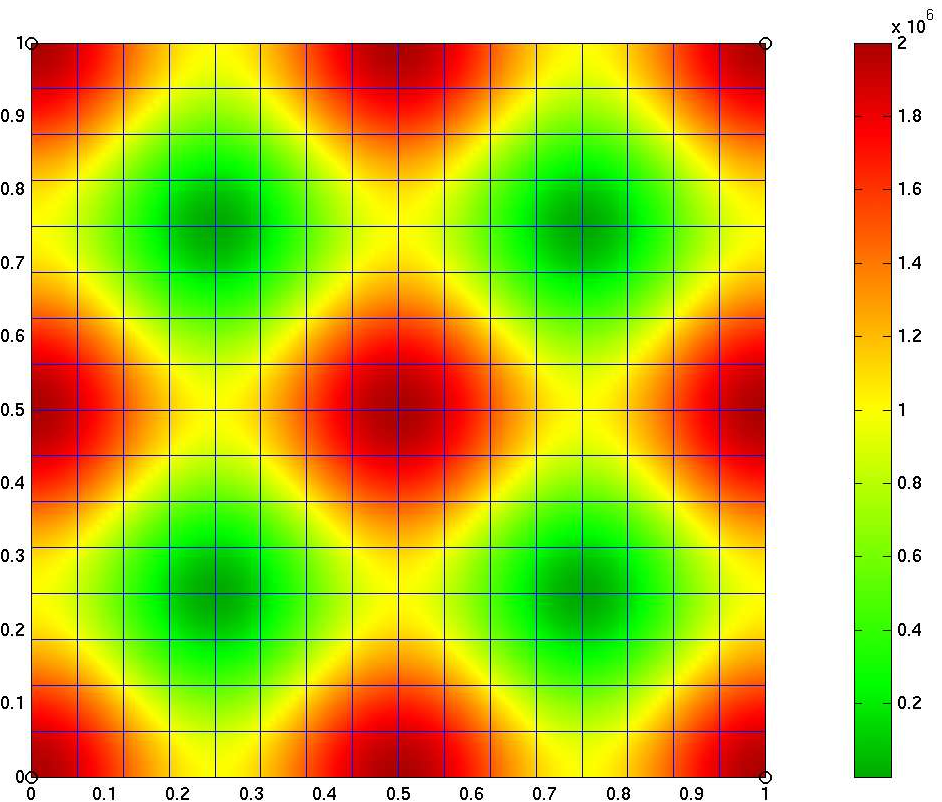
\includegraphics[width=0.48\textwidth]{figs/box}
	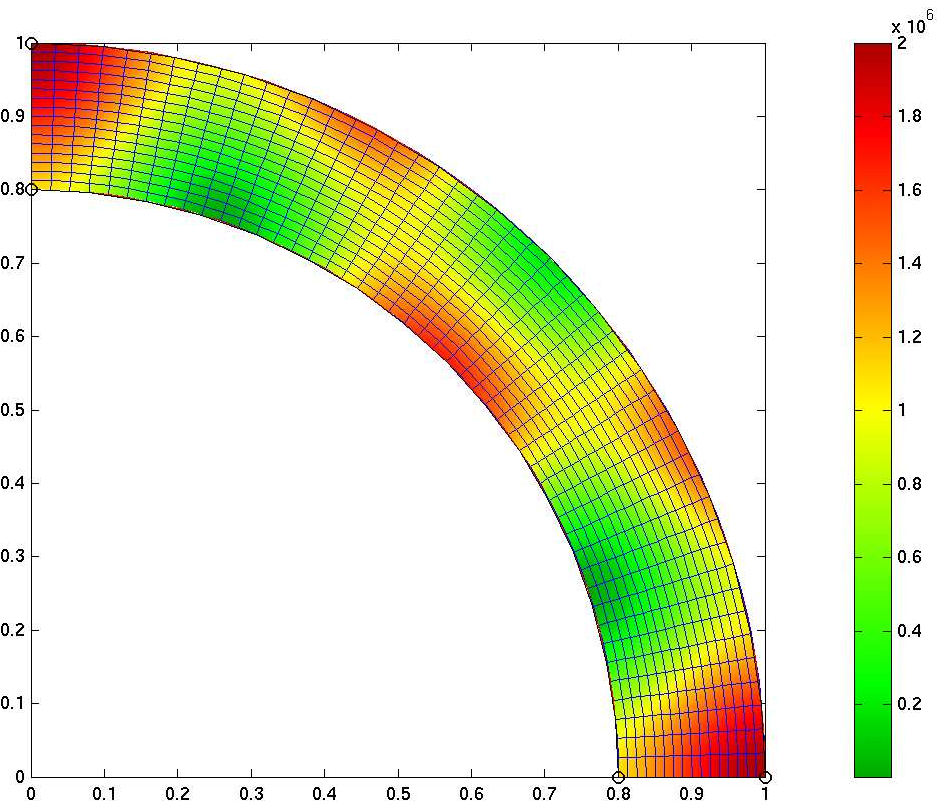
\includegraphics[width=0.48\textwidth]{figs/fan}
	\caption{\label{fig:mesh2d} The two dimensional meshes used in
          our tests. The color corresponds to the value of the
          coefficient $\mu(\bs x)$.}
\end{figure}
\begin{figure}
	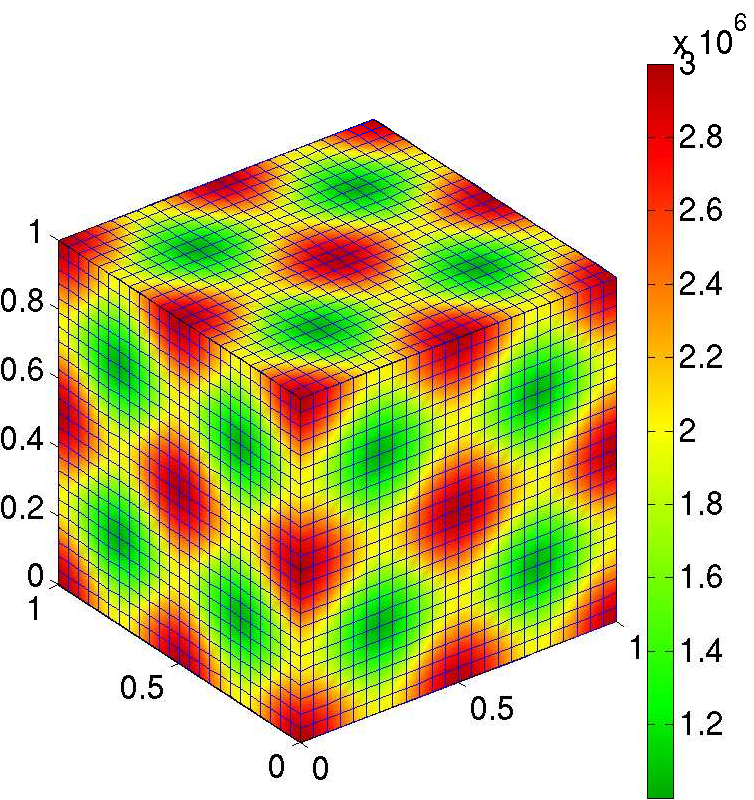
\includegraphics[width=0.48\textwidth]{figs/box3a}
	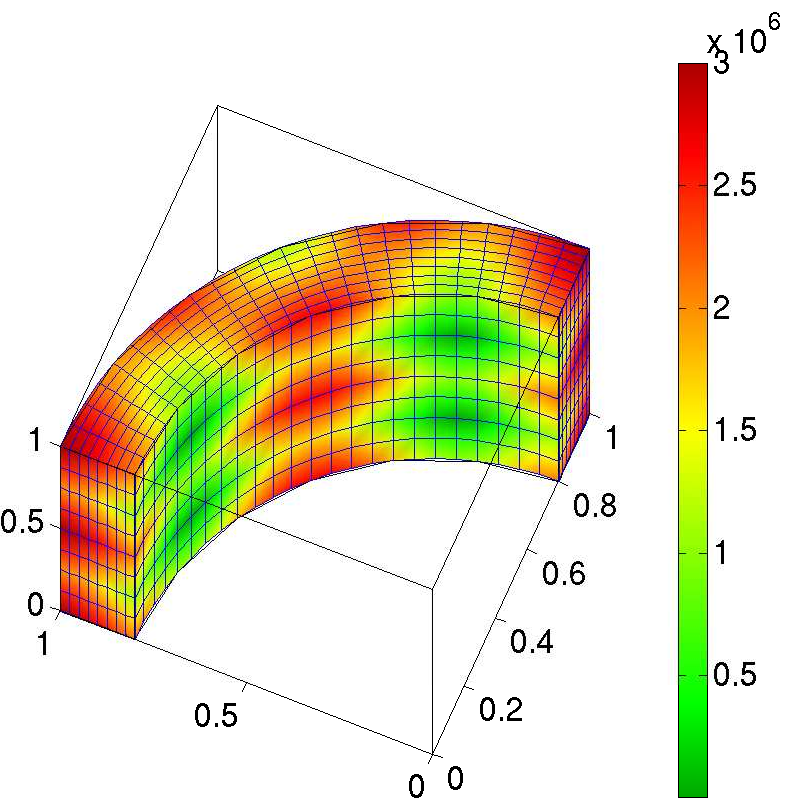
\includegraphics[width=0.48\textwidth]{figs/fan3a}
	\caption{\label{fig:mesh3d} The three dimensional meshes used
          in our tests. The color corresponds to the value of the
          coefficient $\mu(\bs x)$.}
\end{figure}




\subsection{Results for test problems}\label{subsec:results}
Here, we summarize our results for the test problems and present
comprehensive comparisons of the performance of our algorithms for the
solution of high-order discretizations of \eqref{eq:Poisson}.  The
Tables~\ref{tab:box}\ldots present the number of multigrid v-cycles or
of conjugate gradient (CG) iterations required to reduce the norm of
the discrete residual by a factor of $10^8$ for our test problems. In
particular, these tables show:
\begin{itemize}
\item[$\bullet$] The first column gives the polynomial \emph{order}
  used in the finite element discretization.
\item[$\bullet$] The columns entitled by \emph{MG as solver} report
  the number of v-cycles needed when multigrid is used as a
  solver. The subcolums are:
  \begin{itemize}
  \item \emph{Jacobi(3)} denotes that 3 pre-smoothing and 3
    post-smoothing steps of a pointwise Jacobi smoother are used on
    each level.
  \item \emph{Cheb(3)} denotes that Chebyshev-accelerated Jacobi
    smoothing is used. Again, we use 3 pre-smoothing and 3
    post-smoothing steps. The maximal eigenvalue required by the
    Chebyshev method is estimated using \todo{XX iterations of
      Lanczos}.
  \item \emph{SSOR(2)} denotes that a symmetric successive
    over-relaxation method is employed, where 2 pre-smoothing and 1
    post-smoothing step are employed. Note that each SSOR smoothing
    iteration amounts to a forward and a backward step, and thus
    requires double the computational work compared to Jacobi
    smoothing.\footnote{This ignores aspects occurring in parallel
      environments, where Gauss-Seidel smoothing---such as SSOR---can
      be challenging to implement and requires more communication in
      distributed memory environments.}  \todo{Is this really a
      2/1?}  The SSOR smoother is based on a lexicographic ordering of
    the unknowns. \gsnote{use different ordering too?}
  \end{itemize}
  Note that for each of the smoothers we results for high-order
  $h$-multigrid (columns marked by \emph{h}; see
  Section~\ref{subsec:h}) as well as for $p$-multigrid (columns marked
  by \emph{p}; see Section~\ref{subsec:p}). For $p$-multigrid, we
  restrict ourselves to orders that are powers of 2. After coarsening
  in $p$ as till $p=1$, and then coarsen in $h$.
\item[$\bullet$] The columns entitled with \emph{MG with pCG} presents
  our results obtained when multigrid is uses as preconditioner in a
  CG algorithm. The sub-columns are as described above.
\item[$\bullet$] The columns headed by \emph{linearized pCG} present
  the number of CG iterations needed to solve the high-order system
  preconditioned with the low-order operator based on the high-order
  node points (see Section~\ref{subsec:low}). In our implementation,
  the low-order system is solved using a direct factorization method.
  The sub-column headed by \emph{GLL} indicates that the non-evenly
  spaces GLL points are used in the low-order system, where
  \emph{unif.} indicates that a uniform node spacing is used for the
  low-order operator.
\end{itemize}


\begin{table}
  \caption{\label{tab:box} Results for two-dimensional unit square
    with constant coefficient $\mu\equiv 1$.  A total of 3 grids were
    used, the finest grid was $32\times 32$, and the coarsest was
    $8\times 8$ \todo{still true?}.}
  \centering
  \begin{tabular}{|r|c c|c c|c c||c c|c c|c c||c c|} 
    \hline
    & \multicolumn{6}{c||}{MG as solver} & \multicolumn{6}{c||}{MG with pCG} & \multicolumn{2}{r|}{linearized} \\
    \cline{2-13}
    \!\!\! order \!\!\!\! &  \multicolumn{2}{c|}{\!\scriptsize  Jacobi(3)\!} &  \multicolumn{2}{c|}{\!\scriptsize Cheb(3)\!} & \multicolumn{2}{c||}{\!\scriptsize  SSOR(2)\!} & \multicolumn{2}{c|}{\!\scriptsize Jacobi(3)\!} &  \multicolumn{2}{c|}{\!\scriptsize Cheb(3)\!} & \multicolumn{2}{c||}{\!\scriptsize SSOR(2)\!} & \multicolumn{2}{r|}{pCG}\\
\hline
 & $h$ & $p$ & $h$ & $p$& $h$ & $p$& $h$ & $p$& $h$ & $p$& $h$ & $p$& GLL & unif.\\
 \cline{2-15}
1 & 7 & & 5 & & 4 & & 6 & & 4 & & 4 & & 1 & 1  \\
2 & 10 & 13 & 5 & 6 & 4 & 5 & 7 & 7 & 4 & 5 & 4 & 4 & 16 & 16 \\
3 & 9 & & 6 & & 4 & & 7 & & 5 & & 4 & & 18 & 19  \\
4 & 10 & 19 & 6 & 7 & 4 & 5 & 8 & 8 & 5 & 6 & 4 & 4 & 20 & 23 \\
5 & 12 & & 8 & & 5 & & 9 & & 6 & & 4 & & 22 & 26  \\
6 & 12 & & 9 & & 5 & & 9 & & 6 & & 4 & & 25 & 31  \\
7 & 16 & & 12 & & 6 & & 10 & & 8 & & 5 & & 26 & 36  \\
8 & 17 & 29 & 13 & 11 & 7 & 6 & 10 & 11 & 8 & 8 & 5 & 5 & 28 & 42 \\
16 & 40 & 49 & 33 & 27 & 13 & 11 & 16 & 17 & 13 & 13 & 8 & 8 & 41 & 88\\
\hline
  \end{tabular}
\end{table}


\begin{table}
  \caption{\label{tab:2d-fan} Results for two-dimensional warped geometry
    with varying coefficient \todo{$\mu(\bs x) =$}.}
  \centering
  \begin{tabular}{|r|c c|c c|c c||c c|c c|c c||c c|} 
    \hline
    & \multicolumn{6}{c||}{MG as solver} & \multicolumn{6}{c||}{MG with pCG} & \multicolumn{2}{r|}{linearized} \\
    \cline{2-13}
    \!\!\! order \!\!\!\! &  \multicolumn{2}{c|}{\!\scriptsize  Jacobi(3)\!} &  \multicolumn{2}{c|}{\!\scriptsize Cheb(3)\!} & \multicolumn{2}{c||}{\!\scriptsize  SSOR(2)\!} & \multicolumn{2}{c|}{\!\scriptsize Jacobi(3)\!} &  \multicolumn{2}{c|}{\!\scriptsize Cheb(3)\!} & \multicolumn{2}{c||}{\!\scriptsize SSOR(2)\!} & \multicolumn{2}{r|}{pCG}\\
\hline
 & $h$ & $p$ & $h$ & $p$& $h$ & $p$& $h$ & $p$& $h$ & $p$& $h$ & $p$& GLL & unif.\\
 \cline{2-15}
1 & 18 & & 15 & & 6 & & 11 & & 10 & & 5 & & 1 & 1  \\
2 & 25 & 31 & 20 & 20 & 7 & 8 & 14 & 15 & 12 & 13 & 6 & 7 & 17 & 17 \\
3 & 27 & & 21 & & 8 & & 15 & & 13 & & 7 & & 19 & 20  \\
4 & 36 & 350 & 24 & 57 & 10 & 10 & 17 & 18 & 14 & 15 & 7 & 8 & 21 & 25 \\
5 & 39 & & 30 & & 12 & & 18 & & 15 & & 8 & & 23 & 28  \\
6 & 63 & & 34 & & 13 & & 20 & & 17 & & 9 & & 25 & 31  \\
7 & 58 & & 40 & & 15 & & 22 & & 18 & & 9 & & 26 & 37  \\
8 & 106 & 350 & 46 & 350 & 17 & 15 & 23 & 24 & 20 & 20 & 10 & 10 & 26 & 41 \\
16 & 350 & 350 & 350 & 350 & 35 & 31 & 35 & 37 & 31 & 30 & 14 & 15 & 33 & 72 \\
\hline
  \end{tabular}
\end{table}


\begin{table}
  \caption{\label{tab:3d-box} Results for three-dimensional cube geometry
    with constant coefficient $\mu(\bs x) \equiv 1$.}
  \centering
  \begin{tabular}{|r|c c|c c|c c||c c|c c|c c||c c|} 
    \hline
    & \multicolumn{6}{c||}{MG as solver} & \multicolumn{6}{c||}{MG with pCG} & \multicolumn{2}{r|}{linearized} \\
    \cline{2-13}
    \!\!\! order \!\!\!\! &  \multicolumn{2}{c|}{\!\scriptsize  Jacobi(3)\!} &  \multicolumn{2}{c|}{\!\scriptsize Cheb(3)\!} & \multicolumn{2}{c||}{\!\scriptsize  SSOR(2)\!} & \multicolumn{2}{c|}{\!\scriptsize Jacobi(3)\!} &  \multicolumn{2}{c|}{\!\scriptsize Cheb(3)\!} & \multicolumn{2}{c||}{\!\scriptsize SSOR(2)\!} & \multicolumn{2}{r|}{pCG}\\
\hline
 & $h$ & $p$ & $h$ & $p$& $h$ & $p$& $h$ & $p$& $h$ & $p$& $h$ & $p$& GLL & unif.\\
 \cline{2-15}
1 & 6 & & 5 & & 4 & & 5 & & 4 & & 3 & & 1 & 1  \\
2 & 7 & 7 & 5 & 5 & 4 & 4 & 6 & 6 & 4 & 5 & 3 & 4 & 26 & 26 \\
3 & 9 & & 6 & & 4 & & 7 & & 5 & & 4 & & 29 & 33  \\
4 & 11 & 10 & 8 & 7 & 5 & 4 & 7 & 7 & 6 & 6 & 4 & 4 & 33 & 42 \\
5 & 14 & & 10 & & 5 & & 8 & & 7 & & 5 & & 36 & 50  \\
6 & 16 & & 12 & & 6 & & 9 & & 8 & & 5 & & 40 & 61  \\
7 & 20 & & 15 & & 7 & & 10 & & 9 & & 5 & & 44 & 74  \\
8 & 22 & 18 & 17 & 15 & 7 & 6 & 11 & 10 & 10 & 8 & 5 & 5 & 52 & 99 \\
\hline
  \end{tabular}
\end{table}

\begin{table}
  \caption{\label{tab:3d-fan} Results for three-dimensional warped geometry
    with coefficient \todo{$\mu(\bs x)=$}.}
  \centering
  \begin{tabular}{|r|c c|c c|c c||c c|c c|c c||c c|} 
    \hline
    & \multicolumn{6}{c||}{MG as solver} & \multicolumn{6}{c||}{MG with pCG} & \multicolumn{2}{r|}{linearized} \\
    \cline{2-13}
    \!\!\! order \!\!\!\! &  \multicolumn{2}{c|}{\!\scriptsize  Jacobi(3)\!} &  \multicolumn{2}{c|}{\!\scriptsize Cheb(3)\!} & \multicolumn{2}{c||}{\!\scriptsize  SSOR(2)\!} & \multicolumn{2}{c|}{\!\scriptsize Jacobi(3)\!} &  \multicolumn{2}{c|}{\!\scriptsize Cheb(3)\!} & \multicolumn{2}{c||}{\!\scriptsize SSOR(2)\!} & \multicolumn{2}{r|}{pCG}\\
\hline
 & $h$ & $p$ & $h$ & $p$& $h$ & $p$& $h$ & $p$& $h$ & $p$& $h$ & $p$& GLL & unif.\\
 \cline{2-15}
1 & 350 & & 10 & & 4 & & 11 & & 7 & & 4 & & 1 & 1  \\
2 & 20 & 21 & 18 & 18 & 7 & 7 & 10 & 10 & 9 & 10 & 5 & 5 & 27 & 27 \\
3 & 25 & & 21 & & 8 & & 11 & & 10 & & 6 & & 30 & 33  \\
4 & 29 & 27 & 24 & 23 & 9 & 9 & 12 & 12 & 11 & 11 & 6 & 6 & 32 & 42 \\
5 & 36 & & 30 & & 11 & & 14 & & 13 & & 7 & & 35 & 50  \\
6 & 41 & & 34 & & 13 & & 15 & & 14 & & 8 & & 38 & 60  \\
7 & 48 & & 40 & & 14 & & 17 & & 15 & & 8 & & 40 & 70  \\
8 & 50 & 45 & 42 & 38 & 15 & 14 & 17 & 16 & 16 & 14 & 9 & 8 & 40 & 81 \\
\hline
  \end{tabular}
\end{table}


%%% anisotropy - stretched fan
%\begin{table}
%  \caption{\label{tab:fan-aniso} Number of CG iterations/v-cycles to converge to a relative tolerance of $10^{-8}$ for $h$-Multigrid applied to high-order operators on a stretched fan domain. A total of 3 grids were used, the finest grid was $48\times 16$, and the coarsest was $12\times 4$. For orders $2,4$, and $8$, we also evaluated the option of first coarsening in $p$ as $p_{coarse} = p_{fine}/2$, till $p=1$, and then coarsen in $h$. The coarsest grid in this case is a $12\times 4$ grid with $p=1$. The number of CG iterations/v-cycles for this case is given in the $p$ column.}
%		\centering
%    \begin{tabular}{|l|c|c|c|c|c|c|c|c|c|c|c|c|r|} 
%\hline
%		        & \multicolumn{6}{c|}{Multigrid} & \multicolumn{6}{c|}{MG pCG} &          linearized \\
%												 \cline{2-13}
%					order &  \multicolumn{2}{c|}{\scriptsize  Jacobi(3)} &  \multicolumn{2}{c|}{\scriptsize Chebyshev(3)} & \multicolumn{2}{c|}{\scriptsize  SSOR(2)} & \multicolumn{2}{c|}{\scriptsize Jacobi(3)} &  \multicolumn{2}{c|}{\scriptsize Chebyshev(3)} & \multicolumn{2}{c|}{\scriptsize SSOR(2)} & pCG\\
%		\hline
%		 & $h$ & $p$ & $h$ & $p$& $h$ & $p$& $h$ & $p$& $h$ & $p$& $h$ & $p$& \\
%		 \cline{2-13}
% 1 &       16 &      &        21 &        &       6 &         &       9 &         &       10 &       &       5 &      & 5  \\
% 2 &       22 &  23  &        24 &  24    &       7 &   7     &      10 &  11     &       11 &  11   &       5 &   5  & 67  \\
% 3 &        - &      &        54 &        &       8 &         &      55 &         &       17 &       &       6 &      & 160  \\
% 4 &        - &  -   &        97 &  92    &      14 &   13    &       - &         &       23 &  22   &       9 &   8  & 262  \\
% 5 &        - &      &       313 &        &      22 &         &       - &         &       41 &       &      11 &      & 444  \\
% 6 &        - &      &         - &        &      76 &         &       - &         &       73 &       &      21 &      & 654  \\
% 7 &        - &      &         - &        &     259 &         &       - &         &      161 &       &      38 &      & 941  \\
% 8 &        - &  -   &         - &  -     &       - &    -    &       - &         &        - & 271   &      88 &  72  & 1150  \\
%\hline
%	  \end{tabular}
%\end{table}
%



%% 3D





\section{Discussion and conclusions}

%Finalize and discuss ramifications.

\todo{Preliminary list of conclusions:}
\begin{itemize}
\item Chebyshev improves significantly over Jacobi smoothing and is
  competitive with SSOR
\item Point smoothers performed reasonably well for all tested orders,
  in particular in combination with pCG
\item low-order preconditioner competitive w.r. to number of
  iterations; thus a good option as preconditioner when using AMG for
  unstructured high-order meshes

%\item Using Jacobi-based multigrid as preconditioner in the conjugate
%  gradient method, the number of iterations for polynomial orders
%  $p=2,3$ is similar to the number of iterations for linear elements.
%  In general, for the same number of unknowns one can expect better
%  accuracy for higher polynomial order. This advantage has to be
%  contrasted with the fact that high-order operators are less sparse
%  and thus their application to vectors is more time consuming.  Using
%  Jacobi-based smoothers is attractive from a parallel perspective
%  since no coloring of unknowns as in SSOR is necessary.
%\item Both, high-order $h$-multigrid as well as $p$-multigrid yield
%  significantly faster convergence in terms of the number of
%  iterations than preconditioning with the low-order
%  operator. Although low order operators are sparser and thus faster
%  to apply, the significant larger number of iterations results in
%  larger time-to-solution, in particular since the high-order operator
%  must be used to compute the residual on the finest mesh.
%\item For problems that only require a small number of smoothing
%  steps, using Chebyshev acceleration for the Jacobi smoother does not
%  improve the convergence. In all our tests, SSOR smoothing results in
%  the fastest convergence, in particular for orders $p\ge
%  4$. \gsnote{Revisit.}
\end{itemize}


\bibliographystyle{siam}
\bibliography{ccgo}


\end{document}
